\documentclass[a4paper,titlepage]{book}     	%base
\usepackage[T1]{fontenc}
\usepackage[utf8]{inputenc}
\usepackage[english]{babel}
\usepackage{geometry} 							%margini
\geometry{a4paper, top=2.5cm, bottom=2.3cm, left=2.3cm, right=2.3cm, heightrounded, bindingoffset=1cm}
\usepackage{verbatim}  							%ambiente commento

\usepackage[nouppercase]{frontespizio}%frontespizio
\usepackage{pdflscape}    						%pagina orizzontale
\usepackage{emptypage}

\usepackage{amsmath, amssymb, mathtools,bm} 					%matematica
\usepackage{siunitx}\sisetup{exponent-product = \cdot}   

\usepackage[english]{varioref}							%vref
\usepackage{hyperref} 							%coll. ipertestuali   ->commentato per usarlo con pdfa
\hypersetup{hidelinks}
%,colorlinks=true,linkcolor=black,citecolor=blue, urlcolor=blue} 							%nascondi riquadri hyp.
\usepackage{booktabs} 							%tabelle
\usepackage{threeparttable}	
\usepackage{multirow}
\usepackage[labelfont=bf, font=small]{caption} 	%didascalie
\usepackage{import} 							%inkscape
\usepackage[toc,page]{appendix}




%bibliografia
\usepackage[autostyle]{csquotes} 				
\usepackage[backend=biber, style=numeric-comp, maxnames=1,sorting=none]{biblatex}  %  style=authoryear-comp, style=numeric-comp, sorting=none sorting=nyt,sortlocale=en_GB  maxnames=1,uniquelist=false,
\addbibresource{biblio.bib}

\AtEveryBibitem{%
	\ifentrytype{article}{
		\clearfield{eprint}%
		\clearfield{url}%
	}{}
	\ifentrytype{ARTICLE}{
		\clearfield{eprint}%
		\clearfield{url}%
	}{}
	\clearfield{issn}%
	\clearfield{doi}%
}


\newcommand{\aap}{Astronomy and Astrophysics}
\newcommand{\aapr}{Astronomy and Astrophysics Review}
\newcommand{\aaps}{Astronomy and Astrophysics, Supplement}
\newcommand{\apj}{Astrophysical Journal}
\newcommand{\apjl}{Astrophysical Journal, Letters}
\newcommand{\apjs}{Astrophysical Journal, Supplement}
\newcommand{\araa}{Annual Review of Astronomy and Astrophysics}
\newcommand{\baas}{Bulletin of the AAS}
\newcommand{\bain}{Bulletin Astronomical Institute of the Netherlands}
\newcommand{\mnras}{Monthly Notices of the Royal Astronomical Society}
\newcommand{\nat}{Nature}
\newcommand{\pasa}{Publications of the Astronomical Society of Australia}
\newcommand{\prl}{Physical Review Letters}


%numeri di pagina ai bordi e nomi capitoli fighi
\usepackage{fancyvrb}
\usepackage{fancyhdr}

\pagestyle{fancy}
\renewcommand{\chaptermark}[1]{\markboth{#1}{}}
\renewcommand{\sectionmark}[1]{\markright{\thesection\ #1}}
\fancyhf{}
\fancyhead[LE, RO]{\scshape\thepage}
\fancyhead[LO]{\scshape\small\nouppercase{\rightmark}}
\fancyhead[RE]{\scshape\small\nouppercase{\leftmark}}

%nuovi comandi
\newcommand{\sun}{\ensuremath{_\odot}} 	
\newcommand{\mzams}{M_\textup{ZAMS}}
\newcommand{\zzams}{Z_\textup{ZAMS}} 
\newcommand{\mdot}{\ensuremath{\dot{M}}}
\newcommand{\msun}{\ensuremath{M\sun}}
\newcommand{\rsun}{R_{\odot}}
\newcommand{\lsun}{L_{\odot}}
\newcommand{\zsun}{\ensuremath{Z\sun}}
\newcommand{\yr}{\text{yr}}
\newcommand{\rl}{\ensuremath{R_\textup{L}}}
\newcommand{\rlone}{\ensuremath{R_\textup{L,1}}}
\newcommand{\rltwo}{\ensuremath{R_\textup{L,2}}}
\newcommand{\mwr}{\ensuremath{M_\textup{WR}}}
\newcommand{\mbh}{\ensuremath{M_\textup{BH}}}

\newcommand{\micmap}[1]{\textcolor{red}{MM:\bf#1}}
\newcommand{\erika}[1]{\textcolor{green}{\bf#1}}
\usepackage{soul}
\usepackage{xcolor}

%sommario
\newenvironment{abstract}{\newpage \thispagestyle{empty} \vspace*{3\baselineskip}
	\begin{center}\Large\textbf\abstractname\end{center}
	\begin{quotation}
	}{\end{quotation}\clearpage}

%pdf-a
%\usepackage[a-1b]{pdfx}
%\usepackage[pdfa]{hyperref}
%\hypersetup{hidelinks} 

%%%%%%%%%%%%%%%%%%%%%%%%%%%%%%%%%%%%%%%%%%%%%%%%%%%%%%%%%%%%%%%%%%%
%%%%%%%%%%%%%%%%%%%%%%%%%%%%%%%%%%%%%%%%%%%%%%%%%%%%%%%%%%%%%%%%%%%
\begin{document}
\frontmatter

\begin{frontespizio}
	\Preambolo{\renewcommand{\frontinstitutionfont}{\fontsize{15}{12}\bfseries}}
	\Preambolo{\renewcommand{\frontdivisionfont}{\fontsize{16}{30}\selectfont}}
	\Preambolo{\renewcommand{\frontpretitlefont}{\fontsize{16}{20}\scshape}}
	\Preambolo{\renewcommand{\fronttitlefont}{\fontsize{19}{35}\bfseries}}
	\Preambolo{\renewcommand{\frontnamesfont}{\fontsize{15}{20}\bfseries}}
	\Preambolo{\renewcommand{\frontfixednamesfont}{\fontsize{13}{20}\selectfont}}

	\Istituzione{Università degli studi di Padova}
	\Logo[3cm]{logo}
	\Divisione{\vspace*{1mm}Dipartimento di Fisica e Astronomia ``Galileo Galilei'' }
	\Scuola{Master Degree in Astrophysics and Cosmology}
	\Titoletto{Final dissertation}
	%\Annoaccademico{2019--2020}
	\Piede{Academic Year 2021--2022}
	\Titolo{\vspace*{-15mm} Black hole - Wolf-Rayet binaries as \\ progenitors of binary black holes}
	\NCandidato {Candidate}
	\Candidato {Erika Korb}
	\NRelatore {Supervisor}{}
	\Relatore {Prof. Michela Mapelli}
	\NCorrelatore {Co-supervisor}{}
	\Correlatore {Dr.~Giuliano Iorio}
	\Rientro{2cm}
\end{frontespizio}	

\

\begin{abstract}
\addcontentsline{toc}{chapter}{Abstract}
In this thesis, I studied Wolf Rayet -- black hole (WR--BH) binary systems by means of the population-synthesis code \texttt{SEVN}. In particular, I investigated whether WR--BH binaries are the progenitors of the binary black holes observed with the gravitational wave detectors LIGO and Virgo. I focused my work on solar-metallicity systems and examined the formation of Cyg X-3, the only WR--BH candidate known so far in the Milky Way. I explored a 24-dimension parameter space with two possible values for the solar metallicity, three core-collapse supernova models and four natal kick options. For each of the 24 combinations, I generated a physically motivated population of $10^6$ binaries with \texttt{SEVN} and determined the influence of this parameter space on the evolution of WR--BH systems.\\

I found that $\gtrsim 90\%$ of the simulated merging binary black holes evolved through the WR--BH configuration. Cyg X-3 is likely a progenitor of these systems, with a probability $\gtrsim 75\%$ in the most conservative cases. These results are robust and are not significantly affected by the parameter space explored. Eventually, I analyzed in detail the evolution of binaries similar to Cyg X-3 and found that the WR--BH phase is the result of two or three mass transfer episodes. The number and type of mass transfer processes are mainly affected by the core-collapse supernova model, even though a final common envelope is mandatory to form the Wolf-Rayet star in all the Cyg X-3 candidates that I considered.

My results highlight that WR--BH systems are almost a necessary evolutionary stage to produce merging binary black holes at solar metallicity. Therefore, additional and more accurate observations of binaries like Cyg X-3 emerge as one of the most promising possible characterizations of binary black hole progenitors, providing unique insights to their formation channels and to the mass transfer physics.\\

In the first chapter of this thesis, I introduced the possible tension between the spin and mass distribution of X-ray binaries and binary black holes. In the second chapter I discussed the uncertainties and possible fates of the sample of observed WR--BH binaries, including the characterization of Cyg X-3. Also, the second chapter contains a discussion on the current single stellar evolution theory and mass transfer models, highlighting their limits and role in binary evolution. In the third chapter I described the code \texttt{SEVN} and the choice of the initial conditions. I presented my results in the fourth chapter and drew my conclusions in the fifth chapter. 
\end{abstract}

\tableofcontents
\addcontentsline{toc}{chapter}{Contents}

%%%%%%%%%%%%%%%%%%%%%%%%%%%%%%%%%%%%%%%%%%%%%%%%%%%%%%%%%%%%%%%%%
\mainmatter

% Binary black hole quando si intende una binaria con 2 black hole, black hole binary quando uno dei due può non essere un black hole
% In questa tesi intendo sempre due buchi neri
\chapter{Demography of binary black holes}\label{ch:GW}

\paragraph{The new gravitational wave era} In September 2015, the detection of the first gravitational wave event, GW150914, not only confirmed the existence of binary systems made of two stellar black holes but also demonstrated that such systems are capable of merging via emission of gravitational waves within a Hubble time $H_0^{-1}$ \cite{Abbott2016firstGW}. In March 2020, the LIGO, Virgo and KAGRA Collaboration (hereafter, \emph{LVC}) ended the third observing run and, by November 2021, produced the third gravitational-wave transient catalog (GWTC-3), revealing a total of $\sim 80$ merging binary black holes discovered with the gravitational wave detectors. Overall, GWTC-3 revealed $\sim 90$ mergers of compact objects binaries, including also double neutron star and neutron star-black hole systems that will not be considered in this thesis \cite{GWTC-3}. 


\paragraph{Two main evolutionary channels}
The formation pathways of binary black holes are an active field of research and can be divided into two main evolutionary scenarios: isolated binary or dynamically active environments. They can be investigated analyzing of the features in the distribution of the masses, spins and related quantities: different formation channels lead to different predictions on black hole mass, mass ratio $q=M_2/M_1$ ($M_1 \geq M_2$), spin alignment and magnitude.
 
In the isolated binary evolution scenario, tidal interactions and mass transfer episodes are thought to be so efficient to favour the production of compact objects with similar masses ($q \sim 1$) \cite{giacobbomapelli2018_mobse_fryer} with spins aligned and parallel to the orbital angular momentum \cite{Kalogera2000_spinaligned}. Binaries that evolve in a dynamically active environment likely undergo exchanges and hierarchical mergers, allowing for more asymmetric masses ($q << 1$) \cite{Rastello2021_dynamics} and favoring an isotropic spin orientation \cite{Rodriguez2016_BHspins}.

Single stellar evolution prohibits the formation of black hoes in the pair-instability mass gap $\sim 60 - 120 ~\msun$ \cite{spera2017_pisnSNe}: the existence of black holes in the gap, like the ones of GW190521 ($\sim 66~\msun$ and $\sim 85~\msun$ \cite{GW190521_abbott2020}), requires either a hierarchical merger history or a different modeling in the stellar evolution (for instance, lowering the rate of the triple-$\alpha$ reaction can push to higher masses the lower boundary of the mass gap \cite{MassGapStellarEvo_Costa2021}).

The spin magnitude of the primary (first formed) and secondary (last formed) black hole can be related to the dominant mass transfer processes. On the one hand, X-ray binaries observations indicate that the secondary black hole can be spun-up by tides \cite{spinupBH_Bavera2020}. On the other hand, primary black holes formed through a common envelope are thought to be almost zero-spinning black holes because their progenitors dissipated the angular momentum when they lost their envelope \cite{spinBH_Qin2018}.  Nevertheless, the observation of high-mass X-ray binaries with fast spinning black holes and main sequence companions suggests that the current modeling and understanding of the angular momentum transport in single and stellar binary evolution is still rather poor and needs further investigation \cite{spinfastBH_Qin2019}. Moreover, spins are difficult to constrain with a good precision in gravitational-wave signals (they cause second-order effects in the gravitational waveform) and their connection to the progenitor evolution is further challenged by the core-collapse supernova, which modifies both the magnitude and the orientation of the spin of the new-born black hole \cite{GWTC-3_interpretation}.

\paragraph{Chapter outline}
In the following sections I will explain the theoretical background and observational methodology used to determine the properties of binary black holes  revealed with the gravitational waves (hereafter, \emph{LVC binary black holes}) and of their progenitor candidates, the X-ray binaries. Then, I will discuss the possible tension between the binary black holes and X-ray binaries mass and spin distributions. 


\section{Gravitational waves}\label{sec:GW}
\subsection{Theory and methods for parameter estimation}\label{subsec:GWtheorymethod}
\paragraph{A match-filtering method} The detection and characterization of the binaries observed with gravitational waves relies on matched-filtering techniques and Bayesian analysis. 

First, the signal is detected with the match-filtering technique. The detection pipeline filters the recorded signal with waveform templates generated by numerical relativity calculations. Different binary properties produce different waveforms, therefore a match in the signal not only reveals a detection but allows an approximate estimate of the binary parameters.

Once the signal is detected, general-relativity models that include, for instance, spin precession are used to refine the waveform template and the fit. Eventually, Bayesian analysis is carried out on each data-set to derive posterior distributions of source parameters: the final best estimates are usually the median values of the posterior distribution with uncertainty given by the 90\% credible interval.

\paragraph{Spin determination} A black hole binary undergoing a quasi-circular inspiral is characterized by fifteen parameters\footnote{The $16^{th}$ parameter, eccentricity, is currently neglected in the LVC analysis for computational reasons.}: eight intrinsic (mass $M_i$ and three-dimensional components of the spin vectors $\vec{S}_i$ for each $i$-th black hole) and seven extrinsic, for the sky location and orbit orientation (right ascension $\alpha$, declination $\delta$, luminosity distance $d_L$, orbital inclination $\iota$, polarization angle $\Phi$, time of coalescence $t_c$ and phase at the coalescence $\phi_c$) \cite{GWTC-1}.

In reality, the three spin vectors are the most difficult parameters to characterize because they imprint a second-order effect in the waveform, requiring advanced numerical relativity calculations to be correctly modeled. In place of the six spin vectors, the pipeline analysis fits six effective spin parameters that are slightly easier to obtain from the observations: the two dimensionless spin magnitudes $\chi_i$, the two polar tilt angles $\theta_i$, the effective spin $\chi_{eff}$ and the effective precessing spin $\chi_p$. All the values are calculated at the reference frequency of 20 Hz.

The \emph{dimensionless spin} $\chi_i$ quantifies the amplitude of the spin by measuring how much the black hole is close to being a Schwarzschild, non-rotating black hole ($\chi_i = 0$) or to a maximally-spinning Kerr black hole ($\chi_i = 1$)

\begin{equation}\label{eq:chispin}
	\chi_i = \frac{|\vec{S}_i| c}{G M_i} \quad  \in [0,1]   \qquad \qquad i=1,2,
\end{equation}

where $\vec{S}_i$ is the spin vector, $G$ the gravity constant, and $c$ the speed of light.

The two polar angles $\theta_i$ measure the inclination of each black hole spin with respect to the orbital angular momentum $\hat{L}_N$ and enter in the definition of both the effective spin $\chi_{eff}$ and the effective precessing spin $\chi_p$. The \emph{effective spin} $\chi_{eff}$ measures the mass-weighted components of black hole spins that are aligned with the Newtonian orbital angular momentum $\hat{L}_N$ (normal to the orbital plane)

\begin{equation}\label{eq:chieff}
	\chi_{eff} = \frac{M_1 \chi_1 \cos\theta_1 + M_2 \chi_2 \cos\theta_2}{M_1 + M_2}
\end{equation}

The \emph{effective precessing spin}, which measures the dominant spin projected on the orbital plane, that eventually causes the relativistic precession of the orbital plane itself

\begin{equation}\label{eq:chip}
	\chi_p = \max \left\{\chi_1 \sin\theta_1,~ \left(\frac{3+4q}{4+3q}\right) q\chi_2 \sin\theta_2\right\}
\end{equation}

where $q=M_2/M_1$ is the binary mass ratio \cite{GWTC-3_interpretation}.



\paragraph{A toy model for the main parameter estimation} Beside Bayesian analysis, it is still possible to obtain order-of-magnitude estimates of the key quantities that shape the waveform, like the masses, by simply using as toy model a circular binary that converts all the orbital energy lost into gravitational wave radiation. \\

According to the theory of the general relativity, the amplitude of  gravitational waves is proportional to the second derivative with respect to time of the mass quadrupole moment of the compact source.  Explicit calculation of the quadrupole moment of a circular binary relates the amplitude $h$  of the gravitational wave emitted to the luminosity distance $d_L$, the gravitational wave frequency $\nu_{\rm GW}$ and the chirp mass $\mathcal{M}$ according to \cite{MaggioreGW,GWreview}:

\begin{equation}\label{eq:h}
h = \frac{4}{d_L} \left(\frac{G \mathcal{M}}{c^2}\right)^{5/3} \left(\frac{\pi \,{}\nu_{\rm GW}}{c}\right)^{2/3} 
\end{equation}

The \emph{chirp mass} $\mathcal{M}$ is defined as a combination of the masses of the binary and is defined in every time interval of the signal by the different value $\nu_{\rm GW}$ and derivative $\dot{\nu}_{\rm GW}$ of the gravitational wave frequency, as follows

\begin{equation}\label{eq:Mchirp}
\mathcal{M} = 
\frac{(M_1\,{}M_2)^{3/5}}{(M_1+M_2)^{1/5}} =
\frac{c^3}{G} \left(\frac{5}{96}~ \pi^{-8/3}~\nu_{\rm GW}^{-11/3}~ \dot{\nu}_{\rm GW}\right)^{3/5}
\end{equation}

The chirp mass is easily obtainable from the signal analysis by Fourier-transforming the recorded amplitude time-series into a frequency time-series, as shown in Fig.\ \ref{fig:GW150914}. By re-arranging the definition of the chirp mass, it is possible to show that knowing the chirp mass puts a lower limit to the total mass of the system

\begin{equation}
(M_1 + M_2)_{\rm min} = 4^{3/5} \mathcal{M} \sim 2.3~\mathcal{M}
\end{equation}


The gravitational wave frequency dependence in Eq.\ \ref{eq:h} already encloses all the information on the compactness of the orbit. The binary considered in the toy model is circular so its mass quadrupole moment is symmetric under a $180^\circ$ rotation: every half-orbit the gravitational wave produced has the same phase. In other words, a circular binary produces a gravitational wave  with frequency that is twice the orbital frequency:  $\nu_{\rm GW} = 2 \nu_{\rm s}$. \\

As the binary spirals-in, the orbit tightens and the orbital frequency increases, causing a rise also in the gravitational wave frequency and in the amplitude of the signal, according to Eq.\ \ref{eq:h}: it is the so-called \emph{chirp signal}. The peak of the signal, both in terms of frequency and amplitude, is reached at coalescence, when the orbital separation reaches its minimum and is just the sum of the two Schwarzschild radii %in alternativa potrei prendere R_ISCO che non rompe Kepler

\begin{equation}\label{eq:Rcoalescence}
R_{\rm coalescence} = \frac{2G}{c^2} (M_1 + M_2)
\end{equation}

Using Kepler's third law and the relation $\nu_{\rm GW} = 2 \nu_{\rm s}$, the peak frequency of the gravitational wave $\nu_{\rm GW, peak}$ can be related to the total mass of the binary by


\begin{equation}\label{eq:nupeak}
	\nu_{\rm GW, max} = \frac{1}{\pi \sqrt{8}}\frac{c^3}{G\,{}(M_1+M_2)}
\end{equation}




\paragraph{Coalescence to determine masses, orbital separation and luminosity distance} Eq.\ \ref{eq:nupeak} and \ref{eq:Mchirp} show that precise measurements on the inspiral and peak frequency provide the chirp and total mass of the system. Measuring the peak frequency, therefore the total mass, also allows the determination of the orbital distance at coalescence. Given that the amplitude of the gravitational wave is the signal recorded by the detectors, it is possible to use Eq.\ \ref{eq:h} with the values known at the coalescence to obtain the luminosity distance of the source.


On the one hand, assuming a cosmological model, it is possible to convert the luminosity distance into the redshift of the source. On the other hand, gravitational wave observations provide an independent luminosity distance measurement that, coupled with electromagnetic counterpart observations, allows an independent method to estimate the Hubble cosmological parameter $H_0$ \cite{H0fromGW}.

Gravitational waves are stretched by the expansion of the Universe, therefore it is mandatory to use the redshift information to correct the parameters determined so far in the detector's frame and obtain the intrinsic ones in the source's frame. Because of the cosmological redshift $z$, the observed frequency of the gravitational wave is lower than the one emitted. The frequency-dependence enters in the determination of the chirp mass in Eq.\ \ref{eq:Mchirp} and, according to Eq.\ \ref{eq:nupeak}, a lower peak frequency results in an over-estimation of the source total mass. Eventually, both masses need to be reduced as

\begin{equation}\label{eq:Massesredshift}
	M_i^{source} = \frac{M_i^{det}}{(1+z)} \qquad \qquad i=1,2
\end{equation}


\begin{figure}[h]
	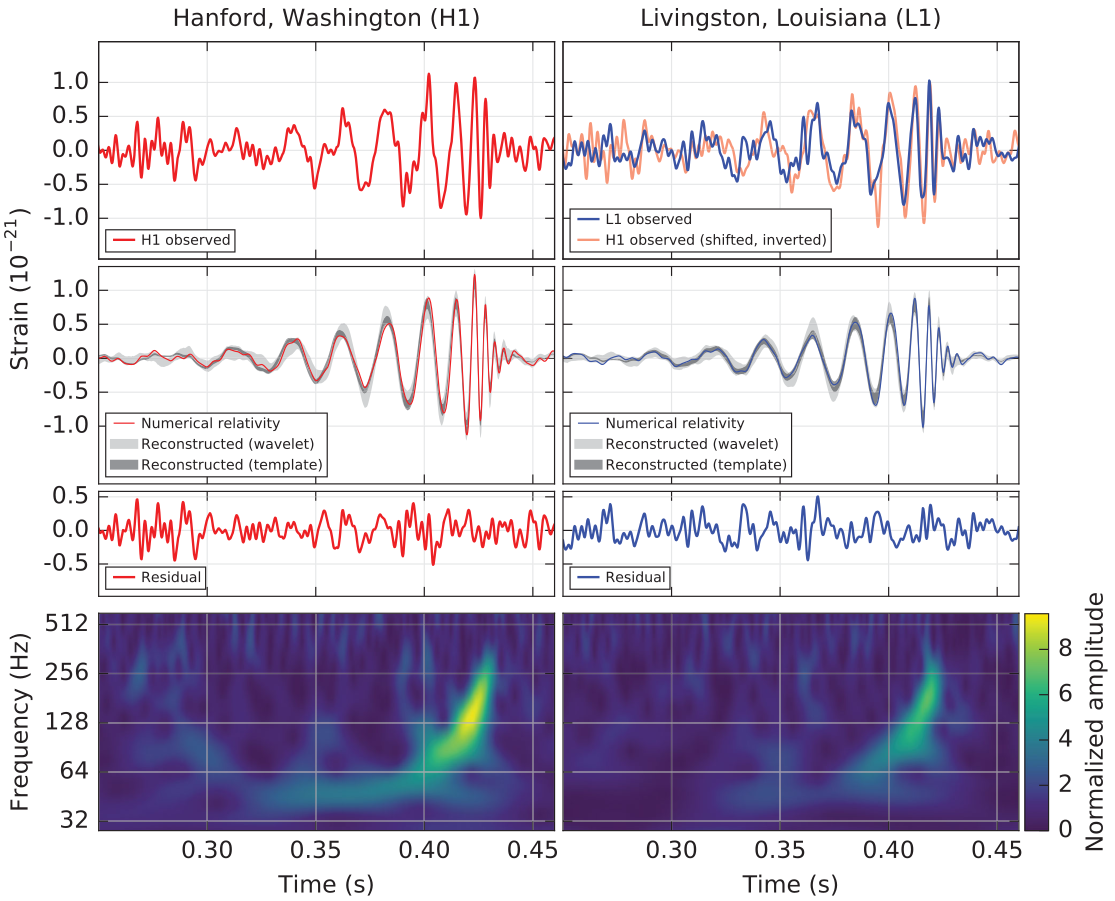
\includegraphics[width=\textwidth]{./images/GW150914.png}
	\caption{Signal detection of GW150914 \cite{Abbott2016firstGW}. \textit{Top:} amplitude time-series. \textit{Bottom:} frequency time-series.}\label{fig:GW150914}
\end{figure}

\paragraph{GW150914-like binaries} It is possible to apply the above formulas to get an order-of-magnitude estimate of any binary detection. For instance, the Bayesian analysis of the signal of GW150914 reported in Fig.\ \ref{fig:GW150914} revealed two black holes of masses $M_1=35.6^{+4.7}_{-3.1} ~ \msun$ and $M_2=30.6^{+3.0}_{-4.4} ~ \msun$ at redshift $z=0.09^{+0.03}_{0.03}$ within 90\% confidence intervals \cite{GWTC-1}. Using Eq.\ \ref{eq:Massesredshift}, the masses revealed in the detector frame where about 10\% heavier, respectively $M_1 \sim 39 ~ \msun$ and $M_1 \sim 33 ~ \msun$. The corresponding chirp mass was $\mathcal{M} \sim 30 \msun$ and the total mass $M \sim 70 ~ \msun$, meaning that at the coalescence the binary had a radius of only $R_{\rm coalescence} \sim 200~\text{km}$ and produced a peak gravitational wave at $\nu_{\rm GW, peak} \sim 300 ~\text{Hz}$. The binary had a luminosity distance of $d_L=410~\text{Mpc}$ and the gravitational wave was detected with an amplitude of $h \sim 10^{-21}~ \text{Hz}^{-1/2}$.


\begin{figure}[h]
	\begin{minipage}{.47\textwidth}
		\centering
		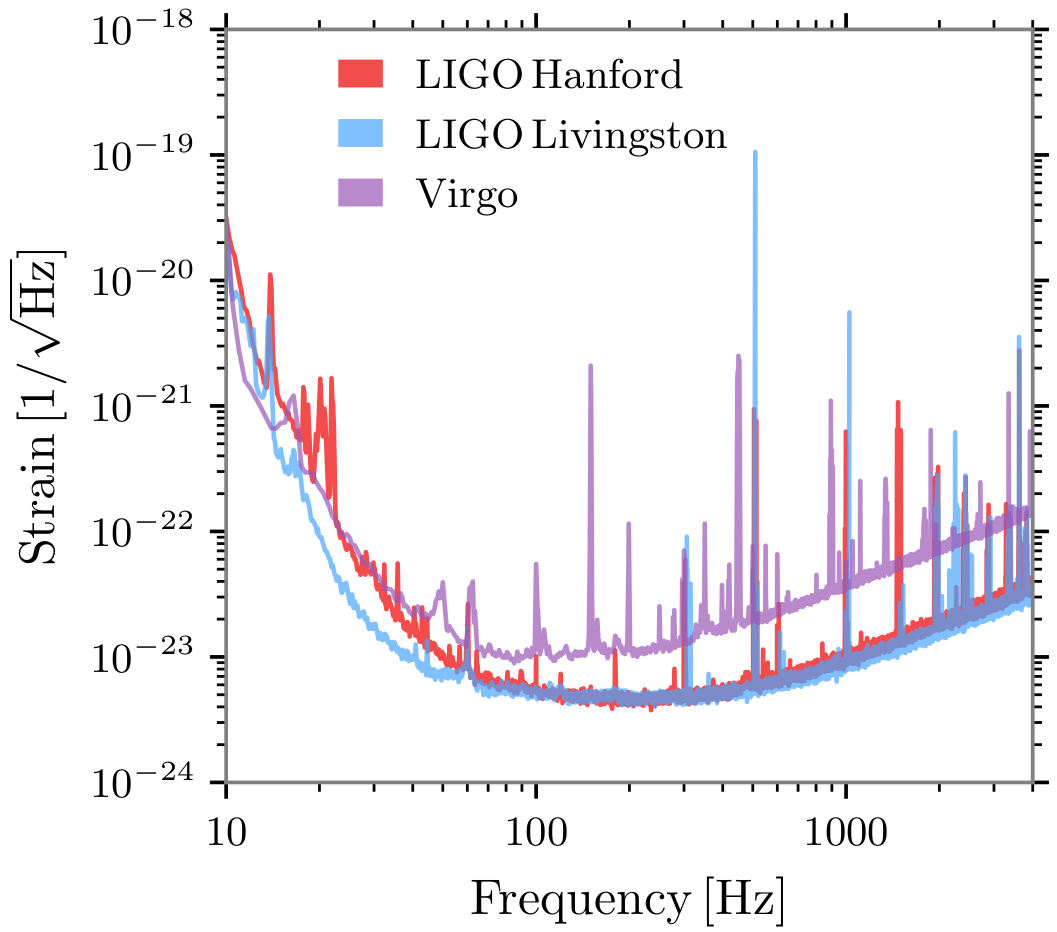
\includegraphics[width=\textwidth]{./images/sensitivity.png}
	\end{minipage}
	\hfill
	\begin{minipage}{.53\textwidth}
		\centering
		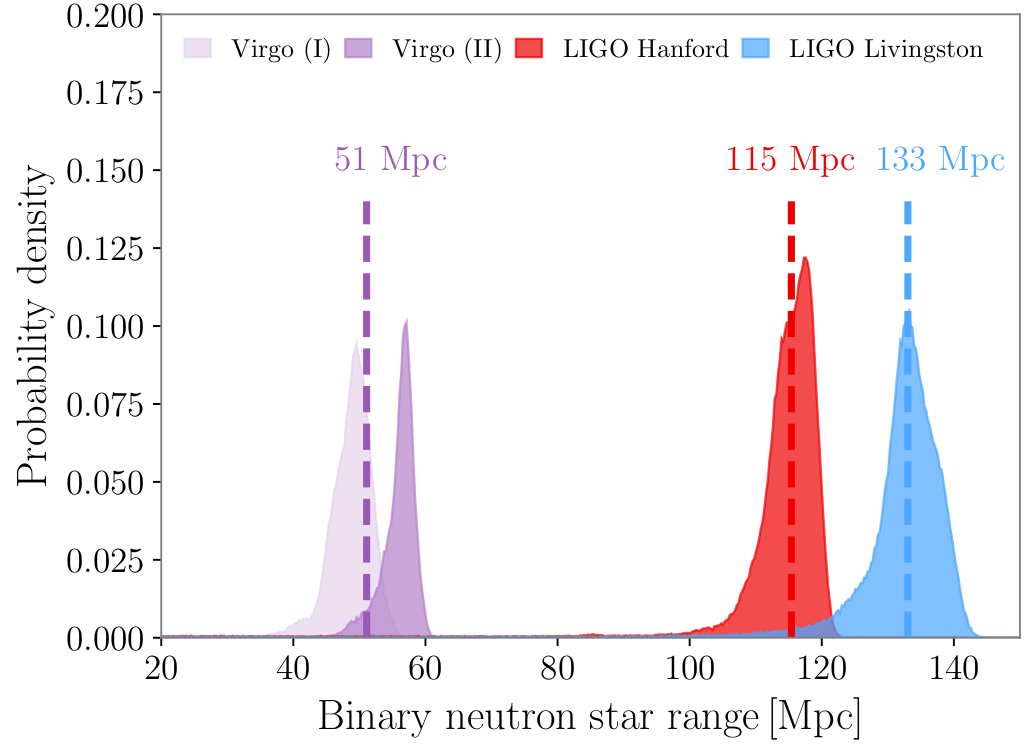
\includegraphics[width=1.02\textwidth]{./images/O3BNSrange.png}	
	\end{minipage}
	\caption{Sensitivity curves (\emph{left}) and binary neutron star observational probability density (\emph{right}) of the LIGO and Virgo interferometers during the third observing run O3. The lower sensitivity of Virgo for $\nu \gtrsim 150~\text{Hz}$ limits the observable volume, especially for the lighter sources like the binaries of neutron stars \cite{GWTC-3}.}\label{fig:O3sensitivity}
\end{figure}



\begin{figure}[h]
	\begin{minipage}{.49\textwidth}
		\centering
		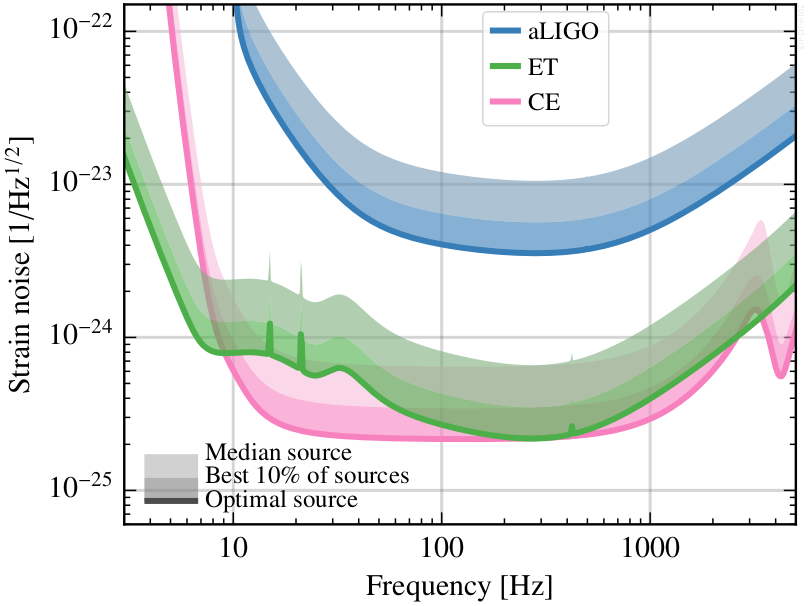
\includegraphics[width=\textwidth]{./images/ETsensitivity.png}
	\end{minipage}
	\hfill
	\begin{minipage}{.49\textwidth}
		\vspace{-2mm}
		\centering
		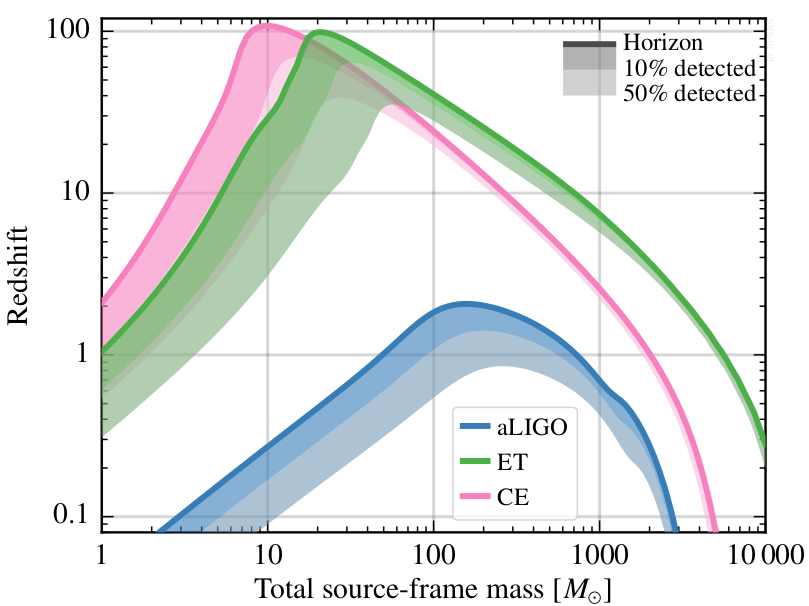
\includegraphics[width=1.02\textwidth]{./images/EThorizon.png}	
	\end{minipage}
	\caption{Example of the possible sensitivity curves (\emph{left}) and instrumental horizons (\emph{right}) of the planned third generation interferometers Einstein Telescope and Cosmic Explorer. Unlike the advanced LIGO interferometer, Einstein Telescope and Cosmic Explorer will detect binary black holes well-beyond redshift $z \sim 2$ \cite{EThorizonsensitivity}.}\label{fig:ETsensitivity}
\end{figure}


\paragraph{Sensitivity, biases and future perspectives}
According to Eq.\ \ref{eq:h}, the farther the sources are, the lower the amplitude of the gravitational wave that reaches the detector.  To have a quantitative comparison it is useful to use as proxy-source a binary neutron star: the limits on its equation of state impose that a single neutron star has at maximum a mass of $\sim 3~\msun$, therefore the binary chirp mass is well-defined and doesn't exceed $\mathcal{M} \sim 2.6 ~\msun$ \cite{NSreview}. Fig. \ref{fig:O3sensitivity} reports the sensitivity curves of the LIGO and Virgo interferometers and the end of the third observing run O3, highlighting how the worst sensitivity of Virgo at the high frequency (mainly caused by the photon shot noise) limits the maximum observable distance of the binary neutron star by a factor of 2 when compared to the performances of LIGO \cite{GWTC-3}.

In terms of binary black holes, a source like GW150914 that peaks at $\nu \sim 300~\text{Hz}$ could be observed by the LIGO interferometers with sensitivity of $h \sim 10^{-23}~ \text{Hz}^{-1/2}$ up to a luminosity distance of $d_L \sim 1.6~\text{Gpc}$: the binary can now be observed in a volume of space $\sim 64$ times bigger. The observable volume is maximum for binaries that merge close to the best sensitivity range at $\sim 100-200~\text{Hz}$, that, according to Eq.\ \ref{eq:nupeak} are likely binaries composed of heavy black holes with a total mass  $M_1+M_2 \sim 60-100~\msun$: the gravitational wave detectors are biased towards the observation of heavy binary black holes.


Third generation gravitational wave detectors, like the planned Einstein Telescope and Cosmic Explorer, will be at least one order of magnitude more sensible than advanced LIGO and Virgo at design sensitivity, allowing to probe binary compact object mergers beyond redshift $z \sim 2$. As shown in Fig.\ \ref{fig:ETsensitivity}, the maximum observable distance depends on source mass and interferometers' sensitivity, that ultimately depends on its design (Fig.\ \ref{fig:ETsensitivity} is only one of the proposed designs, but is representative of the goals of the project)  \cite{EThorizonsensitivity}. Again, Eq.\ \ref{eq:h} underlines how the detection improvement is mainly for binary black holes: their heavier mass produces stronger amplitude signals than binary neutron stars, making them visible even at high redshift.



\subsection{Observed distributions of mass and spin}\label{subsec:GWmassspin}

\paragraph{Merger rate densities and posterior distributions}
The parameter distributions of the observed gravitational wave sources are usually expressed either in terms of cumulative density functions (CDFs) or in terms of \emph{merger rate densities} (MRDs), the latter being the number of sources that merge in a co-moving volume and in a given time range. Both distributions are derived as posterior distribution functions (PDFs) $p(\theta)$ of some parameter $\theta$ in the framework of an hierarchical Bayesian analysis, that accounts for the observational biases and fits the hyper-parameters $\Lambda$ for the intrinsic population properties. From a theoretical perspective, the hyper-parameter fits are one of the most fundamental information to extract from the observations: their values can be directly compared with the predictions of the population-synthesis codes, discriminating between the different models proposed for the formation of the compact object merges \cite{GWTC-3_interpretation, BayesforGW}. \\

The astrophysical PDF of the source parameter $\theta$ is calculated averaging the prior distribution of the source $\pi(\theta|\Lambda)$ over the population hyper-parameters $\Lambda$

\begin{equation}\label{eq:posteriorMRD}
    p(\theta) = \int \pi(\theta|\Lambda)~p(\Lambda|\vec{d})~\rm d \Lambda
\end{equation}

The prior $\pi(\theta|\Lambda)$ is the intrinsic distribution of the source parameter $\theta$ for a given set of hyper-parameters $\Lambda$. The hyper-posterior $p(\Lambda|\vec{d})$ indicates the most probable values for the hyper-parameters $\Lambda$ given the observed data vector $\vec{d}$. Intuitively, the hyper-posterior could be a Gaussian that shifts and tightens around the true values of the hyper-parameters the more data are collected i.\ e.\ the more the data are representative of the population of interest.

To be more clear, it is possible to consider as an example a posterior distribution of the primary mass $p(M_1)$ similar to the one shown in the left-hand panel of Fig.\ \ref{fig:primarymassspectrum}. A reasonable choice for the prior could be a power-law (possibly related to the power-law of the initial mass functions of the stars \cite{Kroupa2001}) plus a Gaussian $\mathcal{N} (\mu,\sigma)$ centered in $\mu$ with dispersion $\sigma$ (to indicate possible over-densities) % lo so che ci sarebbe anche una massa minima per il modello vero, ma qui sto solo facendo un "esempio didattico" semplice

\begin{equation}\label{eq:priormassprimary}
    \pi(M_1|\alpha,\mu,\sigma) \propto M_1^{-\alpha}~\mathcal{N} (\mu,\sigma)
\end{equation}

The three hyper-parameters $\vec{\Lambda} = (\alpha,\mu,\sigma)$ will be then determined by the fit to the data. Since population-synthesis codes too can predict the intrinsic distribution of the primary masses $p(M_1)$, it is possible to reject the results and the corresponding underlying assumptions of the ones that, for instance, predict a Gaussian peak in a different position than the one obtained from the hyper-parameter fits.\\


According to Bayes theorem, the hyper-posterior $p(\Lambda|\vec{d})$ is proportional to the hyper-likelihood $\mathcal{L}(\vec{d}|\Lambda)$ an to the hyper-prior $\pi(\Lambda)$

\begin{equation}\label{eq:hyperposterior}
     p(\Lambda|\vec{d}) \propto~\mathcal{L}(\vec{d}|\Lambda)~\pi(\Lambda)
\end{equation}

The hyper-prior $\pi(\Lambda)$ indicates the prior beliefs on the hyper-parameters $\Lambda$ and usually is assumed to be uniform and non-informative. The hyper-likelihood $\mathcal{L}(\vec{d}|\Lambda)$ is the key quantity determined by the data and accounts for the observational biases. Assuming that the number of detected gravitational-waves $N_{\rm det}$ is related to the intrinsic number of events through a Poisson statistics, the hyper-likelihood can be modelled as

\begin{equation}\label{eq:hyperlikelihood}
    \mathcal{L}(\vec{d}, N_{\rm det}| \Lambda) \propto N^{N_{\rm det}}~e^{-N\xi(\Lambda)} ~\prod_{i=1}^{N_{\rm det}} \int \mathcal{L}(d_i|\theta)~\pi(\theta|\Lambda)~\rm d\theta
\end{equation}

The product $N^{N_{\rm det}}~e^{-N\xi(\Lambda)}$ encodes the information on the observational biases and detection efficiency. In fact, $N$ indicates the expected number of mergers over the observation period while $\xi(\Lambda)$ is the fraction of mergers that are detectable for the population characterized by hyper-parameters $\Lambda$. $N^{N_{\rm det}}~e^{-N\xi(\Lambda)}$ is strongly influenced by the dimension of the co-moving time-volume $\langle V\,T\rangle$ explored by the detector, namely the instrumental horizon integrated for the observation time.

The single-event likelihood $\mathcal{L}(d_i|\theta)$ is usually obtained via importance sampling from a default prior $\pi_{\rm def}(\pi)$. Therefore, the integral of the prior $\pi(\theta|\Lambda)$ over the single-event likelihood $\mathcal{L}(d_i|\theta)$ can be evaluated averaging over the posterior samples

\begin{equation}
   \int \mathcal{L}(d_i|\theta)~\pi(\theta|\Lambda)~\rm d\theta \approx \langle~ \frac{\pi(\theta|\Lambda)}{\pi_{\rm def}(\pi)}~\rangle
\end{equation}


\begin{figure}
	\begin{minipage}{.60\textwidth}
		\centering
		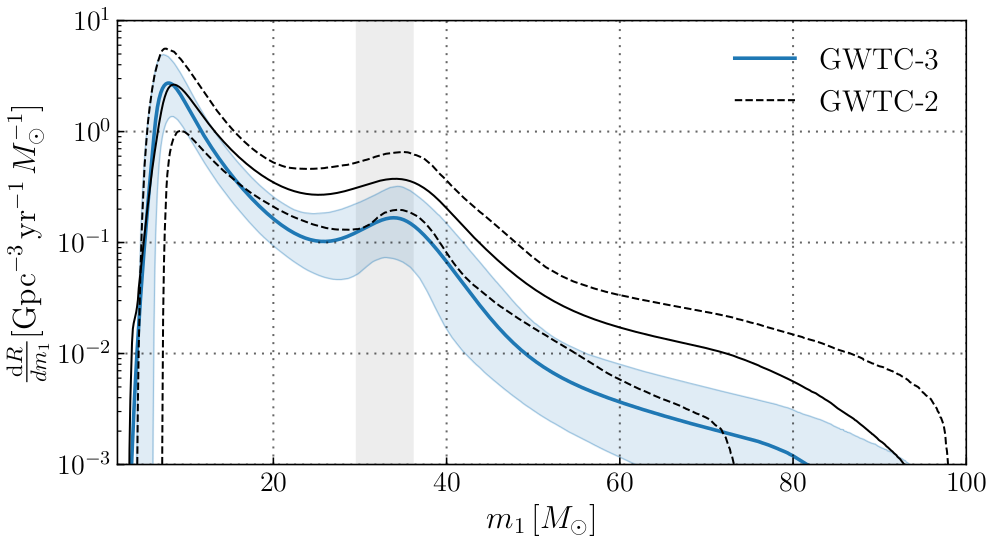
\includegraphics[width=\textwidth]{./images/MassMergerRate.png}
	\end{minipage}
	\hfill
	\begin{minipage}{.39\textwidth}
		\vspace{1mm}
		\centering
		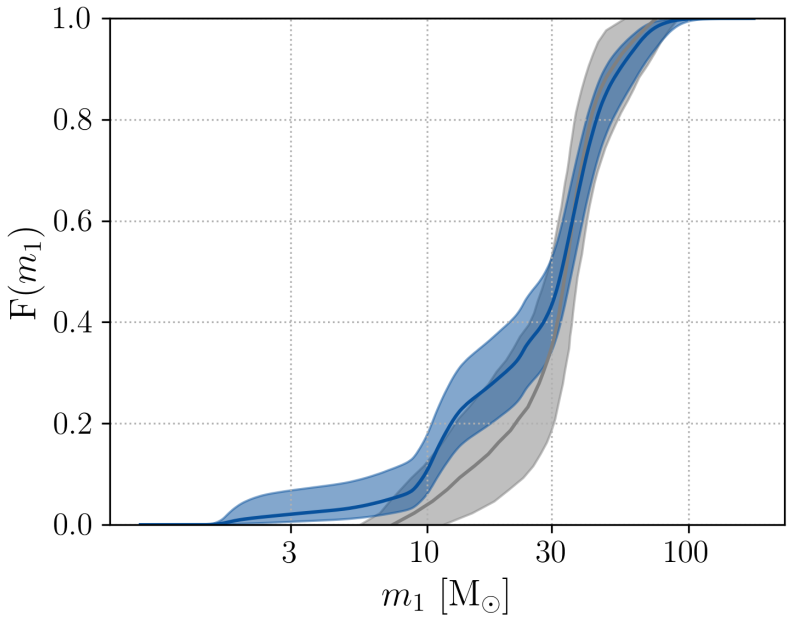
\includegraphics[width=\textwidth]{./images/MassCumulative.png}	
	\end{minipage}
	\caption{Differential merger rate density  (\emph{left}) and cumulative density function (\emph{right}) of the primary mass of the binary black holes detected with the gravitational waves. In blue the posterior distributions obtained with GWTC-3, in grey the ones obtained with GWTC-2. The thick solid lines denote the median values and are surrounded by the 90 \% credible intervals.The vertical grey band on the differential merger rate indicates the 90 \% credible interval for the mean of the Gaussian peak \cite{GWTC-3_interpretation}.}\label{fig:primarymassspectrum}
\end{figure}


\paragraph{Primary mass spectrum}
For each binary source, the primary mass is defined as the most massive compact object. The differential merger rate density of the primary mass observed at the end of O3b is a power-law with slope $\alpha = 3.5_{-0.56}^{+0.6}$ with a Gaussian peak centered in $M_{\rm 1,\mu} = 34_{-4.0}^{+2.6}~ \msun$. GWTC-3 contains more low-mass system than GWTC-2, causing a steeper decline in the power law at higher masses and reducing the mass of the 99th percentile, now at $\sim 44~\msun$ and not at $\sim 60~\msun$ as it was in GWTC-2. There are strong over-densities at $\sim 10~\msun$ and $\sim 35~\msun$ that may reflect properties of the astrophysical environment but that are still under investigation.

Even though the region $\gtrsim 70~\msun$ is still weakly explored, there is no strong evidence for or against an upper mass gap, at least up to $\sim 75~\msun$. Still, a similar finding challenges the existence of the pair-instability mass gap ($\sim 60 - 120~\msun$ \cite{spera2017_pisnSNe}): either the single stellar evolution models need to be corrected \cite{MassGapStellarEvo_Costa2021} or the formation in dynamically active environments is required \cite{Rastello2021_dynamics}. On the other hand, there is still mild support for a lower-mass gap between $\sim 3~\msun$ and $\sim 5~\msun$, potentially due to the physics of core-collapse supernovae and in agreement with the dearth of compact objects observed in nearby X-ray binaries \cite{massgapreal_ozel2010}.




\paragraph{Spin distribution}
At the end of the third observing run, the black hole population exhibits a preference for low-spinning black holes $\chi \lesssim 0.4$, with a peak distribution at $\chi \sim 0.2$ and a long tail at higher values. Separate analysis of the fastest ($\chi_A$) and slowest ($\chi_B$) spinning components of the binary revealed that the rapid-spinning components are still quite slow $\chi_A \sim 0.4$ while the slow-spinning ones are concentrated below $\chi_B \sim 0.2$, as expected. Posterior distributions for the spin magnitudes are shown in Fig.\ \ref{fig:spinmagnitude}.

% ho un po' riaggiustato visto che dicevi che non ti era del tutto chiaro
As shown in the left-hand panel of Fig.\ \ref{fig:spineffective}, the effective spin parameter $\chi_{eff}$ distribution is still consistent with a Gaussian centered in $\chi_{eff, \mu} = 0.06_{-0.05}^{+0.04}$ with a peak still compatible with $\chi_{eff} = 0$, indicating either very low spin magnitudes or spins misaligned with the orbital angular momentum. In particular, the distribution extends to negative effective spins $\chi_{eff} < 0$, suggesting the existence of polar angle tilts $\theta \geq 90^\circ $ i.\ e.\ black holes anti-aligned with the orbital angular momentum that likely formed in dynamically active environments. This evolutionary scenario is consistent also with the flatter and more isotropic-oriented distribution of the tilt angles shown in the right-hand panel of Fig.\ \ref{fig:spineffective}. 



\begin{figure}[h!]
	\begin{minipage}{.49\textwidth}
		\centering
		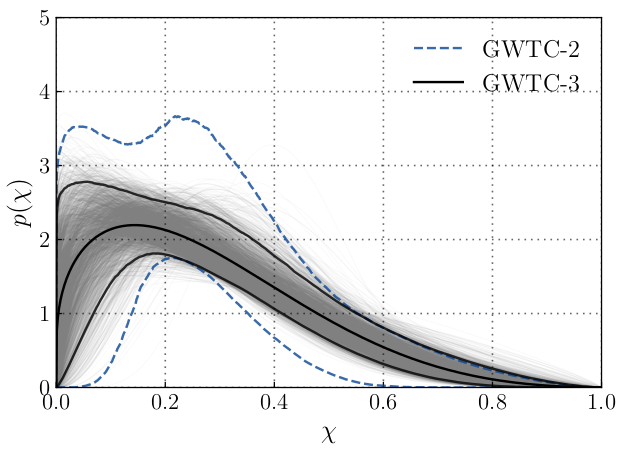
\includegraphics[width=\textwidth]{./images/spinmagnitude.png}
	\end{minipage}
	\hfill
	\begin{minipage}{.49\textwidth}
		\vspace{0.8mm}
		\centering
		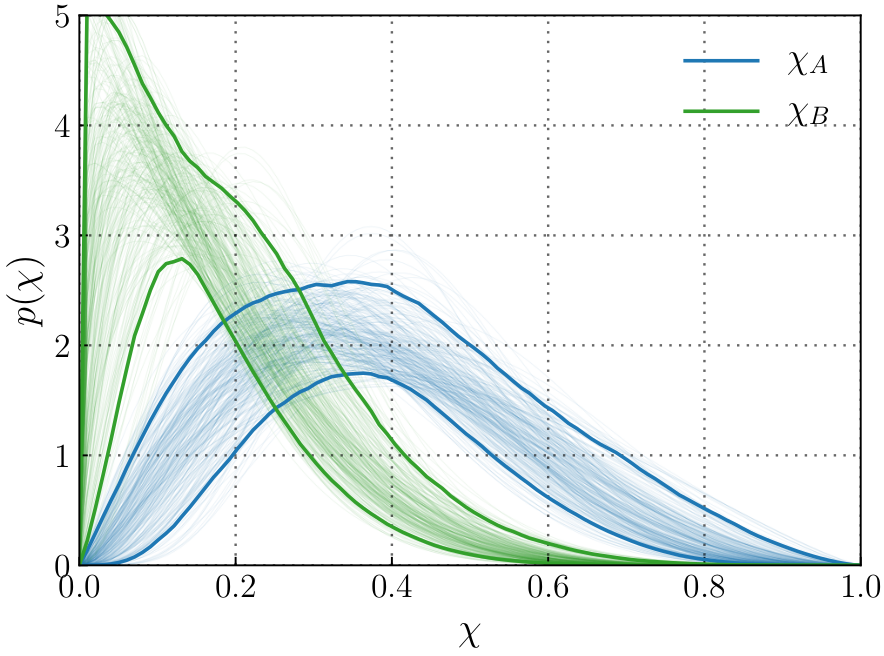
\includegraphics[width=0.975\textwidth]{./images/spinmagnitudehighlow.png}	
	\end{minipage}
	\caption{\emph{Left:} Spin magnitude ($\chi$) posterior distribution of all the merging black holes in GWTC-3 (gray) compared to the 90 \% credible intervals for GWTC-2 (in blue). \emph{Right:} Separate posterior distributions within 90 \% credible bounds of the fastest ($\chi_A$, in blue) and slowest ($\chi_B$, in green) black holes in the binary. The new observations indicate a preference for slow-spinning black holes $\chi \lesssim 0.4$, with a fast-spinning component still rather slow $\chi_A \sim 0.4$ \cite{GWTC-3_interpretation}} \label{fig:spinmagnitude}
\end{figure}


\begin{figure}[h!]
	\begin{minipage}{.49\textwidth}
		\centering
		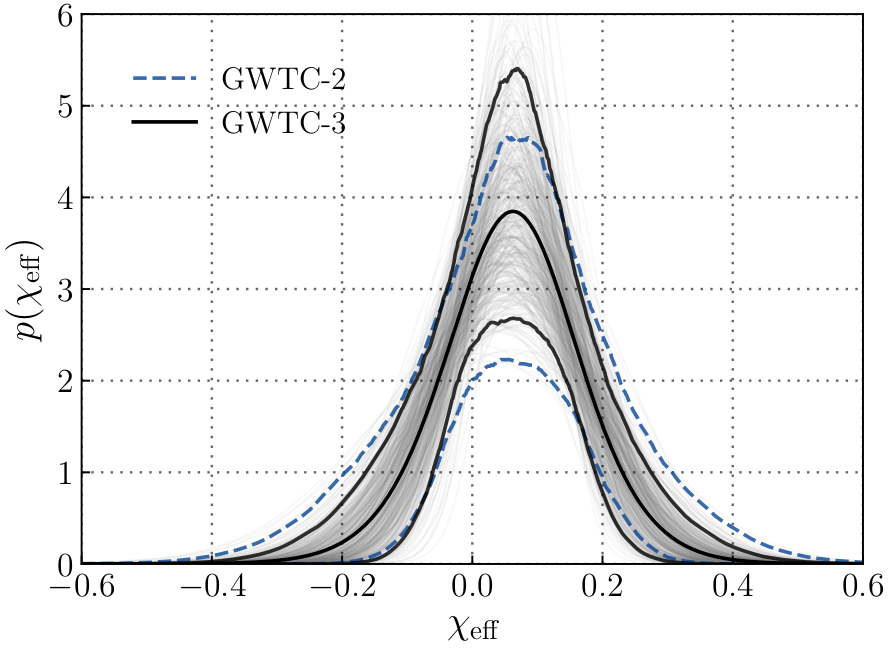
\includegraphics[width=\textwidth]{./images/spineff.png}
	\end{minipage}
	\hfill
	\begin{minipage}{.49\textwidth}
		\vspace{-1mm}
		\centering
		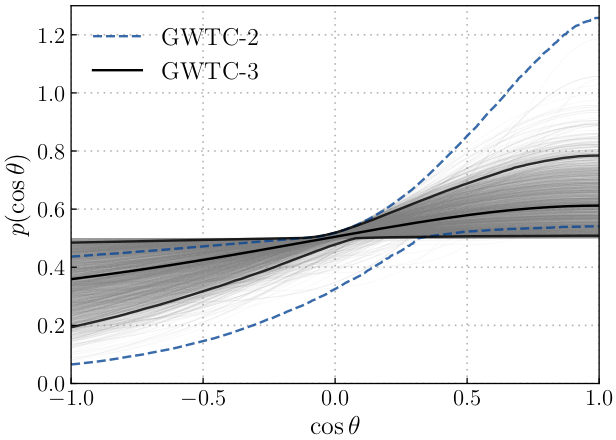
\includegraphics[width=0.96\textwidth]{./images/spinorientation.png}	
	\end{minipage}
	\caption{\emph{Left:} Gaussian posteriors of the effective spin $\chi_{eff}$ of all the merging black holes in GWTC-3 (gray) compared to the 90 \% credible intervals for GWTC-2 (blue). \emph{Right:} Posterior distribution of the polar angle $\theta$ of all the merging black holes in GWTC-3 (gray) compared to the 90 \% credible intervals in GWTC-2 (blue) \cite{GWTC-3_interpretation}.} \label{fig:spineffective}
\end{figure}

\begin{figure}[h!]
	\begin{minipage}{.49\textwidth}
		\centering
		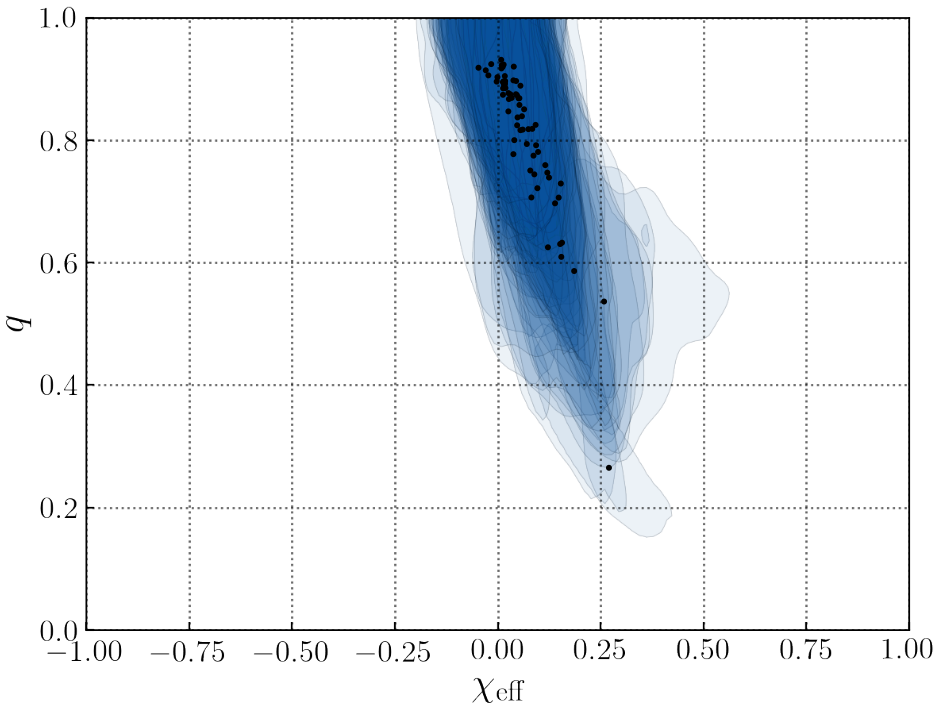
\includegraphics[width=\textwidth]{./images/spinmassratio.png}
	\end{minipage}
	\hfill
	\begin{minipage}{.49\textwidth}
		%\vspace{-2mm}
		\centering
		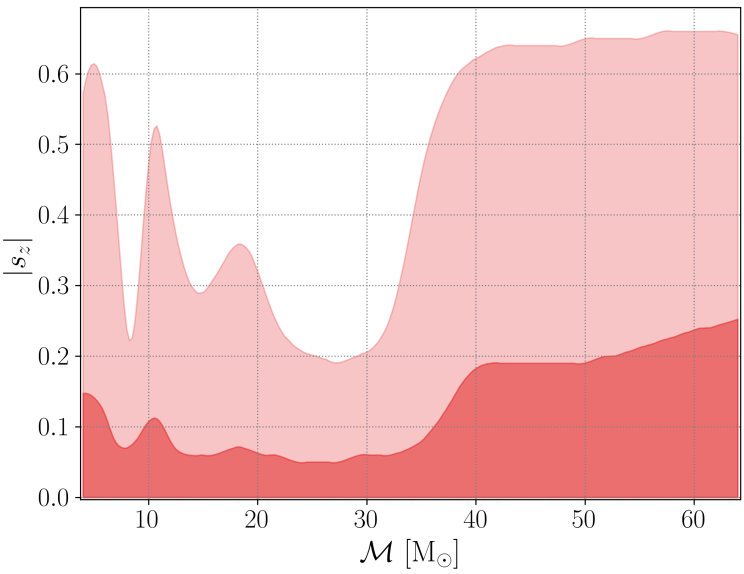
\includegraphics[width=0.95\textwidth]{./images/spinchirpmass.png}	
	\end{minipage}
	\caption{\emph{Left:} Effective spin $\chi_{eff}$ anti-correlating with the mass ratio $q$. Black points mark the median of the PDF obtained using an informed prior where mean and standard deviation of the Gaussian posterior of $\chi_{eff}$ were allowed to evolve with $q$. Blue shaded areas indicate the 90 \% credible intervals for each median point. \emph{Right:} Spin component parallel or anti-parallel to the orbital angular momentum vector $\vec{s}_z$ as a function of the binary chirp mass. Light (dark) shaded areas indicate 90 \% (50 \%) credible intervals \cite{GWTC-3_interpretation}.}\label{fig:spincorrelations}
\end{figure}



Data from GWTC-3 exhibit a mild anti-correlation between the effective spin parameter $\chi_{eff}$ and the mass ratio $q$, as shown in the left-hand panel of Fig.\ \ref{fig:spincorrelations}. If confirmed, the anti-correlation would challenge the usual evolutionary pathways for binary black hole progenitors, indicating that field binaries formed with $q \sim 1$ do not have spins aligned with the orbital angular momentum ($\chi_{eff} \sim 1$),  because either the tides and mass transfer are not so efficient or there is some additional and yet unknown effect, like a third-body perturbation \cite{misalignedbinary}.


So far the LVC analysis has been carried out assuming the same spin distribution at all masses, even though the low-mass binaries dominate the sample and seven high-mass binaries make up $\sim 70 \%$ of the moderate spins. A more refined analysis compared the spin component aligned with the orbital angular momentum $|s_z|$ with the chirp mass of each binary. The result is shown in the right-hand panel of Fig.\ \ref{fig:spincorrelations}. All the binaries are consistent with spins misaligned with the orbital angular momentum ($|s_z| = 0$) even tough there are over-densities in the chirp mass distribution: if confirmed by further detections it would challenge the correlations predicted by the hierarchical formation scenario. The large spread of the high-mass binaries $\mathcal{M} \gtrsim 30~\msun$ with respect to the low-mass ones is consistent with having a large number of detections at low masses and fewer at high masses: at the moment it is not possible to reject or confirm an aligned spin magnitude dependence with the chirp mass.











\section{X-ray binaries}\label{sec:Xraybinaries}

\subsection{X-ray binaries hosting a black hole}\label{subsec:XraybinariesSED}

\paragraph{The best way to observe a black hole}
X-ray binaries that host a black hole and a massive star are currently the best observational candidates as binary black hole progenitors: not only such systems are already in a binary configuration but the accretion onto the compact object powers an X-ray emission that allows us to observe them \cite{Xbinaries_massmeasure}. The possibility to observe them is precisely the key property of X-ray binaries: even though $\sim 70 \%$ of massive stars are born in binary systems \cite{Sana2012}, most black holes are quiescent and can be observed only with accurate measurements of their radial velocity or proper motions \cite{BHnoninteracting_Giesers2018}. Isolated black holes, that could dynamically exchange with a binary, are even more difficult to observe and currently the best detection technique for them is microlensing \cite{BHmicrolensing}.

\paragraph{LMXBs and HMXBs}
The mass of the non-degenerate donor star and the type of accretion determine two sub-classes of X-ray binaries hosting a black hole: low-Mass X-ray binaries (LMXBs) and high-mass X-ray binaries (HMXBs). LMXBs typically host low-mass stars $\lesssim 2-3~\msun$ that fill their Roche lobe. In contrast, HMXB  donors are more massive stars $\gtrsim 5~\msun$ that typically do not fill their Roche lobe but become wind-fed systems. Up-to-date, about $\sim 30$ X-ray binaries are estimated to host a black hole \cite{HMXBH_spins2021}.

\paragraph{Spectral energy distribution in the X-rays}
The X-ray spectral energy distribution of an X-ray binary is dominated by the emission of the accretion disk surrounding the compact object. A classic Shakura-Sunyaev accretion disk around a stellar-sized compact object emits most of its photons in the UV/soft X-ray regime $\sim 10^{2}-10^{4}$ keV with an X-ray luminosity $L_X \gtrsim 10^{37}~\text{erg s}^{-1}$, has an effective radiation temperature of $\sim 10^{7}-10^{8}~K$ and produces a thermal multi-color black-body continuum \cite{S&S1973_accretiondisk}. Usually, accretion disks are surrounded by a corona of hot thermal electrons: photons in the low energy tail of the disk thermal emission (soft optical/UV) that encounter the corona suffer multiple inverse Compton scatterings (i.\ e.\ suffer a thermal Comptonization) and are re-emitted in the form of a hard X-ray power-law spectrum. Part of the X-ray power-law radiation is directly emitted towards the observer at infinity but another part is re-emitted back to the accretion disk, reprocessed by it and eventually reflected at the infinity. 
 
The X-ray photons reprocessed by the corona are more energetic than the ones originally produced in the accretion disk and see the disk as a slab of cold gas, interacting with it mainly through Compton scattering and photoelectric absorption followed by fluorescent line emissions. On the one hand, the energy dependence of the photoelectric absorption favours the absorption of the soft X-rays, causing a down-scaling in the corresponding region of the reflected continuum. One other hand, the hard X-rays are Compton-scattered back, thus reflected towards the observer at the infinity, except for the ones more energetic than $\sim 20-30$ keV, which suffer Compton recoil. Overall, the X-ray continuum due to reflection is characterized by a hump at $\sim 20$ keV and by the fluorescent lines emitted by the ionized heavy elements, mainly iron. The 6.4 keV line of the Fe K$\alpha$ line is the strongest fluorescent line and is caused by the absorption of an incident photon with energy larger than 7.1 keV, as shown in the right-hand panel of Fig. \ref{fig:accretiondisk}.

The X-ray continuum seen by an observer at infinity can be divided into soft and hard X-ray regimes, respectively below or above 10 keV. The soft X-ray spectrum is dominated by the thermal continuum of the disk and exhibits a multi-color black body shape peaked at $\sim 2$ keV. The hard X-ray spectrum is determined by the radiation reprocessed by the hot corona: the hard power-law of the photons directly emitted from the corona is modulated by the hump at $\sim 20$ keV and the fluorescence emission lines caused by the additional reflection on the accretion disk, as shown in the left-hand panel of Fig. \ref{fig:accretiondisk} \cite{FeKalphaline_Fabian2000}.


\begin{figure}
	\begin{minipage}{.58\textwidth}
		\centering
		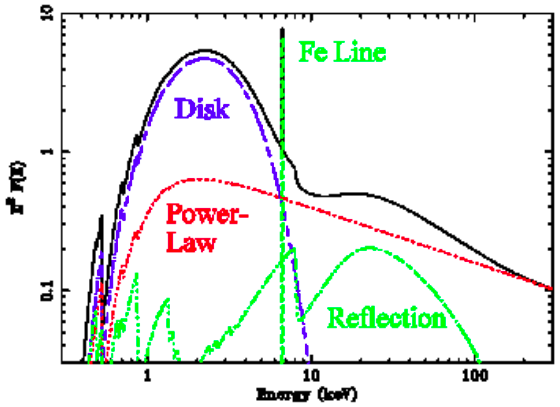
\includegraphics[width=\textwidth]{./images/accretiondiskSED.png}
	\end{minipage}
	\hfill
	\begin{minipage}{.42\textwidth}
		%\vspace{-2mm}
		\centering
		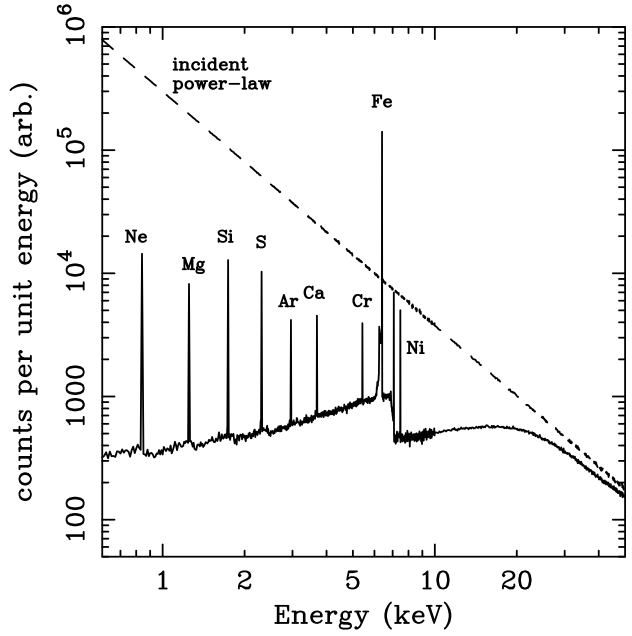
\includegraphics[width=\textwidth]{./images/accretiondiskFeKalphaline.png}	
	\end{minipage}
	\caption{\emph{Left:} Sketch of the dominant components in the spectral energy distribution of an X-ray binary. In the soft X-rays, the emission is dominated by the thermal continuum of the disk, visible as a multi-color black-body peaked at $\sim 2$ keV. In the hard X-rays, the radiation reprocessed by the corona is either directly emitted towards the observer as a power-law or is reflected by the disk, causing a hump at $\sim 20$ keV and the strong fluorescent Fe K$\alpha$ line at $6.4$ keV. Credit: J. Miller \emph{Right:} Montecarlo simulation of the X-ray spectrum reflected by a cold slab of gas. An incident power-law radiation (dashed line) is damped in the soft X-rays, exhibiting strong fluorescent lines and a hump before the cut-off due to Compton recoil \cite{FeKalphaline_Fabian2000}.}\label{fig:accretiondisk}
\end{figure}

\subsection{Measuring the properties of  X-ray binaries}\label{subsec:Xraymeasure}
\paragraph{Masses, period and inclination}
Inspection of the radial velocity and X-ray light curves provides essential information to characterize the orbital properties of X-ray binaries. The orbital period can directly be obtained from the periodicity of the light and velocity curves and often is the most-accurate orbital parameter. The mass estimate of the compact object is less precise and relies on the determination of other uncertain quantities, like the companion mass, binary mass ratio, inclination and distance.

The dynamical method is the most robust and common procedure to determine the mass of an object in a binary system. Its application is limited to the systems that satisfy three conditions: the companion star is visible in the optical/near-infrared band, single spectral lines can be identified in its optical/near-infrared spectrum (resolving power $\lambda/\Delta \lambda \gtrsim 1500$), at least one photospheric absorption line can be used as a proxy for the orbital motion. Therefore, the dynamical method cannot be applied to distant X-ray binaries (not enough resolving power), to systems with a companion not visible in the optical/near-infrared band and, most importantly, to systems subject to outbursts or strong stellar winds. These limitations prevent the application of the dynamical mass determination to many HMXBs. For instance, as explained in Sec.\ \ref{sec:WRBHobserved}, the strong winds of the  Wolf-Rayet star coupled with the X-ray variability of the compact object caused the revision of several important dynamical mass measurements in the Wolf -Rayet -- black hole binaries \cite{ICX10X-1_Laycock2015_revisited}.

Alternative techniques for the mass measurement are available but still require a good calibration, as for the case of the scaling relations with the X-ray spectral and timing properties in presence of quasi-periodic oscillations \cite{Xbinaries_massfromXtiming}.\\

According to the dynamical method, the spectral lines that trace the orbital motion are used to build the velocity curves and extract the orbital period $P_{orb}$ and the radial velocity semi-amplitude $K_c$ of the companion star. Kepler's third law corrects the measures for the inclination angle $i$ and the mass ratio $q=M_c/M_{\rm BH}$ and couples them into the \emph{mass function} $f(M)$: a non-linear expression relating the masses of the companion star $M_c$ and of the compact object $M_{\rm BH}$:

\begin{equation}\label{eq:massfunction}
	f(M) = \frac{K_c^3 P_{\rm orb}}{2 \pi G} = \frac{M_{\rm BH}^3 \sin^3 i}{(M_{\rm BH} + M_c)^2} = \frac{M_{\rm BH}^3 \sin^3 i}{(1+q)^2}
\end{equation}

The above formula is for a circular binary: a reasonable assumption for a system that likely already had time to circularize, given that its X-ray emission is the result of a mass-transfer process. Eventually, the mass of the black hole in the binary can be determined with further assumptions and measurements on the mass ratio $q$ (or, alternatively, on the companion mass $M_c$) and on the inclination of the system $i$.\\

The mass ratio can be determined assuming a spherically symmetric star that fills its Roche lobe in a tidally locked system. Under these conditions, the rotational broadening ($V \sin i$) of the absorption lines in the stellar photosphere can be related to the mass ratio $q$ of the system \cite{Xbinaries_qmeasure}

\begin{equation}\label{eq:qmeasure}
	\frac{V \sin i}{K_c} \sim 0.462~q^{1/3} (1+q)^{2/3} 
\end{equation}

The measurement of $q$ is not always feasible and usually leads to under-estimate its value. The main uncertainty arises from the assumption of spherical symmetry in a Roche lobe filling system that, on the contrary, has tidal distortions. Moreover, the rotational broadening is usually of $\sim 30-120~\text{km s}^{-1}$ and requires a very large resolving power $\lambda/\Delta \lambda \gtrsim 5000$ to be measured, limiting the determination of $q$ only to the nearest binaries. 

For many systems, including the HMXBs that are not filling their Roche lobe, the mass function is not calculated with the mass ratio but with the companion mass. Fits on the stellar spectrum or mass-luminosity relations can provide the mass of the companion star. Usually the mass-luminosity relations are empirically obtained either by calibrations on synthetic spectra based on single stellar evolution models or by extrapolating the star properties from their position in the color-magnitude diagram (see Sec.\ \ref{subsec:massWR} for an example of a mass-luminosity relation for the Wolf-Rayet stars). The methodology requires a good modelling of stellar photospheres and optical/infrared emissions. However, strong winds and mass transfer events that expose the inner layers of the star or super-Eddington accretion onto the compact object may change the optical/infrared properties of the X-ray binary, leading to an uncertain estimate of the mass of the non-degenerate star \cite{superEddingtonaccBH_Ambrosi2018}. 

The inclination angle $i$ is usually obtained fitting the optical/near-infrared light curves with synthetic ellipsoidal models. Assuming that the companion star is filling its Roche lobe, tidal deformations of the star surface are expected to modulate the light curve profile and the amplitude of the modulation can be linked to the inclination angle. The light curve modulation can be affected by many sources of error (outburst, winds, etc.) and requires a very complex modeling, resulting in inaccurate determinations of the inclination angle. A similar, uncertain, result can be obtained also assuming that the inclination of the black hole high energy jet is the same of the binary: observations on the MAXI J1820+070 X-binary showed that spin-orbit misalignments can be $\gtrsim 40^{\circ}$ \cite{BHspinmisaligned_2022}. Unless the system is an eclipsing binary, its inclination angle is poorly constrained and, given the cubic dependence in the mass function of Eq.\ \ref{eq:massfunction}, provides the biggest source of uncertainty in the black holes mass determination \cite{Xbinaries_massmeasure}.\\


HMXBs usually do not fill their Roche lobe and power the accretion through strong stellar winds: not only the method just described would provide very uncertain determinations for the inclination angle and companion mass but it would result in a very imprecise measure of the black hole mass. Therefore, the mass of the compact object in HMXBs is usually the result of a multi-parametric fit to the radial velocity curve and to the optical/near-infrared and X-ray light curves. The distance of the source is one of the parameters included in the multi-parametric model and the fit result is very sensible to it. For instance, recent radio astrometric distance measurements re-defined Cyg X-1 as a system hosting an O-type star of $\sim 40~\msun$ with a black hole of $\sim 21~\msun$, making it the most massive black hole detected so far in an X-ray binary \cite{cygnusx1}.




\paragraph{Spin}
Two techniques are generally used to measure the spin of black holes and require a fit to the X-ray spectrum of the accretion disk, either on the continuum or on the Fe K$\alpha$ lines (see Sec.\ \ref{subsec:XraybinariesSED} for a more detailed description of the X-ray spectral energy distribution). Both methods assume a geometrically thin and radiatively efficient disk, with emission that terminates at the innermost stable circular orbit (ISCO) \cite{Xbinaries_spinBHmeasure}.\\

The Fe K$\alpha$ line at 6.4 keV is a very strong fluorescent line produced by the X-ray radiation reflected from the accretion disk. In principle the line is very narrow but it is broadened by the Doppler effect, due to the disk rotation, and by the gravitational redshift, due to the vicinity to the black hole. Fast spinning Kerr black holes have an ISCO that is both closer to the black hole and more rapidly rotating, enhancing the gravitational redshift and the Doppler shift, respectively. As shown in the left-hand panel of Fig.\ \ref{fig:spinmeasure}, the spin of the black hole can be reconstructed by carefully fitting the broadening of the Fe K$\alpha$ line in the reflected X-ray spectrum.

The fit to the reflection spectrum has the great advantage of being a \textit{relative} measurement. Moreover, the spin determination can be carried out without knowing a priori the black hole mass, its distance and accretion rate, allowing the spins to be inferred in many systems with poorly constrained black hole masses \cite{HMXBH_spins2021}. On the contrary, the emissivity and ionization of the disk need to be already modeled to provide a good fit. Reflection spectra are also very sensitive to the inner disk inclination, although this information can be extracted by the same fit used for the Fe K$\alpha$ line.\\

Spin determination through the fit of the hard continuum relies again on having an ISCO of the disk closer to the black hole for high spin values. The thermal emission of the disk can be modeled as a multi-color black-body, where each anulus emits as a thermal black-body with radiation temperature $T \propto r^{-3/4}$ hotter for anuli closer to the black hole. Fast rotating black holes have accretion disks with ISCO very close to the black horizon that, being hotter, shift the peak of the multi-color emission towards higher energies: fitting the absolute shift in the flux emitted in the hard X-rays results in the spin determination, as shown in the right-hand panel of Fig.\ \ref{fig:spinmeasure}.

The method has many drawbacks, the main one being its necessity to fit the \textit{absolute} flux shift in a region where the emitted flux is strongly influenced also by the hard power-law emitted by the corona (see the left-hand panel of Fig.\ \ref{fig:accretiondisk} for a comparison): the choice of the hard component strongly impacts the spin value. Further sources of uncertainty come from the a priori knowledge of the inner disk inclination (in particular, the delicate assumption of spin and orbital angular momentum aligned \cite{BHspinmisaligned_2022}), atmospheric scattering corrections and, most importantly, mass and distance of the black hole, required to have an accurate model for the absolute flux emitted by the disk \cite{Xbinaries_spinBHmeasure}.


\begin{figure}
	\begin{minipage}{.48\textwidth}
		\centering
		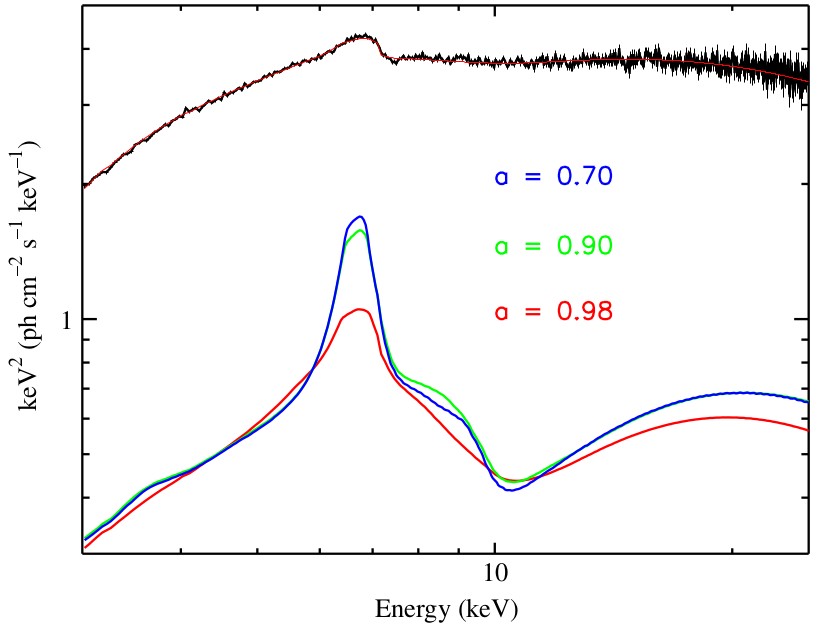
\includegraphics[width=\textwidth]{./images/spinreflection.png}
	\end{minipage}
	\hfill
	\begin{minipage}{.49\textwidth}
		%\vspace{-2mm}
		\centering
		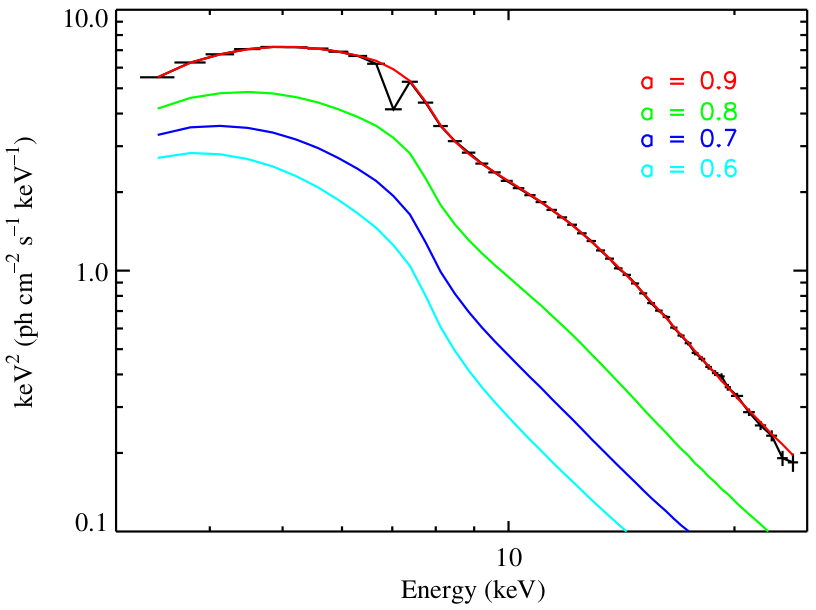
\includegraphics[width=\textwidth]{./images/spincontinuum.png}	
	\end{minipage}
	\caption{Example of the black hole spin measurement from fits to the Fe K$\alpha$ line (\emph{left}) or to the X-ray hard continuum (\emph{right}) of the candidate X-ray binary GRS 1915+ 105. The Fe K$\alpha$ fluorescent line causes the absorption at $\sim 7$ keV in the right-hand panel and results in a strong, broadened emission centered at 6.4 keV in the left-hand panel. The spectrum on the left is obtained with \textit{NuStar} while the one on the right with \textit{RXTE} \cite{GSR1915_lowhardXstate}.}\label{fig:spinmeasure}
\end{figure}


\section{Tensions in the underlying populations}\label{sec:tensionmassspin2021}
Up-to-date, one of the most detailed analysis of the mass and spin distribution of the underlying binary black hole populations was carried out in 2021 by Fishbach \& Kalogera \cite{HMXBH_spins2021} and compared the data of 44 binary black holes of the GWTC-2 catalogue with the only X-ray binaries with a reliable mass or spin measurement: 3 HMXBs and 29 LMXBs, of which only 20 have a reliable mass (see Sec.\ \ref{subsec:Xraymeasure} for a discussion on the main uncertainties in the X-ray parameter estimation). This study included as HMXBs the X-ray binaries with O-type donor star LMC X-1, M33 X-7 and Cyg X-1, excluding the Wolf-Rayet -- black hole binaries like NGC 300 X-1 or IC 10 X-1 because they have a less reliable mass measurements \cite{ICX10X-1_Laycock2015_revisited} (see the discussion in Sec.\ \ref{sec:WRBHobserved}). Even though the binary black hole sample is limited to GWTC-2 \cite{GWTC-2}, it is reasonable to expect that the same conclusions can be obtained using the GWTC-3 data, as discussed in Sec.\ \ref{subsec:GWmassspin}. In contrast, the limited sample of X-ray binaries with reliable mass and spin measurements causes the largest uncertainties.


\begin{figure}[h]
	\begin{minipage}{.49\textwidth}
		\centering
		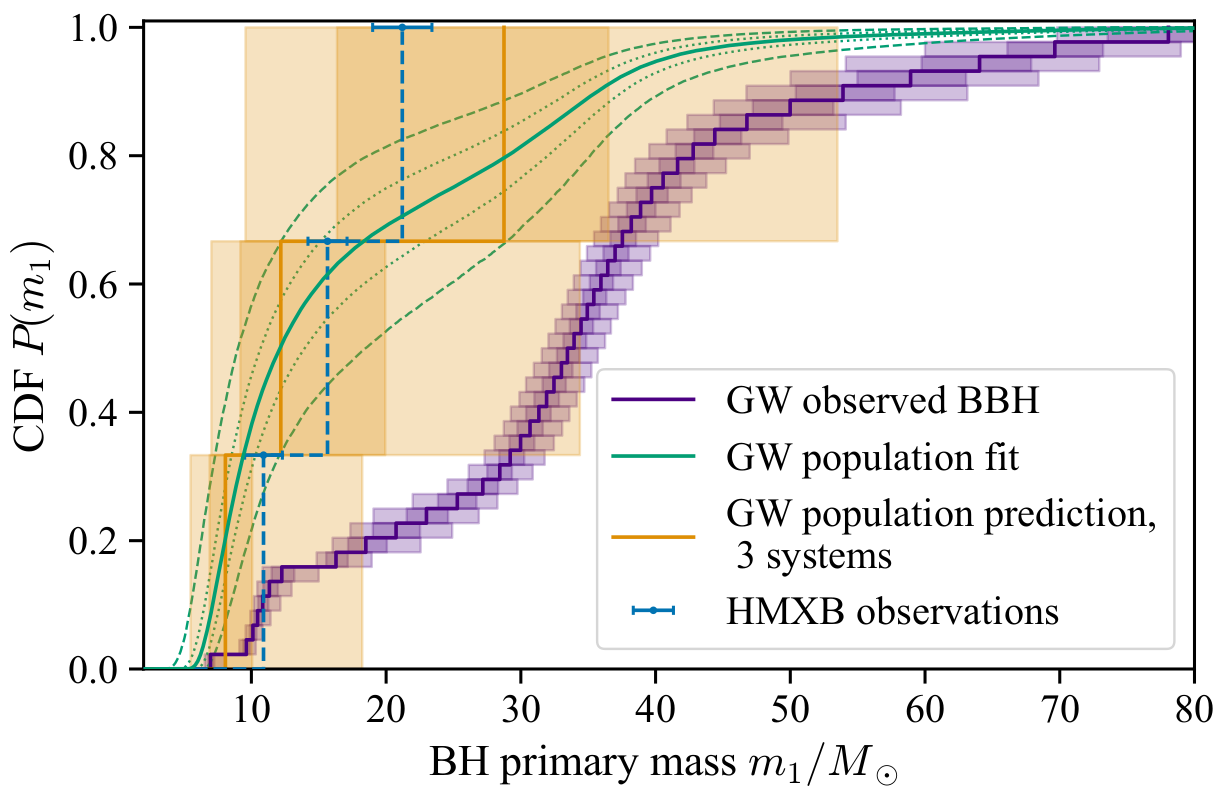
\includegraphics[width=\textwidth]{./images/tensionHMXBHmass.png}
	\end{minipage}
	\hfill
	\begin{minipage}{.49\textwidth}
		\vspace{.5mm}
		\centering
		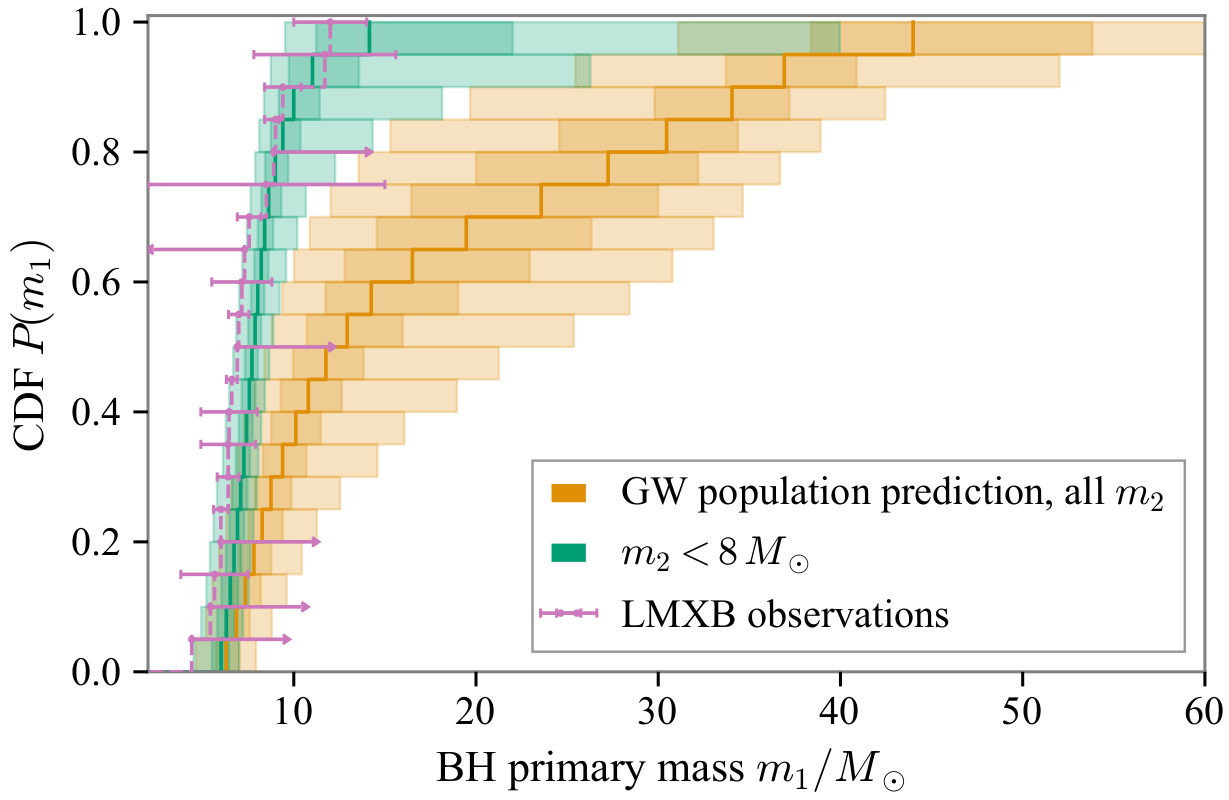
\includegraphics[width=\textwidth]{./images/tensionLMXBHmass.png}	
	\end{minipage}
	\caption{Observed cumulative distribution function (CDF) of the observed HMXBs (blue, \emph{left-hand} panel) and LMXBs (pink, \emph{right-hand} panel) compared with the CDFs (orange bands) expected if the X-ray binaries share the same primary black hole mass distribution as the primaries of the LVC binary black holes, once it is corrected for selection effects (green line). In the left-hand panel, the purple bands show the original observed CDF for binary black holes not yet corrected for observational effects. In the right-hand panel, the green bands show the CDF extracted from the sub-sample of the LVC binary black holes with secondary mass $< 8~\msun$. Dark (light) shaded areas delimit 50 \% (90 \%) credible intervals \cite{HMXBH_spins2021}}.\label{fig:tensionmass}
\end{figure}

\subsection{Similarities in the mass distribution}
The mass distribution of the primary (more massive) black hole of the LVC binary black holes seems compatible with the mass distribution of the black holes in LMXBs and HMXBs, once the corrections for gravitational wave selection effects and similar mass pairing are taken into account. If confirmed, the relation would indicate that X-ray binaries hosting a black hole could be the progenitors of the binary black hole mergers. However, the small sample of X-ray binaries with reliable mass measurements ($\sim 20$) is affected by a large Poisson uncertainty, possibly hiding inconsistencies in the underlying populations. Moreover, observational selection effects on the X-ray binaries are not accounted for and may further change the degree of consistency. \\

The left- and right-hand panel in Fig.\ \ref{fig:tensionmass} show the agreement between the cumulative distribution functions (CDF) of the primary black hole population underlying in the gravitational wave observations and the CDFs for the black hole population underlying in the HMXBs and LMXBs, respectively. The observed CDF of the 44 black hole primaries considered in the GWTC-2 (purple bands in the left-hand panel of Fig.\ \ref{fig:tensionmass}) is corrected for the observational selection effects that favour the detection of gravitational waves produced by heavy black holes (see Sec.\ \ref{subsec:GWtheorymethod}). The corrected posterior CDF (green line in the left-hand panel of Fig.\ \ref{fig:tensionmass}) is indeed shifted towards lower masses and describes the \textit{intrinsic} primary mass distribution of the black holes detected by the LVC. 

The observed CDFs of HMXBs and LMXBs (the blue and pink dashed lines in the left- and right-hand panels of Fig.\ \ref{fig:tensionmass}, respectively) cannot be directly compared with the intrinsic CDF of the primary black hole masses. The considered sample of HMXBs and LMXBs with reliable mass estimates contains, respectively, only 3 and 20 black holes: their CDFs are dominated by Poisson uncertainties if they are extracted from the same intrinsic population of binary black holes. To account for Poisson noise, many sets of 3 or 20 black holes are randomly extracted from the intrinsic binary black hole distribution (the green line already found). Each set is then used to build a CDF. Subsequently, all the extracted CDFs of 3 (20) black holes are put together to reconstruct a CDF representative of the black holes in HMXBs(LMXBs) than will become primary black holes in the binary black hole systems detected with gravitational waves (orange bands in both the panels of \ref{fig:tensionmass}). The extracted CDFs have very large credible intervals, as expected from the huge Poissonian noise acting on the limited sample of the X-ray binaries. \\

On the one hand, the left-hand panel of Fig.\ \ref{fig:tensionmass} shows that the observed mass distribution of black holes in HMXBs (blue) is compatible within 50 \% credible intervals with the distribution expected if the black holes of the HMXBs become the primaries of the LVC binary black holes (orange). On the other hand, the right-hand panel of Fig.\ \ref{fig:tensionmass} shows that LMXBs seem to have an observed black hole mass distribution (pink) too much shifted towards lower masses with respect to the one expected from being a progenitor of the LVC binary black holes (orange). However, the discrepancy is removed if the expected CDF is not extracted from all the 44 binary black holes but only from the binaries with light secondary black holes $M_2 < 8~\msun$ (green bands). The selection of the sub-sample of binaries is justified because isolated binaries seems to favour the production of compact remnants with similar masses and the LMXBs already host a low-mass secondary $\lesssim 2-3~\msun$. Even though secondary stars so light will unlikely produce black holes up to $8~\msun$, the agreement in the CDFs could suggest that possible differences in the LMXBs and binary black hole masses may be caused by the mass of the secondary star and not by the mass of the primary black hole \cite{HMXBH_spins2021}.



\begin{figure}
	\begin{minipage}{.49\textwidth}
		\centering
		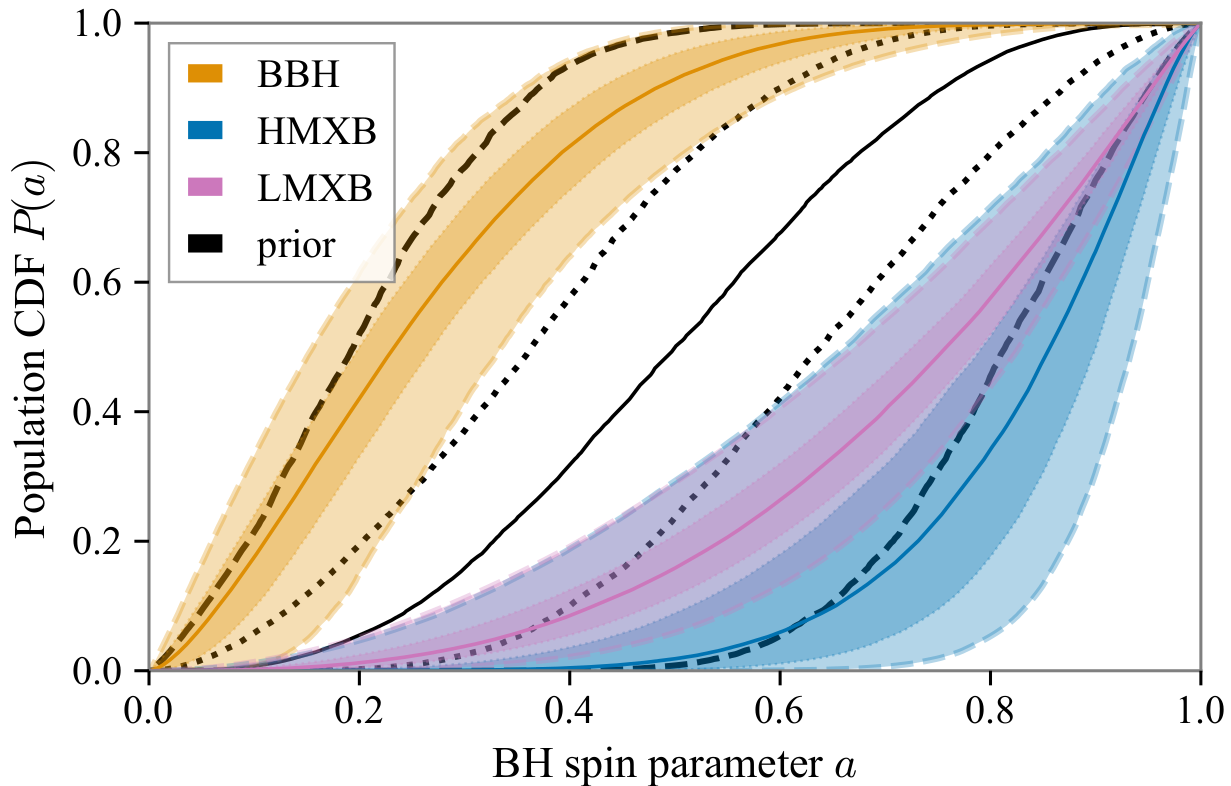
\includegraphics[width=\textwidth]{./images/tensionspin.png}
	\end{minipage}
	\hfill
	\begin{minipage}{.49\textwidth}
		\vspace{.5mm}
		\centering
		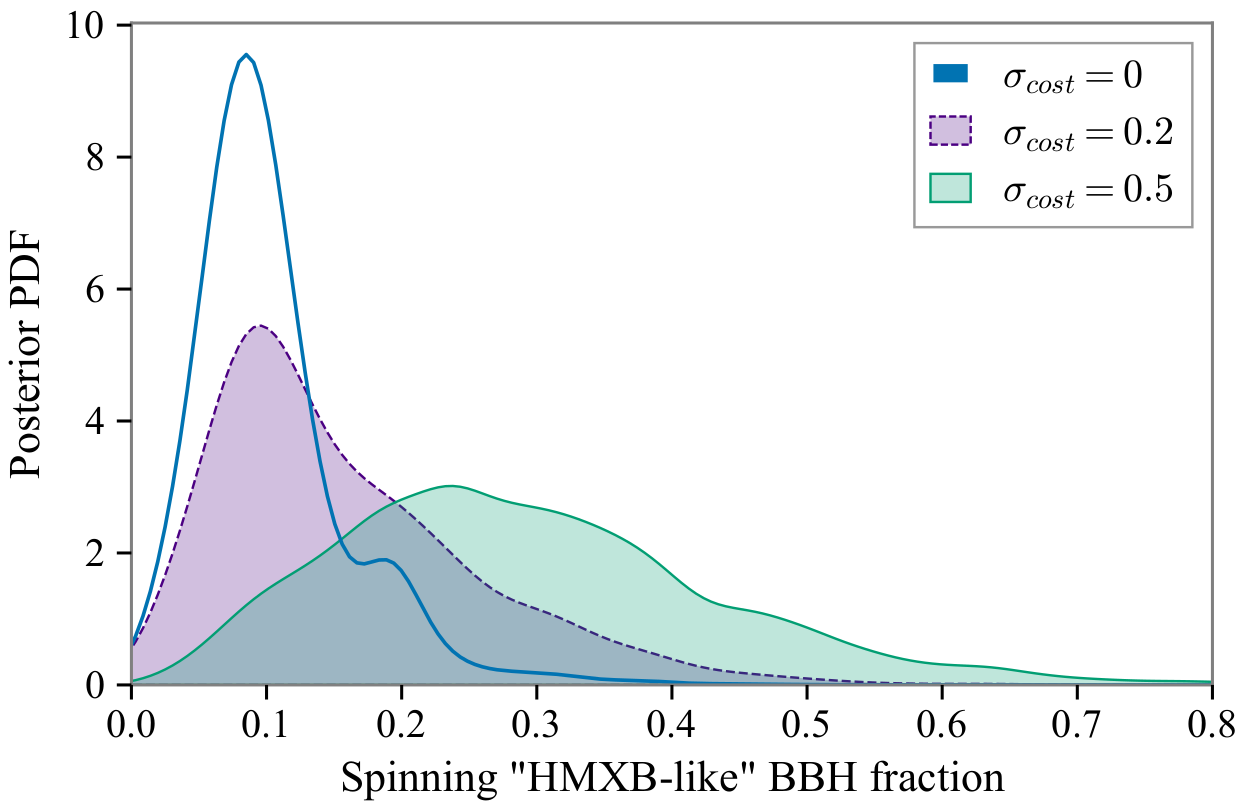
\includegraphics[width=\textwidth]{./images/tensionspinHMXBHlike.png}	
	\end{minipage}
	\caption{\emph{Left:} cumulative distribution function (CDF) of primary and secondary black hole spins detected with gravitational wave detectors in GWTC-2 (orange) compared with the ones of LMXBs (pink) and HMXBs (blue). The black lines show the prior beta distribution used for the fits. The spin distribution of the binary black holes is in tension with the ones inferred from the X-ray binaries. \emph{Right:} Posterior distributions of the fraction of binary black holes that could have evolved from a HMXB-like configuration. The more the primary spin is aligned to the orbital angular momentum (smaller $\sigma_{\rm \cos \theta}$ values, see Sec.\ \ref{subsec:tensionspin} for more detail) and the more the HMXB configuration is irrelevant in the underlying population \cite{HMXBH_spins2021}.}\label{fig:tensionspin}
\end{figure}


\subsection{Strong tension in the spin distribution}\label{subsec:tensionspin}
The spin distribution of the black holes detected with the gravitational waves (including both primary and secondary black holes) seems to be in tension with the spin distribution of the black holes detected in X-ray binaries, as visible in the left-hand panel of Fig.\ \ref{fig:tensionspin}. The LVC binary black holes appear to host slowly spinning black holes, whereas both the LMXBs and HMXBs contain fast rotating black holes. Beta distribution fits to the observed spins of the LMXBs (pink) and HMXBs (blue) denote that the two types of X-ray binaries have spin distributions consistent within 90~\%. A single beta distribution fitted to the LMXBs and HMXBs altogether exhibits a disagreement at the 99.9~\% level with the spin distribution of the LVC binary black holes (orange).\cite{HMXBH_spins2021}\\

The three HMXBs considered here (LMC X-1, M33 X-7 and Cyg X-1) host very fast spinning black holes $\chi \gtrsim 0.8$: if they produce a binary black hole in the isolated binary evolution scenario, it is likely that mass transfer and tidal locking will align the spins to the orbital angular momentum of the binary \cite{Kalogera2000_spinaligned}. Nevertheless, supernova kicks may still cause a tilt in the spin orientation. Overall, the toy model usually adopted for the tilt angles $\theta$ is a half-Gaussian in $\cos \theta$, peaked at aligned spins $\cos \theta = 1$  with some standard deviation $\sigma_{\rm \cos \theta}$: the larger the tilt angle, the larger the standard deviation \cite{spintiltmodel_Talbot2017}. % so che è un toy model ma devo comunque introdurlo perché è il toy model usato da fishbach e kalogera, i cui parametri compaiono nei grafici che mostro

It is possible that a sub-population of binary black holes has evolved through a HMXB-like configuration; Bayesian inference methods can be used to put upper limits to the fraction of binary black holes belonging to it. One of the input parameters of the inference method is the effective spin $\chi_{eff}$ i.\ e.\ the mass-weighted component of the spins aligned to the orbital angular momentum (see Eq.\ \ref{eq:chieff}). Determining the upper limits in the sub-population weight means assuming that the $\chi_{eff}$ is mainly determined by the spin of the primary black hole. Therefore, a black hole binary coming from a HMXB-like configuration will be modeled with secondary spin narrowly peak around zero and primary spin distributed with the half-Gaussian in $\cos \theta$. 

The right-hand panel in Fig.\ \ref{fig:tensionspin} shows the results of three possible estimates of the sub-population weight allowing for three different maximum tilts of the primary spin: no tilt ($\sigma_{\rm \cos \theta} = 0$), $\lesssim 12^{\circ}$ tilt ($\sigma_{\rm \cos \theta} = 0.2$) or $\lesssim 30^{\circ}$ tilt ($\sigma_{\rm \cos \theta} = 0.5$). The more the primary spin is forced to be aligned, the less the HMXB configuration is relevant in the formation history of the binary black hole. The fraction of binaries belonging to the sub-population of HMXB-like binaries is only $< 19 \% $ for aligned spins, growing to $< 30 \%$ for slightly tilted spins ($\sigma_{\rm \cos \theta} = 0.2$) and up to $< 48 \%$ for mildly tilted spins ($\sigma_{\rm \cos \theta} = 0.5$).\\

The evolutionary mechanisms necessary to create a rapidly spinning primary in a system that forms a binary black hole merging within a Hubble time are still under investigations. One of the proposed channels involves a stable mass transfer event from a main sequence donor to a main sequence accretor. If the angular momentum transport is inefficient inside the star and the mass transfer can remove its envelope tidally-locking the system, a lot of the angular momentum can be maintained in the core of the donor star. After a similar mass transfer, the donor will rapidly become a Wolf-Rayet star and eventually produce a fast spinning black hole \cite{spinfastBH_Qin2019}. Population synthesis studies coupled with detailed stellar evolution models showed that only $\lesssim 12 \%$ of the HMXB binaries formed in this way had the right combination of parameters to evolve into a black hole binary that merges via gravitational wave emission within a Hubble time. Overall, only $\lesssim 20 \%$ of the merging binary black holes seem to undergo this kind of evolution, in agreement with the upper limit of $\lesssim 30 \%$ found for slightly tilted spins \cite{HMXBHspins2022}.




%%%%%%%%%%%%%%%%%%%%%%%%%%%
%%%%%% Chapter 2 %%%%%%%%%%
%%%%%%%%%%%%%%%%%%%%%%%%%%%
\chapter{Wolf-Rayet -- black hole binaries}\label{ch:WR--BH}
\paragraph{An intermediate evolutionary stage}
The systems composed of two massive stars are the best possible progenitors for the LVC binary black holes, if the stars are massive enough to form a black hole ($\mzams \gtrsim 15-25~\msun$ at solar metallicity, according to single stellar evolution \cite{Limongi2017_handbookSN}) and if their orbit is tight enough to undergo at least one mass transfer episode: 82 O-type stars with mass $\sim 15-60~\msun$ observed in six Galactic open clusters revealed that $70 \%$ of the massive stars are born in binaries, close enough to allow for mass transfer interaction \cite{Sana2012}. 

Population-synthesis studies suggest that at least one mass transfer episode is necessary to shrink the orbit of the progenitor binary star and allow the coalescence of the two final black holes within a Hubble time \cite{spera2019_mergingBBH}. While it is difficult to predict the type of mass transfer and the fate of the binary, because they strongly depend on the orbital separation and stellar evolution details as shown in Fig.\ \ref{fig:Sana2012MTfate}, it is likely that mass transfer and strong stellar winds will strip the hydrogen envelope of a massive star and produce a Wolf-Rayet one. Therefore, if the right conditions are met, a binary evolves into a black hole -- Wolf-Rayet system and could become visible as an X-ray binary, since the strong winds of the Wolf-Rayet star can power the black hole accretion disk formation and emission.

\paragraph{Chapter outline}
This chapter reviews the theory of single stellar evolution and the main mass transfer processes (wind-fed accretion, Roche lobe overflow, and common envelope) to better understand the evolution of Wolf-Rayet -- black hole binaries. I will report the observed properties of the known Wolf-Rayet -- black hole systems, discussing the main issues in parameter estimation. Finally, I will describe the Cyg X-3 system: the only known Galactic Wolf-Rayet -- black hole binary.


\begin{figure}[h!]
	\centering
	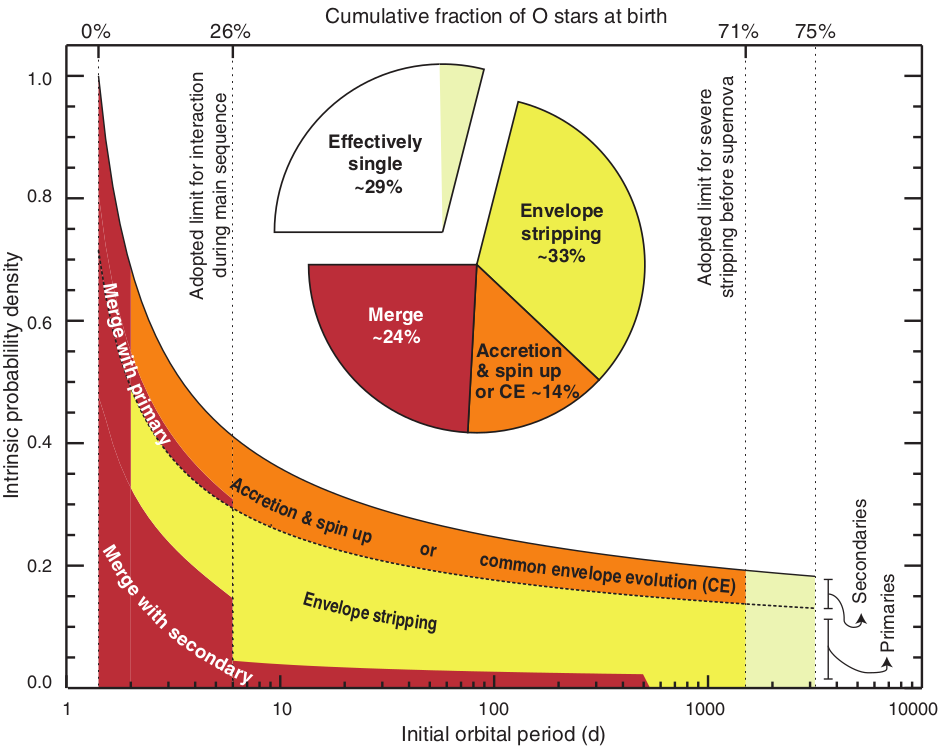
\includegraphics[width=.65\textwidth]{./images/Sana2012MTfate.png}
	\caption{70\% of O-type stars will be part of a binary with initial period $< 1500$ days and will undergo at least one mass transfer process. The type of mass transfer and the fate of the binary will depend on the details of single stellar evolution and on the orbital separation \cite{Sana2012}.}\label{fig:Sana2012MTfate}
\end{figure}



\section{Wolf - Rayet stars}
\subsection{Spectral classification of a Wolf-Rayet star}\label{subsec:WRclassification}
\paragraph{Peculiar properties} Wolf-Rayet (WR) stars are named after the French astronomers Charles Wolf and Georges Rayet that in 1867 first discovered three stars in the Cygnus constellation with strong and broad emission lines. More than a century after, a few hundreds of Wolf-Rayet stars were discovered in the Milky Way, $\sim 40 \%$ of which are part of binary systems.

Stellar spectra usually exhibit a continuum with narrow absorption lines. Generally, the hot radiation coming from the interior is absorbed by atoms and molecules in a cooler stellar photosphere ($T_{\rm eff} \lesssim 60$ kK in the hotter O-type stars). In contrast, the photosphere of Wolf-Rayet stars is much hotter ($T_{\rm eff} \sim 60 - 100$ kK) and hosts many heavy elements, often ionized (like He, N, C or O). The atoms and ions in the photosphere strongly interact with the energetic photons coming from the interior: they produce recombination and fluorescence emission lines (visible in the UV, optical and near-IR bands) while efficiently absorbing the momentum of photons via multiple-scatterings. The net effect is the production of a very dense and strong wind ($\mdot \sim 10^{-4}-10^{-5}~\msun~\yr^{-1}$) with broad emission lines of elements and ions usually absent in other stellar spectra.

\paragraph{Classification and evolutionary sequence}The spectrum of Wolf-Rayet stars is their distinctive feature and is used to classify them on the basis of the presence and abundance of peculiar elements in the photosphere. The most important lines adopted for the classification are reported in Tab.\ \ref{tab:WRclassification} and characterize the three sub-types: WN (strong lines of helium and nitrogen), WC (strong lines of helium, carbon and less prominent lines of oxygen) and WO (strong lines of oxygen and less prominent lines of helium and carbon). The WN stars can be further divided into two subfamilies on the basis of their surface hydrogen abundance $X_H$: WNL (late) if $X_H \gtrsim 0.5$ or WNE (early) if $X_H \lesssim 0.5$. In contrast, WC and WO stars lack hydrogen lines: it is probable that they lost the external envelope because of stellar winds or as a result of mass transfer.  

The helium, nitrogen, carbon and oxygen detected in the photosphere were produced by the CNO cycle and triple-$\alpha$ reactions of H- and He-burning, respectively. Usually these elements can reach the photosphere only as a result of dredge-up events, but their abundance is lower than the one detected in Wolf-Rayet stars. Recalling that the hydrogen envelope is either small or depleted, it is likely that the observed types of Wolf-Rayet stars are part of an evolutionary sequence of massive stars: the external layers are progressively removed and expose the more metal-rich ones. According to this interpretation, the evolution would proceed as

\[\rm WNL \rightarrow WNE \rightarrow WC \rightarrow WO\]

\paragraph{Type II and Ib/c supernovae} Wolf-Rayet stars that explode with little (WN) or no hydrogen envelopes (WC,WO) are likely the progenitors of, respectively, the Type II and Type Ib/Ic core-collapse supernovae. The stronger hints come from the observations of supernova light curves: Type II supernovae exhibit hydrogen lines, Type Ib lack hydrogen but exhibit He and Type Ic lack both hydrogen and helium \cite{WR_signature,parsec2015_chen,Limongi2010_preSNevo}.


\renewcommand{\arraystretch}{1.5}
\begin{figure}[h]
	\centering
		\begin{tabular}{lll}
			\toprule
			WR type & Elements & Wavelength $\lambda$ of the strongest lines \\
			\midrule
			\multirow{2}{*}{WN}  & He I-II  & 2.058 $\mu\rm m$~[He I] \\
			& N III-V & 1640 \AA , 4686 \AA, 5412 \AA, 1.012 $\mu\rm m$, 2.189 $\mu\rm m$~[He II]  \\ 
			\hline
			\multirow{2}{*}{WC}  & C III-IV  & 4650 \AA, 5696 \AA ~[C III] \\
			& O III-V & 1550 \AA,  5548-51 \AA, 5801-12 \AA, 2.08 $\mu\rm m$~[C IV] \\
			\hline
			\multirow{2}{*}{WO}  & C IV  & 3811-34 \AA~[O VI]\\
			& O V-VI & \\
			\bottomrule 	
		\end{tabular}
		\captionof{table}{Main UV, optical and near-IR emission lines used for the spectral classification of Wolf-Rayet stars \cite{WR_signature, CygX-3_Koljonen2017}} \label{tab:WRclassification}
\end{figure}



\subsection{Mass determination of a Wolf-Rayet star}\label{subsec:massWR}
\paragraph{Dynamical masses} The mass of the Wolf-Rayet stars that are member of a binary system with a non-degenerate companion can be determined with the dynamical method described in Sec.\ \ref{subsec:Xraymeasure}. The largest uncertainties come from binary inclination, thus, observations in eclipsing binaries (for which the nearly edge-on orientation better constraints the inclination) allow the most precise mass determinations. Dynamical measurements revealed that WC stars are lighter than the WN ones, supporting the evolutionary sequence of Wolf-Rayet stars described in Sec. \ref{subsec:WRclassification}: WC are limited to $\rm M_{\rm WC}\sim 9-16~\msun$ while WN extend to $\rm M_{\rm WN}\sim 10-83~\msun$ \cite{WR_signature}.

\paragraph{Isolated Wolf-Rayet stars and Wolf-Rayet stars with a degenerate companion} The dynamical method cannot be used for stars with a degenerate companion (like a neutron star or a black hole) or for the isolated ones. Furthermore, the dense stellar wind of Wolf-Rayet stars prohibits reliable measurements of the surface gravity from the photospheric lines. 

The only method left relies on the theory of stellar evolution.  Detailed calculations can relate the mass of a star in a given evolutionary stage to its expected observable properties, including its luminosity. If the distance and age of the Wolf-Rayet star are known (for instance for  Wolf-Rayet stars in star clusters), it is possible to reconstruct its intrinsic luminosity. Thus, to determine the mass of an isolated Wolf-Rayet star it is sufficient to measure its luminosity and adopt a mass-luminosity relation obtained from theoretical calculations. It is important to note that the mass-luminosity relations strongly depend on stellar evolution assumptions and need to be carefully calibrated, for instance with Wolf-Rayet stars in binary systems whose mass is already known from dynamics \cite{Nugis2000_WRwinds}.

\paragraph{Upper mass-luminosity relation} The luminosity of a star depends on the nuclear reactions acting in the core of the star and, thus, on the chemical composition. In general, stars that are not chemically-homogeneous and have a mean molecular weight higher in the core and lighter in the surface. However, considering a homogeneous star allows to put an upper limit on the mass related to a given luminosity: if the core is lighter (because of the chemical homogeneity imposed) more mass is required to produce the same luminosity. 

The left-hand panel of Fig.\ \ref{fig:MLandwinds} shows the quadratic dependence of the luminosity on the mass of chemically-homogeneous stars. The same massive star is more luminous if the core is heavier, with a linear dependence of the luminosity on the hydrogen abundance $X_H$: the less the hydrogen content in the large convective core, the higher the mean molecular weight, thus, the higher the surface luminosity \cite{Grafener2011_M-L_WR}.
 
 
\begin{figure}[h]
	\begin{minipage}{.49\textwidth}
		\centering
		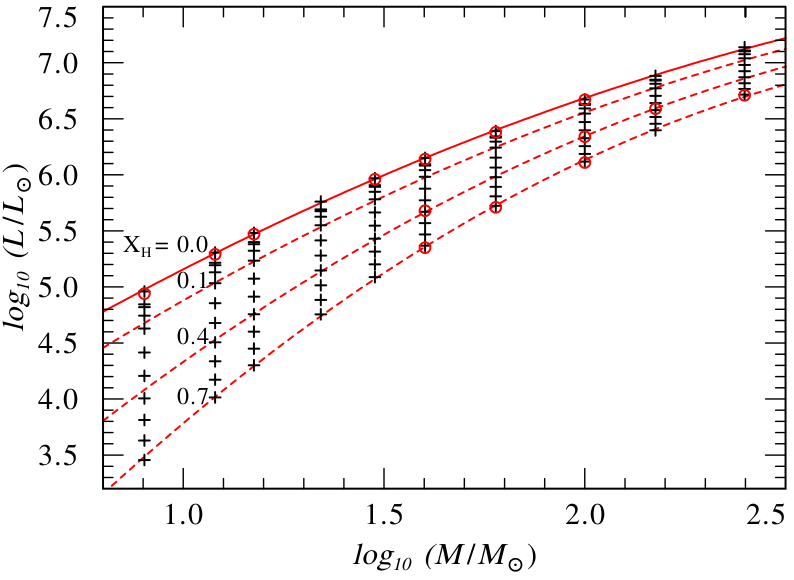
\includegraphics[width=.94\textwidth]{./images/MLrelation.png}
	\end{minipage}
	\hfill
	\begin{minipage}{.49\textwidth}
		\centering
		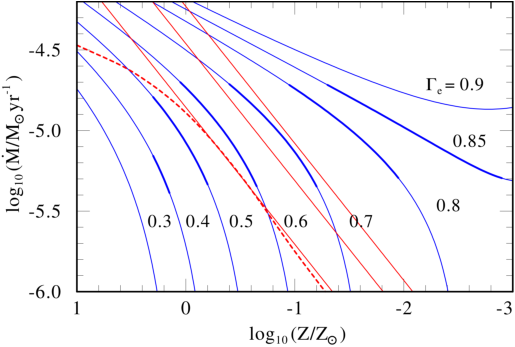
\includegraphics[width=\textwidth]{./images/stellarwinds.pdf}	
	\end{minipage}
	\caption{\emph{Left:} Mass-luminosity relations for chemically-homogeneous massive stars with fixed hydrogen abundance $X_H$. The black crosses indicate the computed stellar models, the dashed red lines the fits for hydrogen-core burning stars with different $X_H$, the solid red line indicates pure-He stars ($X_H = 0$) burning helium in their cores \cite{Grafener2011_M-L_WR}. \emph{Right:} Mass loss rates dependent only on the metallicity as in Vink et al.\ \cite{Vink2001} (red solid lines) or also on the Eddington factor as in Gr{\"a}fener \& Hamann \cite{G&H_WRmassloss} (blue solid lines). The simplified model of Vink et al.\ strongly underestimates the mass lost by low-metallicity stars close to the Eddington limit $\Gamma_e \sim 1$. The red dashed line indicates a model not considered in this thesis \cite{G&H_WRmassloss}.}\label{fig:MLandwinds}
\end{figure}

\subsection{Stellar winds of massive stars}\label{subsec:stellarwinds}
\paragraph{Metallicity dependence} O, B and Wolf-Rayet stars are massive and hot stars with $\rm T_{\rm eff} \gtrsim 12$~kK that emit the bulk of photons in the UV regime and suffer \emph{line-driven winds}. The radiation coming from the star interior is so energetic that ionizes metals\footnote{In astronomy, metals indicate elements heavier than He and their total mass fraction is expressed as metallicity $Z$.} like C, N, O, Ne, Si, S and Fe in the photosphere. Ions absorb the momentum of the impinging photons and are accelerated. However, moving in a plasma, ions share their momentum with nearby nuclei and electrons and undergo multiple scatterings, with the net effect of accelerating the whole gas. Intuitively, higher temperatures and metal content favour the production of ions, increasing the amount of momentum absorbed and, eventually, the mass loss.\\

In 2001, Vink et. al.\ \cite{Vink2001} carried out Monte Carlo simulations on a grid of 540 models of O and B main-sequence stars, quantifying the dependence of the mass loss rate $\mdot$ on the metallicity $Z$ and effective temperature $\rm T_{\rm eff}$ as

\begin{equation}\label{eq:Vink2001}
\dot{M} \propto Z^{0.85}~v_\infty^p \quad \quad p = 
\begin{cases}
-1.23 & T_\textup{eff} \gtrsim \SI{25}{kK} \\
-1.60 & \SI{12}{kK} \lesssim T_\textup{eff} \lesssim \SI{25}{kK}
\end{cases}
\end{equation}

where $v_\infty$ is the terminal velocity of the wind, reached when the gas is far enough from the star that is no more accelerated by the radiation field. The mass loss rate depends also on the stellar mass and luminosity; although with slightly different exponents for the different temperature ranges, the order-of-magnitude dependence is $\mdot \propto L^{2.2} M^{-1.3}$. \\

In 2000, Nugis \& Lamers \cite{Nugis2000_WRwinds} observed 34 WN and 30 WC stars in the Milky Way and expressed the mass-loss rate for Wolf-Rayet stars as a function of metal ($Z$) and He ($Y$) mass fractions

\begin{equation}\label{eq:NugisLamers2000}
	\mdot \sim 1.0 \times 10^{-11}~(L/L_\odot)^{1.29}~Y^{1.7}~Z^{0.5}~\msun~\yr^{-1}
\end{equation}


In 2005, Vink \& de Koter \cite{VinkDeKoter2005_stellarwindsFe} carried out further Monte Carlo simulations and demonstrated that line-driven winds in O, B and Wolf-Rayet stars are, instead, strongly sensible to multiple absorption and re-emission of Fe lines and, in metal poor environments, also of C, N and O lines. Following this result, Costa et al.\ \cite{MassGapStellarEvo_Costa2021} developed an updated prescription for Wolf-Rayet stellar winds. They adopted revised mass-loss fits extracted by Sander et al.\ \cite{Sander2019_WRwinds} from observations on Galactic WC and WO stars and accounted for the dependence on the iron mass fraction $X_{\rm Fe}$ by adding two multiplicative factors for WN and WC stars, calibrated on fits to WN and WC models calculated in 2015 by Vink et al.\ \cite{Vink2015_stellarwindsFe}

\begin{equation}\label{eq:Costa2021Sander2019}
    \mdot = f_{\rm WR}~ 10^{-8} ~ (L/L_\odot)^{0.68} ~\msun~\yr^{-1} \quad \quad f_{\rm WR} = 
\begin{cases}
-1 + 1.9 \tanh{[0.58 (\log X_{\rm Fe} +1)]} & \text{WN} \\
-0.3 + 1.2 \tanh{[0.5 (\log X_{\rm Fe} +0.5)]} & \text{WC}
\end{cases}
\end{equation}

In fact, in 2022 Sander et al.\ \cite{Sander2022_WRwindsupdate} adopted a self-consistent description for the atmosphere of WN stars and derived theoretical mass-loss rates less efficient than the ones found by Nugis \& Lamers. Sander et al.\ argued that C and O are not so much relevant to power Wolf-Rayet stellar winds as Nugis \& Lamers assumed: including, as Nugis \& Lamers did, C and O abundance in the metallicity-term causes unrealistically high mass-loss rates. Moreover, comparing stellar evolution models evolved with \texttt{MESA} with different stellar winds prescriptions, Sander et al.\ noted that metal-rich Wolf-Rayet stars (down to $0.1 ~\zsun$) evolved with Nugis \& Lamers winds ended almost with the same masses regardless of the metallicity.

\paragraph{Eddington factor dependence}
Hot stars like the O,B and the Wolf-Rayet have radiative external envelopes: the radiation pressure of the energetic photons produced in the core pushes on the free electrons, that interact via Thomson scattering and efficiently transport energy outwards. However, the radiation pressure can be so strong to overcome the self-gravity of the star: the external layers are no more in hydro-static equilibrium and are pushed away. The mass expelled changes the observed luminosity and the star becomes a variable; a luminous blue variable (LBV) if the original stars were of the O or B types.

Assuming that the pressure gradient of the star is due only to the Thomson scattering (with opacity $k$), the self-gravity of the star cannot support the hydro-static equilibrium if the luminosity $L$ exceeds the Eddington one $L_{\rm Edd}$. The maximum permitted luminosity $L=L_{\rm Edd}$ defines the \emph{Eddington limit} $\Gamma_e$

\begin{equation}\label{eq:Eddingtonfactor}
\Gamma_e = \frac{L}{L_\textup{Edd}} = \frac{L k}{4 \pi c G M}
\end{equation}

The Eddington factor for a fully ionized plasma is given by

\begin{equation}\label{eq:EddingtonObserved}
\Gamma_e = 10^{-4.813}~(1+X_H)~(L/L_\odot)~(M_\odot/M).
\end{equation}

The surface abundance of hydrogen $X_H$ is known from spectroscopic observations. Measuring the intrinsic luminosity and adopting the mass-luminosity relations, as described in Sec.\ \ref{subsec:massWR}, it is possible to recover the Eddington factor of the observed stars.\\


Stars that approach and overcome the Eddington limit $\Gamma_e \geq 1$ have enhanced mass loss and are likely the progenitors of the Wolf-Rayet stars, as discussed in Sec.\ \ref{subsec:stellarevo}. In fact, the evolution close to the Eddington limit, coupled with multiple scatterings in the winds, could explain the strong stellar winds of the Wolf-Rayet stars. In 2008, Gr{\"a}fener \& Hamann \cite{G&H_WRmassloss} used detailed and self-consistent modeling of non-LTE atmospheres and winds of WNL stars to compute the expected mass loss rates. A rough fit \cite{parsec2015_chen} to their relations underlines a continuity to the 2001 models of Vink et al.\

\begin{equation}\label{eq:WRwindGH2008}
\dot M \propto Z^{\alpha} \quad \quad  \alpha = 
\begin{cases}
0.85 & \Gamma_e < 2/3 \\
2.45-2.4~\Gamma_e & 2/3 \leq \Gamma_e \leq 1
\end{cases}
\end{equation}

Gr{\"a}fener \& Hamann found that the metallicity-dependence of Eq.\ \ref{eq:Vink2001} is enhanced for stars closer to the Eddington limit. As shown in the right-hand panel of Fig \ref{fig:MLandwinds}, not accounting for the dependence on $\Gamma_e$ results in a severe underestimation of the mass loss rates, especially at lower metallicities.\\

Vink et al.\ in 2011 \cite{Vink2011} re-calculated the mass loss rates on models of massive and very massive stars ($40-300~\msun$) including a dependence on the Eddington factor, finding

\begin{equation}\label{eq:Vink2011}
\begin{cases}
\dot M \propto M^{0.68}\ \Gamma_e^{2.2} & 0.4 \lesssim \Gamma_e \lesssim 0.7 \\
\dot M \propto M^{0.78}\ \Gamma_e^{4.77} & \Gamma_e \gtrsim 0.7
\end{cases}
\end{equation}


\subsection{Evolution of a massive star into a Wolf-Rayet}\label{subsec:stellarevo}

In this section I will discuss the evolution of the massive stars with particular attention to the conditions that favor the creation of Wolf-Rayet stars. I considered only stars with initial masses $\mzams \geq 20~\msun$, massive enough to likely produce a black hole in place of a neutron star after the core-collapse supernova (see Sec.\ \ref{subsec:SNmodels}), and with $\mzams \leq 100~\msun$, to avoid the discussion of the pair-instability supernovae that form at $Z=0.002$: the work of this thesis only focuses at solar metallicity $Z\sim 0.02$ where this phenomenon is not relevant \cite{spera2017_pisnSNe}. I will refer to the evolutionary tracks shown in Fig.\ \ref{fig:HRdiagrams} and \ref{fig:masslostWR} that I generated with the population-synthesis code \texttt{SEVN} \cite{spera2019_mergingBBH} interpolating the output tables of the \texttt{PARSEC} stellar evolution code \cite{parsec2015_chen,MassGapStellarEvo_Costa2021} (further details in Sec.\ \ref{sec:SEVN}). The scope of this section is to provide a self-consistent reference to the work carried out in this thesis and presented in Sec.\ \ref{sec:results}. 

\paragraph{Wolf-Rayet stars with \texttt{PARSEC} and \texttt{SEVN}} 
The \texttt{PARSEC} stellar evolution code classifies Wolf-Rayet star sub-types WNL,WNE and WC according to the surface abundance of many elements (hydrogen, helium, carbon, nitrogen, oxygen and iron) at different metallicities. For instance, at solar metallicity, the surface hydrogen fraction of WNL is $X_{\rm WNL} \leq 0.3$ while WNE and WC are consistent with no hydrogen $X_{\rm WNE} = X_{\rm WC} = 0$. In contrast, \texttt{SEVN} considers a star as a Wolf-Rayet imposing a condition \emph{only} on the \emph{total} hydrogen mass fraction, requiring that $X_H \leq 0.02$\footnote{In particular, \texttt{SEVN} computes the condition with respect to the helium mass fraction: a star in \texttt{SEVN} becomes a Wolf-Rayet if $M_{\rm He} > 97.9 \%~M_{\rm tot}$ (Iorio et al.\ in preparation).}. Stars with so little hydrogen are interpolated with different evolutionary tables, often indicated as \emph{pure-He} tables. Pure-helium tracks are computed with \texttt{PARSEC} starting from a helium zero age main sequence (He-ZAMS) i.\ e.\ a star obtained removing the hydrogen envelope to a normal star at the beginning of the core-He burning phase \cite{spera2019_mergingBBH}.\\
% le abbondanze usate come soglia da parsec non sono più quelle di Chen 2015. Qui mi riferisco alle nuove tracce generate da Guglielmo, che ha usato Hsup = XH < 0.3 a metallicità solare


The stellar winds adopted to generate with \texttt{PARSEC} the interpolating tracks for massive stars account for the dependence on  both metallicity and the Eddington factor (see Sec.\ \ref{subsec:stellarwinds} for more details). While mass loss rates of the blue super giants (BSG) and LBVs follow Vink et al.\ \cite{Vink2001} and Gr{\"a}fener \& Hamann \cite{G&H_WRmassloss} (Eq.\ \ref{eq:WRwindGH2008}), Wolf-Rayet stellar winds follow different prescriptions for different classifications: stars evolved from He-ZAMS have winds from the work of Nugis \& Lamers (Eq.\ \ref{eq:NugisLamers2000}) while Wolf-Rayet stars evolved from usual ZAMS implement the mass loss rates described by Costa et al.\ \cite{MassGapStellarEvo_Costa2021} and based on the observations of Sander et al.\ \cite{Sander2019_WRwinds} (Eq.\ \ref{eq:Costa2021Sander2019}). Even though winds of Nugis \& Lamers likely need to be revised (as discussed in Sec.\ \ref{subsec:stellarwinds}), they were adopted in pure-He stars because their mass loss rates were higher than the ones from Costa et al.\ , thus avoiding the production of Wolf-Rayet stars too light and long lived with respect to what is expected from standard stellar evolution (for instance, they produced a $2~\msun$ Wolf-Rayet star from a $8~\msun$ one, see Iorio et al.\ for more details). \\
%\micmap{In realtà no, usiamo Graefener \& Hamann anche per le WR}\erika{Ah, non era indicato sul paper di Chen 2015 da cui ho tratto tutte le informazioni su parsec... grazie dell'update}\micmap{No ho appena controllato. mi sbagliavo io: in mobse usiamo graefener ma in parsec nugis. Hmm...non sono molto contenta ma così è. ne parlo dopo con guglielmo}\erika{Riguardando il paper di Giuliano ho appena notato che dice che hanno usato Sander 2019 per i venti delle WR ma implementati secondo Costa 2021. Sono i venti usati per generare le tracce di parsec o quelli applicati da sevn? Mi sa che chiederò a Giuliano o Guglielmo lunedì in caso}\micmap{scusa...ho fatto confusione io per mancanza di memoria e perché abbiamo cambiato ormai 1000 volte. Da costa et al. 2021 in poi abbiamo cambiato da nugis a Sander (modificato per la $Z$ come scrive guglielmo in sec 2.1 del suo paper). per le tracce che poi sono finite in abbiamo cambiato mille volte perché usando sander ci siamo accorti che i venti di sander sono molto maggiori di quelli di nugis a basse masse. questo produceva delle stelle pureHe ETERNE, perché una WR di 8 msun perdeva massa fino a diventare 2 Msun e poi viveva per sempre. Allora alla fine in sevn abbiamo deciso di usare Sander per le stelle WR delle tracce H-rich ma di continuare a usare nugis per le stelle pureHe. ovviamente questo può cambiare ancora 1000 volte perché il problema è che non c'è una descrizione soddisfacente per tutte le WR. perdonami, mi ero proprio dimenticata. oggi ho rivangato tutta la discendenza (e per un certo periodo avevamo usato anche graefener, che tra l'altro viene ancora usato in mobse..)} % pluto


In this thesis I will classify a star as a Wolf-Rayet following \texttt{PARSEC}, thus requiring that its surface hydrogen is $X_H \geq 0.3$. Under this assumption, the Wolf-Rayet sample will not be limited to the pure-He stars identified by \texttt{SEVN} (representative of WC and WO sub-types) but will also include spectroscopic Wolf-Rayet stars that are still able to retain a small H-envelope (representative of WNL and WNE sub-types). Nevertheless, with this approach the minimum mass needed to produce a Wolf-Rayet star is higher with respect to other known works in the literature. In particular, the threshold found interpolating \texttt{PARSEC} tracks with \texttt{SEVN} is $\sim 5-10~\msun$ higher than the one obtained with another popular stellar evolution code, \texttt{FRANEC} \cite{Limongi2010_preSNevo}. The main differences are in the amount of core overshooting\footnote{According to the mixing-length-theory, the mean free path $l_c = \Lambda_c H_p$ of the convective bubbles that overshoot into the upper radiative envelope can be parameterize as a fraction $\Lambda_c$ of the pressure scale height $H_p$ \cite{parsec2015_chen}.} in the central H-burning phase (0.2 $H_p$ in \texttt{FRANEC} and 0.5 $H_p$ in \texttt{PARSEC}) and in the threshold to classify a star as a Wolf-Rayet ($X_H \leq 0.4$ in \texttt{FRANEC} and $X_H \leq 0.3$ in \texttt{PARSEC}). Given that Wolf-Rayet stars evolve with increased depletion of the hydrogen envelope, the $X_H \leq 0.4$ condition in \texttt{FRANEC} allows to form Wolf-Rayet stars earlier than in the \texttt{PARSEC} tracks interpolated by \texttt{SEVN}. In particular, \texttt{FRANEC} lowers the minimum initial mass required to form a Wolf-Rayet at solar metallicity to $\mzams \sim 30~\msun$, while the \texttt{PARSEC} tables interpolated by \texttt{SEVN} require a minimum mass of $\mzams \sim 40~\msun$. 




\begin{figure}[h!]
	\begin{minipage}{.49\textwidth}
		\centering
		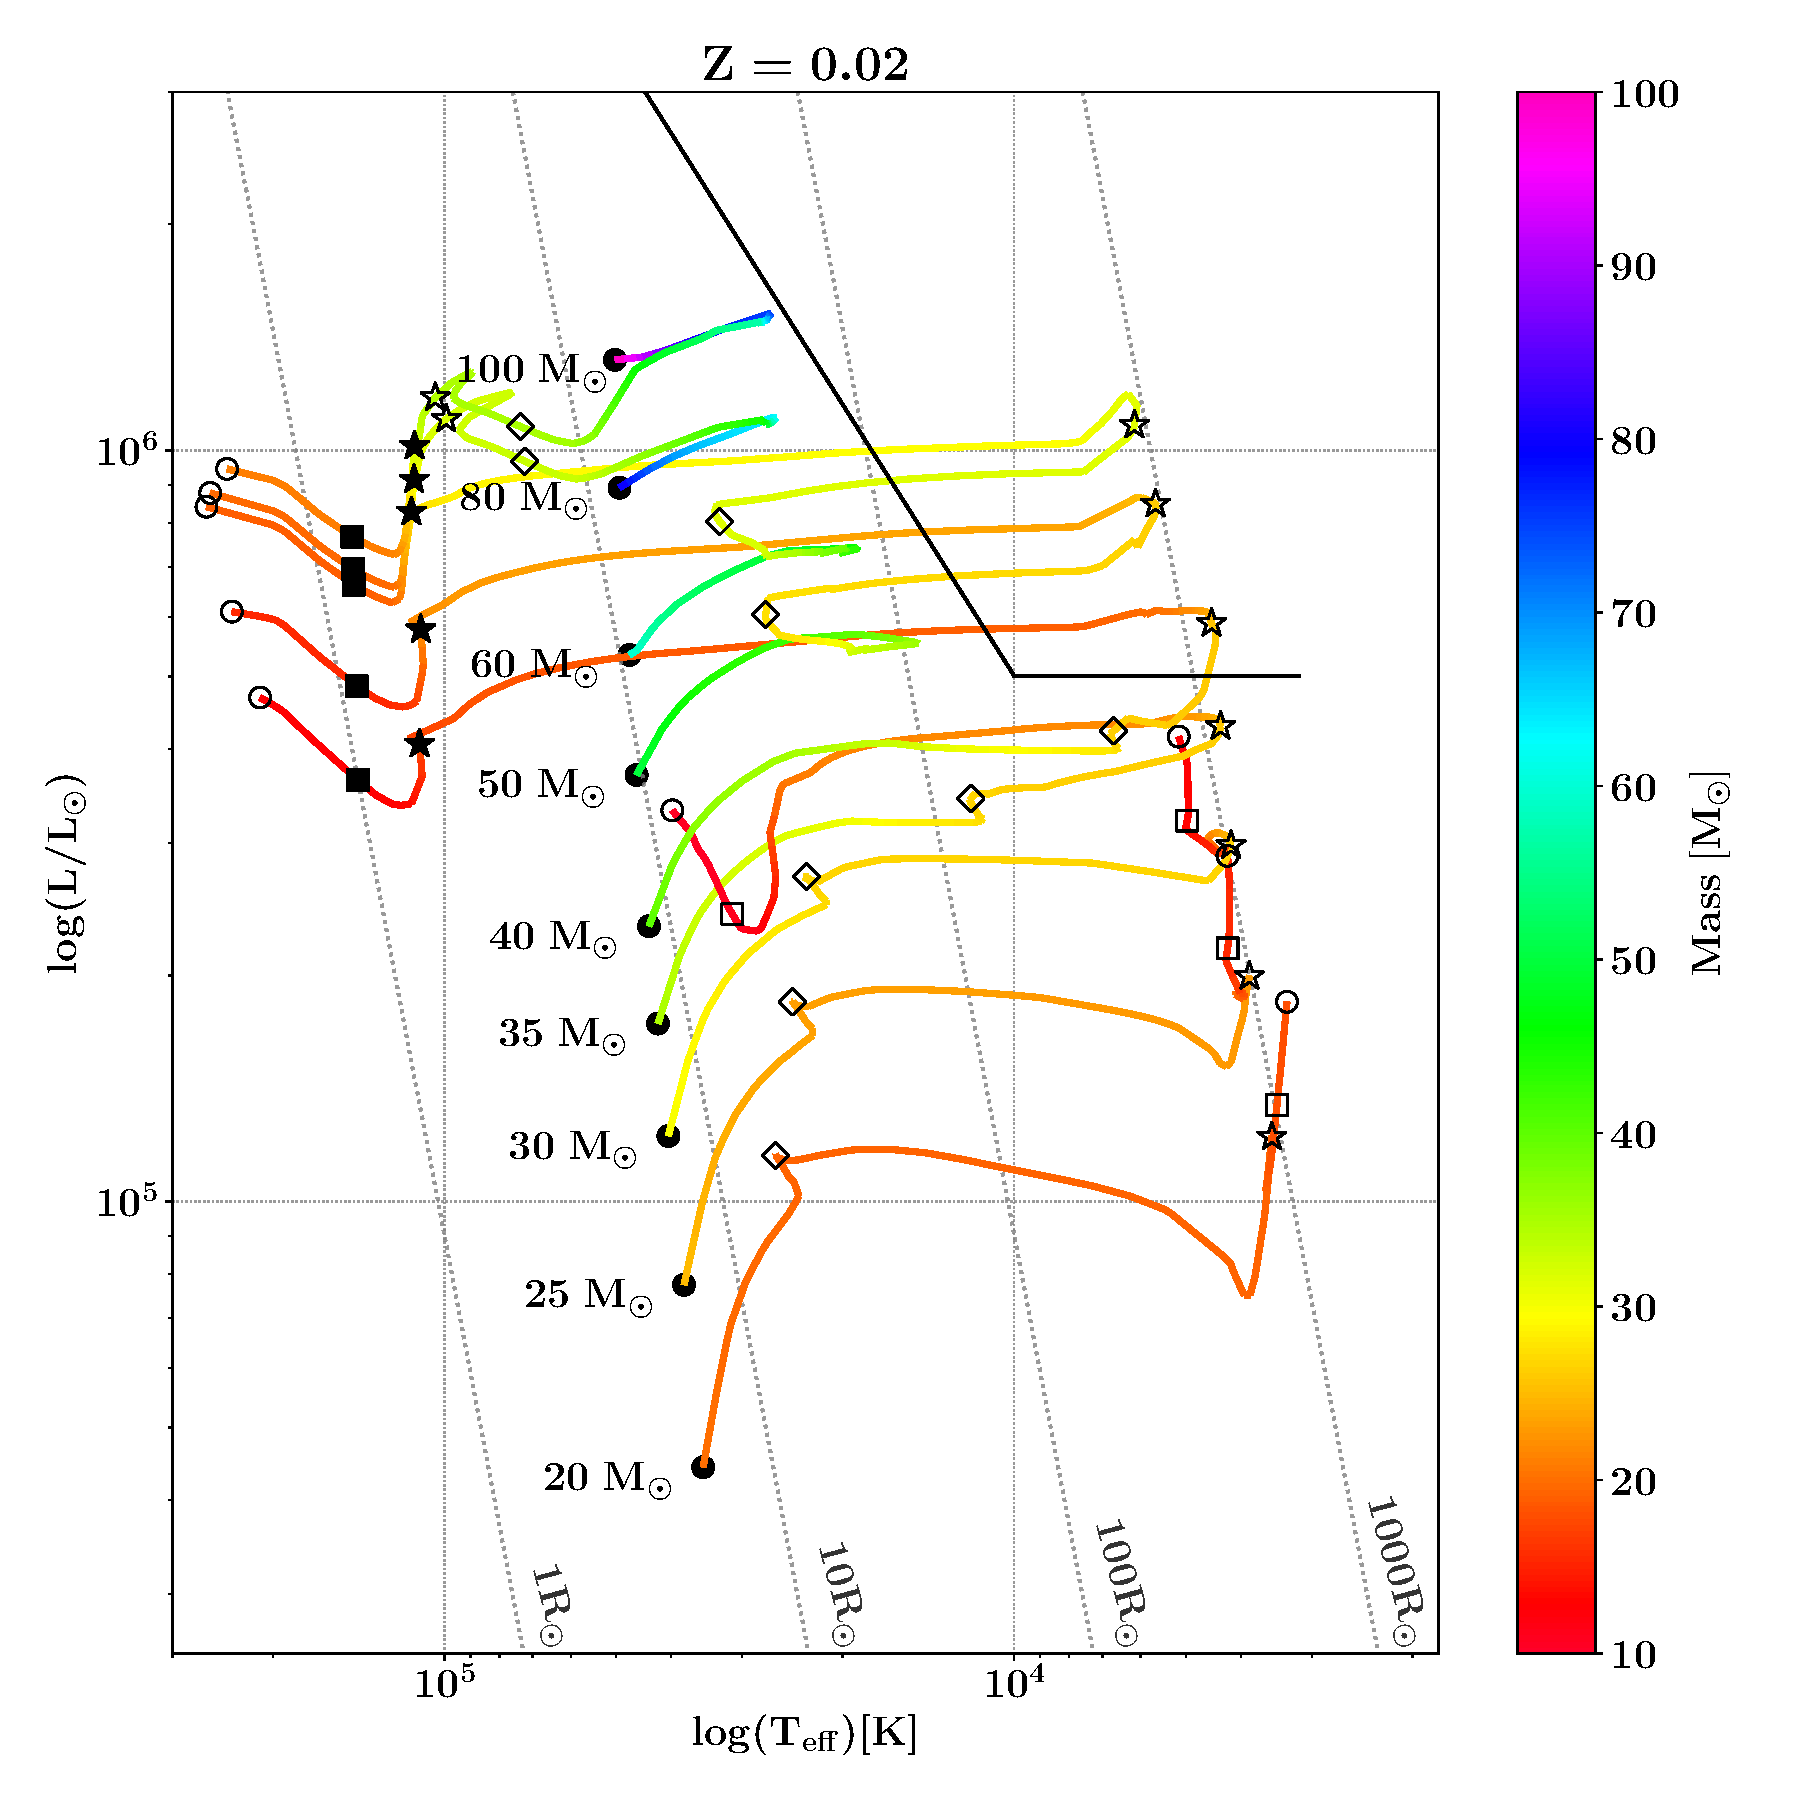
\includegraphics[width=1.05\textwidth]{./images/HR_02.pdf}
	\end{minipage}
	\hfill
	\begin{minipage}{.49\textwidth}
		\centering
		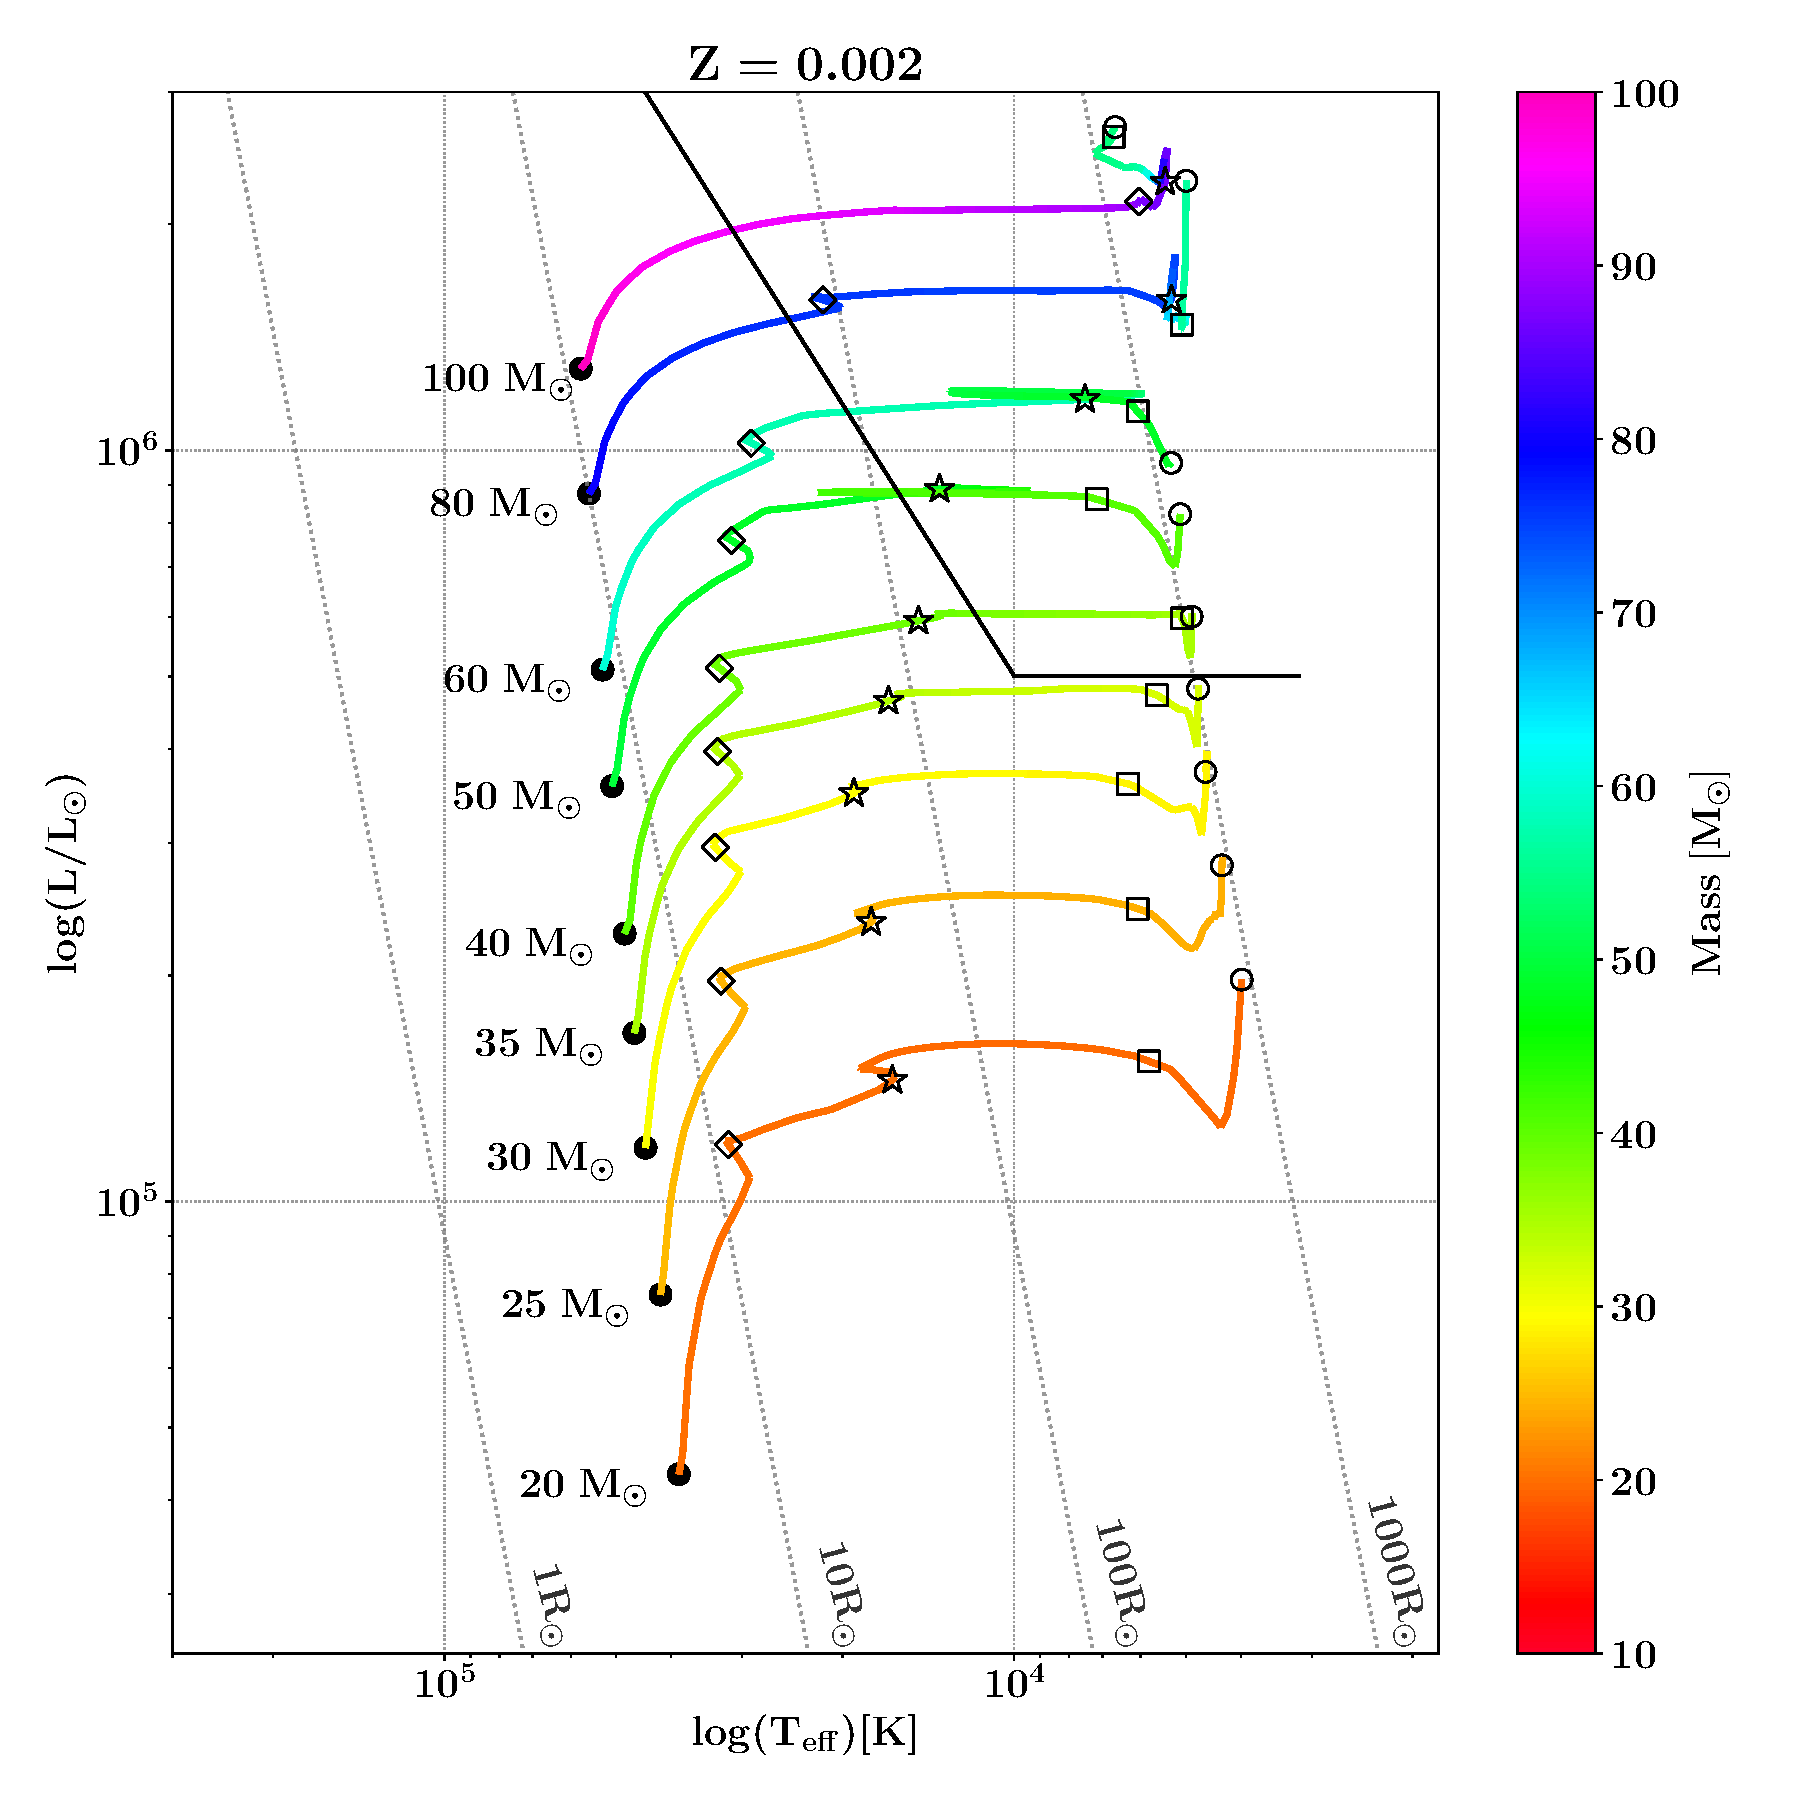
\includegraphics[width=1.05\textwidth]{./images/HR_002.pdf}	
	\end{minipage}
	\caption{Hertzsprung-Russell diagrams with the single stellar evolution of massive stars at two different metallicities. The symbols indicate the different burning stages: beginning of core H burning i.\ e.\ ZAMS (filled circle), beginning of H shell burning (empty diamond), beginning of the core He burning (empty star) possibly as a Wolf-Rayet (filled star), beginning of He shell burning (empty square) possibly as a Wolf-Rayet (filled square), end of the CO burning (empty circle). At solar metallicity ($Z=0.02$, \emph{left} panel) Wolf-Rayet stars can be produced by stars with $\mzams \gtrsim 40~\msun$ while at metallicity one order-of-magnitude lower ($Z=0.002$, \emph{right} panel) stellar winds are quenched and even stars with $\mzams \sim 100~\msun$ cannot become Wolf-Rayet stars. I generated the tracks with the population-synthesis code \texttt{SEVN} \cite{spera2019_mergingBBH}, that interpolates the tables produced with the \texttt{PARSEC} stellar evolution code \cite{parsec2015_chen} (more details on the codes in Sec.\ \ref{sec:SEVN}).}\label{fig:HRdiagrams}
\end{figure}


\begin{figure}[h!]
	\begin{minipage}{.49\textwidth}
		\centering
		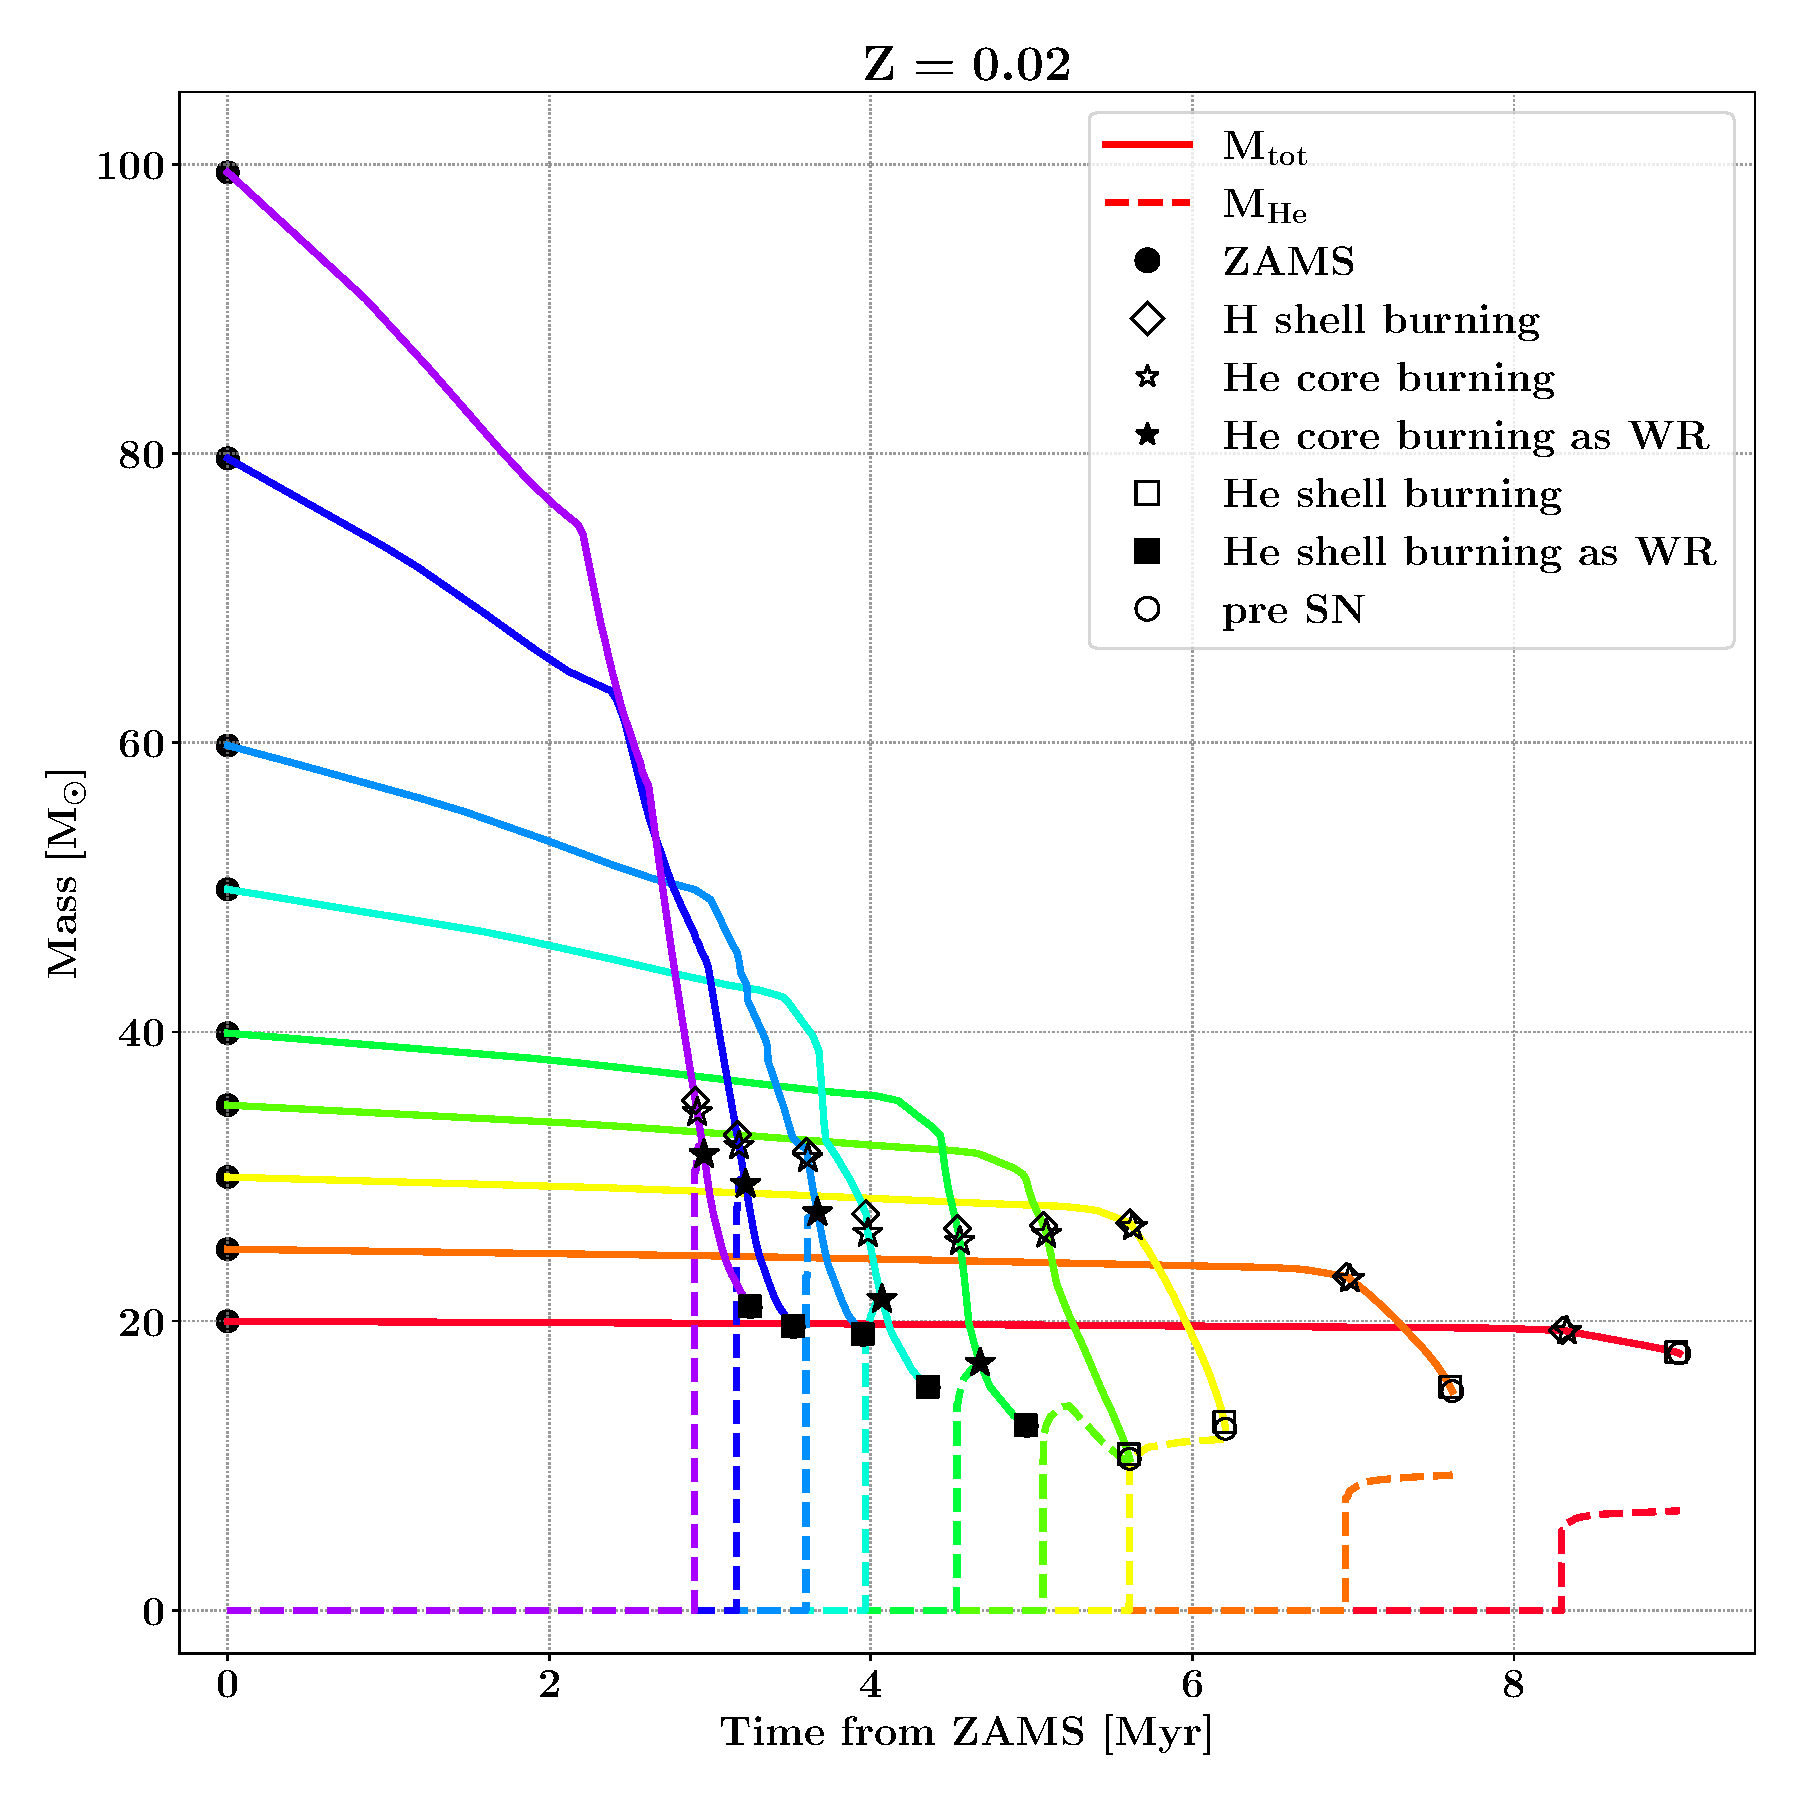
\includegraphics[width=1.05\textwidth]{./images/mass_Z02.pdf}
	\end{minipage}
	\hfill
	\begin{minipage}{.49\textwidth}
		\vspace{2mm}
		\centering
		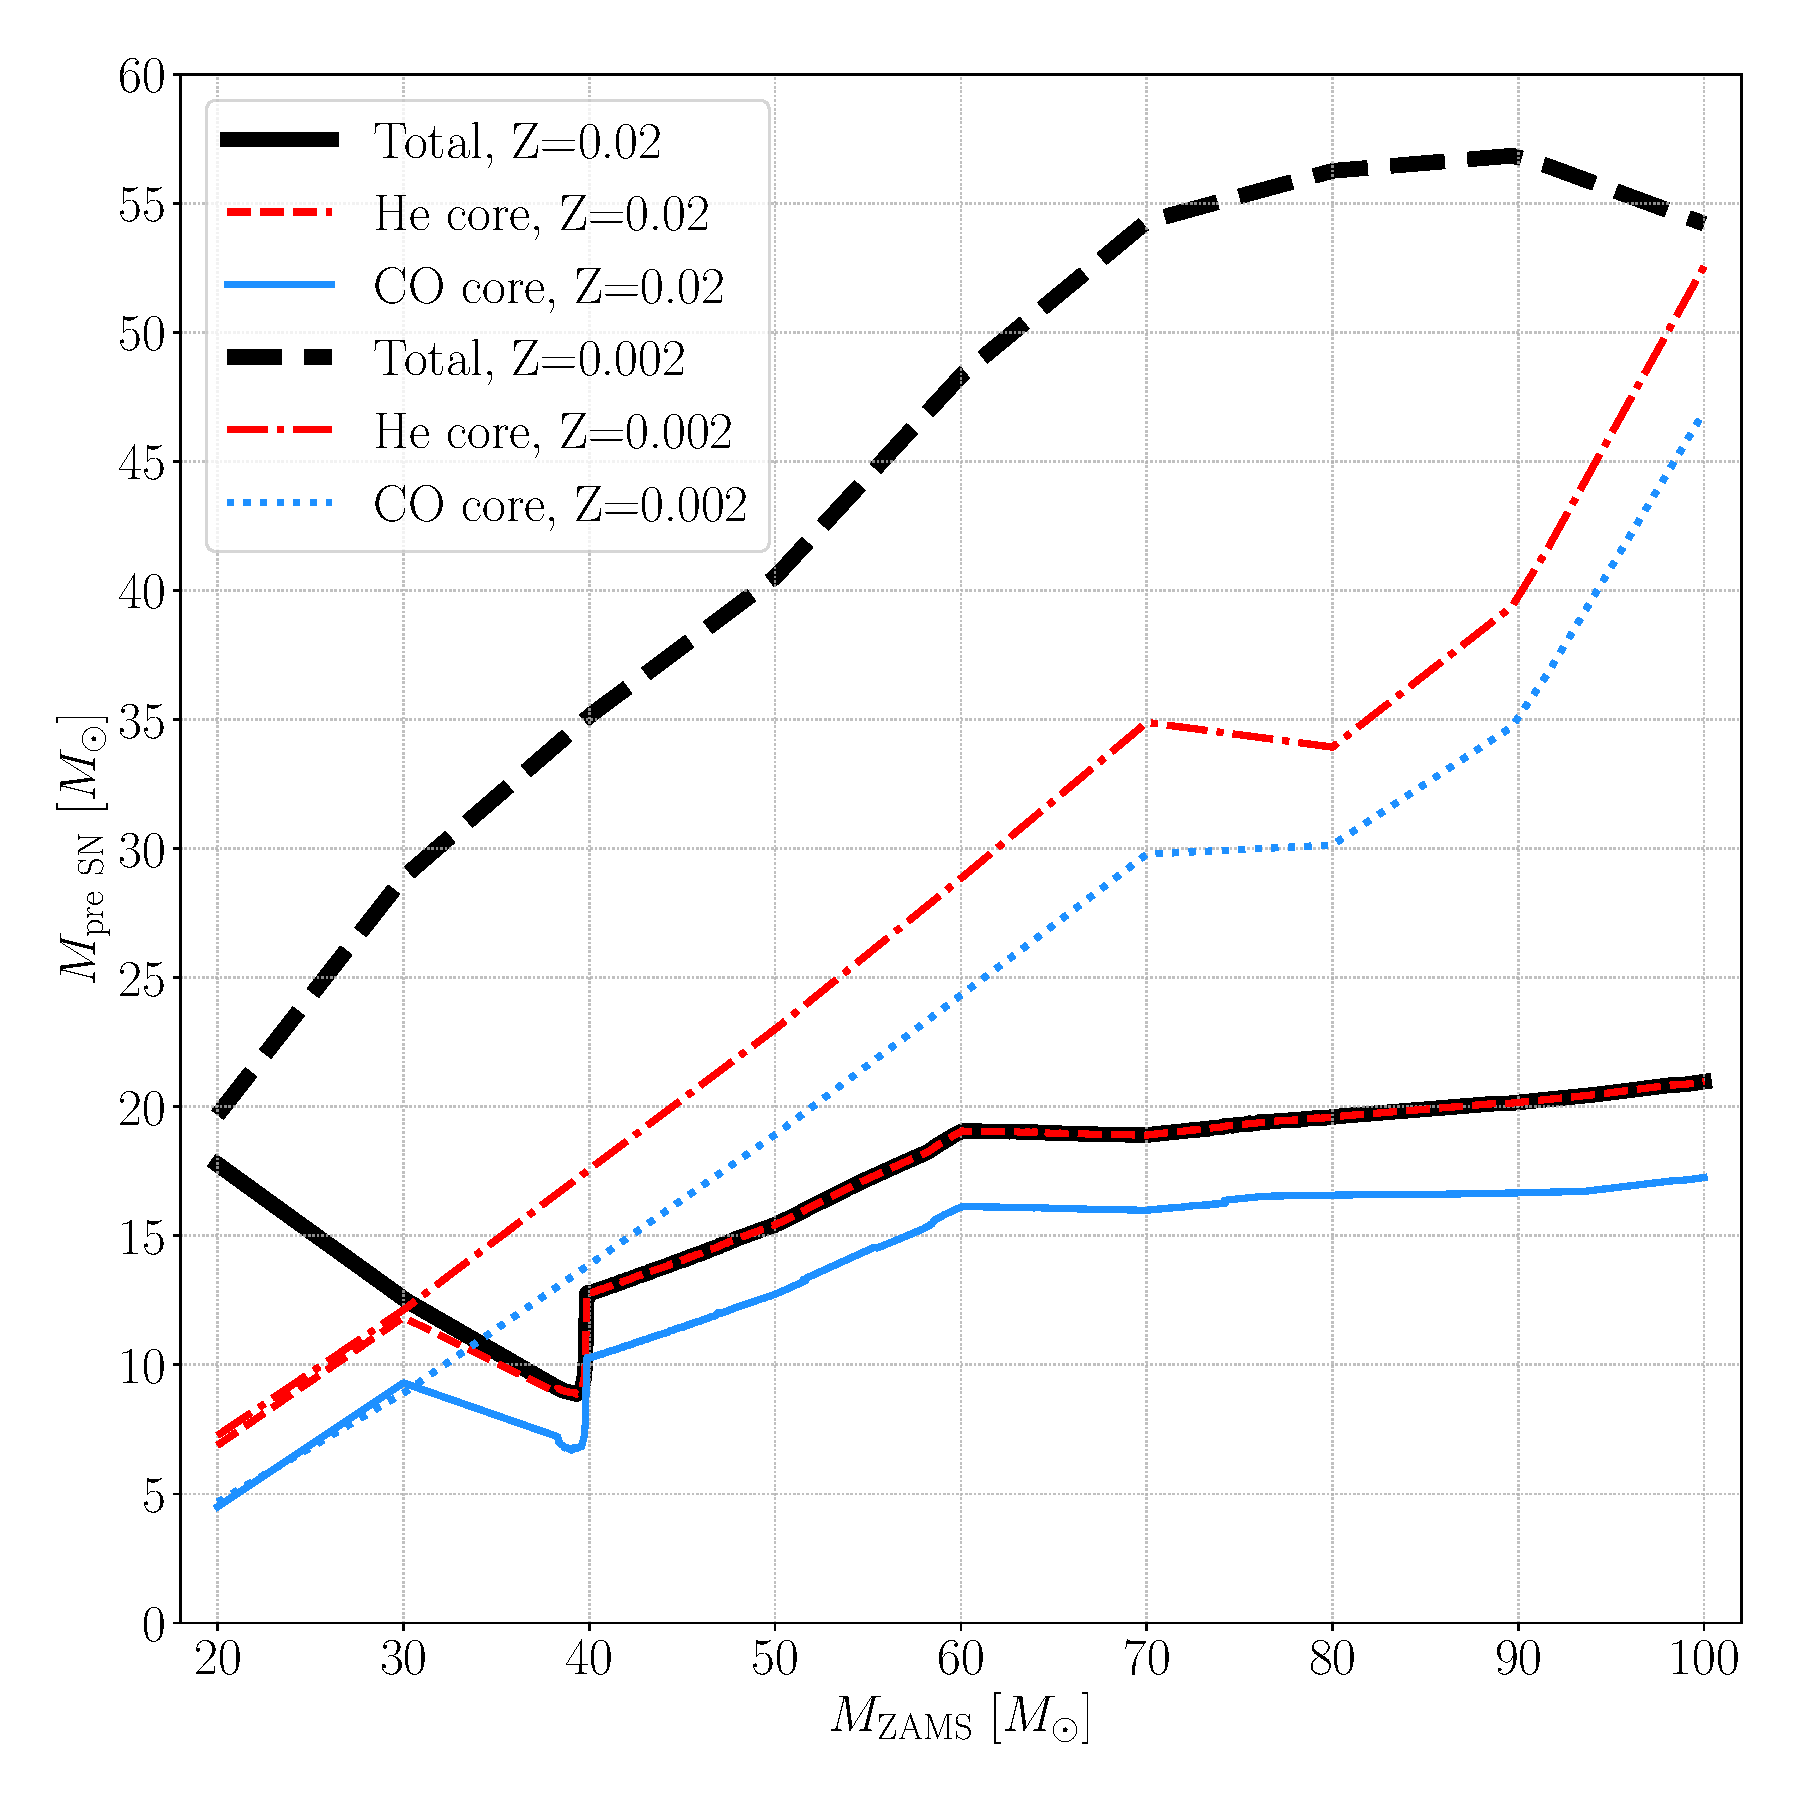
\includegraphics[width=1.05\textwidth]{./images/preSN.pdf}	
	\end{minipage}
	\caption{\emph{Left:} Time evolution of the mass of the stars (solid lines) and their He cores (dashed lines) at solar metallicity. The symbols indicate the different burning stages, as explained in Sec.\ \ref{subsec:stellarevo}. \emph{Right:} Mass of the star and of their He and CO cores at the pre-SN stage, here coincident to the end of the CO burning. At solar metallicity stellar winds strongly reduce the core sizes of stars with $\mzams \gtrsim 30 ~\msun$, transforming them into Wolf-Rayet for $\mzams \gtrsim 40 ~\msun$. At lower metallicity the cores and the stars are larger and they only reduce in stars with $\mzams \gtrsim 70-100 ~\msun$ that evolve too close to the Eddington limit. I generated both panels with the population-synthesis code \texttt{SEVN} \cite{spera2019_mergingBBH}, that interpolates the tables produced with the \texttt{PARSEC} stellar evolution code \cite{parsec2015_chen} (more details on the codes in Sec.\ \ref{sec:SEVN}).}\label{fig:masslostWR}
\end{figure}



\paragraph{Stellar evolution timescales} In this paragraph, I briefly recall the main timescales driving single stellar evolution \cite{evostellare}. The time required for a star to react to a perturbation will determine not only its evolution but, if the star is a member of a binary system, will also influence the stability and efficiency of mass transfer (further details in Sec. \ref{subsec:masstransfer}). \\

Stars are self-gravitating objects of hot plasma that remain in hydro-static equilibrium throughout their life: the internal pressure gradient of the gas and photons is balanced by the self-gravity. According to the virial theorem, perturbations of the hydrostatic equilibrium occur on the \emph{dynamical timescale}

\begin{equation}\label{eq:taudyn}
\tau_\textup{dyn} \simeq \sqrt{\frac{R^3}{G M}} \simeq 30 \left(\frac{R}{R\sun}\right)^{3/2} \left(\frac{M\sun}{M}\right)^{1/2}\ \text{minutes}
\end{equation}


The energy released by nuclear reactions is radiated from the surface and maintains the star in thermal equilibrium with $T_{\rm core} \approx const$. When the nuclear fuel is exhausted, the lower pressure gradient of the plasma causes a contraction of the star, in order to maintain the hydrostatic equilibrium. Part of the gravitational energy is radiated away but part of it heats up the interior, until it reaches the critical temperature to ignite heavier elements. The contraction is quasi-static and maintains the hydrostatic equilibrium. However, since a part of the energy produced by the contraction is not radiated away but heats up the interior, the process happens outside thermal equilibrium and occurs in a \emph{thermal timescale} (also known as \emph{Kelvin-Helmholtz timescale})

\begin{equation}\label{eq:tauth}
\tau_\textup{th} \simeq \frac{G M^2}{R L} \simeq 15 
\left(\frac{M}{M\sun}\right)^{2} \left(\frac{R\sun}{R}\right) \left(\frac{L\sun}{L}\right)\ \text{Myr}
\end{equation}

Aside from central exhaustion, local fluctuations in the core temperature or similar perturbations due to mass transfer, a star evolves in thermal equilibrium. However, the dominant evolutionary timescale is the \emph{nuclear timescale} and quantifies the time required to burn all the nuclear fuel for a given element. The longest nuclear timescale is the one for the hydrogen burning, that is the most abundant element ($\sim 70~\%$ of the stellar mass), and provides an order-of-magnitude estimate for the stellar lifetime

\begin{equation}\label{eq:taunuc}
\tau_\textup{nuc} \simeq 10 \left(\frac{M}{M\sun}\right) \left(\frac{L\sun}{L}\right)\ \text{Gyr}
\end{equation}

\paragraph{Stellar evolution from the ZAMS to the end of the CO burning} Stars begin their life in the \emph{Zero Age Main Sequence} (ZAMS, filled circles) when their cores have temperatures $T_{\rm core} \gtrsim 10^{7}$ K high enough to ignite hydrogen in the core. The evolution proceeds in the \emph{main sequence} (MS) phase until the central hydrogen is exhausted \cite{evostellare}. 

During core H-burning, stars satisfy the empirical mass-luminosity relation $L \propto M^3$. Recalling that the nuclear timescale $\tau_{\rm nuc}$ required to burn hydrogen is an approximate estimate of the stellar lifetime, the mass-luminosity relation of the MS substituted into the definition of the nuclear timescale of Eq.\ \ref{eq:taunuc} results in $\tau_{\rm nuc} \propto M^{-2}$: the more massive the star, the larger the luminosity caused by more efficient and rapid nuclear reactions, thus, the shorter the lifetime. For instance, the left-hand panel of Fig.\ \ref{fig:masslostWR} illustrates that, at solar metallicity, stars with $\mzams \sim 20~\msun$ live for $\sim 8$ Myrs, in contrast to more massive stars of $\mzams \sim 100~\msun$ that survive only for $\sim 3$ Myrs. Also, both stars have lifetimes much shorter than the Sun ($\sim{10}$ Gyr).

The stars considered here are so massive that, during the MS, they burn hydrogen in a large convective core surrounded by a radiative envelope. In the final stages of the core H-burning, the energy released diminishes and lowers the radiation pressure. To maintain the hydrostatic and thermal equilibrium, the core contracts and heats up again: the nuclear reactions increase again the luminosity produced and the surface effective temperature, thus, the star exhibits a left-ward hook in the Hertzsprung-Russell (HR) diagram (see Fig.\ \ref{fig:HRdiagrams}). \\

At the end of the core H-burning phase, the star is so contracted that the hydrogen shell surrounding the core is hot enough to ignite (empty diamonds). According to the mirror principle, if the layers below a burning shell contract then the layers above will expand. Stars with $\mzams \gtrsim 20~\msun$ have a core too massive to maintain thermal equilibrium without a central burning, therefore, in the H-shell burning phase the star undergoes a core contraction and envelope expansion in a thermal timescale. Recalling Eq.\ \ref{eq:tauth} and Eq.\ \ref{eq:taunuc}, the thermal timescale is orders of magnitudes faster than the nuclear timescale: massive stars that burn hydrogen in their shells move so rapidly in the color-magnitude diagram during this phase that they are very unlikely to be observed, causing the so-called Hertzsprung-gap (HG). \\


When the contraction heats up the core beyond $T_{\rm core} \gtrsim 10^{8}$ K, helium is ignited (empty stars). In theory, at this point the envelope has expanded and cooled so much that becomes convective and causes the star to evolve along the Hayashi line\footnote{The Hayashi line is an almost vertical line typical of stars dominated by convective energy transport that can carry outward a wide range of luminosity for a given temperature with small variations in the super-adiabatic gradient.}. In reality, very massive stars will evolve close to the Eddington limit (black line in Fig.\ \ref{fig:HRdiagrams}), while the more metallic ones will suffer strong winds: in both cases, the net effects are depletion of the more external layers and exposition of the more internal and hot ones. Therefore, more massive and metallic stars will keep evolving in the blue region of the HR diagram and will eventually lose all the external hydrogen envelope, starting core-He burning as Wolf-Rayet stars (filled stars). 

For instance, as shown in Fig. \ref{fig:HRdiagrams}, a $\mzams \sim 20~\msun$ star at solar metallicity $Z=0.02$ will start to burn helium in its core with an effective temperature of $T_{\rm eff} \sim 4$ kK, much cooler than the $T_{\rm eff} \sim 10$ kK of the same star with metallicity $Z=0.002$. Low-metallicity stars have quenched stellar winds that allow the star to retain and burn more mass: the core evolution is so fast that the external layers of the star are only slightly modified by the winds and survive beyond the Eddington limit (for instance, comparing the left- and right-hand panels of Fig.\ \ref{fig:HRdiagrams} it is evident that the markers of the burning stages are closer and in hotter positions for the less metallic stars). In contrast, stellar winds and instability near the Eddington limit strongly influence the evolution of stars with solar metallicity and $\mzams \gtrsim 35-40~\msun$ (left-hand panel of Fig.\ \ref{fig:HRdiagrams} and right-hand panel of Fig. \ref{fig:masslostWR}): the external layers are so much depleted that stars with $\mzams \gtrsim 40~\msun$ rapidly become Wolf-Rayet stars after a brief phase as LBV. Mass loss also limits the growth of the He and CO cores: solar metallicity stars at the pre-supernova (pre-SN) stage have cores and total masses up to $\sim 30~\msun$, lighter with respect to the stars evolved at $Z=0.002$. While low-metallicity stars are mostly affected by the instability at the Eddington limit and the effect is relevant only for massive stars $\mzams \sim 70-100~\msun$, solar-metallicity stars lose most of their mass by winds and the ones with $\mzams \gtrsim 40~\msun$ will explode as Wolf-Rayet stars of $M_{\rm WR} \sim 15-20~\msun$. In contrast, mass loss is so irrelevant in single stellar evolution of low-metallicity stars that even stars up to $\sim 100~\msun$ do not form Wolf-Rayet stars at $Z=0.002$.\\

Stars that reach the core He-burning phase then evolve just in $\sim 10^{5}$ yrs towards a series of contractions and expansions where helium starts to burn in the shell (squares, filled if the stage is reached as a Wolf-Rayet or empty otherwise) and then CO starts to burn in the core, similarly to the evolution during the H-burning. \texttt{SEVN} stops the evolution of the star at the end of the CO-burning (empty circles) because the burning cycles of the heavier elements require detailed modelling of the star interior and occur in just few days. The supernova explosion and compact remnant properties are then calculated as a function of the mass of the CO core, as explained in Sec.\ \ref{subsec:SNmodels}.



\section{Mass transfer theory}\label{subsec:masstransfer}
\subsection{Conservative and non-conservative mass transfer}\label{subsec:conservativeMT}
The angular momentum $L$ of a binary system with circular orbit (for simplicity) of radius $a$ is

\begin{equation}\label{eq:L}
L = \mu\,a\,v_\textup{orb} = \frac{M_1 M_2}{M_1 + M_2} \sqrt{G \left(M_1 + M_2\right) a}
\end{equation}

where reduced mass $\mu$ and orbital velocity $v_{\rm orb}$ are functions of the stellar masses $M_1$ and $M_2$

\begin{equation}\label{eq:mu_vorb}
\mu = \frac{M_1 M_2}{M_1 + M_2} \quad \quad  v_\textup{orb}=\sqrt{\frac{G \left(M_1+M_2\right)}{a}} 
\end{equation}

\paragraph{Conservative case} If the orbital angular momentum $L$ and the total mass of the system $M_1 + M_2$ remain constant, the mass transfer is conservative. In this scenario, the relation of Eq.\ \ref{eq:L} becomes

\begin{equation}\label{eq:a_const}
a \left(M_1M_2\right)^2 = const
\end{equation}

and is showed in the left-hand panel of Fig.\ \ref{fig:masstransferRochelobe}. A system with primary $M_1 \geq M_2$ that transfers mass to the secondary $M_2$ shrinks its orbit until $M_2 \sim M_1$: when the accreting star becomes more massive than the donor, the orbit widens again.

\paragraph{Non-conservative case} Binaries can lose angular momentum and mass, for instance because of friction with the surrounding medium and because secondary stars are not able to accrete all the mass lost by the donors, respectively. Variations in the total angular momentum and mass of the system determine a non-conservative mass transfer and complicated models to determine the variation of the semi-major axis. From a qualitative point of view, Eq.\ \ref{eq:L} indicates a direct proportionality between orbital angular momentum and semi-major axis: the orbit shrinks if angular momentum is lost. Instead, Eq. \ref{eq:mu_vorb} suggests that less massive binaries have lower orbital velocities: energy conservation requires that the orbit widens \cite{Hurley2002}. 

Real binaries probably undergo non-conservative mass transfer episodes in which mass loss dominates over orbital angular momentum loss. A binary mainly loses mass because of the combined effect of isotropic mass loss of the primary (especially through stellar winds or common envelope episodes, see Sec.\ \ref{subsec:windfed} and Sec.\ref{subsec:Commonenvelope}) and limited accretion of the secondary. 

\paragraph{Eddington limited accretion}
According to the virial theorem, a star in hydrostatic equilibrium that accretes mass converts part of its gravitational energy into radiation. In particular, the mass $M$ accreted over a timescale $\tau$ at rate $\mdot_{\rm acc} = M/\tau$ produces an accretion luminosity $L_{\rm acc}$ of

\begin{equation}
L_\textup{acc} = \frac{G M \mdot_{\rm acc}}{R}
\end{equation}

Imposing hydrostatic equilibrium requires that the accretion luminosity does not overcome the Eddington luminosity of Eq.\ \ref{eq:Eddingtonfactor}. The condition on the luminosity $L_{\rm acc} \leq L_{\rm Edd}$ becomes an upper limit to the maximum accretion rate allowed to maintain hydrostatic equilibrium

\begin{equation}\label{eq:Eddingtonaccretion}
\mdot_{\rm acc} \leq \dot{M}_\textup{Edd} = \frac{4 \pi c R}{k}.
\end{equation}

where $k$ is the scattering opacity, $c$ the speed of light and $R$ the stellar radius.

The accretion rate is mainly limited by the star' size ($\dot{M}_\textup{Edd} \propto R$): only the larger stars can accrete rapidly a lot of mass. Eddington limited accretion strongly reduces mass accretion rates onto compact objects to almost negligible quantities ($\dot{M}_\textup{Edd} \sim\SI{e-8}{M\sun~\yr^{-1}}$ for a neutron star with radius $R\sim\SI{10}{\kilo\metre}$). How common super-Eddington accretion is in X-ray binaries is still a matter of debate and is not the focus of this thesis \cite{binaries}.


\begin{figure}[h]
	\begin{minipage}{.55\textwidth}
		\centering
		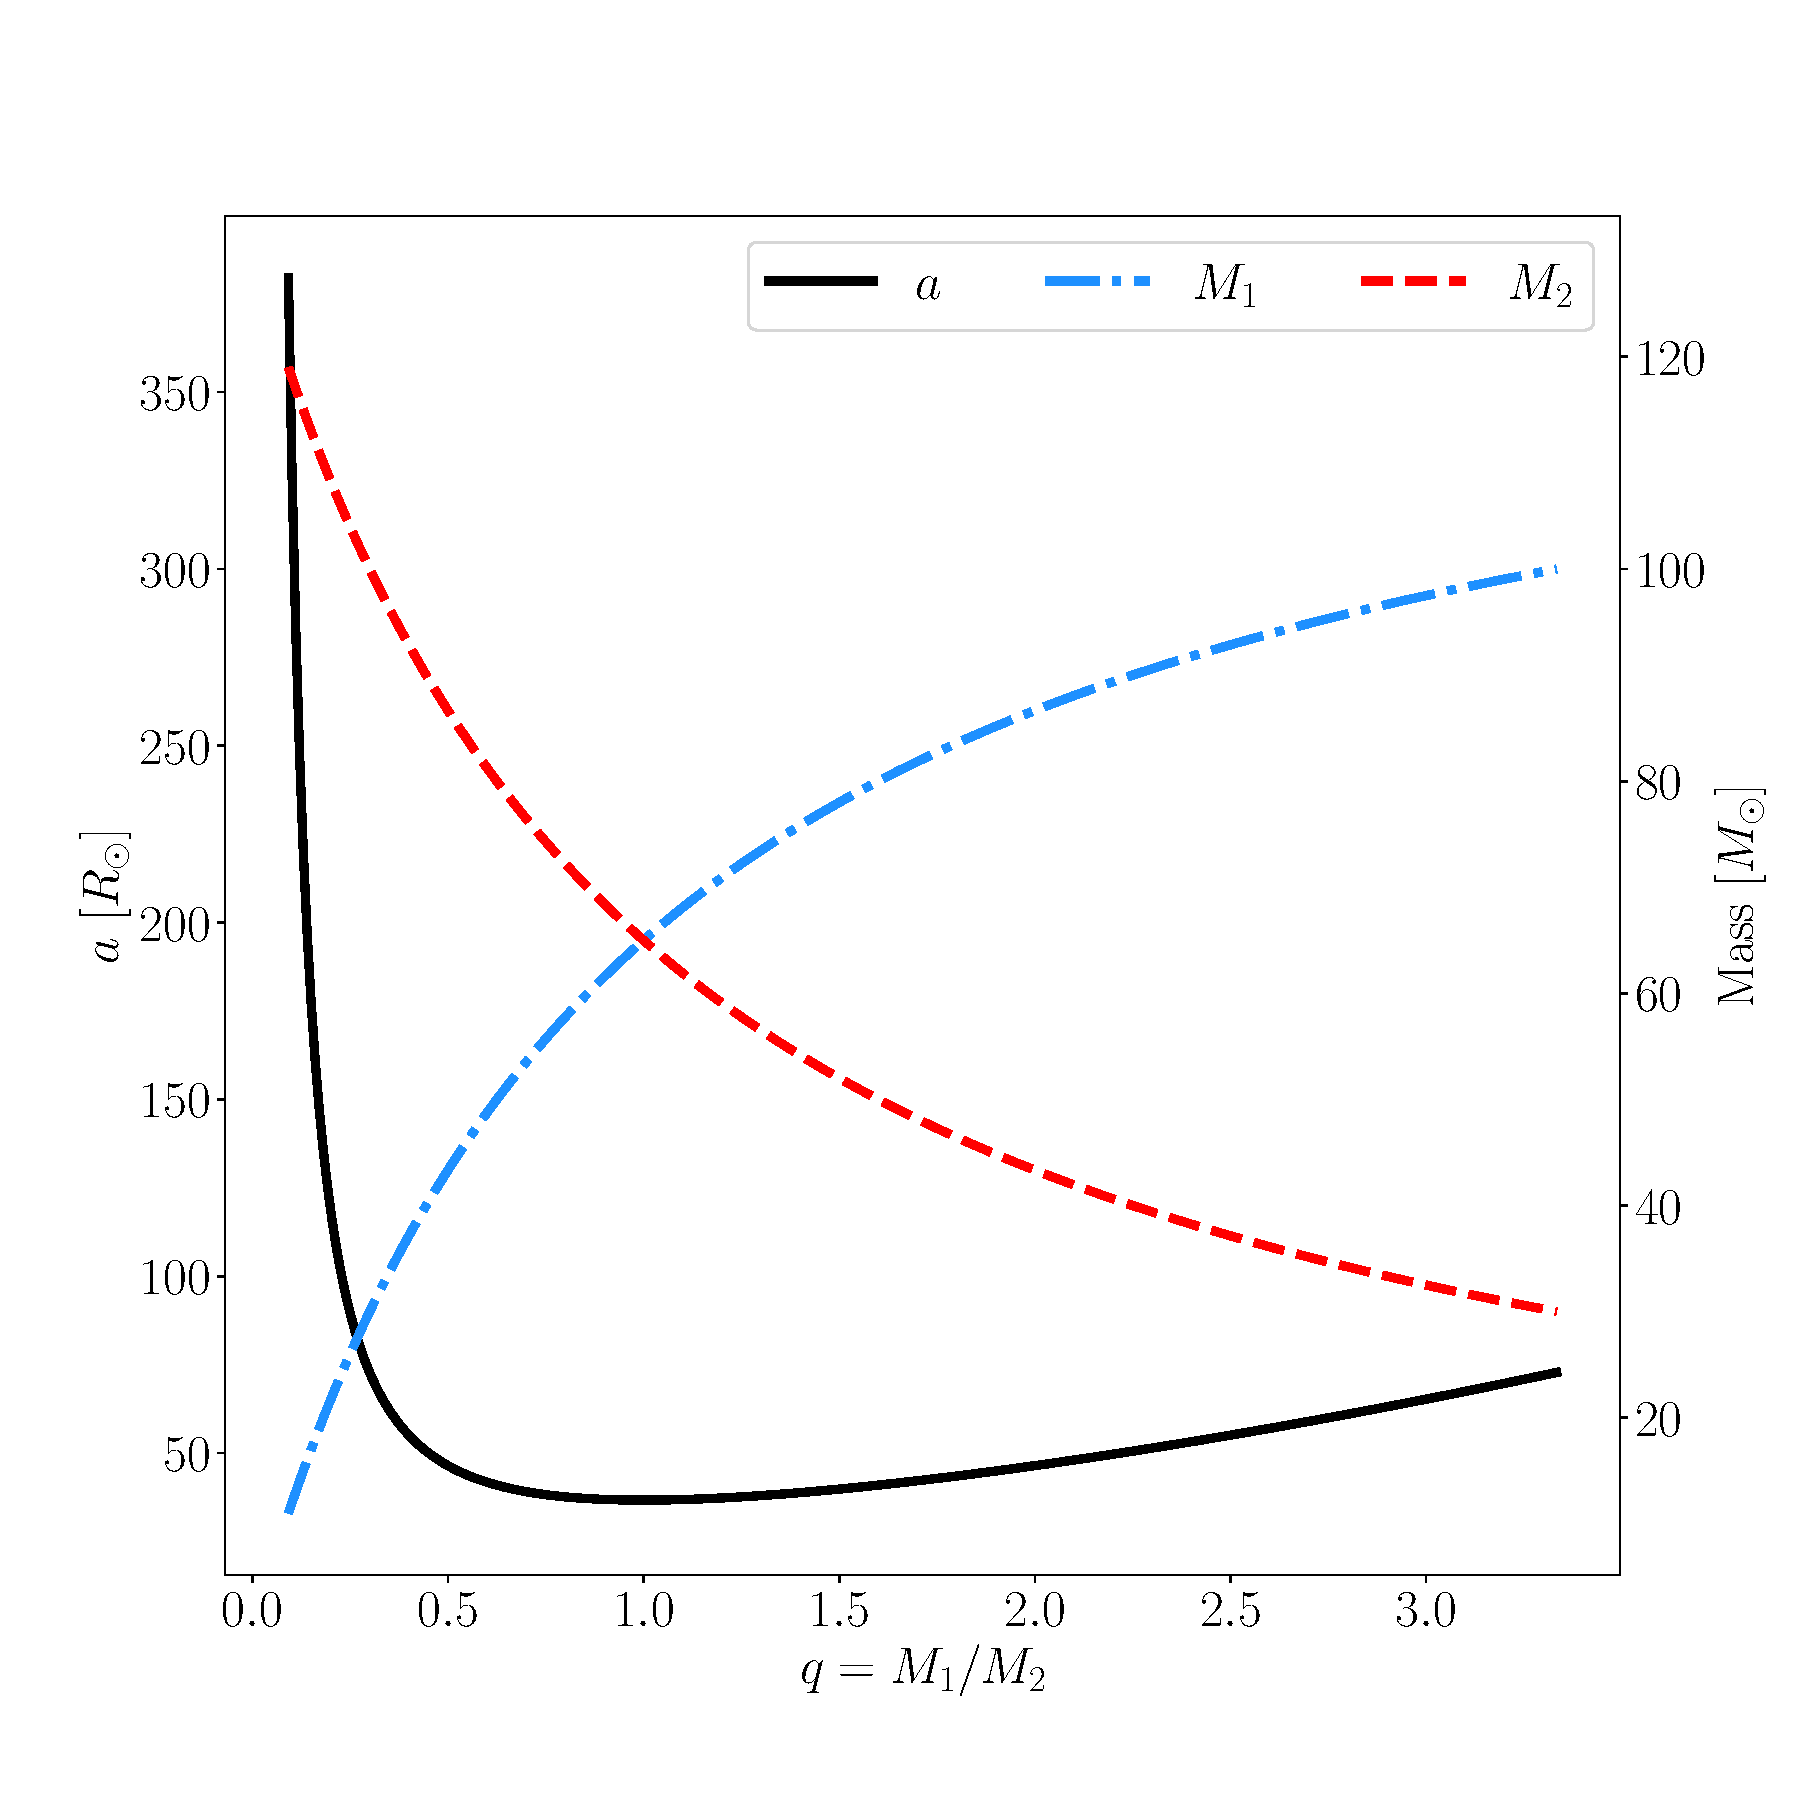
\includegraphics[width=\textwidth]{./images/masstransfer.pdf}
	\end{minipage}
	\hfill
	\begin{minipage}{.44\textwidth}
		\centering
		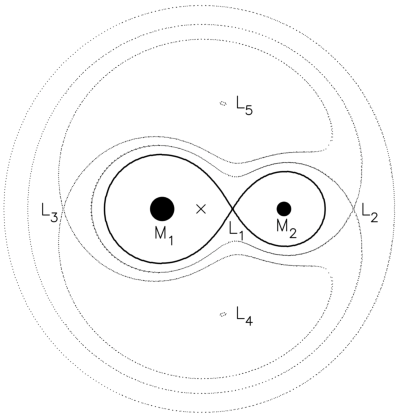
\includegraphics[width=\textwidth]{./images/Rochepotential.pdf}	
	\end{minipage}
	\caption{\emph{Left:} Conservative mass transfer from $M_1$ to $M_2$ first shrinks the semi-major axis of the orbit $a$ and then, when the secondary star becomes more massive than the primary $M_2 \geq M_1$, the orbit widens (see Eq.\ \ref{eq:a_const}). \emph{Right:} Orbital plane section of the equipotential curves of the Roche potential in the frame co-rotating with the binary. The Roche lobe is the black thick line containing the Lagrangian point $L_1$ \cite{tauris_evo_binaria}.}\label{fig:masstransferRochelobe}
\end{figure}

\subsection{Wind-fed binaries}\label{subsec:windfed}
Stellar winds cause an isotropic spread of the mass lost by the primary $M_1$, thus, it is reasonable to consider the secondary star $M_2$ as orbiting in a gas cloud. If the orbital velocity $v_{\rm orb}$ is small compared to the wind velocity $v_w \gg v_{\rm orb}$, accretion can be assumed spherical and described with the Bondi-Hoyle formalism \cite{BondiHoyle1944}: the average mass accreted over an orbital period by the secondary is

\begin{equation}\label{eq:accretionbondihoyle}
\langle \dot{M_2} \rangle = \frac{1}{\sqrt{1-e^2}} \left(\frac{G M_2}{v_w^2}\right)^2 \frac{\alpha_w}{2 a^2} \frac{1}{\left(1+v^2\right)^{3/2}} \dot{M_1},
\end{equation}

where $e$ is the eccentricity, $a$ the semi-major axis, $\alpha_w \approx 1.5$ an efficiency constant, $v$ is the ratio of the orbital velocity $v_{\rm orb}$ (calculated as in Eq.\ \ref{eq:mu_vorb}) and the wind velocity $v_w$ (calculated as the relative motion of the gas particles with respect to the secondary, proportional to the escape velocity with proportionality constant $\beta_w \approx 0.5-7$)

\begin{equation}
v = \frac{v_\textup{orb}}{v_w} \quad \quad v_w^2=2\beta_w \frac{G M_1}{R_1}
\end{equation}

Line-driven winds are one order-of magnitude faster than orbital velocities ($v_w \sim \SI{1000}{km/s}$ and $v_{\rm orb} \sim \SI{400}{km/s}$ \cite{CygX-3_Koljonen2017}): the $v$ term in Eq.\ \ref{eq:accretionbondihoyle} can be neglected and the average mass accreted becomes

\begin{equation}\label{eq:windfedaccretion}
\langle \dot{M_2} \rangle \propto \left(\frac{v_\textup{orb}}{v_w}\right)^4 \dot{M_1}
\end{equation}

The mass accretion rate scales as the fourth power of the velocity ratio; thus the efficiency of wind accretion is generally low: even enhanced mass loss of the primary $\mdot_1 \sim \SI{e-4}{\msun~\yr^{-1}}$ results in negligible accretion rates $\mdot_2 \sim \SI{e-8}{\msun~\yr^{-1}}$. Nevertheless, similar accretion rates are close to the ones allowed by Eddington-limited accretion onto compact objects (see Sec.\ \ref{subsec:conservativeMT}) and, even if small, are sufficient to power the formation and emission of the accretion disks in many X-ray binaries.

\subsection{Roche lobe overflow}\label{subsec:Rochelobeoverflow}
\paragraph{The Roche potential}
In the frame co-rotating with the binary, the sum of the gravitational and centrifugal potential is called Roche potential and its equipotential curves are shown in the right-hand panel of Fig.\ \ref{fig:masstransferRochelobe}. The potential wells of the stars become drop-shaped because of the orbital motion and are called Roche lobes. In order to describe them, in 1983 Eggleton \cite{Eggleton1983} introduced the Roche lobe radius $\rl$ as the radius of a sphere with volume equivalent to the one enclosed by a Roche lobe 

\begin{equation}\label{eq:rocheloberadius}
\rl = \frac{0.49~q^{2/3}}{0.6~q^{2/3} + \ln \left(1+q^{1/3}\right)}~a,
\end{equation}

where $a$ is the semi-major axis of the system and $q=M_1/M_2$ ($q=M_2/M_1$) is the ratio between the mass of the star belonging to the lobe $M_1$ ($M_2$) and its companion $M_2$ ($M_1$). The formula is obtained assuming circular and synchronized orbit, a condition often true for mass-transferring systems where tight orbits are rapidly circularized and synchronized by tides.

\paragraph{Stability of the Roche lobe overflow} When a star expands beyond its Roche lobe (for instance because of stellar evolution or because the orbit shrinks), the layers outside the Roche lobe are no more bound to the star's potential well and can either be lost by the binary or accreted by the companion in the so-called Roche lobe overflow (RLO) process. The stability and efficiency of the RLO are still poorly understood and provide an active field of research because they depend on many factors, like the presence of a convective or radiative envelope and a core more or less prominent (both determine the response of the star to the removal of the external envelope) or the possibility that the mass is transferred also from the external atmosphere of the star and outflows from the outer Lagrangian point of the donor (both determine the mass loss rate) \cite{marchant2021_masstransferMESA}.\\

A star that loses its external layers needs to re-adjusts its dimension in order to return to an equilibrium state. If the new equilibrium is achieved with a stellar radius still larger than the Roche lobe radius, the star will keep losing its outer layers in an unstable runaway that will lead the system to a common envelope (see Sec.\ \ref{subsec:Commonenvelope}). In contrast, if the star returns to the equilibrium state inside the Roche lobe, the RLO ends in a stable way. In this case, stellar evolution may stimulate further expansion (for instance, during the Hertzsprung-gap phase or by igniting the core He-burning, as described in Sec.\ \ref{subsec:stellarevo}): the star can undergo a series of stable RLOs and transfer a large amount of mass. For instance, Hurley et al.\ \cite{Hurley2002} proposed that stable RLO would lead to a mass loss rate scaling as the amount of Roche lobe overfilling 

\begin{equation}\label{eq:masslostRoche}
    \mdot_1 \propto \left[ \ln \left(\frac{R_1}{\rlone} \right)\right]^3
\end{equation}

RLOs can be unstable over dynamical or thermal timescales, if the mass loss perturbs the hydrostatic or thermal equilibrium, respectively (see Sec.\ \ref{subsec:stellarevo}). As suggested by Webbink in 1984 \cite{Webbink1984_CE}, the (in)stability can be studied assuming that the radius is only a function of the mass $R\propto M^{\zeta}$ and, thus, comparing the logarithmic variation of the Roche lobe ($\zeta_L$) with the one induced in the stellar radius over the dynamical\footnote{The subscript ``ad'' of $\zeta_{\rm ad}$ indicates that dynamical perturbations act so rapidly that can be modelled as adiabatic processes.} ($\zeta_\textup{ad}$) or thermal ($\zeta_\textup{th}$) timescale

\begin{equation}\label{eq:zetaRLO}
\zeta_L = \frac{d \ln r_L}{d \ln M} \quad \zeta_\textup{ad} = \left(\frac{d \ln R}{d \ln M}\right)_\textup{ad} \quad \zeta_\textup{th} = \left(\frac{d \ln R}{d \ln M}\right)_\textup{th}.
\end{equation}

The most rapid variation determines the dominant perturbation timescale, thus the reference mass-radius exponent $\zeta_* = \min\{\zeta_\textup{ad},\zeta_\textup{th}\}$ that, once compared to the Roche lobe variation $\zeta_L$, defines a Roche lobe overflow to be

\begin{equation}
\begin{cases}
\text{stable} &  \zeta_* \geq \zeta_L \\
\text{unstable} &  \zeta_* \leq \zeta_L
\end{cases}
\end{equation}

Inequality signs are a consequence of the negative denominators: the variation of the Roche lobe radius is referred to stars that are \emph{losing} mass ($d \ln M \leq 0$). As a reference, the left-hand panel of Fig.\ \ref{fig:RLOstability} shows a qualitative comparison between mass transfer episodes that are stable ($\zeta_* \geq \zeta_L$, S point), unstable on a thermal timescale but stable on the dynamical one ($\zeta_\textup{th} \leq \zeta_L \leq \zeta_\textup{ad}$, T point) or unstable on a dynamical timescale ($\zeta_\textup{ad} \leq \zeta_L$, P point).

\paragraph{Role of stellar envelope, core size and mass ratio} The convective or radiative nature of the envelope strongly affects the re-adjustment in the stellar structure after the removal of an external layer, eventually determining stability and efficiency of the RLO. Radiative envelopes have a steep density gradient that prevents the onset of convection: the pressure exerted by the outer layers is so small that, once they are removed, the star almost does not need to expand to restore the equilibrium. Thus, stars with radiative envelopes have final radii usually lower than the initial ones ($\zeta_{\rm {ad}} \gg 0$) and will likely undergo stable RLOs. Convective envelopes, on the contrary, have an adiabatic structure that almost restores the initial radius via adiabatic expansion ($\zeta_{\rm {ad}} \lesssim 0$): similar stars will likely still overfill their Roche lobe after their re-adjustment and will enter unstable RLO \cite{binaries} .\\

Stars that have a convective envelope and a central core or that are fully convective have been often modelled with  \emph{condensed} or \emph{complete} polytropes\footnote{Convective envelopes, or full stars for the complete polytrope case, were modelled with a polytropic index $n=3/2$.}, respectively, because of limited computational power. In 1987, Hjelliming \& Webbink used polytropic models to study RLO instability on the dynamical timescale, finding that the core, when is present, increases the convective efficiency of the external envelope: stars lose more energy and reduce their radius as shown in the right-hand panel of Fig.\ \ref{fig:RLOstability}, likely avoiding an unstable RLO. The more evolved the star is, the more the core becomes important in the structure: it grows in size and mass fraction because of the advanced nuclear burning and of the removal of the external layers (caused by stellar winds and previous mass transfer episodes) \cite{hjellmingwebbink1987_coreRLOF} .\\

The binary mass ratio $q$ is another factor influencing the RLO stability, since it enters the Roche lobe radius definition of Eq.\ \ref{eq:rocheloberadius}. As shown in the right-hand panel of Fig.\ \ref{fig:RLOstability}, a donor star $M_1$ much more massive than the companion $M_2$ ($q=M_1/M_2 \gg 1$) transfers a lot of mass and causes a rapid expansion of the companion potential well, thus shrinking its own Roche lobe and facilitating the onset of an unstable RLO. In contrast, stars with similar masses have similar Roche lobes with sizes modulated by the semi-major axis: assuming, as a reference, a conservative mass transfer as the one shown in the left-hand panel of Fig.\ \ref{fig:masstransferRochelobe}, systems with $q \sim 1$ have negligible changes in the semi-major axis extent, thus in the Roche lobe sizes. \\

\begin{figure}
	\begin{minipage}{.49\textwidth}
		\centering
		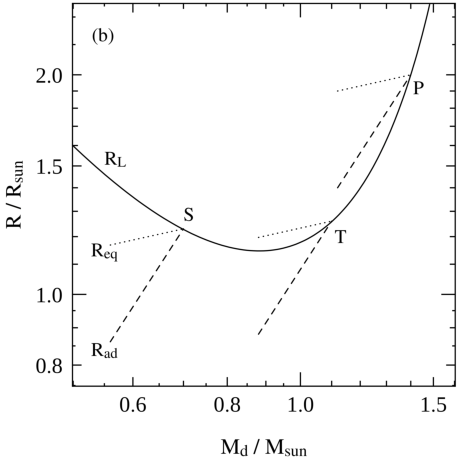
\includegraphics[width=\textwidth]{./images/stp_roche.pdf}
	\end{minipage}
	\hfill
	\begin{minipage}{.49\textwidth}
	    \vspace{-7mm}
		\centering
		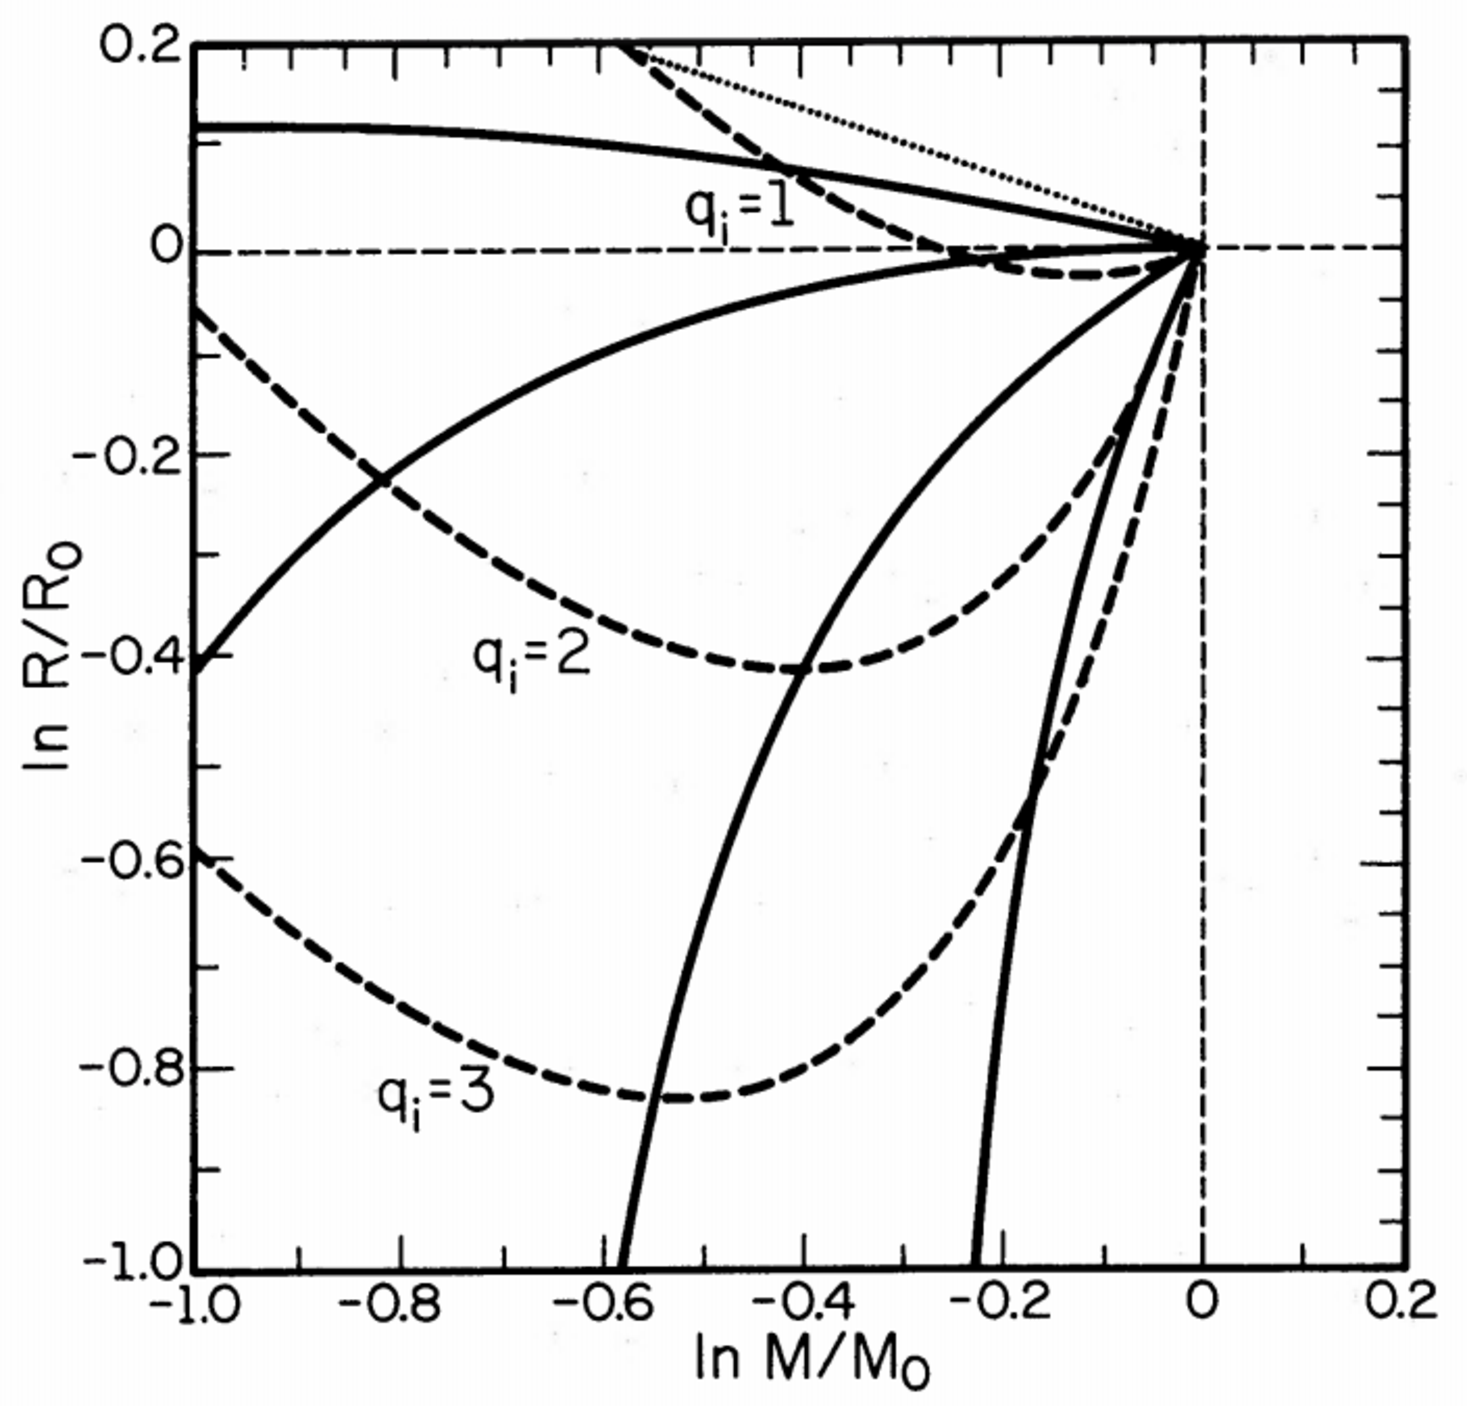
\includegraphics[width=\textwidth]{./images/core_he_rlof.pdf}	
	\end{minipage}
	\caption{\emph{Left:} Examples of the RLO (in)stability scenarios for a $\SI{2}{\msun}$ binary with fixed donor mass-radius exponents ($\zeta_\textup{ad}=1.5$ and $\zeta_\textup{th}=\zeta_\textup{eq}=0.25$, illustrated  by the dashed and dotted lines, respectively). Different donor masses determine different Roche lobe radii (solid line, Eq.\ \ref{eq:rocheloberadius}), thus the same adjustment to the mass loss ($\zeta_*$) might determine a RLO stable ($\zeta_* \geq \zeta_L$, S point), stable on the dynamical timescale but unstable on the thermal one ($\zeta_\textup{th} \leq \zeta_L \leq \zeta_\textup{ad}$, T point) or unstable also on the dynamical timescale ($\zeta_\textup{ad} \leq \zeta_L$, point P) \cite{binaries}. \emph{Right:} Adiabatic variation of the stellar radius as a function of the mass lost ($R_0$ and $M_0$ are the values before mass loss). Solid lines: condensed polytropes with growing core sizes (from top to bottom $q_\textup{core}$=0.10, 0.25, 0.50, 0.75). Dotted line: complete polytrope, models a fully convective star with $n=3/2$. Dashed lines: Roche lobe radii for different initial mass ratios (from top to bottom $q_i=M_{\rm don}/M_{\rm acc}=1,2,3$). A convective star may avoid a dynamically unstable RLO if it has a prominent core $q_{\rm core} \gg$ or it has a companion with similar mass $q \sim 1$ \cite{hjellmingwebbink1987_coreRLOF}.}\label{fig:RLOstability}
\end{figure}


Many works in the literature started from the above considerations to obtain models and thresholds that could numerically determine whether or not a binary system would enter a stable or unstable mass transfer. Similar models often are too much simplified and calibrated on old stellar tracks (or even to polytropes) but provide a fast and easy-to-implement method to calculate the RLO (in)stability in population-synthesis codes. For instance, many codes (including the one adopted in this thesis, \texttt{SEVN} \cite{spera2019_mergingBBH}) derived part of their mass transfer prescriptions from the formalism suggested by Hurley et al.\ for the \texttt{BSE} code \cite{Hurley2002}. These codes assume a one-to-one correspondence between the burning stage, the radiative/convective nature of the envelope and the core size, starting a RLO unstable on the dynamical timescale when the mass ratio $q=M_{\rm donor}/M_{\rm accretor}$ is larger than a given threshold $q_{\rm crit}$, calibrated with stellar evolution models and function of the core size $q_{\rm core}=M_{\rm core, donor}/M_{\rm donor}$

\begin{equation}\label{eq:qcrit}
	q \geq q_\textup{crit} \left(q_\textup{core}\right)
\end{equation}

Unfortunately, recent studies pointed out that there is not an unique correlation between the burning stage, the extent of the radiative/convective envelope, the core size and the RLO (in)stability \cite{klencki2020_mtproblems}. Moreover, many of the values for the $q_{\rm crit}$ and mass loss rates (like the one of Eq.\ \ref{eq:masslostRoche}) were obtained from old stellar tracks (or polytropic models) that did not properly model the more massive stars, suggesting that an updated and corrected modelling of the mass transfer that accounts for up-to-date stellar evolution is required.



\subsection{Common envelope}\label{subsec:Commonenvelope}
\paragraph{A key-process in binary evolution} Stars that enter an unstable RLO (see Sec.\ \ref{subsec:Rochelobeoverflow}), collide\footnote{Collisions occur for two stars larger than the orbital separation at periastron $R_1 + R_2 > (1-e)~a$.} or are part of a contact binary\footnote{Contact binaries form when both stars overfill their Roche lobes $R_1 \geq \rlone$ and $R_2 \geq \rltwo$.} will likely share a part or all of their envelopes (if present) and enter in a \emph{common envelope} (CE) configuration. Friction due to stellar cores orbiting around each other in a medium denser than the interstellar one causes orbital orbital angular momentum and energy losses: the orbit shrinks while the gas heats up and eventually is dispersed.  Depending on the initial orbital energy, envelope potential energy and efficiency in the energy and angular momentum transfer, binaries can either spiral-in and merge or be able to eject the common envelope: in the latter case, only the nuclei survive and the orbit tightens.

Common envelope processes shrink efficiently the orbits and are determinant to form tight compact object binaries that can merge via emission of gravitational waves within a Hubble time \cite{spera2019_mergingBBH}. However, only systems with the right combination of stellar and orbital properties can survive to common envelopes events. For instance, the orbit must be wide enough not to merge too rapidly and both stars should have a well-developed core: the latter condition prevents the core mass to be transferred into the common envelope and allows the star to survive as a self-gravitating object. A summary of the main formation channels and outcomes of the CE evolution is shown in Fig.\ \ref{fig:ce_mapelli}.

It is important to point out that evolution through a CE phase efficiently removes the hydrogen envelope of one or both stars. Therefore, common envelope is a key-process to form Wolf-Rayet stars and its role will be further discussed in the results of this thesis, presented in Sec.\ \ref{sec:results}.


\begin{figure}
	\centering
	\def\svgwidth{0.9\textwidth}
	\import{./images/}{ce_schema.pdf_tex} 
	\caption{Possible initial and final common envelope configurations. The two stars are represented with cores (blue for the primary, black for the secondary) and envelopes (orange) but it could also be that one of the two stars has not yet developed a core (e.\ g.\ a MS star), is already envelope-stripped (e.\ g.\ a Wolf-Rayet star) or is a compact object (e.\ g.\ a black hole). A binary may enter a CE after an unstable RLO, a collision, or after being a contact binary. The H-rich envelope of one or both stars are shared and if at least one of the stars %is missing a 
	does not have a core, the two are merged. In contrast, the two nuclei (or a nucleus/Wolf-Rayet  star and a compact object) could survive the spiral-in if the initial orbit is wide enough to eject the envelope, heating the gas through friction. The scheme is inspired by figure no. 7 of Mapelli \cite{mapelli} and implements the standard cases for common envelope evolution. The \texttt{SEVN} version adopted in this thesis, however, avoids the creation of over-contact binaries in order to reproduce the observed neutron stars merger rates (see Sec.\ \ref{subsec:masstransferSEVN} and Iorio et al.\ in preparation).}\label{fig:ce_mapelli}
\end{figure}


\paragraph{$\boldsymbol{\alpha \lambda}$ formalism} The most widely adopted description for common envelope processes is the bi-parametric one proposed by Webbink in 1984 \cite{Webbink1984_CE}. They assume that orbital energy is the only energy source to power the envelope removal and they model the energetic balance with two adimensional parameters: $\alpha$ and $\lambda$.

The $\alpha$ parameter indicates the fraction of orbital energy  $E_{\rm orb}$ used to eject the common envelope

\begin{equation}\label{eq:EorbCEalpha}
\Delta E_\textup{orb} = \alpha \left(E_\textup{orb, f} - E_\textup{orb, i}\right) = \alpha \frac{G M_\textup{c,1} M_\textup{c,2}}{2} \left(\frac{1}{a_\textup{i}} - \frac{1}{a_\textup{f}}\right),
\end{equation}

where $M_\textup{c,1}$ and $M_\textup{c,2}$ are the two core masses and $a_\textup{i}$ and $a_\textup{f}$ are the initial and final semi-major axis, respectively . Because of friction, the orbit shrinks, thus $a_\textup{f} < a_\textup{i}$ and $\Delta E_\textup{orb} \leq 0$.

The $\lambda$ parameter is related to the common envelope concentration: small values of $\lambda$ indicate concentrated envelopes, more difficult to eject. In particular, $\lambda$ is related to the envelope binding energy of the single stars through dimensional considerations

\begin{equation}\label{eq:EenvCElambda}
E_\textup{env} = - \frac{G}{\lambda} \left(\frac{m_\textup{env,1} M_1}{R_1}+ \frac{m_\textup{env,2} M_2}{R_2}\right)
\end{equation}

where $R$, $M$ e $m_\textup{env}$ are respectively radius, mass and envelope mass of each star at the onset of common envelope.

Imposing that the orbital energy lost by the system equals the common envelope binding energy ($\Delta E_\textup{orb} = E_\textup{env}$), it is possible to obtain the system final semi-major axis as function of the $\alpha$ and $\lambda$ parameters

\begin{equation}\label{eqn:a_ce}
\frac{1}{a_\textup{f}} = \frac{1}{\alpha \lambda} \frac{2}{M_\textup{c,1} M_\textup{c,2}} \left(\frac{m_\textup{env,1} M_1}{R_1}+ \frac{m_\textup{env,2} M_2}{R_2}\right) + \frac{1}{a_\textup{i}}
\end{equation}

The direct proportionality $a_\textup{f} \propto \alpha\lambda$ indicates that binaries with more chances of survival are the ones that have poorly concentrated envelopes and efficiently converted the orbital energy into heat. \\

Even though the $\alpha \lambda$ formalism is easy-to-implement and widely adopted in population-synthesis codes, there is general consensus in the literature that it needs to be updated with a more detailed and self-consistent treatment of stellar and binary evolution \cite{marchant2021_masstransferMESA}. Many observed systems suggest that likely $\alpha > 1$, meaning that additional forms of energy need to be considered to eject the common envelope \cite{mapelli}. Moreover, current implementations adopt $\lambda$ values obtained from fits to various stellar evolution models even though  a self-consistent calculation should be preferred. In particular, fits to single stellar evolution tracks do not account for changes in the binding energy due to mass transfer events and their result are sensitive to the internal energy sources considered. For instance, Marchant et al.\ \cite{marchant2021_masstransferMESA} pointed out that fits from Claeys et al.\ \cite{Clayes2014_lambdaCE}, widely implemented in population-synthesis codes (including the one adopted in this thesis, \texttt{SEVN}, see Sec.\ \ref{subsec:masstransferSEVN}), underestimate the binding energy of stars that frequently enter a common envelope, like Hertzsprung-gap stars, overestimating the number of systems that survive to it and, eventually, merge as binary black holes. 


Recently, Gallegos-Garcia et al.\ \cite{gallegos2021MESAvspopsynth} further demonstrated that, at least for H-rich donor stars, current prescriptions for entering an unstable RLO and surviving the common envelope may overestimate  the binary black hole merger rates by a factor $\sim 5-500$, favouring too much the formation through common envelope evolution in systems that, instead, likely evolve through stable RLOs as shown in Fig.\ \ref{fig:MESAvsPopsynth}.

\begin{figure}[h!]
		\centering
		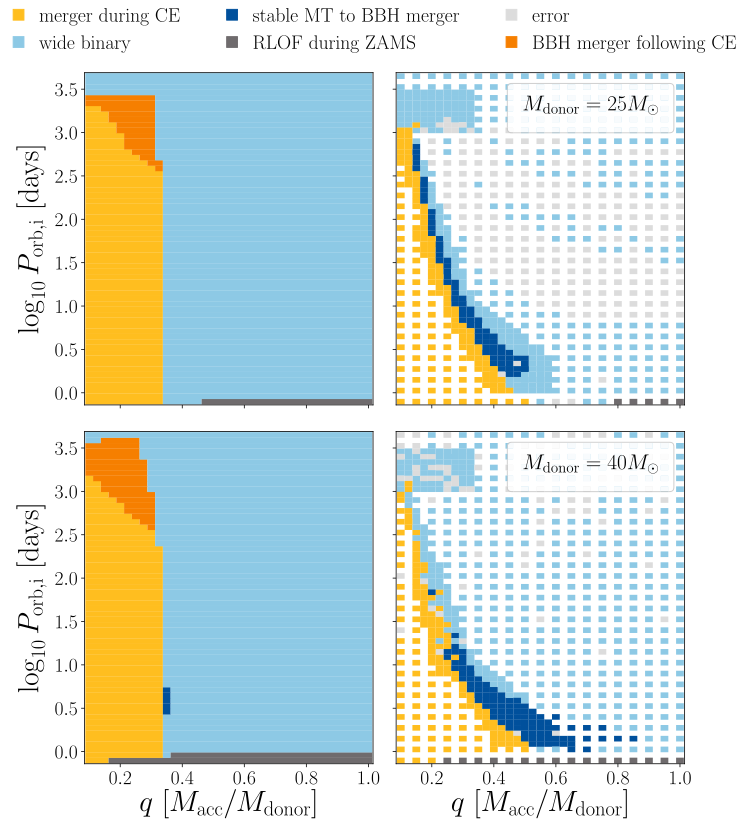
\includegraphics[width=0.9\textwidth]{./images/MESAvspopsynth.png}	
	\caption{Comparison of final outcomes for the same initial binary population evolved with the \texttt{COSMIC} population-synthesis code \cite{breivik2020cosmicpopsynth} (\emph{left}) and with the \texttt{MESA} stellar evolution code, which also implements modules for binary evolution \cite{MESA2015BinaryMT} (\emph{right}). Each row shows the initial period as a function of the initial mass ratio for H-rich donors of $M = 25~\msun$ (top) and $M = 40~\msun$ (bottom) at sub-solar metallicity $Z=0.00142$. On-the-fly stellar and binary evolution carried out in \texttt{MESA} suggests that only a restricted parameter space region successfully forms binary black holes (BBHs), in contrast with results from population-synthesis codes. \texttt{MESA} BBHs formed mainly through stable RLO, whereas CE evolution dominated for \texttt{COSMIC} BBHs \cite{gallegos2021MESAvspopsynth}.}\label{fig:MESAvsPopsynth}
\end{figure}




\section{Observed candidates of Wolf-Rayet -- black hole systems}\label{sec:WRBHobserved}

\subsection{Overview of WR--BH properties and fates}
We know of only seven candidate Wolf-Rayet -- black hole binaries (hereafter, WR--BH): their main parameters and uncertainties are listed in Tab.\ \ref{tab:observations} \cite{observations}. General properties of WR--BH systems are presented in this section, while in the next ones I will discuss the characterization of each system.


\paragraph{Masses and periods} As explained in Sec.\ \ref{subsec:Xraymeasure} and Sec.\ \ref{subsec:massWR}, X-ray light curves and UV, optical, near-IR spectra are the main tools used to characterize stellar and binary properties. While they provide precise estimates of the orbital period, the masses are often so poorly constrained that it is not possible to determine whether some compact objects are neutron stars or black holes, although further X-ray observations suggest a mild preference for a black hole in Cyg X-3 and IC10 X-1. 

Spectroscopic analysis ensured the Wolf-Rayet nature of the companions in Cyg X-3, IC10 X-1, NGC300 X-1 and M101 ULX-1. In contrast, CXOU J123030.3+413853, CXOU J004732.0-251722.1 and CG X-1 are more uncertain as WR--BH binaries and their classification is based only X-ray measurements, since spectroscopic observations were not available.  Moreover, the uncertain candidates belong to starburst galaxies, further supporting the possibility of being at least high-mass X-ray binaries (HMXBs, see Sec.\ \ref{subsec:cygx3observations}, \ref{subsec:IC10X1_revisedmasses}, \ref{subsec:uncertainWRcandidates} for a detailed discussion on the single system properties).


%%%%%%%%%%%%%%%%%%%%%%%%%%
%%%%%%%%%%%%%%%%%%%%%%%%%
\begin{figure}[b!]
    \centering
	\begin{threeparttable}
		\begin{tabular}{llcccccc}
			\toprule
			\multirow{2}{*}{Host galaxy} & \multirow{2}{*}{Name} & $M_{\rm BH}$ & $M_{\rm WR}$ & $P$ & $t_\textup{GW}$  &  Z & $d$ \\
			& & [$\msun$] & [$\msun$] & [hours] & [Gyr] & [$\zsun$] & [Mpc]\\
			\midrule
			Milky Way & Cyg X-3 & 3-10 \tnote{a} & 8-14 \tnote{a} &4.8 \tnote{b} & 0.02 & 0.92 & 0.00741 \\
			IC 10 & IC10 X-1 & - \tnote{c} & 17-35 \tnote{d} & 34.9 \tnote{e} & 3.5  & 0.22 & 0.70\\
			NGC 300 & NGC300 X-1 & 13-21 \tnote{f} & 15-26 \tnote{g} & 32.8 \tnote{f} & 2.9  & 0.19 & 2.02\\
			NGC 253 & CXOU J004732.0-251722.1 & - & - & 14.5 \tnote{h} & 0.3  & 0.24 & 3.0 \\
			Circinus & CG X-1 & - & - & 7.2 \tnote{i}  & 0.05 & 0.10 & 4.2 \\
			M101 & M101 ULX-1 & 8-46 \tnote{j} & 17-19 \tnote{j} & 196.8 \tnote{j} & 348 & 0.17 & 6.9\\
			NGC 4490 & CXOU J123030.3+413853 & - & - & 6.4 \tnote{k} & 0.04  & 0.23 & 8.55\\
			\bottomrule 	
		\end{tabular}
		\begin{tablenotes}[para]
		    \item[a]\cite{CygX-3_Koljonen2017} 
		    \item[b]\cite{CygX-3_Singh2002} 
			\item[c]\cite{ICX10X-1_Laycock2015_revisited} 
			\item[d]\cite{IC10X-1_Clark2004_WRmass}
			\item[e]\cite{IC10X-1_Silverman2008} 
			\item[f]\cite{NGC300X-1_Binder2021_BHpreciso}
		    \item[g]\cite{NGC300X-1_Crowther2010} 
		    \item[h]\cite{NGC253cand_Maccarone2014} 
		    \item[i]\cite{observations}
		    \item[j]\cite{M101ULX-1_Liu2013} 
		    \item[k]\cite{NGC4490cand_Esposito2013c} 
		\end{tablenotes}
	\end{threeparttable}
	\captionof{table}{Properties of the seven WR--BH candidates. Table inspired by \cite{observations}. Masses and periods are extracted from papers referenced with the superscripts and discussed in Sec.\ \ref{subsec:cygx3observations}, \ref{subsec:IC10X1_revisedmasses}, \ref{subsec:uncertainWRcandidates}. $t_\textup{GW}$ is an order-of-magnitude estimate for the merger time via gravitational-wave emission and is calculated with Eq.\ \ref{eq:tgw} assuming the same observed period and $M_{1,\rm BH} = M_{2,\rm BH} = 10~\msun$, given the uncertainties in the mass determination discussed in Sec.\ \ref{sec:WRBHobserved}. Distances and metallicities refer to the host galaxies as in \cite{observationsZSFR_Mapelli2010a} for all binaries except for Cyg X-3: its distance is taken from \cite{CygX-3_McCollough2016_Observation} and is used to infer the local metallicity from the Milky Way metallicity gradient \cite{MetallicityGradientMW2018Gaia}, as explained in Sec.\ \ref{subsec:cygx3observations}.} \label{tab:observations}
\end{figure}
%%%%%%%%%%%%%%%%%%%%%%%%%
%%%%%%%%%%%%%%%%%%%%%%%%%

\paragraph{Fates} Even though the mass estimates are quite uncertain, all the considered Wolf-Rayet stars are massive enough to collapse into a black hole: the observed WR--BHs are likely progenitors of binary black holes (see Sec.\ \ref{subsec:stellarevo}). Using the formula derived in 1964 by Peters \cite{Peters1964}, it is possible to obtain an order-of-magnitude estimate for the time needed to merge via GW emission $t_\textup{GW}$:

\begin{equation}\label{eq:tgw}
t_\textup{GW} = \frac{5}{256} \frac{c^5\,{} a^4 \,{}(1-e^2)^{7/2}}{G^3\,{} M_1\,{} M_2\,{} (M_1 + M_2)},
\end{equation}

where $G$ is the gravitational constant, $c$ is the speed of light, and $a$ is the semi-major axis. For simplicity, it is reasonable to assume that the orbital period of the binary black hole will be similar to the one observed in the WR--BH configuration (simulated systems discussed in Sec.\ \ref{sec:results} show that the WR--BH period is indeed little affected by the supernova kick and remains almost identical when a binary black hole forms). Following \cite{observations}, the reference compact object binary is assumed to have circular orbit (eccentricity $e=0$), secondary BH of $M_{2,\rm BH} \sim 10~\msun$ produced by the WR and primary BH of $M_{1,\rm BH} \sim 10~\msun$. Such masses are probably smaller than the real ones but allow to obtain an upper boundary for $t_\textup{GW}$. Under these assumptions, WR--BH systems need to have a period $P \lesssim 10~$ days ($a \lesssim 20~\rsun$) in order to merge within a Hubble time. By comparing this value with the ones reported in the Table \ref{tab:observations}, all binary systems formed with characteristics similar to the observed WR--BH candidates could produce a merging binary black hole observable today, with the exception of systems like M101 ULX X-1, that are too wide to merge within a Hubble time. However, these are only approximated conclusions because the approach adopted here neglects the impact of any possible natal kicks.


\subsection{Cyg X-3}\label{subsec:cygx3observations}
Cyg X-3 is the only known WR--BH candidate in the Milky Way: being at almost solar metallicity, it will become a case-study binary in this thesis work and its possible evolutionary pathways will be discussed in Sec.\ \ref{sec:results}. Hereafter, I will present the key observations that characterize Cyg X-3, highlighting the ones that will be used as fiducial model in this thesis.

\paragraph{Distance}
X-ray and sub-millimetric observations revealed that Cyg X-3 has a nearby Bok globule located 15.6" away from the binary, as shown in the left-hand panel of Fig.\ \ref{fig:CygX3}. This Cyg X-3 ``little friend '', as it is sometimes called, is a cloud of gas and dust of $\sim 2-24~\msun$ with $\sim 0.2$ pc diameter and is associated with a star-forming region. Observations of the 1.3 mm CO line revealed a velocity shift of $\SI{-47.5}{km/s}$. Since the cloud belongs to the Galactic plane, it is reasonable to assume that the Doppler shift is dominated by rotational velocity. However, the Bok globule is close to the Perseus arm and there have been evidences of anomalous motion of objects in that region. Thus, McCollough et al.\ \cite{CygX-3_McCollough2016_Observation} used a Bayesian tool that could account for errors in the estimated kinematic distances, finding that the Bok globule has 62 \% of probability of being at $d_{\rm Bok} = 6.08 \pm 0.64$ kpc and 38 \% probability of being at $d_{\rm Bok} = 7.85 \pm 0.6$ kpc.

X-ray light curves of this Bok globule exhibit the same period modulation of Cyg X-3 but are shifted in phase by $\Delta \phi = 0.56$, suggesting that X-ray photons emitted by the binary are scattered by the dust cloud towards the observer. The small angular separation between the Bok globule and Cyg X-3 coupled with the observed time delays allow us to use geometrical arguments to determine the distance of Cyg X-3. Using the previously determined relative distance of the Bok globule of $d_{\rm Bok} = 6.08 \pm 0.64~ (7.85 \pm 0.6)$ kpc , McCollough et al.\ found that Cyg X-3 is distant $0.82 \pm 0.09~ (0.77 \pm 0.07)$ kpc from the Bok globule and $d_{\rm Cyg~X-3} = 7.41 \pm 1.13~ (10.16 \pm 1.21)$ kpc from the observer. The first estimate relies on the most probable value for the Bok globule's distance, therefore can be used as reference value for the Cyg X-3 distance

\begin{equation}\label{eq:distanceCygX3}
    \boxed{d_{\rm Cyg~X-3} = 7.41 \pm 1.13 ~\rm kpc}
\end{equation}



Assuming that the supernova explosion that formed the compact object of Cyg X-3 occurred $\sim 1-5$ Myrs ago (average lifetime of a Wolf-Rayet, see Sec.\ \ref{subsec:stellarevo}) and that Cyg X-3 originally formed in that Bok globule, the relative distance of $\sim 1$ kpc suggests a natal kick of 190-980 km/s. Both distances and natal kick estimates are consistent with independent calculations in the literature, although the work of McCollough et al.\ provides the most precise distance determination.

\paragraph{Metallicity}
In 2018 Lemasle et al.\ \cite{MetallicityGradientMW2018Gaia} used distances and metallicities of twenty-five Cepheids from the Gaia Data Release 2 to estimate the Milky-Way metallicity gradient, finding the relation

\begin{equation}\label{eq:MWmetallicitygradient}
    [\rm Fe/H]=-0.0447~d_{\rm Gal} + 0.3522
\end{equation}

where $d_{\rm Gal}$ is the Galactocentric distance expressed in kpc units.

Assuming, as Lemasle et al.\ \cite{MetallicityGradientMW2018Gaia}, that the Sun has a Galactocentric distance of $d_{\rm \odot,Gal} = 7.94$ kpc and recalling, as McCollough et al.\ \cite{CygX-3_McCollough2016_Observation}, that Cyg X-3 lies on the Galactic plane ($l=79.84^\circ, b=+0.70^\circ$) with relative distance to the Sun of $d_{\rm Cyg~X-3} = 7.41 \pm 1.13$ kpc, I used trigonometric relations to infer the Galactocentric distance of Cyg X-3 as $d_{\rm Cyg~X-3, Gal} = 9.85$ kpc. At this distance, the metallicity of the Milky-Way estimated through the gradient of Eq.\ \ref{eq:MWmetallicitygradient} as [Fe/H] = -0.088. 

Assuming that the metallicity distribution of the Sun is universal \cite{metallicityFeHconversion}, the [Fe/H] metallicity of any star can be converted into metal mass fraction $Z$ with the relation 

\begin{equation}
    [\rm Fe/H]_* = \log(Z/X)_* - \log(Z/X)_\odot{},
\end{equation}


where $X$ is the hydrogen mass fraction. For a star at the Galactocentric distance of Cyg X-3, the metal content is thus

\begin{equation}\label{eq:CygX3metallicity}
    \boxed{Z_{\rm Cyg~X-3} = 0.916~\zsun}
\end{equation}

This metallicity is the one reported in Tab. \ref{tab:observations} for Cyg X-3 and is  very similar to the solar one, given that both the Sun and Cyg X-3 have almost the same Galactocentric distance. In particular, assuming standard solar metallicity of $\zsun =0.02$ implies $Z_{\rm Cyg~X-3} = 0.018$ while using updated determinations from Caffau et al.\ \cite{caffau2011solarmetallicity} $\zsun=0.015$ indicate $Z_{\rm Cyg~X-3}=0.014$.


\paragraph{Period} Cyg X-3 light curves and spectra exhibit a strong modulation of 4.8 hours ($\sim 4^{\rm h} 48^{\rm m}$). In particular, Singh et al.\ \cite{CygX-3_Singh2002} obtained very accurate values for period $P$ and period derivative $\dot{P}$ from parabolic fits to X-ray light curves

\begin{equation}\label{eq:periodCygX3}
    \boxed{P_{\rm Cyg~X-3} = 4^{\rm h} 47^{\rm m} 32.735^{\rm s}~\pm~0^{\rm h} 0^{\rm m} 0.008^{\rm s}}
\end{equation}

\begin{equation}\label{eq:pdotCygX3}
    \boxed{\dot{P}/P_{\rm Cyg~X-3} = (1.05 \pm 0.04) \times 10^{-6}~\yr^{-1}}
\end{equation}

As pointed out by Zdziarski et al.\ \cite{Cyg-X3_Zd2013}, the period of Cyg X-3 is unusually short for an HMXB and suggests a past spiral-in episode, likely due to a common envelope (see Sec.\ \ref{subsec:Commonenvelope}). This interpretation is supported also by the results of this thesis, as discussed in Sec.\ \ref{sec:results}.

\paragraph{Masses} So far only IR spectra are available for Cyg X-3: since the binary lies on the Galactic plane, strong interstellar absorption prevented the observation of optical and UV counterparts \cite{CygX-3_Koljonen2017}. The spectra revealed the presence of strong He I and He II lines, classifying the Wolf-Rayet star as a WNL sub-type (see Tab.\ \ref{tab:WRclassification}).\\

As explained in Sec.\ \ref{subsec:Xraymeasure} and Sec.\ \ref{subsec:massWR}, it is possible to use a mass-luminosity relation to determine the mass of a Wolf-Rayet star and then couple this information with period and maximum amplitude of the radial velocity curve to obtain the dynamical mass of the companion compact object. Zdiarski et al.\ \cite{Cyg-X3_Zd2013} used IR spectra extracted by Hanson et al.\ \cite{CygX-3_Hanson2000wrongspectrum} and mass-luminosity relations for WN stars calibrated by Nugis \& Lamers \cite{Nugis2000_WRwinds} to estimate a Wolf-Rayet mass of $\mwr = 10.3_{-2.8}^{+3.9}~\msun$ and a compact object mass of $M_C = 2.4_{-1.1}^{+2.1}$. However, Koljonen \& Maccarone \cite{CygX-3_Koljonen2017} pointed out that the spectra of Hanson et al.\ \cite{CygX-3_Hanson2000wrongspectrum} were taken in an outburst state, where the variability of 2.058 $\mu m$ He I absorption line (used to extract the radial velocity curve) was not tracing the orbital motion of the Wolf-Rayet star, but, instead, reflected the ionization structure of the wind. Similar misinterpretations occurred also for NGC 300 X-1 and IC 10 X-1 and caused a revision of their masses, as explained in more detail in the next section (Sec.\ \ref{subsec:IC10X1_revisedmasses}). \\

In 2017, Koljonen \& Maccarone \ \cite{CygX-3_Koljonen2017} extracted new IR spectra of Cyg X-3 and re-estimated its compact object mass. Assuming a distance of $d_{\rm Cyg~X-3} = 7.41 \pm 1.13~ (10.16 \pm 1.21)$ kpc from McCollough et al.\ \cite{CygX-3_McCollough2016_Observation}, they estimated the absolute K-band magnitude to be $M_K = -4.2 \pm 0.4~(-4.9 \pm 0.3)$ mag and used the \texttt{PoWR} non-LTE atmosphere models for WN stars \cite{WRnonLTEatmospheresPoWR_Todt2015} to derive a corresponding luminosity of $\log(L_{WR}/\lsun) = 5.32 \pm 0.16~(5.59 \pm 0.12)$. Gr{\"a}fener et al.\ \cite{Grafener2011_M-L_WR} extracted the mass-luminosity relations for non-homogeneous core-He burning stars showed in the left-hand panel of Fig.\ \ref{fig:MLandwinds} from stellar models also based on \texttt{PoWR}. Thus, Koljonen \& Maccarone self-consistently used the Gr{\"a}fener et al.\  mass-luminosity relations and determined the Wolf-Rayet masses to be $\mwr = 8-10~(11-14)~\msun$. The corresponding mass loss of $\mdot = (0.4-1.3) \times 10^{-5}~((0.6-2.0)\times 10^{-5})~\msun~\yr^{-1}$ is extracted from the \texttt{PoWR} models and then corrected for wind clumping. Overall, the Wolf-Rayet mass is consistent with the one found by Zdiarski et al.\ \cite{Cyg-X3_Zd2013} and, accounting for the possible errors in the distance estimates of McCollough et al.\ \cite{CygX-3_McCollough2016_Observation}, can be conservatively assumed to be

\begin{equation}\label{eq:MWRCygxX-3}
    \boxed{M_{\rm WR,~Cyg~X-3} = 8-14~\msun}
\end{equation}

As previously pointed out and further discussed in the next section, the strong helium lines in the IR spectrum are not reliable tracers of the orbital motion but rather reflect variability in the Wolf-Rayet winds. Therefore Koljonen \& Maccarone adopted a different strategy to determine the mass of the compact object in Cyg X-3. They assumed that all the isotropic wind flowing past the accretion radius of the compact object $r_{\rm acc}$ is accreted

\begin{equation}\label{eq:massaccretedBHCygX3}
    \mdot_{\rm acc} \approx \frac{\pi r_{\rm acc}^2}{4 \pi a^2} ~ \mdot{},
\end{equation}

where the semi-major axis $a$ is determined from Kepler's third law and the accretion radius $r_{\rm acc}$ is a function of the relative wind velocity at the location of the compact object $v_{\rm rel}$

\begin{equation}
    a = \sqrt[3]{\frac{P^2 \,{}G\,{} (\mwr + M_C)}{4 \pi}} \qquad \qquad r_{\rm acc} \sim \frac{2\,{} G\,{} M_C}{v_{\rm rel}^2} 
\end{equation}

Back-substituting $a$ and $r_{\rm acc}$ into Eq.\ \ref{eq:massaccretedBHCygX3} results in

\begin{equation}\label{eq:massaccreted2}
    \mdot_{\rm acc} \approx 0.0176 \times \left( \frac{1000~\rm km/s}{v_{\rm rel}} \right)^4 \left( \frac{4.8~\text{hrs}}{P} \right)^{4/3} \frac{M_C^2}{(\mwr + M_C)^{2/3}}   ~ \mdot
\end{equation}

Assuming that only the wind confined within the orbit falls to the compact object $r_{\rm acc} < a$ implies, according to Eq.\ \ref{eq:massaccretedBHCygX3}, that only <1/4 of all the mass lost by the Wolf-Rayet $\mdot$ is accreted. A similar and reasonable assumption, coupled with the well-know period of $P=4.8$ hrs \cite{CygX-3_Singh2002} and the previously estimated Wolf-Rayet mass loss rates of $\mdot = (0.4-2.0)\times 10^{-5}~\msun~\yr^{-1}$ \cite{CygX-3_Koljonen2017} reduce Eq.\ \ref{eq:massaccreted2} into a simple relation between the two masses and the relative wind velocity $v_{\rm rel}$, showed in the right-hand panel of Fig.\ \ref{fig:CygX3}. 

$v_{\rm rel}$ is determined by the wind terminal velocity $v_{\inf}$ and orbital velocity $v_{\rm  orb}$ through $v_{\rm rel}^2 = v_{\inf}^2 + v_{\rm orb}^2$. \texttt{PoWR} atmosphere models predict a terminal wind velocity of $v_{\inf} \approx 700-800$ km/s. In contrast, the orbital velocity is less precise $v_{\rm orb} \approx 300-750$ km/s due to the large uncertainty in the orbital inclination $i \approx 30^{\circ}-70^{\circ}$. Overall, the wind relative velocity at the compact object location is not higher than $v_{\rm rel} \lesssim 750-1000$ km/s, implying a compact object with mass $M_C \lesssim 5-10~\msun$ (see the right-hand panel of Fig.\ \ref{fig:CygX3}). 


\begin{figure}[t!]
	\begin{minipage}{.49\textwidth}
		\centering
		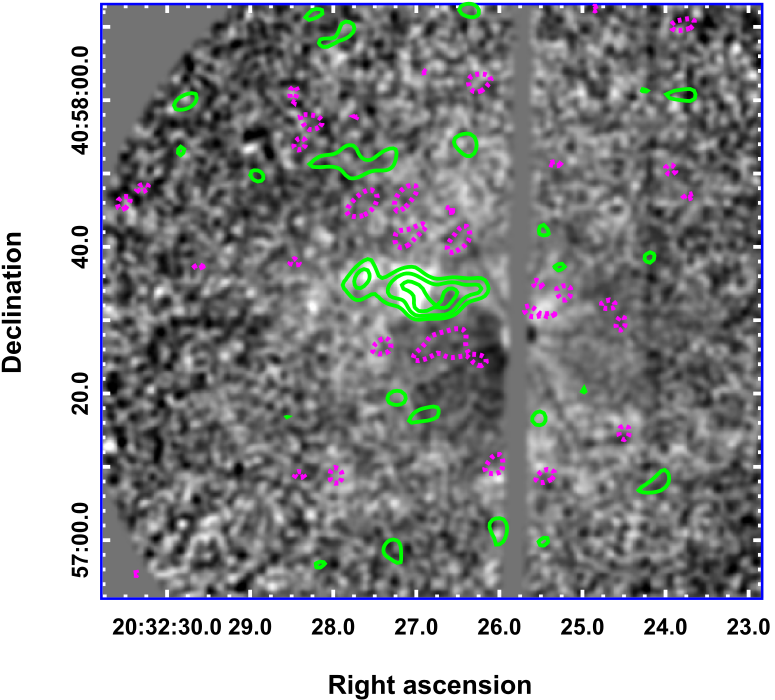
\includegraphics[width=\textwidth]{./images/CygX3littlefriend.png}
	\end{minipage}
	\hfill
	\begin{minipage}{.49\textwidth}
		\centering
		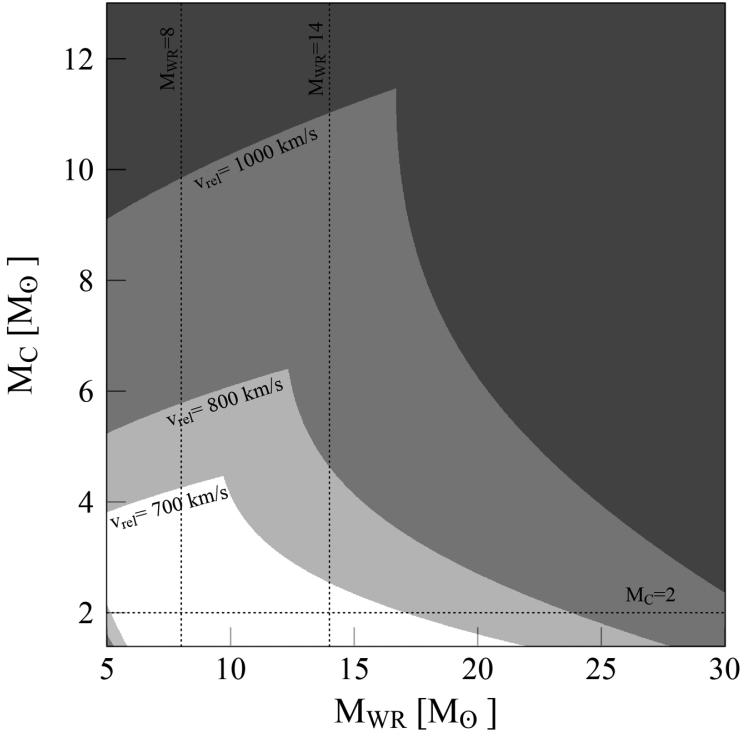
\includegraphics[width=\textwidth]{./images/CygX3massBH}	
	\end{minipage}
	\caption{\emph{Left:} Gray-scaled X-ray image of Cyg X-3 and its ``little friend''. The PSF of Cyg X-3, centered at $(\alpha \approx 26^{\rm h}, \delta \approx 30^{\circ})$, was subtracted. Sub-millimetric contours of the CO line at $-47.5$ km/s are overlaid, in green if positive and magenta if negative. The Bok globule is identified by the denser green contours superimposed to the bright X-ray blob on the left of Cyg X-3 \cite{CygX-3_McCollough2016_Observation}. \emph{Right:} Possible compact object masses $M_C$ as a function of Wolf-Rayet masses $\mwr$ with descreasing values of relative wind velocities at the location of the compact object $v_{\rm rel}$. The most probable values of $\mwr = 8-14~\msun$ and $v_{\rm rel} \lesssim 750-1000$ km/s favour a compact object with mass $M_C \lesssim 5-10~\msun$, most likely a black hole \cite{CygX-3_Koljonen2017}.}\label{fig:CygX3}
\end{figure}

\paragraph{Black hole or neutron star?}
The maximum allowed mass for a neutron star lies is $M_{\rm NS,max}\sim 2.5-3~\msun$, according to theoretical studies on the equation of state and observations of double neutron stars and pulsars \cite{NSreview}. Therefore, in principle, the compact object in Cyg X-3 could be either a black hole or a neutron star. However, Zdiarski et al.\ \cite{Cyg-X3_Zd2013} pointed out that the X-ray and radio spectra in the hard and soft state of Cyg X-3 resembled the ones of X-ray binaries that are known to contain a black hole. Even though they found a dynamical mass range in between a neutron star and a black hole $M_C = 2.4_{-1.1}^{+2.1}$ (adopting the unreliable He I absorption lines, though), they argued that the aforementioned circumstantial evidences were sufficient to support the black hole nature of the compact object. 

Further evidence for the black hole hypothesis comes from the  study of Antokhin et al.\ \cite{CygX-3_Antokhin2022}. They obtained a more precise estimate of the inclination $i = 29.5^{\circ} \pm 1.2^{\circ}$ that further supports the $M_C \lesssim 10~\msun$ upper limit. Moreover, assuming a smooth Wolf-Rayet wind, they propose a compact object mass of $M_C \approx 7.2~\msun $ even  though they recognize that, due to the many uncertainties in the wind modelling, the neutron star hypothesis cannot be completely ruled out.

In this thesis, I will follow the black hole hypothesis and, since \texttt{SEVN} sets the maximum neutron star mass to be  $M_{\rm NS,max} = 3~\msun$ \cite{spera2019_mergingBBH}, the mass of the compact object in Cyg X-3 will be hereafter considered to lie in the range

\begin{equation}\label{eq:MBHCygX3}
    \boxed{M_{\rm BH,~Cyg~X-3} = 3-10~\msun}
\end{equation}

\paragraph{A wind-fed system} Given the well-known period of $P=4.8$ hours and considering a Wolf-Rayet star of $\mwr = 8-14~\msun$ with a black hole companion of $\mbh = 3-10~\msun$, the total mass of Cyg X-3 is $M_{\rm tot} = 11 - 24~\msun$ and, according to Kepler's third law, results in a semi-major axis of $a \sim 3-4~\rsun$. From Eq.\ \ref{eq:rocheloberadius}, the Roche Lobe radius would be of $\sim 2-2.5~\rsun$, small enough to be exceeded by the Wolf-Rayet radius (Wolf-Rayet stars typical have Sun-like radii). However, Koljonen \& Maccarone \cite{CygX-3_Koljonen2017} recalled that population-synthesis results obtained by Lommen et al.\ \cite{CygX-3_Lommen2005_Ppdot} indicated that systems like Cyg X-3 have a negligible probability to be observed in the Roche lobe overflow configuration and, even if the system would go through an active RLO phase, this would last for $\ll 100~$ yrs. Therefore, Cyg X-3 is reasonably considered a wind-fed system, a configuration that will be consistent also with the results of this thesis, presented in Sec.\ \ref{sec:results}. 




\subsection{IC10 X-1, NGC300 X-1 and M101 ULX-1}\label{subsec:IC10X1_revisedmasses}

\paragraph{IC10 X-1} Clark \& Crowther \cite{IC10X-1_Clark2004_WRmass} analyzed the optical spectra of IC10 X-1 finding one of the most luminous WNE Wolf-Rayet stars. Fits of non-LTE atmosphere models characterized the Wolf-Rayet star with luminosity $\log(L_{\rm WR}/\lsun) \sim 6.05$, mass loss rate $\mdot \sim 4 \times 10^{-6}~\msun~\yr^{-1}$, terminal wind velocity $v_{\inf} \sim 1750$ km/s and effective temperature $T_{\rm eff} \sim 85$ kK. Adopting the mass-luminosity relation for H-free Wolf-Rayet stars of Schaerer \& Maeder \cite{schaerer1992MLrelationWR}, Clark \& Crowther estimated a mass of $\mwr = 17-35~\msun$ with a more probable value towards $\sim 35~\msun$. Moreover, they suggested that the system should be almost edge-on with inclination angles close to $i \sim 90^{\circ}$, because there are deep X-ray eclipses.

Silverman \& Filippenko used optical spectra to calculate an orbital period of $P = 34.93 \pm 0.04$ hours, in agreement with the periodic variability exhibited by X-ray light curves. They used the periodic shift of the He II $\lambda=4686$ \AA ~emission line with respect to the [O III] $\lambda=5007$ \AA ~nebular line to measure the dynamical mass of the compact object. The resulting mass function (see Sec.\ \ref{subsec:Xraymeasure}) provided a minimum compact object mass of $M_{\rm BH, min} = 23.1 \pm 2.1~\msun$ assuming $\mwr = 17~\msun$ or $M_{\rm BH, min} = 32.7 \pm 2.6~\msun$ if the largest and most probable mass for the Wolf-Rayet star is considered $\mwr = 35~\msun$. Overall, a mass estimate of $\mbh \sim 21-35~\msun$ indicated that the compact object in IC10 X-1 was one of the most massive stellar black holes known at the time. \\

In theory, radial velocity curves are extracted using emission lines formed in the wind region that is shielded by the Wolf-Rayet star itself. When the Wolf-Rayet star is in superior conjunction ($\phi = 0$), the emitting portion of the wind expands away from the observer and should cause the maximum redshift. At quadrature ($\phi = 0.25$ and $\phi = 0.75$) the wind shielded sector is orthogonal to the observer and the line should exhibit no Doppler shift. Eventually, when the WR is in inferior conjunction ($\phi = 0$), the shielded region is directed towards the observer and the lines should exhibit a maximum blueshift. This last configuration is depicted in the left-hand panel of Fig.\ \ref{fig:WRBHwind}) and, for edge-on systems, corresponds to the eclipse of the accretion disk and causes the deepest dip in the X-ray light curve.

Laycock et al.\ \cite{laycock2015_IC10X1_measuredshift} compared the radial velocity curves of Silverman \& Filippenko with 10-year X-ray ephemeris data, finding an offset of $\Delta \phi = 0.25$. The result revealed that the He II $\lambda=4686$ \AA~line was not tracing the orbital motion of the Wolf-Rayet star, given that it showed maximum blueshift at quadrature  where, instead, the Doppler shift is supposed to be zero. There is not yet an alternative model for the He II $\lambda=4686$ \AA ~line formation, but it is likely due to the interaction between the Wolf-Rayet wind and the black hole wind and radiation fields. Laycock et al.\ \cite{ICX10X-1_Laycock2015_revisited} argue that, because of this, it is not possible at the moment to obtain a reliable dynamical mass estimate for the compact object in IC10 X-1. While they suggest that the compact object could be so light to be even a neutron star, Steiner et al.\ \cite{IC10X-1?Steiner2016spinBH} studied the X-ray continuum to extract the compact object spin ($a \gtrsim 0.7$) and supported the black hole hypothesis. In fact, Steiner et al.\ pointed out that IC10 X-1 X-ray phase shifts and eclipses duration are similar to the ones of M33 X-7, an eclipsing HMXB in the Local Group composed of a $\sim 70\sim$ O star and a $\sim 15~\msun$.

\begin{figure}[t!]
	\begin{minipage}{.39\textwidth}
		\centering
		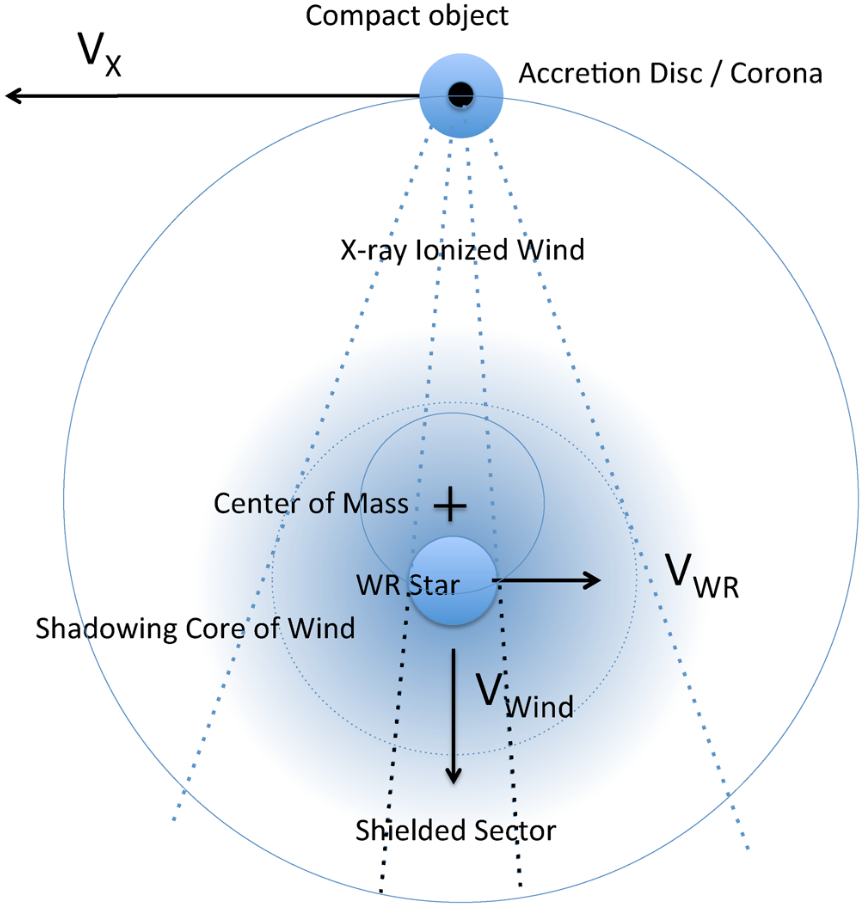
\includegraphics[width=\textwidth]{./images/WRwindIC10X-1.png}
	\end{minipage}
	\hfill
	\begin{minipage}{.60\textwidth}
		\centering
		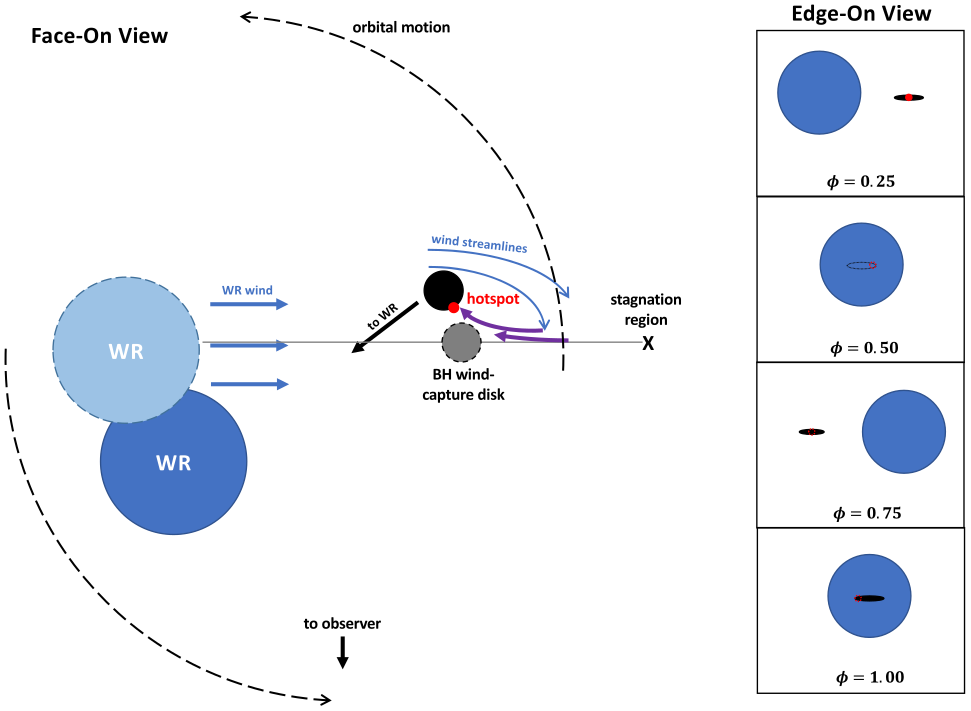
\includegraphics[width=\textwidth]{./images/WRwindNGC300.png}	
	\end{minipage}
	\caption{\emph{Left:} Standard model for the formation of emission lines in WR--BH binaries. Atoms ionized by the X-ray radiation of the compact object accretion disk emit UV/optical/IR lines in the cooler region of the Wolf-Rayet wind: the one shielded by the Wolf-Rayet star itself. The emission has maximum redshift when the Wolf-Rayet star is in superior conjunction ($\phi = 0$), no Doppler shift in quadrature ($\phi = 0.25,0.75$) and maximum blueshift in inferior conjunction ($\phi = 0.5$), as depicted by Laycock et al.\ \cite{ICX10X-1_Laycock2015_revisited}. \emph{Right:} Alternative model for the formation of He II emission lines that could justify the $\Delta \phi = 0.3$ phase offset observed in NGC 300 X-1. The He II lines could form in the extended accretion stream that lags behind the black hole and channels the atoms to the accretion disk, where it forms a hot-spot \cite{NGC300X-1_Binder2021_BHpreciso}.}\label{fig:WRBHwind}
\end{figure}


\paragraph{NGC 300 X-1} NGC 300 X-1 shares many similarities with IC 10 X-1: both have an orbital period of $\sim 30-35$ hours, Wolf-Rayet star mass of $15-35~\msun$ and, most importantly, compact object mass revisited, because the previous determinations with He II emission lines turned out to be unreliable.\\

Crowther et al.\ \cite{NGC300X-1_Crowther2010} characterized the Wolf-Rayet in NGC 300 X-1 from fits to the optical spectra, obtaining luminosity $\log(L_{\rm WR}/\lsun) \sim 5.92$, mass loss rate $\mdot \sim 5 \times 10^{-6}~\msun~\yr^{-1}$, terminal wind velocity $v_{\inf} \sim 1300$ km/s and effective temperature $T_{\rm eff} = 65$ kK. As for IC10 X-1, the authors adopted mass-luminosity relations of Schaerer \& Maeder \cite{schaerer1992MLrelationWR}, finding a best-fit mass of $\mwr = 26_{-5}^{+7}~\msun$. However, since the calibration of the absolute visual magnitude could have been contaminated by nearby sources and altered the fit results, the authors also propose a corrected luminosity of $\log(L_{\rm WR}/\lsun) \sim 5.57$ implying a spectroscopic mass of $\mwr = 15_{-2.5}^{+4}~\msun$. Unlike IC10 X-1, NGC300 X-1 does not exhibit eclipses and geometric arguments indicate an inclination angle of $i=60^{\circ}-75^{\circ}$. Adopting these inclination angles and both Wolf-Rayet mass estimates into the mass function extracted from He II $\lambda=4686$ \AA~line, Crowther et al.\ estimated a black hole mass of $
\mbh \sim 14-23~\msun$.\\

Binder et al.\ \cite{NGC300X-1_Binder2021_BHpreciso} calculated updated X-ray ephemeris and extracted UV spectra that exhibited a strong He II $\lambda=1640$ \AA~ emission line. They combined them with the Doppler shifts of the He II $\lambda=4686$ \AA ~line obtained by Crowther et al.\ \cite{NGC300X-1_Crowther2010}, finding that the resulting radial velocity curve was shifted by $\Delta \phi = 0.3$ with respect to the X-ray light curve: He II lines were not reliable tracers of the orbital motion also in NGC 300 X-1, as Laycock et al.\ \cite{laycock2015_IC10X1_measuredshift} already found in IC10 X-1. Binder et al.\ find that the UV He II $\lambda=1640$ \AA~line luminosity seems to be correlated with the visibility of the accretion disk, being brighter when the disk is observable ($\phi \sim 0-0.25$) and dimmer when the disk is partially hidden by the Wolf-Rayet star ($\phi \sim 0.5$). The correlation seems to support the alternative formation scenario for He II emission lines depicted in the right-hand panel of Fig.\ \ref{fig:WRBHwind}. According to this alternative mechanism, UV and optical He II emission lines are not formed in the shielded region of the Wolf-Rayet wind but, instead, in the shocked regions within the accretion stream and, eventually, in hot spots on the accretion disk. In particular, the accretion streams usually lag behind the black hole and are more extended than the accretion disk, possibly explaining the offset in the He II lines.

In contrast, the weaker C IV $\lambda=1550$ \AA~line provides a radial velocity curve that likely traces the orbital motion of the Wolf-Rayet star, with a phase offset consistent with zero $\Delta \phi = 0.03 \pm 0.03$. Binder et al.\ coupled this radial velocity curve to their precise determination of the orbital period $P=32.7921 \pm 0.0003$ hours to estimate the compact object mass. In particular, they found a mass of $\mbh = 17 \pm 4~\msun$ assuming the best-fit Wolf-Rayet mass of $\mwr = 26_{-5}^{+7}~\msun$ from Crowther et al.\ \cite{NGC300X-1_Crowther2010}. Similarly, the second best-fit value of $\mwr = 15~\msun$ reduced the compact object mass to $\mbh = 13~\msun$. Assuming a black hole mass of $\mbh = 17(12)~\msun$, Binder et al.\ used Kepler's third law to find an orbital separation of $a = 18.2~(15.8)~\rsun$, that, coupled with the corresponding Wolf-Rayet radii of $R_{\rm WR} = 7.2~(4.8)~\rsun$, imply a Roche lobe filling factor of $R_{\rm WR}/R_L = 0.95 (0.77)$: NGC 300 X-1 is unlikely undergoing a RLO and, instead, is a wind-fed system. The estimate on the Wolf-Rayet radii comes from fits with \texttt{PoWR} non-LTE atmospheres \cite{WRnonLTEatmospheresPoWR_Todt2015} to UV spectra, resulting in a WNE classification with higher estimate for the Wolf-Rayet mass loss rate $\mdot \sim 4 \times 10^{-5}~\msun~\yr^{-1}$.



\paragraph{M101 ULX-1} Ultraluminous X-ray sources (ULXs) have luminosity $L_X \gtrsim 10^{39}~\rm erg~s^{-1}$ and are usually interpreted either as an intermediate black hole $M_{\rm IMBH} \gtrsim 100-1000~\msun$ accreting below the Eddington limit (see Sec.\ \ref{eq:Eddingtonaccretion}) or as a neutron star or  stellar mass black hole with ongoing super-Eddington accretion. M101 ULX-1 is classified as ultraluminous X-ray source because it was discovered with a luminosity of $L_X \approx 3 \times 10^{39}~\rm erg~s^{-1}$. \\

In 2013, Liu et al.\ \cite{M101ULX-1_Liu2013} were able to characterize the system components by extracting an optical spectra when the source was in its low state: in fact, similar sources in the high state have optical emission dominated by the accretion disk and cannot be used to detect emission lines from non-degenerate stars. The spectra of Liu et al.\ revealed a large orbital period of $P=8.2$ days and confirmed that the system is composed of a Wolf-Rayet star and a stellar-sized black hole. Fits of non-LTE atmospheres characterized the Wolf-Rayet to be a WN sub-type with luminosity $\log(L_{\rm WR}/\lsun) \sim 5.73$, mass loss rate $\mdot \sim 2 \times 10^{-5}~\msun~\yr^{-1}$, terminal wind velocity $v_{\inf} \sim 1300$ km/s and effective temperature $T_{\rm eff} = 48$ kK. The fit estimated also a mass of $\mwr = 17.5~\msun$, in agreement with the $\mwr = 19~\msun$ mass obtained adopting the mass-luminosity relations of Schaerer \& Maeder \cite{schaerer1992MLrelationWR}.

Liu et al.\ used the strong He II $\lambda=4686$ \AA ~line to extract the radial velocity curve and found a lower limit for the compact object mass: $M_{\rm BH, min} \sim 4.5~\msun$ for an edge-on system. While this result provides dynamical evidence for a black hole, the orbital inclination is not constrained and does not allow more detailed estimations of its mass. Therefore, similarly to the procedure used by Koljonen et al.\ \cite{CygX-3_Koljonen2017} for Cyg X-3 and explained in Sec.\ \ref{subsec:cygx3observations}, Liu et al.\ estimated the mass of the black hole imposing that it is sufficient to produce the observed accretion luminosity $L_X \sim 3 \times 10^{38}~\rm erg~s^{-1}$. Different accretion efficiencies $\eta$ and different black hole rotational velocities result in different minimum black hole masses. Therefore the authors considered two extreme cases: a Schwarzschild black hole with low accretion efficiency $\eta = 0.06$, or  a maximally spinning Kerr black hole with $\eta = 0.42$. Liu et al.\ found that in the first case a minimum mass of $\sim 42~\msun$ is required while, in the latter case, a much lower minimum mass of $\sim 8~\msun$ is sufficient to match the luminosity. Overall, the black hole seems to be $M_{\rm BH, min} \gtrsim 8-42~\msun$. 

The authors further argue that a black hole in the $\sim 20-30~\msun$ range should be more probable, but they base their reasoning on the comparison with the masses of IC 10 X-1 and NGC 300 X-1 black holes, at that time not yet revised for the errors introduced by the He II - derived velocity curve (as discussed in the previous paragraphs and in \cite{ICX10X-1_Laycock2015_revisited,NGC300X-1_Binder2021_BHpreciso}). Therefore, in Tab.\ \ref{tab:observations} I reported the minimum black hole masses to provide an order-of-magnitude estimate.



\subsection{CXOU J123030.3+413853, CXOU J004732.0-251722.1 and CG X-1}\label{subsec:uncertainWRcandidates}

\paragraph{Three uncertain candidates} CXOU J123030.3+413853, CXOU J004732.0-251722.1 and CG X-1 are WR--BH candidates only from the analysis of their X-ray variability: no UV, optical or IR spectrum are yet available \cite{observations}. All three sources have peak luminosity of $L_X \sim 10^{38}-10^{40}~\rm erg~s^{-1}$ that allows them to be classified as ULXs. 

The period of the X-ray light curves is assumed to be the orbital period as is the one reported in Tab.\ \ref{tab:observations}, although there is no independent evidence that this assumption is correct. The three candidates belong to three starburst galaxies with star formation rates of $\sim 2-4~\msun~\yr^{-1}$, supporting the possibility that they are at least HMXBs \cite{observationsZSFR_Mapelli2010a}.

\paragraph{Evidences for WR--BH binaries} The WR--BH classification is based on the detection of slow rises and fast decays in the X-ray light curve. Similar modulations are present also in the light curve of Cyg X-3 and are usually interpreted as regions of stronger and lighter interaction between the ionized matter of the Wolf-Rayet winds and the X-radiation produced by the accretion disk, respectively \cite{observations}. Moreover, the elevated X-ray luminosity of the three candidates supports a black hole compact object, given that a neutron star should, instead, accrete above the Eddington limit (see Sec.\ \ref{eq:Eddingtonaccretion}).









\chapter{Models and simulations with \texttt{SEVN}}
\paragraph{Chapter outline} In this chapter I will describe the population-synthesis code \texttt{SEVN} adopted in this thesis, discussing its most relevant options and modules with particular attention to the models of core-collapse supernova and kicks explored in this work. I will then explore the assumptions, initial conditions and parameters adopted to simulate 24 representative populations of binaries, each containing $10^6$ systems.


\section{\texttt{SEVN}: a population-synthesis code}\label{sec:SEVN}
\subsection{Code properties}\label{subsec:SEVNproperties}
\paragraph{The code} \texttt{SEVN} (acronym for \emph{Stellar EVolution for N-body simulations}) is a population-synthesis code written in \texttt{C++} able to calculate the evolution of a large number of single stars or binary systems in a short amount of time ($\sim 10^{6}$ binary systems are evolved in $\sim 12$ hours) \cite{spera2019_mergingBBH}. Like other population-synthesis codes available in the literature, \texttt{SEVN} can be used to simulate a population of stellar objects and understand their properties.

\paragraph{A fast tool for simulations} Properly evolving two stars in a binary system is computationally expensive because it would require to solve on-the-fly the system of differential equations determining the stellar structure. Similar calculations can be carried out by the \texttt{MESA} stellar evolution code, but allow to simulate only $\lesssim 5$ systems per day on a single CPU \cite{MESA2015BinaryMT}. In contrast, population-synthesis codes evolve the stars by means of pre-computed fitting formulas or evolutionary tables. This approach, coupled with analytic and semi-analytic prescriptions for binary evolution and with an adaptive time-step scheme, allows to speed up the calculations, at the expense of physical accuracy. The possibility to rapidly simulate a large number of systems is crucial to study the  demography of LVC binary black holes: only $\lesssim 0.01$ \% of a statistically motivated initial binary population merges via gravitational wave emission within a Hubble time \cite{spera2019_mergingBBH}.

\paragraph{Stellar evolution with interpolation tables} Many population-synthesis codes, like \texttt{MOBSE} \cite{giacobbomapelli2018_mobse_fryer}, \texttt{STARTRACK} \cite{Belczynski2010_WRwindsSTARTRACK} and \texttt{COSMIC} \cite{breivik2020cosmicpopsynth}, implement stellar evolution through updates to \texttt{BSE} fitting formulas \cite{hurley2000}. These fits are based on stellar evolution tracks computed in 1998 by Pols et al.\ \cite{Pols1998evotracks}, even though our knowledge of massive star evolution has changed significantly since 1998 \cite{marchant2021_masstransferMESA,klencki2021CE}. In addition, these fitting formulas are extremely difficult to update in order to match new evolutionary tracks. 

In contrast, \texttt{SEVN} does not use fitting formulas but evolves the stars interpolating a set of pre-computed evolutionary tracks: this approach makes \texttt{SEVN} more flexible and easier to update with the latest stellar evolution results.

\paragraph{The \texttt{PARSEC} tables} Currently, \texttt{SEVN} implements evolutionary tables calculated with \texttt{MESA} (also known as \texttt{MIST} isochrones \cite{MIST_Choi2016}) and with \texttt{PARSEC} \cite{parsec2015_chen, MassGapStellarEvo_Costa2021}.  The default tables and the ones used in this thesis are the \texttt{PARSEC} ones, calibrated for massive stars and calculated with a grid of models spanning $2.2~\msun \leq \mzams \leq 350~\msun$ and $0.0001 \leq \zzams \leq 0.04$. I used these tracks to generate the Hertzsprung-Russell diagrams in Fig.\ \ref{fig:HRdiagrams}. Stellar winds prescriptions for massive stars described in Sec.\ \ref{subsec:stellarwinds} were implemented according to the input physics assumptions discussed in Sec.\ \ref{subsec:stellarevo} \cite{parsec2015_chen,MassGapStellarEvo_Costa2021}. 

\paragraph{Interpolation method} As explained in Sec.\ \ref{subsec:stellarevo}, stellar properties are determined mainly by mass and metallicity, thus, each evolutionary track can be identified with the values at the ZAMS ($\mzams,\zzams$). It is possible to represent different stellar track in a three-dimensional space ($M,Z,t$) like the one depicted in Fig.\ \ref{fig:SEVNinterpolation}: at each time $t$, a point in the ($M,Z$) plane represents a star with a one-to-one association with its other properties (luminosity, effective temperature, etc.).

The \texttt{PARSEC} tracks are not calculated for every possible combination of stellar parameters but only for representative ones, providing a reference grid in the ($M,Z$) plane for each evolutionary stage. If, as it often happens, \texttt{SEVN} needs to evolve a star with intermediate properties with respect to the provided tracks, the code will interpolate the star by means of weighted average of the closest four tracks in the ($M,Z$) plane. For instance, to evolve a $\mzams = 33~\msun$ star at $\zzams=0.015$ metallicity, not directly generated by \texttt{PARSEC}, \texttt{SEVN} will interpolate its initial properties from the closest available \texttt{PARSEC} tracks: $\mzams = 32~\msun$ and $\mzams = 34~\msun$ at $\zzams = 0.014$ and $\zzams = 0.017$.


\begin{figure}
	\centering
	\def\svgwidth{0.5\textwidth}
	\import{./images/}{interpolation.pdf_tex} 
	\caption{Schematic representation of star interpolation carried out by \texttt{SEVN}. Original four evolutionary tracks obtained from a stellar evolution code, like \texttt{PARSEC} or \texttt{MESA}, are represented by the four coloured circles. For didactic purposes, stars on the top (cyan and black circles) are assumed to be more massive and to lose mass more rapidly than stars on the bottom (blue and pink circles), with the more metallic one (black circle) losing even more mass. \texttt{SEVN} interpolates a star with desired initial masses and metallicity ($M(t_1),Z(t_1)$) falling within the depicted region by weighting the properties of the four closest tracks, as explained in Sec.\ \ref{subsec:SEVNproperties}. The weighted interpolation is repeated at each evolutionary time-step $t_i$. I created the scheme following the description provided in Iorio et al.\ in preparation.}\label{fig:SEVNinterpolation}
\end{figure}






\subsection{Stellar phases}\label{subsec:stellarphasesSEVN}
\paragraph{Macro phase $\boldsymbol{p}$:} \texttt{SEVN} identifies three macro-phases $p$ to indicate that a star already formed a H, He or CO core \cite{spera2019_mergingBBH}. The macro-phase division is used as a proxy for the internal structure of the star, allowing to match the same structure in the interpolating tracks. In fact, at each evolutionary time it is possible to calculate the percentage of macro-phase time already elapsed and select only interpolating tracks at the same evolutionary stage (e.g., at 10\% of the He phase). A match in the lifetime percentage is required also when \texttt{SEVN} needs to change the interpolating tracks, for instance because the star becomes a Wolf-Rayet or loses mass after a mass transfer episode. 

\paragraph{\texttt{BSE} phases:} \texttt{SEVN} implements many classifications to account for the stellar properties, burning stages and binary processes, as explained in more detail in Iorio et al.\ in preparation. Here, I will discuss only the classification presented by Hurley et.\ al \cite{Hurley2002}, since \texttt{SEVN} implements the main binary evolution processes as described in the aforementioned paper, with some minor changes (see next section Sec.\ \ref{subsec:masstransferSEVN}). 

I will limit the discussion to the phases reported in Tab.\ \ref{tab:phasesqcritSEVN}, that are the only phases regarding evolution and mass transfer of the massive stars considered in this thesis (for instance, I will neglect white dwarfs). Moreover, \texttt{BSE} phases 6 and 9 reported in the previous version of \texttt{SEVN} \cite{spera2019_mergingBBH} are re-absorbed in, respectively, phases 5 and 8 in the updated version of \texttt{SEVN} that I used in this thesis and that is discussed in Iorio et al.\ in preparation.\\ 
\\

Stars are classified as main sequence (\texttt{BSE} phase = 1) only if their initial mass is $\mzams \geq 0.7~\msun$, sufficient to have a radiation-dominated envelope. During the following H-shell burning phase, the hydrogen envelope expands and eventually becomes fully convective (see Sec.\ \ref{subsec:stellarevo} for more details). Considering the mass fraction of the convective over the total envelope mass $f_{\rm conv}= M_{\rm conv}/M_{\rm env}$, the \texttt{BSE} classification distinguishes Hertzsprung-gap stars ($f_{\rm conv} < 0.33$, \texttt{BSE} phase = 2) from first giant branch stars ($f_{\rm conv} \geq 0.33$, \texttt{BSE} phase = 3).  Once He-burning starts, the convective envelope fraction further discriminates between stars burning He in their cores ($f_{\rm conv} < 0.33$, \texttt{BSE} phase = 4) or in shells ($f_{\rm conv} \geq 0.33$, \texttt{BSE} phase = 5).

The \texttt{BSE} classification is based on the stellar evolution tracks of Pols et al.\ \cite{Pols1998evotracks}, where the difference between the two classes was more evident than in the massive stars considered here. For instance, in the HR diagrams shown in Fig.\ \ref{fig:HRdiagrams}, the start of the H-shell burning phase is in reality depicted with \texttt{BSE} phase = 3, since the marker was almost coincident with the, not shown, marker for \texttt{BSE} phase = 2: the evolution is so fast that the envelope becomes rapidly convective. \\

Once a star ignites central helium, \texttt{SEVN} checks whether the helium mass fraction is larger than 97.9\% of the total mass of the star: if that is the case, the star becomes a Wolf-Rayet. As already explained in Sec.\ \ref{subsec:stellarevo}, \texttt{SEVN} evolves Wolf-Rayet stars with pure-He stars, interpolating them from a dedicated set of tables. Pure-He stars, similarly to ``normal'' H-rich stars, evolve through an equivalent main sequence and Hertzsprung-gap phase characterized by helium burning in the core and in the shell, respectively. A pure-helium star at the beginning of its main sequence is obtained artificially removing the hydrogen envelope to a ``normal'' star in the moment it starts the core-He burning. The resulting \emph{pure-He ZAMS} star is then evolved with standard stellar evolution prescriptions and provides one of the interpolating tracks in the pure-He tables.\\

I remind that, as discussed in Sec.\ \ref{subsec:stellarevo}, in this thesis I will overcome the \texttt{BSE} phase classification and consider as Wolf-Rayet stars also the ones that are not yet pure-helium (representative of WC and WO sub-types) but are still able to retain an external hydrogen layer, with superficial hydrogen abundance $H_{\rm sup} \geq 0.3$ (representative of WNL and WNE sub-types). I will be able to carry on this more physically-motivated and detailed analysis only because I will use \texttt{PARSEC} tables: unlike other interpolation tables, the \texttt{PARSEC} ones provide superficial abundances.



\begin{table}
    \centering
    \begin{tabular}{llllcc}
        \toprule
        Stellar phase & Burning & $p$ & Condition & \texttt{BSE} phase &  $q_{\rm crit}$ \\ 
        \midrule
        Main sequence           & H-core    &  H   & $\mzams \geq 0.7~\msun$          &  1  & 3.0        \\
        Hertzsprung-gap         & H-shell   &  He  & $f_{\rm conv} < 0.33$       &  2  & 4.0        \\
        First giant branch      & H-shell   &  He  & $f_{\rm conv} \geq 0.33$    &  3  & Equation \ref{eq:qcritgiants} \\
        Core He burning         & He-core   &  He  & $f_{\rm conv} < 0.33$       &  4  & 3.0 \\ 
        Asymptotic giant branch & He-shell  &  CO  & $f_{\rm conv} \geq 0.33$    &  5  & Equation \ref{eq:qcritgiants} \\
        \hline
        Wolf-Rayet              & He-core   &  He  & $M_{\rm He} > 0.979~M$  &  7  & 3.0 \\ 
        Wolf-Rayet              & He-shell  &  CO  & $M_{\rm He} > 0.979~M$  &  8  & 0.784 \\ 
        \bottomrule
        \end{tabular}
    \caption{Stellar evolution phases with their equivalent nuclear burning and \texttt{SEVN} macro-phase $p$ used for interpolation (Sec.\ \ref{subsec:SEVNproperties}). Stars are also classified with their equivalent \texttt{BSE} phase \cite{Hurley2002}, imposing a condition on the fraction of convective envelope with respect to the total envelope mass $f_{\rm conv}= M_{\rm conv}/M_{\rm env}$ or on the total helium mass fraction $M_{\rm He}/M$. For each \texttt{BSE} phase of the donor star, \texttt{SEVN} associates a critical donor-to-accretor mass ratio $q_{\rm crit}$ that, if overcome, triggers a Roche lobe overflow unstable on the dynamical timescale.}\label{tab:phasesqcritSEVN}
\end{table}



\subsection{Mass transfer}\label{subsec:masstransferSEVN}
\paragraph{Roche lobe overflow stability criterion} As anticipated in Sec.\ \ref{subsec:Rochelobeoverflow}, Roche lobe overflow stability depends on the donor-to-accretor mass ratio $q=M_{\rm d}/M_{\rm a}$ and helium core prominence in the donor star $M_{\rm He,d}/M_{\rm d}$. Following \texttt{BSE} prescriptions suggested by Hurley et al.\ \cite{Hurley2002}, \texttt{SEVN} triggers a Roche lobe overflow unstable on the dynamical timescale whenever the binary mass ratio is larger than a critical value $q_{\rm crit}$, function of the core mass ratio

\begin{equation}
    q \geq q_{\rm crit}(M_{\rm He,d}/M_{\rm d})
\end{equation}

The adopted $q_{\rm crit}$ values, reported in Tab.\ \ref{tab:phasesqcritSEVN}, were calculated with fits to stellar models produced in 1998 by Pols et al.\ \cite{Pols1998evotracks}, except for models on the giant branch (\texttt{BSE} phase = 3) and asymptotic giant branch (\texttt{BSE} phase = 5), whose $q_{\rm crit}$ 

\begin{equation}\label{eq:qcritgiants}
   q_\mathrm{crit} = 0.362 + \frac{1}{3\left(1-\frac{M_\mathrm{He,d}}{M_\mathrm{d}}\right)}.
\end{equation}

are calibrated on the  models of condensed polytropes by Hjellming \& Webbink \cite{hjellmingwebbink1987_coreRLOF}, as already discussed in Sec.\ \ref{subsec:Rochelobeoverflow}.


\paragraph{Stable Roche lobe overflow} If $q < q_{\rm crit}$, \texttt{SEVN} triggers a Roche lobe overflow that is stable on the dynamical timescale. Since the donor star retains only the mass within its Roche lobe radius $R_{\rm L,d}$, stellar winds and tides in this phase are calculated adopting $R_{\rm L,d}$ as an equivalent stellar radius. The real donor stellar radius $R_{\rm d}$ is, instead, only used to calculate the mass loss rate with an updated version of the prescriptions of Hurley et al.\ \cite{Hurley2002}

\begin{equation}\label{eq:masslossrateRLSEVN}
\mdot_{\rm d, nuc} = F(M_\mathrm{d}) \left( \ln \frac{R_\mathrm{d}}{R_\mathrm{L,d}} \right)^3~\msun~\yr^{-1} 
\end{equation}


where the normalization factor $F(M_\mathrm{d})$ for the massive donors considered in this thesis is calibrated to allow stable mass-transfer (see Iorio et al.\ in preparation) and is given by

\begin{equation*}
F(M_\mathrm{d}) =  3 \times 10^{-6} \left[ \min \left( M_\mathrm{d}, 5.0 \right) \right]^2 \times
\begin{cases}
\max \left( \frac{M_\mathrm{d, env}}{M_\mathrm{d}} ,0.01 \right) & \texttt{BSE} ~\text{phase = 2} \\
1 & \text{others}
\end{cases}
\end{equation*}

Eq.\ \ref{eq:masslossrateRLSEVN} indicates mass loss rates for Roche lobe overflows stable on the nuclear timescale. However, as already discussed in Sec.\ \ref{subsec:Rochelobeoverflow}, stars losing their external envelopes may exit their thermal equilibrium, undergoing a Roche lobe overflow stable on the dynamical timescale but unstable on the thermal one. If this is the case, the mass loss rate expected by Eq.\ \ref{eq:masslossrateRLSEVN} cannot exceed the order-of-magnitude mass loss rate caused by the star instability

\begin{equation}
    \mdot_{\rm d, nuc} \leq \mdot_{\rm d, max}
\end{equation}

Depending on the stellar type, the maximum mass-loss rate is estimated with a dynamical or thermal timescale following Hurley et al.\ \cite{Hurley2002} prescriptions. In particular, giant stars with a core-envelope separation will be thermal-limited while main sequence stars and Wolf-Rayet stars that did not yet developed a CO core will be dynamical-limited

\begin{equation}
    \mdot_{\rm d, max} = 
    \begin{cases}
        \mdot_{\rm d, KH} = \frac{M_{\rm d}}{\tau_{\rm d, KH}}   & \qquad \texttt{BSE} ~\text{phase = 2,3,4,5,8} \\
        \mdot_{\rm d, dyn} = \frac{M_{\rm d}}{\tau_{\rm d, dyn}} & \qquad \texttt{BSE}~\text{phase = 1,7}
    \end{cases}
\end{equation}

The respective timescales are calculated as function of the donor envelope mass $M_{\rm env}$ and total mass $M$, radius $R$ and luminosity $L$

\begin{equation}
    \tau_{\rm KH} = 10^7 ~\frac{M M_{\rm env}}{RL}~\yr \qquad \qquad \tau_{\rm dyn} = 5.05 \times 10^{-5}~ \sqrt{\frac{R^3}{M}}~\yr
\end{equation}

Once the donor mass loss rate is established $\mdot_{\rm d}$, the mass accreted by the companion $\mdot_{\rm a}$ is calculated as a fixed fraction $f_{\rm MT}$ of it

\begin{equation}\label{eq:accretionrateSEVN}
    \mdot_{\rm a} = f_{\rm MT} \mdot_{\rm d} \qquad \qquad f_{\rm MT} \in [0,1]
\end{equation}

The fiducial accreted fraction is $f_{\rm MT} = 0.5$ and is the value adopted in this thesis. The accretion rate calculated with Eq.\ \ref{eq:accretionrateSEVN} is limited by the Eddington one for accreting compact objects, like neutron stars and black holes\footnote{Eddington limited accretion is imposed also for compact objects that are member of a wind-fed system, where accretion is calculated with Eq.\ \ref{eq:windfedaccretion}.}. Moreover, \texttt{SEVN} does not accrete mass onto Wolf-Rayet stars because their winds are assumed to be so strong to rapidly remove any additional layer deposited on their surfaces (see Iorio et al.\ in preparation).




\paragraph{Common envelope} Usually binaries enter a common envelope evolution if there is an over-contact binary, a collision at periastron or the donor undergoes an unstable Roche lobe overflow (see Sec.\ \ref{subsec:Commonenvelope}). However, unlike the previous version of \texttt{SEVN} \cite{spera2019_mergingBBH} and many \texttt{BSE}-derived codes, the \texttt{SEVN} version adopted in this thesis does not form over-contact binaries with both stars filling their Roche lobe simultaneously because, as explained in the previous paragraph, the Roche lobe overflow routine considers the Roche lobe radius as an equivalent stellar radius. A similar assumption is necessary to explain the neutron stars merger rates: without it, too many systems would enter a common envelope evolution and merge prematurely (see Iorio et al.\ in preparation). For the same reason, in this thesis I allowed for collisions only outside the Roche lobe overflow. Apart from this, \texttt{SEVN} routines for common envelope used the standard assumptions and adopt the $\alpha \lambda$ formalism of Webbink et al.\ \cite{Webbink1984_CE}. \\

Following \texttt{BSE} \cite{Hurley2002}, \texttt{SEVN} merges donor stars that enter a dynamically unstable Roche lobe overflow without a well-defined core-envelope separation: it is the case of main sequence and Wolf-Rayet stars that did not yet developed a CO core (\texttt{BSE} phase = 1,7). In contrast, donors with a core (\texttt{BSE} phase = 3,4,5,8) enter the routine for the common envelope evolution: with the right orbital separation the stars could survive in a tighter orbit (see Sec.\ \ref{subsec:Commonenvelope}).

Stars in the Hertzsprung-gap phase (\texttt{BSE} phase = 2) are developing a He core but it is not yet clear if the core-envelope gradient is sufficiently large to allow core survival and envelope ejection in case of a common envelope. Therefore, \texttt{SEVN} implements two possible scenarios: an \emph{optimistic} one where the Hertzsprung-gap star could enter and survive the common envelope and a \emph{pessimistic} one where the star  merges whenever mass transfer becomes dynamically unstable. \\

When a merger occurs, either because both stars still overfill their Roche lobe in the final configuration or because the donor star lacks a well-developed core, the resulting star has final core given by the sum of the two original cores $M_{\rm core,merger} = M_{\rm core, d} + M_{\rm core, a}$. Moreover, since the system was not able to eject the common envelope, \texttt{SEVN} assumes that all the mass is retained, thus the merger product has final mass given by the sum of the original masses $M_{\rm merger} = M_{\rm d} + M_{\rm a}$.





\subsection{Core-collapse supernovae}\label{subsec:SNmodels}
\texttt{SEVN} carries on stellar evolution only up to the end of the CO burning, using the CO core mass to calculate the fate and mass of the compact object produced after a core-collapse supernova (CCSN). Therefore, the end of the CO phase will be hereafter denoted improperly as \emph{pre-SN} phase and will be used to calculate values that should be calculated at the onset of the collapse, like the compactness in Eq.\ \ref{eq:compactness}. Among the CCSN models implemented in \texttt{SEVN}, I will here discuss the three adopted in this thesis, indicated as \emph{rapid}, \emph{delayed} and \emph{compactness}.

\paragraph{Rapid and delayed} \emph{Rapid} and \emph{delayed} models are based on calculations carried out by Fryer et al.\ \cite{Fryer2012}. They used pre-computed fitting formulas to estimate the final CO and FeNi core of pre-SN stars and computed the corresponding compact object masses with the \texttt{STARTRACK} \cite{Belczynski2010_WRwindsSTARTRACK} population-synthesis code, adopting two explosion models. Recalling that in CCSNe the external layers collapse to the proto-compact object, bounce back and then expand again in a neutrino-driven explosion, Fryer et al.\ distinguished between \emph{rapid} and \emph{delayed} explosions for shocks revived, respectively, before and after $\sim 250$ milliseconds from the collapse. 


As shown in the left-hand panels of Fig.\ \ref{fig:remnants}, the more delayed is the explosion and the more difficult is to eject the collapsing mass, favouring the formation of heavier compact objects. The aforementioned figures also highlight a piece-wise trend of the mass of the compact object as a function of the ZAMS mass, especially for the \emph{rapid} model: for instance, stars with $\mzams \sim 23-25~\msun$ form compact objects $\gtrsim 10~\msun$ heavier than stars with similar initial masses ($\mzams \sim 20~\msun$ or $\mzams \sim 26~\msun$). Abrupt jumps in the compact remnant mass reflects its strong sensitivity on the CO core mass. In fact, the baryonic compact object masses $M_{\rm rem, bar}=M_{\rm proto} + M_{\rm fb} $ are calculated as the sum of the proto-compact object mass $M_{\rm proto}$ and the fallback mass $M_{\rm fb}$, both dependent on the CO mass but through different combinations (see Fryer et al.\ \cite{Fryer2012} for the set of equations). The complicated dependence on the CO core mass is removed for $M_{\rm CO} \geq 11~\msun$, where Fryer et al.\ assume that all the mass falls back, causing the baryonic compact remnant mass to be simply the pre-SN mass $M_{\rm rem, bar} = M_{\rm pre-SN}$. As shown in the right-hand panel of Fig.\ \ref{fig:masslostWR}, at solar metallicity only stars with $\mzams \gtrsim 40~\msun$, have $M_{\rm CO} \gtrsim 11~\msun$: stars with lower initial mass have a limited CO growth because of the strong stellar winds (see Sec.\ \ref{subsec:stellarevo} for more details). So far, the methodology to calculate the baryonic compact remnant mass according to the \emph{rapid} and \emph{delayed} model can be schematized as 

\begin{equation}\label{eq:fryermass}
    M_{\rm rem, bar} = 
    \begin{cases}
    M_{\rm pre-SN} & M_{\rm CO} \geq 11~\msun \\
    M_{\rm proto}(M_{\rm CO}) + M_{\rm fb}(M_{\rm CO}) & M_{\rm CO} < 11~\msun 
    \end{cases}
\end{equation}

Recently, Zevin et al.\ \cite{Zevin2020_neutrinolosses} corrected a typo in the prescriptions adopted by Fryer et al.\ \cite{Fryer2012} to account for neutrino losses, finding that they carry away 10 \% of the iron core mass (not 10 \% of the total baryonic mass, as was incorrectly reported by Fryer et al.\ ). Thus, accounting also for the baryonic-to-gravitational mass conversion, \texttt{SEVN} calculates the final gravitational compact remnant mass $M_{\rm rem}$ as in Iorio et al.\ in preparation

\begin{equation}\label{eq:neutrinolosses}
    M_\mathrm{rem} = \max \left\{ \frac{\sqrt{1 + 0.3\,~M_\mathrm{rem, bar}} -1 }{0.15}, M_\mathrm{rem,bar}-0.5~\msun\right\}
\end{equation}




\begin{figure}[t!]
	\begin{minipage}{.60\textwidth}
		\centering
		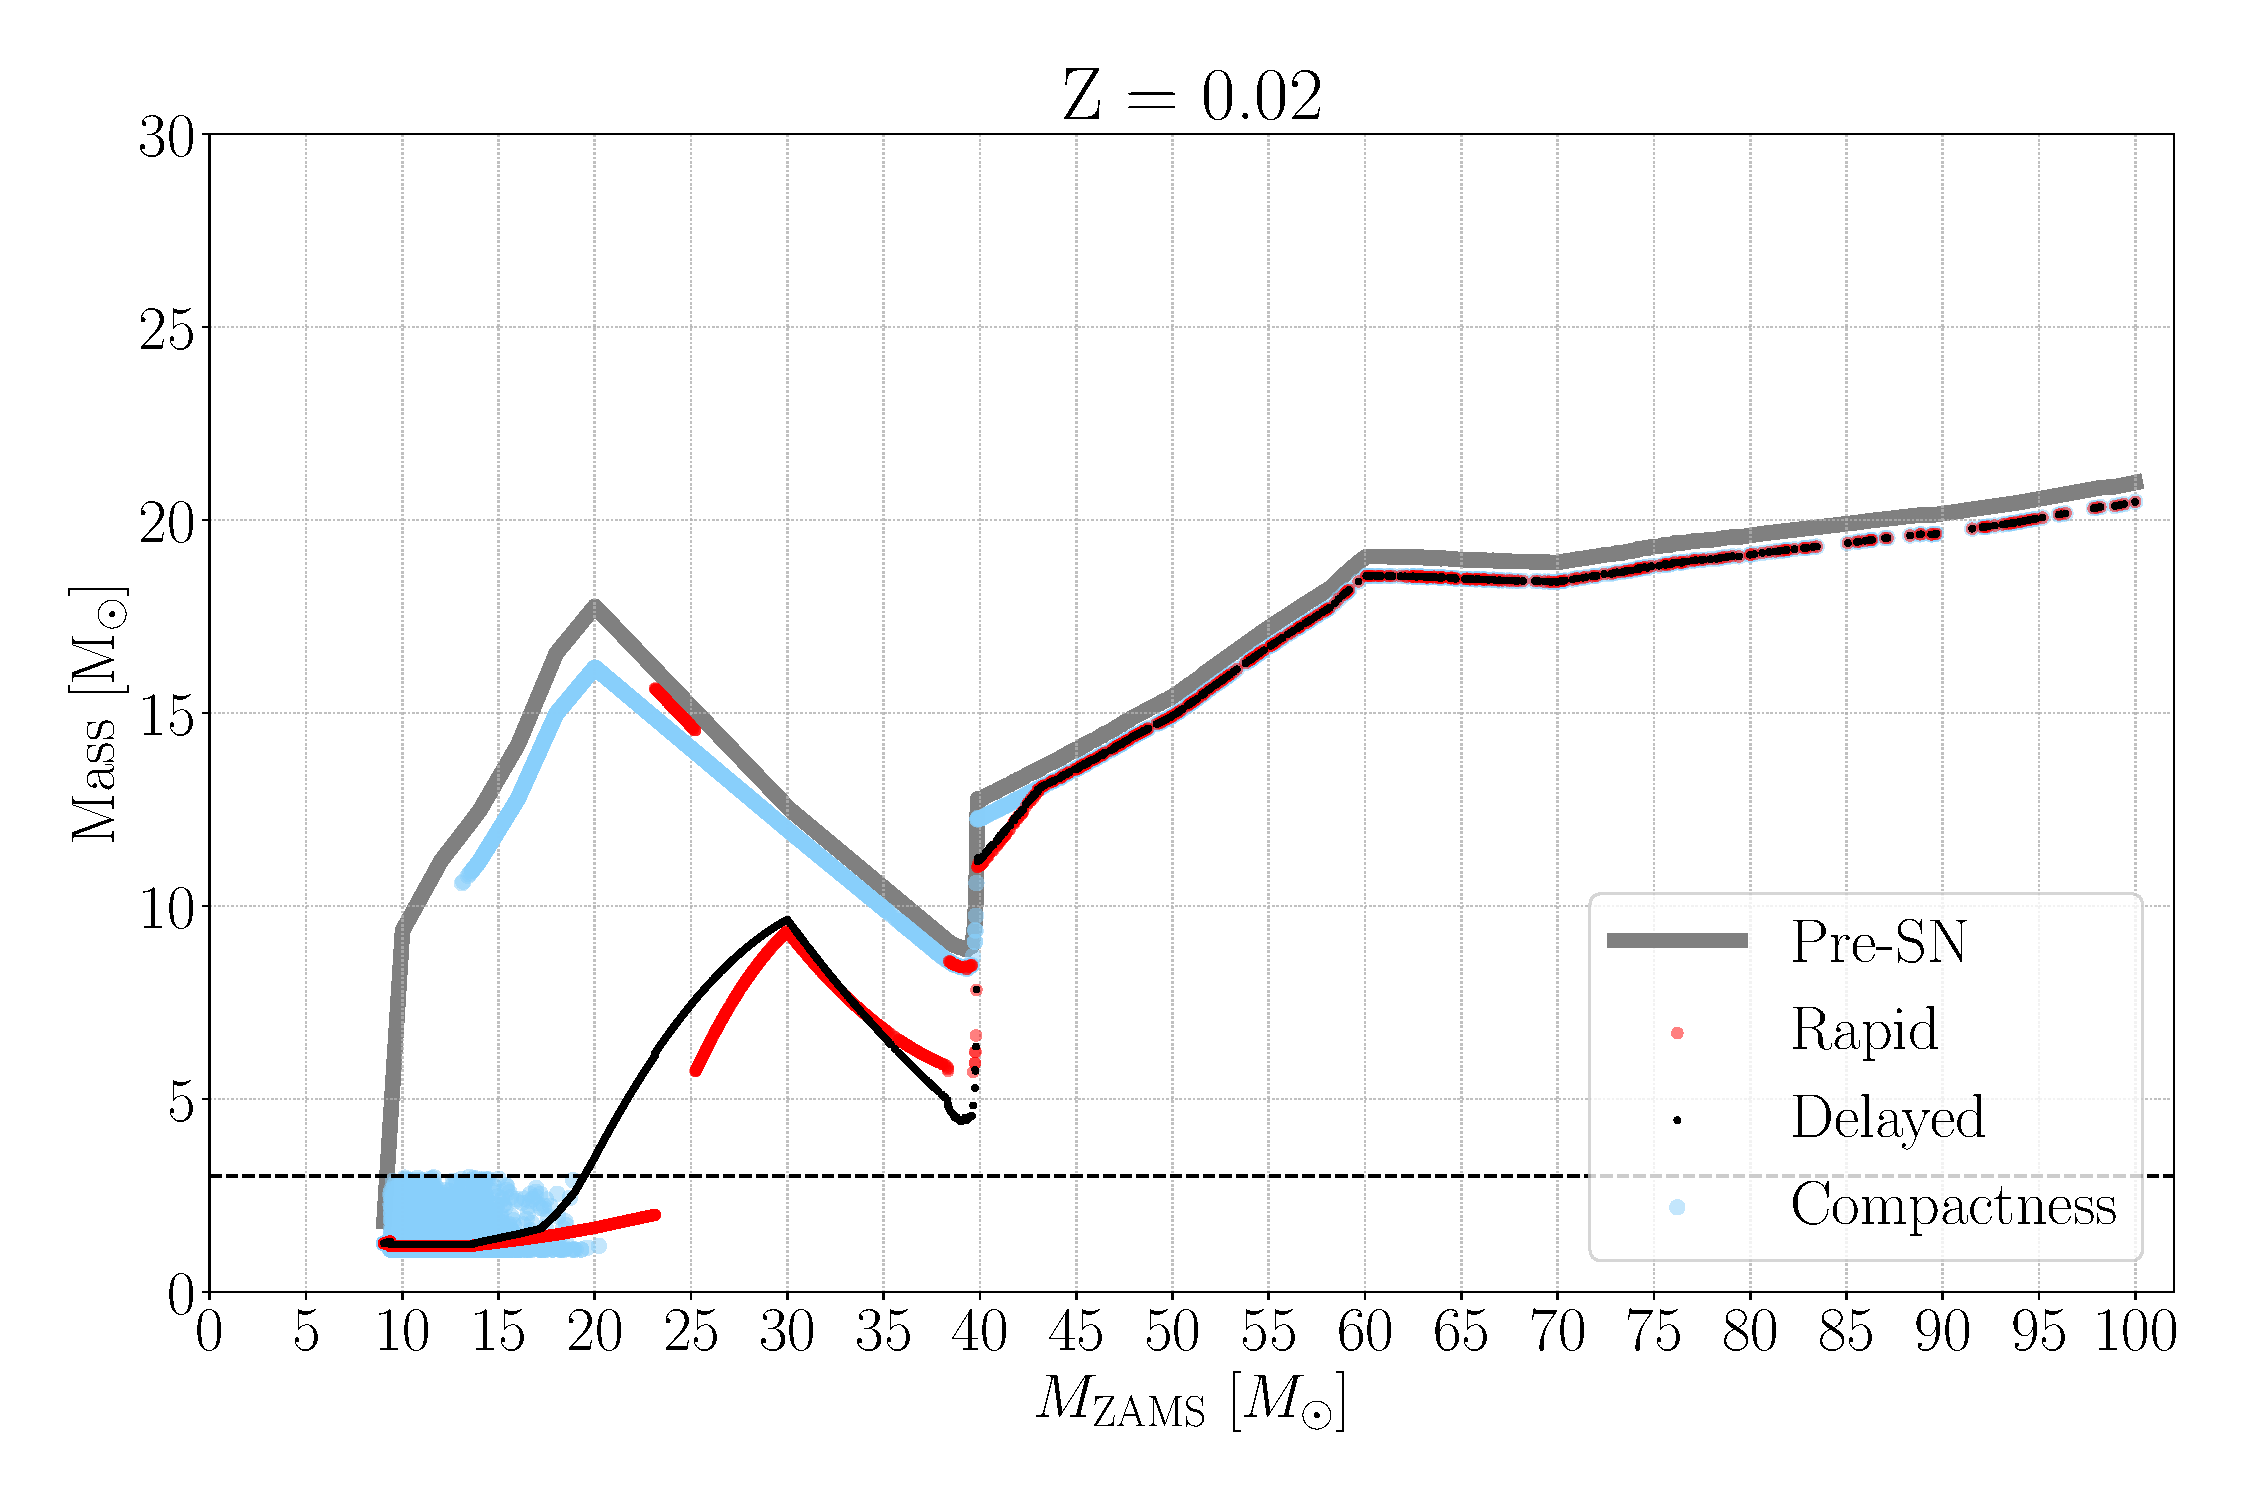
\includegraphics[width=1.05\textwidth]{./images/remnants_Z02.pdf}
	\end{minipage}
	\hfill
	\begin{minipage}{.39\textwidth}
		\centering
		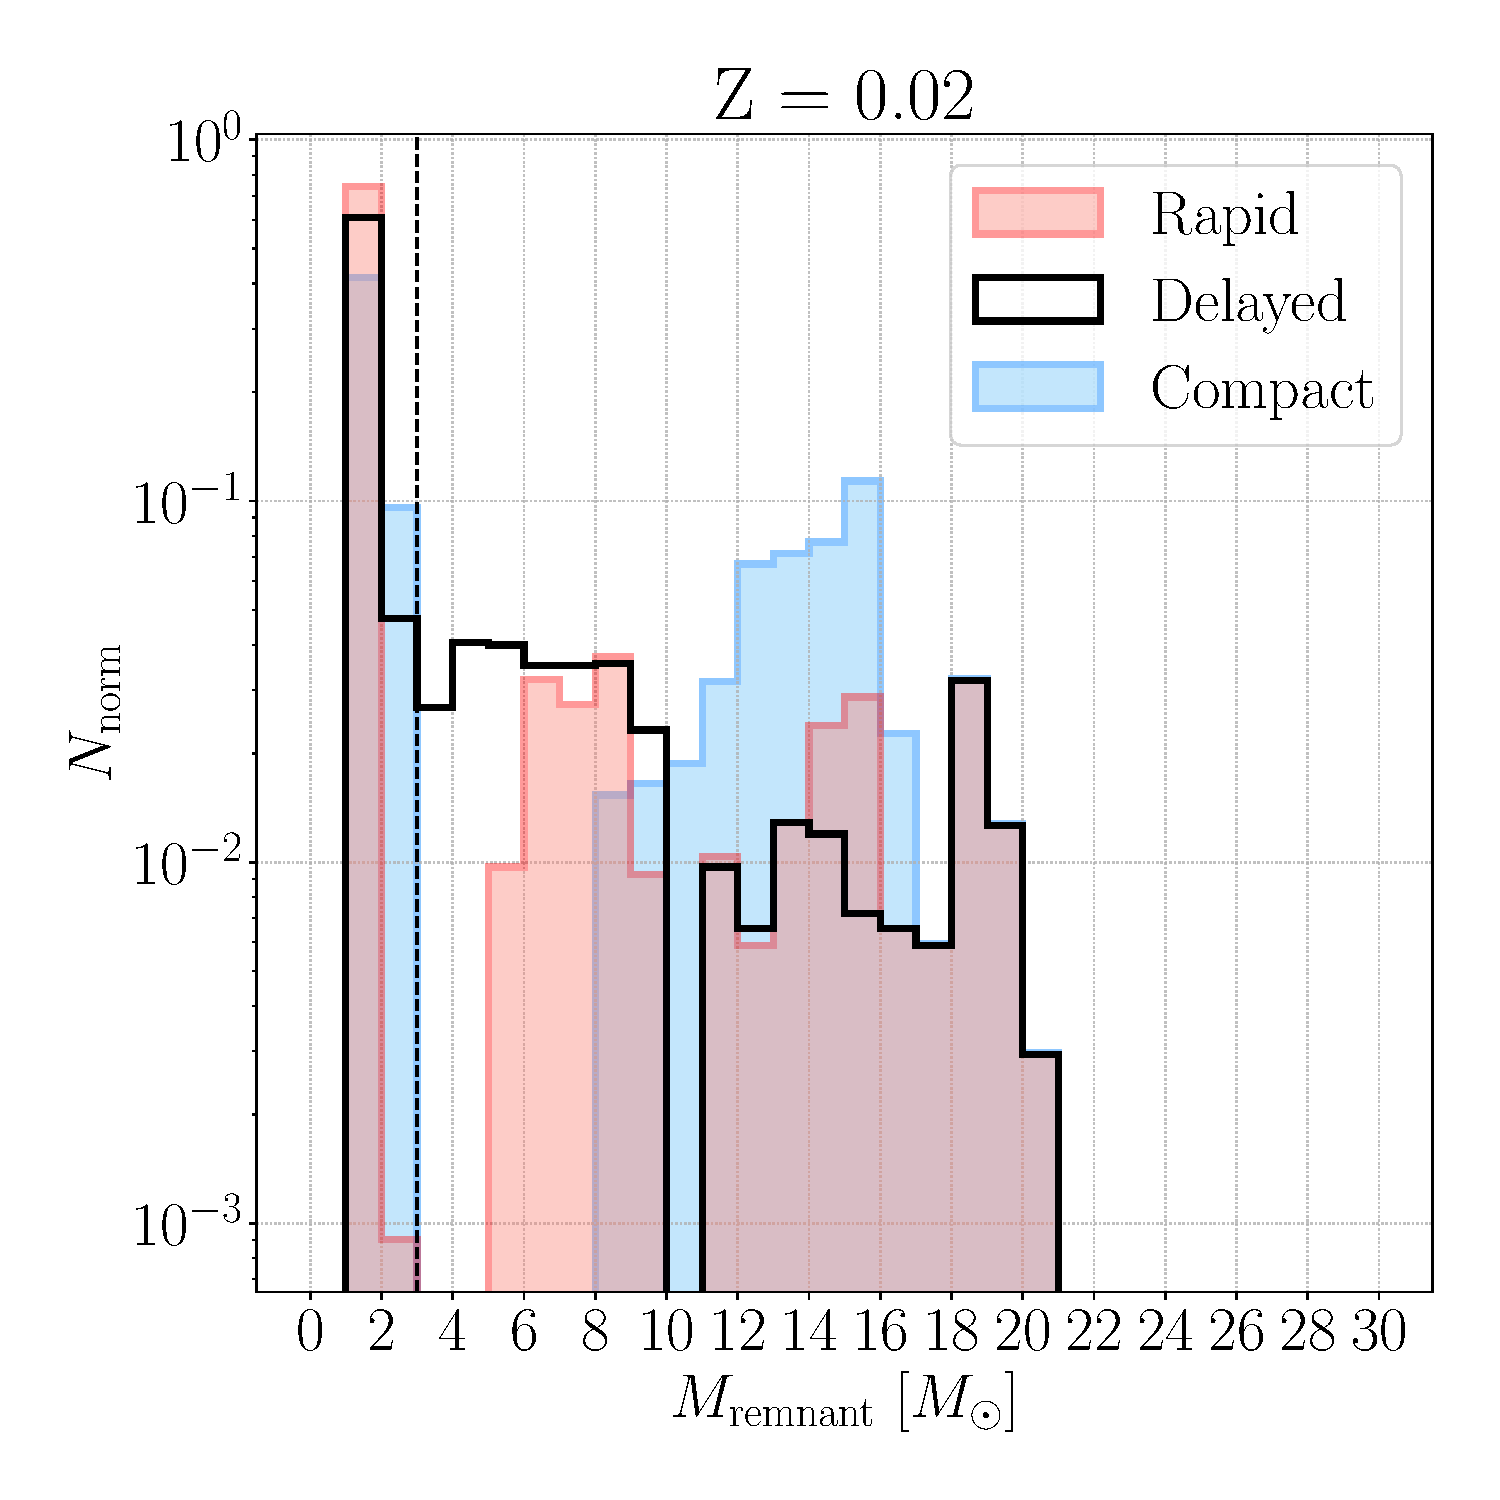
\includegraphics[width=1.05\textwidth]{./images/hist_Z02.pdf}	
	\end{minipage}
	\vfill
	\begin{minipage}{.60\textwidth}
		\centering
		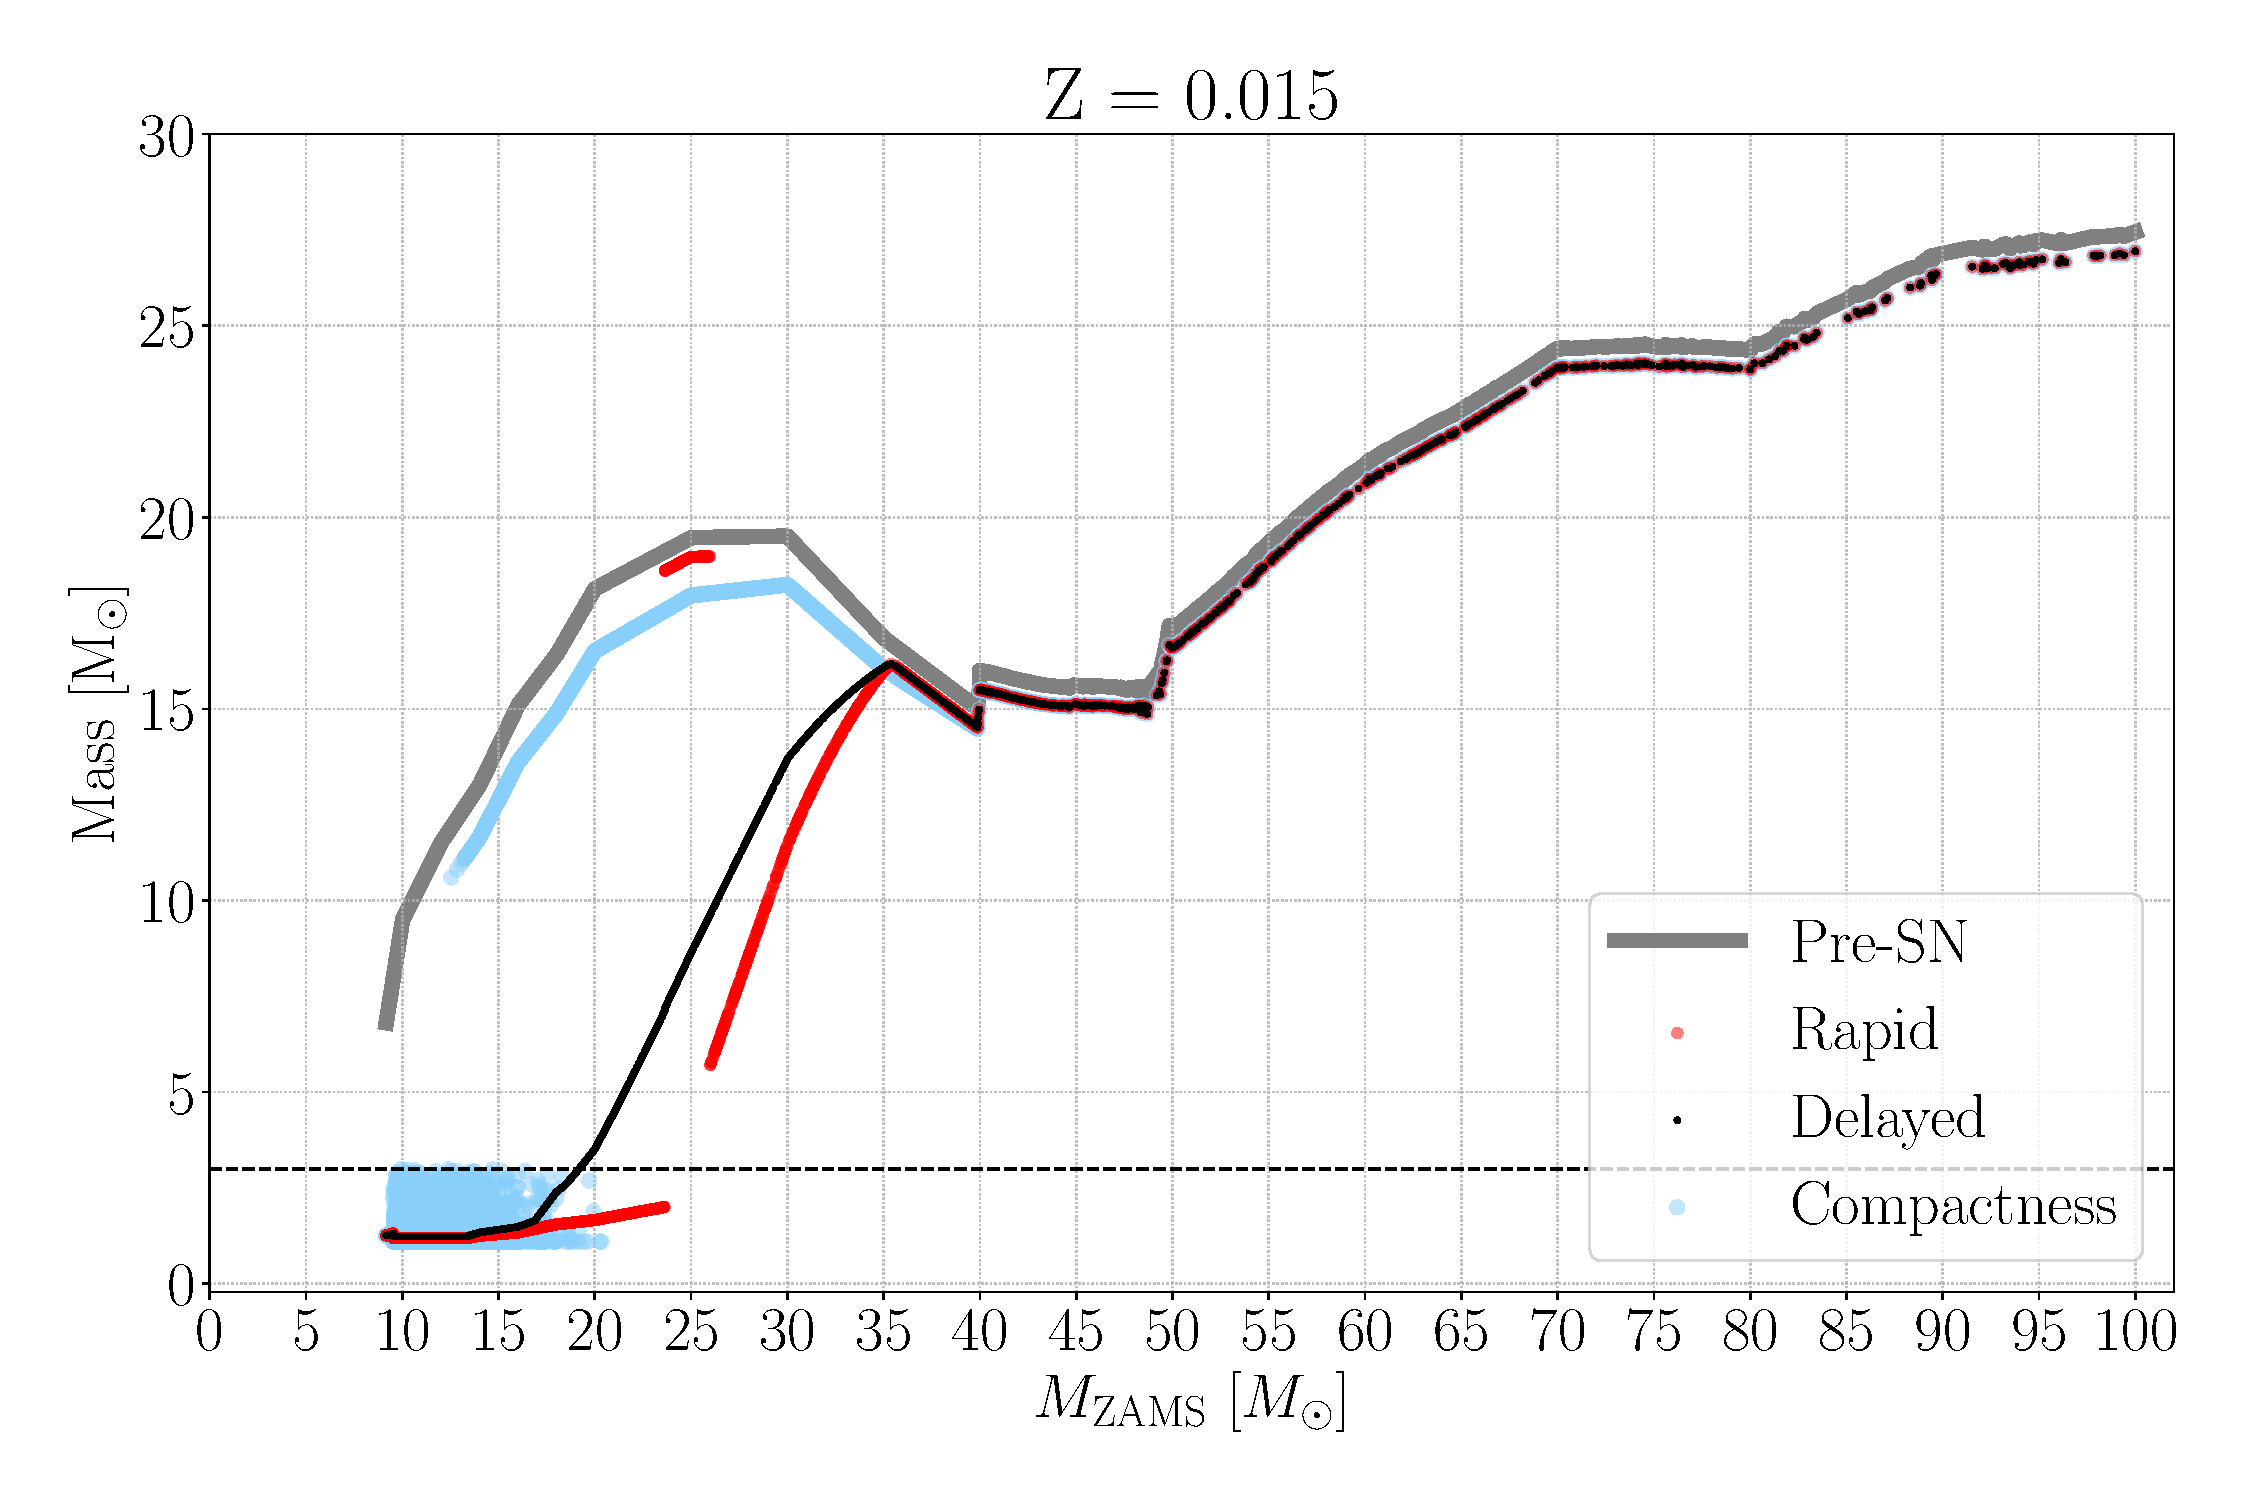
\includegraphics[width=1.05\textwidth]{./images/remnants_Z015.pdf}
	\end{minipage}
	\hfill
	\begin{minipage}{.40\textwidth}
		\centering
		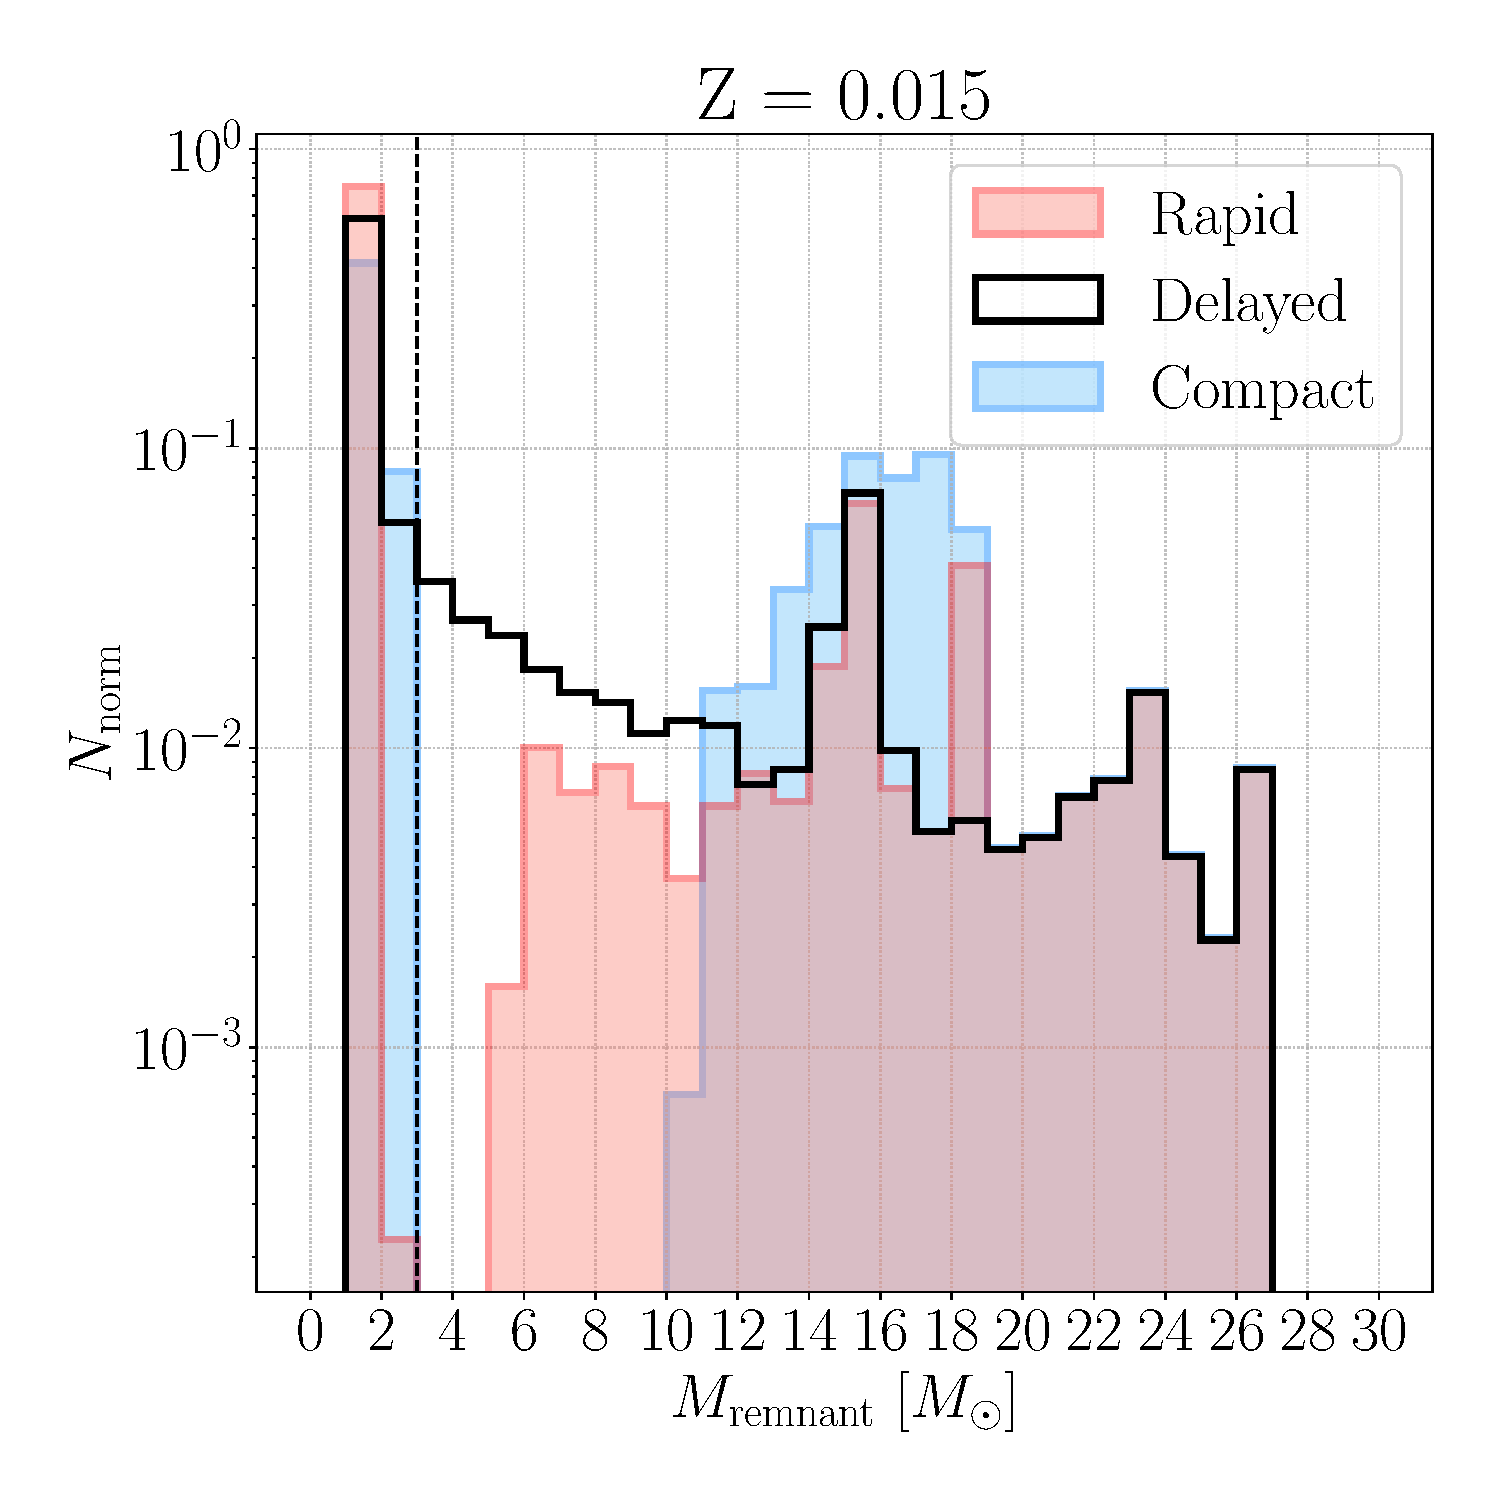
\includegraphics[width=1.05\textwidth]{./images/hist_Z015.pdf}	
	\end{minipage}
	\caption{Compact object masses for \emph{rapid} (red), \emph{delayed} (black) and \emph{compactness} (blue) CCSN models implemented in \texttt{SEVN} for the two solar metallicities adopted in this thesis: $Z=0.02$ (\emph{top}) and $Z=0.015$ (\emph{bottom}). \emph{Left:} Gray thick line shows the pre-SN mass as a function of the initial progenitor mass $\mzams$. The \emph{compactness} model produces relatively heavy black holes even from light progenitors, without the abrupt jumps exhibited by the \emph{rapid} model and the strong sensibility on the CO mass also shown by the \emph{delayed} model. \emph{Right:} PDFs of the compact object masses obtained simulating with \texttt{SEVN} $10^4$ stars extracted from a Kroupa initial mass function (see Sec.\ \ref{sec:initialconditionsSEVN}). The limited sample caused the non-physical gaps at $M_{\rm rem} \sim 11~\msun$ for $Z=0.02$ and the less dense points in the left-hand panel towards higher masses. In contrast, the \emph{rapid} model reproduces the putative low-mass gap $M_{\rm rem} \sim 2-5~\msun$ \cite{massgapreal_ozel2010}. Black dashed line at $3~\msun$ discriminates between neutron stars and black holes \cite{NSreview}. }\label{fig:remnants}
\end{figure}


\paragraph{Compactness} The \emph{compactness} model is based on the compactness parameter $\xi_\mathrm{2.5}$ introduced by O'Connor \& Ott \cite{Oconnor2011_compactness} to describe the ratio between a reference mass ($2.5~\msun$ here) and the radius that encloses such mass at the onset of the core-collapse

\begin{equation}\label{eq:compactness}
\xi_\mathrm{2.5}= \frac{2.5}{R(2.5 ~\msun)}
\end{equation}

Limongi \& Chieffi \cite{Limongi2018_rotatingCOcompactness} used their \texttt{FRANEC} stellar evolution code to probe the strong correlation between the compactness parameter and the CO mass at the onset of the core-collapse, finding that it was not significantly affected by stellar rotation. Mapelli et al.\ \cite{mapelli2020_compactness} interpolated the same \texttt{FRANEC} models to extract a fitting formula implementable in population-synthesis codes

\begin{equation}\label{eq:compactnessCOinSEVN}
	\xi_{2.5} = 0.55 -1.1 \left(\frac{1 \msun}{M_{\rm CO}}\right)
\end{equation}

Indeed, at the end of the CO burning, \texttt{SEVN} uses this formula to extract the compactness parameter of the star $\xi_*$. However, studies like the one carried out Ertl et al.\ \cite{Ertl2016}, showed that there is not a one-to-one correlation between a given compactness value and the possibility that the star successfully explodes as a CCSN or fails and the upper layers directly fall back to the proto-compact object. In particular,  Patton \& Sukhbold \cite{COcollapse} used hydrodynamics calculations and extracted the probability distribution shown in Fig.\ \ref{fig:compactness} to determine the explodability of a star given its compactness. Therefore, in the \emph{compactness} model, \texttt{SEVN} randomly draws a compactness value from the explodability distribution of Patton \& Sukhbold (the white filled one in Fig.\ \ref{fig:compactness}) and uses it as a threshold $\xi_c$: if the star is more compact it collapses forming a black hole ($\xi_* > \xi_c$) otherwise it explodes and produces a neutron star.

While the neutron star mass is randomly assigned according to the observed distribution of neutrons stars in binary systems \cite{mapelli2020_compactness}, the baryonic black hole mass is derived similarly to Fryer et al.\ \cite{Fryer2012} but substituting the role of the CO core with the He core

\begin{equation}\label{eq:massBHcompactness}
    M_{\rm BH, bar} = M_{\rm He} + f_{\rm H} (M_{\rm pre-SN}-M_{\rm He}),
\end{equation}

where $f_H \in [0,1]$ is the fallback parameter and accounts for the hydrogen mass retained in the compact object. Even though the fiducial \texttt{SEVN} model (and the one adopted in this thesis) adopts $f_{\rm H} = 0.9$, Eq.\ \ref{eq:massBHcompactness} underlines that for a collapsing Wolf-Rayet star the baryonic black hole mass is precisely the pre-SN mass $M_{\rm pre-SN}=M_{\rm He}$. Finally, \texttt{SEVN} uses Eq.\ \ref{eq:neutrinolosses} to account for neutrino losses and to convert the baryonic compact remnant mass into the gravitational one. 

Regardless of the explosion/implosion mechanism, \texttt{SEVN} will always  classify a compact object as a black hole (neutron star) if its mass is higher (lower) than the maximum mass allowed for a neutron star $M_{\rm NS,max} = 3~\msun$ \cite{NSreview,spera2019_mergingBBH}, indicated with a black dashed line in the panels of Fig.\ \ref{fig:compactness}.

\begin{figure}
	\centering
	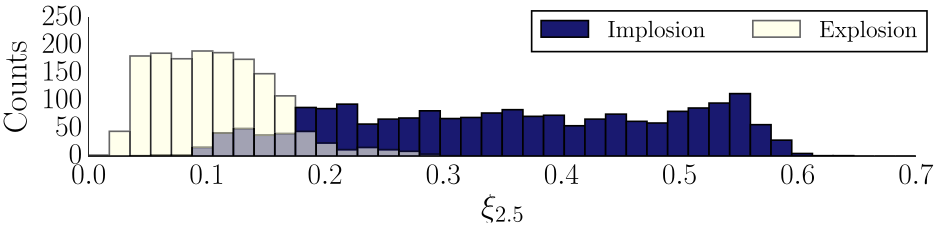
\includegraphics[width=.9\textwidth]{./images/compactness.png}	
	\caption{Explodability (white) and implodability (blue) probability distribution functions for the compactness parameter $\xi_{2.5}$ extracted by Patton \& Sukhbold \cite{COcollapse}. \texttt{SEVN} randomly draws a threshold compactness $\xi_C$ from the explodability distribution \cite{mapelli2020_compactness}.}\label{fig:compactness}
\end{figure}


\paragraph{Model comparison} Fig.\ \ref{eq:compactness} highlights the main differences in the CCSN models: even though the figures are built for the solar metallicity adopted in this thesis, the features and trends are characteristic of the models. I obtained the panels simulating with \texttt{SEVN} $10^4$ stars up to $\mzams = 100~\msun$, thus forming black holes only up to $\sim 21~(26)~\msun$ (the higher the metallicity, the more efficient the stellar winds and the lighter the compact remnants).

Looking at the left-hand panels, the \emph{compactness} model not only produces more massive compact objects but allows their formation from progenitors down to $\mzams \sim 13~\msun$, whereas the \emph{delayed} model stopped at $\mzams \sim 20~\msun$ and the \emph{rapid} model at $\mzams \sim 25~\msun$. If Fryer et al.\ \cite{Fryer2012} models produce a discontinuous distribution in the compact remnant masses due to the complicate dependence on the CO mass, the randomness introduced in the \emph{compactness} model allows stars with $\mzams \sim 13-20~\msun$ to produce a black hole or a neutron star. However, since the explodability distribution of Fig.\ \ref{fig:compactness} is shifted towards lighter masses, the \emph{compactness} model favours the production of black holes for progenitors in this intermediate region. Discrepancies between the three models vanish for $\mzams \gtrsim 40~\msun$, i.\ e.\ for exploding Wolf-Rayet stars of $\gtrsim 10-15~\msun$ (see also the right-hand panel of Fig.\ \ref{fig:masslostWR}). Such massive stars always implode and have CO core mass $M_{\rm CO} \gtrsim 11~\msun$, thus the only mass lost in the CCSN is the one carried away by neutrinos according to Eq.\ \ref{eq:neutrinolosses}. 

The right-hand panels highlight over-densities and gaps in the compact-object mass distribution. The \emph{rapid} model does not produce compact objects with $M_{\rm rem} \sim 2-5~\msun$, in agreement with the putative low-mass gap suggested by observations carried out in the Galaxy \cite{massgapreal_ozel2010}. In contrast, the \emph{delayed} model shows a continuous distribution of compact objects. Finally, the \emph{compactness} model produces an even larger low-mass gap between $\mzams \sim 3-8(10)~\msun $ for stars with metallicity $Z=0.015~(0.02)$. This gap is produced by stars with $\mzams \lesssim 13~\msun$ that are too light to collapse, therefore they explode and form a neutron star.





\subsection{Supernova kicks}\label{subsec:kicksSEVN}
\paragraph{Natal kicks} After a supernova event, the resulting compact object receives a natal kick formed by the combination of a Blaauw kick and a supernova kick. The first one, proposed by Blaauw in 1961 \cite{Blaauw1961}, is a $\lesssim 50$ km/s kick acting on the binary center of mass and is caused by asymmetries in the mass lost by the system as a whole \cite{Mandel2016_kicks}. Instead, the supernova kick is the one received directly by compact objects formed after successful supernova explosions and, similarly, is caused by asymmetries in the (baryonic or neutrino) mass ejection. 


Many efforts have been put in deriving a representative distribution of compact object natal kicks from observations, but still none of the proposed models seems to offer a complete picture. Hobbs et al.\ \cite{Hobbs2005} measured the proper motions of 233 Galactic pulsars, among which 56 young pulsars, finding that the velocity distribution of the latter can be modelled with a one-dimensional Maxwellian with root-mean-square of $\sigma = 265$ km/s. In contrast, Verbunt et al.\ \cite{Verbunt2017_bimodalkicks} adopted updated measurements and Bayesian analysis to argue that pulsar velocities follow a bimodal Maxwellian distribution with peaks at 120 and 540 km/s. More recently, Atri et al.\ \cite{Atri2019_kicks} studied proper motions of 16 black holes in X-ray binaries, finding that their velocity distribution is described with a Gaussian  curve with mean at 107 km/s: a probability distribution function (PDF)  very similar to the low-velocity peak indicated by Verbunt et al.\ \cite{Verbunt2017_bimodalkicks}.\\

\texttt{SEVN} includes both Blaauw and supernova kicks into its natal kick calculation. In the next paragraphs, I will discuss the supernova kick models that I adopted in this thesis and that are derived from the \emph{hobbs pure}, \emph{hobbs} and \emph{unified} options available in \texttt{SEVN} (for the implementation of Blaauw kicks see Iorio et al.\ in preparation).


\paragraph{Hobbs pure } Following the  observations of Hobbs et al.\ \cite{Hobbs2005}, the \emph{hobbs pure} option draws a random supernova kick from a one-dimensional Maxwellian curve with root-mean-square $\sigma$ as free parameter. The default value $\sigma = 265$ km/s reproduces the observed pulsar velocity distribution. In this thesis, also $\sigma = 70$ km/s will be considered for this option, since it is the root-mean-square correspondent to a Maxwellian curve with median in 107 km/s that can reproduce the distribution of black hole supernova kicks found by Atri et al.\ \cite{Atri2019_kicks}.

\paragraph{Hobbs} The \emph{hobbs} option draws a random kick $f_{\sigma}$ from a one-dimensional Maxwellian as in the \emph{hobbs pure} option, but scales it accounting for the fraction $f_{\rm fb}=M_{\rm fb}/(M_{\rm rem} - M_{\rm proto})$ of matter falling back to the proto-compact object.

\begin{equation}\label{eq:kickhobbs}
    v_{\rm kick, h} = f_\sigma\,{} (1-f_{\rm fb}) 
\end{equation}

The fallback parameter adopted here $f_{\rm fb}$ accounts for the mass ejected in the supernova explosion and for the neutrinos losses. In particular, $f_{\rm fb}$ is calculated with the gravitational compact remnant mass of Eq.\ \ref{eq:neutrinolosses} and is sensible to the baryonic compact remnant mass. The latter is obtained through a different fallback parameter, that, depending on the CCSN model, is a function of the CO mass or is fixed a-priori.
% informazione avuta parlando con Giuliano


\paragraph{Unified}  Giacobbo \& Mapelli \cite{SNkicksUnified_Giacobbo2020} introduced an alternative model to describe supernova kicks through linear momentum conservation, calculating the kick velocity with

\begin{equation}\label{eq:kickunified}
    v_{\rm kick, un} = f_{\sigma} \frac{M_{\rm ej}}{\langle M_{\rm ej}\rangle} \frac{\langle M_{\rm NS}\rangle}{M_{\rm rem}}
\end{equation}


As in the \emph{hobbs} option, the kick is drawn from a Maxwellian distribution ($f_{\sigma}$) and then down-scaled to account for the mass lost in the supernova explosion. Here, an argument based on linear momentum conservation suggests that the natal kick should scale with $M_{\rm rem}^{-1}$. Similarly, the linear scaling with the mass of the ejecta $M_{\rm ej}$ is the simplest way to account for the fact that natal kicks originate from asymmetries in the ejecta \cite{BrayEldridge2016_natalkicksunified}. This approach has two main advantages: it works for both neutron stars and black holes and it naturally accounts for the low natal kicks originating from stripped and ultra-stripped supernovae, according to recent models \cite{tauris2017_formationnatalkicks}.\\

The ejected mass $M_{\rm ej} = M_{\rm pre-SN} - M_{\rm rem}$ is calculated as the difference between compact remnant and pre-SN mass. As for the \emph{hobbs} option, \texttt{SEVN} uses as compact remnant mass $M_{\rm rem}$ the gravitational one, obtained after the neutrino losses and calculated with Eq.\ \ref{eq:neutrinolosses}. However, unlike \emph{hobbs}, the \emph{unified} model makes an exception for black holes formed with the \emph{compactness} CCSN and fallback $f_{\rm H}=1$: only for this case, it assumes that the supernova kick is quenched and sets it to zero.
% informazione avuta parlando con Giuliano

In eq.~\ref{eq:kickunified}, $\langle{}M_{\rm ej}\rangle{}$ and $\langle{}M_{\rm NS}\rangle{}$ are two factors of normalization, corresponding to the average mass of the ejecta and to the average neutron star mass, respectively. They are calibrated at $Z=0.02$ in order to reproduce the natal kick distribution of Hobbs et al.\ \cite{Hobbs2005}. For the CCSN models considered here, the calibrated average values are: $\langle M_{\rm NS}\rangle = 1.27~\msun$ and $\langle M_{\rm ej}\rangle = 10.9~\msun$ if \emph{rapid}, $\langle M_{\rm NS}\rangle = 1.36~\msun$ and $\langle M_{\rm ej}\rangle = 10.45~\msun$ if \emph{delayed} and $\langle M_{\rm NS}\rangle = 1.33~\msun$ and $\langle M_{\rm ej}\rangle = 10.45~\msun$ if \emph{compactness} (see Iorio et al.\ in preparation).
% i valori medi di NS e ejecta sono in src/general/params.cpp mentre MNS = 1.33 per il compact è la media della gaussiana usata per estrarre le NS masses







\subsection{Orbital parameters after a supernova}\label{subsec:SEVNpostsupernovaorbit}
\paragraph{Mass loss always modifies the orbit} After a supernova explosion, a binary system \emph{always} loses mass (at least the one carried away by neutrinos, see Eq.\ \ref{eq:neutrinolosses}) and this results in a kick on the center of mass (the Blaauw kick, see Sec.\ \ref{subsec:kicksSEVN}). Following Hurley et al.\ \cite{Hurley2002} prescriptions for \texttt{BSE}, \texttt{SEVN} assumes that the supernova explosion is instantaneous and does not change the separation between the two orbiting objects, thus, a change in the total mass of the binary system modifies its semi-major axis and eccentricity. Of course, the new orbital parameters will show larger differences with respect to the old ones if the resulting compact object receives also a supernova kick. In particular, this is the case of all the systems simulated in this thesis: I chose $f_{\rm H}=0.9$ for the \emph{compactness} CCSN model and remind that \emph{rapid} and \emph{delayed} models always allow a kick (see Sec.\ \ref{subsec:kicksSEVN}).

\paragraph{Routine for parameter determination} The routine adopted by \texttt{SEVN} is the same as described in Appendix A2 of Hurley et al.\ \cite{Hurley2002}. Here, I summarize the main assumptions.

First of all, \texttt{SEVN} calculates the new compact object relative velocity $v_{\rm n}$ summing up Blaauw and supernova kick (if present) magnitudes. The supernova kick is randomly extracted according to one of the models described in Sec.\ \ref{subsec:kicksSEVN} and then is projected according to an uniform probability distribution over all solid angles. Moreover, the routine randomly calculates also the position in the orbit where the compact object formed, with Kepler's second law suggesting that is more probable that the supernova occurred in the apocenter. The explosion position eventually determines the compact object separation $r$ from the companion. Assuming that the supernova is instantaneous, thus $r$ is not modified, the new semi-major axis $a_{\rm n}$ is determined by the new relative velocity and reduced total binary mass $M_{\rm b} = M_{\rm rem} + M_{\rm companion}$

\begin{equation}\label{eq:neworbitalseparation}
    v_{\rm n}^2 = G M_{\rm b} \left( \frac{2}{r} - \frac{1}{a_{\rm n}} \right)
\end{equation}

Assuming that the specific orbital angular momentum is conserved throughout the explosion, the new semi-major axis determines also the new eccentricity $e_{\rm n}$ 

\begin{equation}\label{eq:neweccentricity}
    G M_{\rm b} a_{\rm n} (1-e_{\rm n}^2) = |\vec{r} \times \vec{v}_{\rm n}|^2
\end{equation}

\section{Initial conditions}\label{sec:initialconditionsSEVN}
In this thesis, I generated 24 sets of $10^6$ representative binary populations to explore some of the most relevant sources of uncertainties in their evolution (e.g., metallicity, core-collapse supernova and kick models). 

\subsection{Parameter space}\label{subsec:parameterspace}
\paragraph{Explored} All combinations of parameters and models explored in the simulated sets are reported in Fig.\ \ref{fig:parameterspace}: each set is defined with a metallicity, CCSN and kick model.\\

I chose to explore two slightly different possible values of the solar metallicity because, even if $Z=0.015$ is the more accurate calibration \cite{caffau2011solarmetallicity}, $Z=0.02$ is still the standard one adopted in the literature, therefore it allowed me to carry on a more self-consistent comparison with previous results. Moreover, \texttt{PARSEC} tables are generated with tracks at $Z=0.02$ and $Z=0.014$ for ``normal'' stars and tracks at $Z=0.02$ and $Z=0.01$ for pure-He stars. Therefore, choosing $Z=0.02$ allows to interpolate only in the masses while choosing $Z=0.015$ requires \texttt{SEVN} to interpolate stellar properties both weighting the nearest tracks in mass and metallicity (see Sec.\ \ref{subsec:SEVNproperties} for more details on \texttt{SEVN} interpolation method).\\

As shown in Fig.\ \ref{fig:remnants} and discussed in Sec.\ \ref{subsec:SNmodels}, the \emph{rapid}, \emph{delayed} and \emph{compactness} models for core-collapse supernovae are very different in the assumptions and compact remnant masses. Choosing one model or another will  significantly affect the binary black hole demography and their evolutionary channels. Therefore, I adopted all the three models to probe their effect and test if, nevertheless, some features were common.\\

Finally, in Sec.\ \ref{subsec:kicksSEVN} and \ref{subsec:SEVNpostsupernovaorbit} I showed that there is not an unique model for supernova kicks and that different kick magnitudes affect the orbital properties of binaries after the supernova event, determining their survival as bound systems and their possibility to merge via gravitational wave emission within a Hubble time. Therefore, I compared the \emph{unified}, \emph{hobbs} and \emph{hobbs pure} options to study the impact of different kick models, also considering different values for the $\sigma$ parameter (see Fig.~\ref{fig:parameterspace}). % scaling to kicks randomly extracted from the same standard Maxwellian of Hobbs et.\ al \cite{Hobbs2005}, derived from pulsar proper motions and defined by rms of $\sigma=265$ km/s. Moreover, only for the \emph{hobbs pure} option (the only one that does not scale the kick amplitudes), I tested possible differences with kicks extracted from the more representative black hole kick distribution of Atri et al.\ \cite{Atri2019_kicks}: a Maxwellian with $\sigma=70$ km/s.} 




\begin{figure}
	\centering
	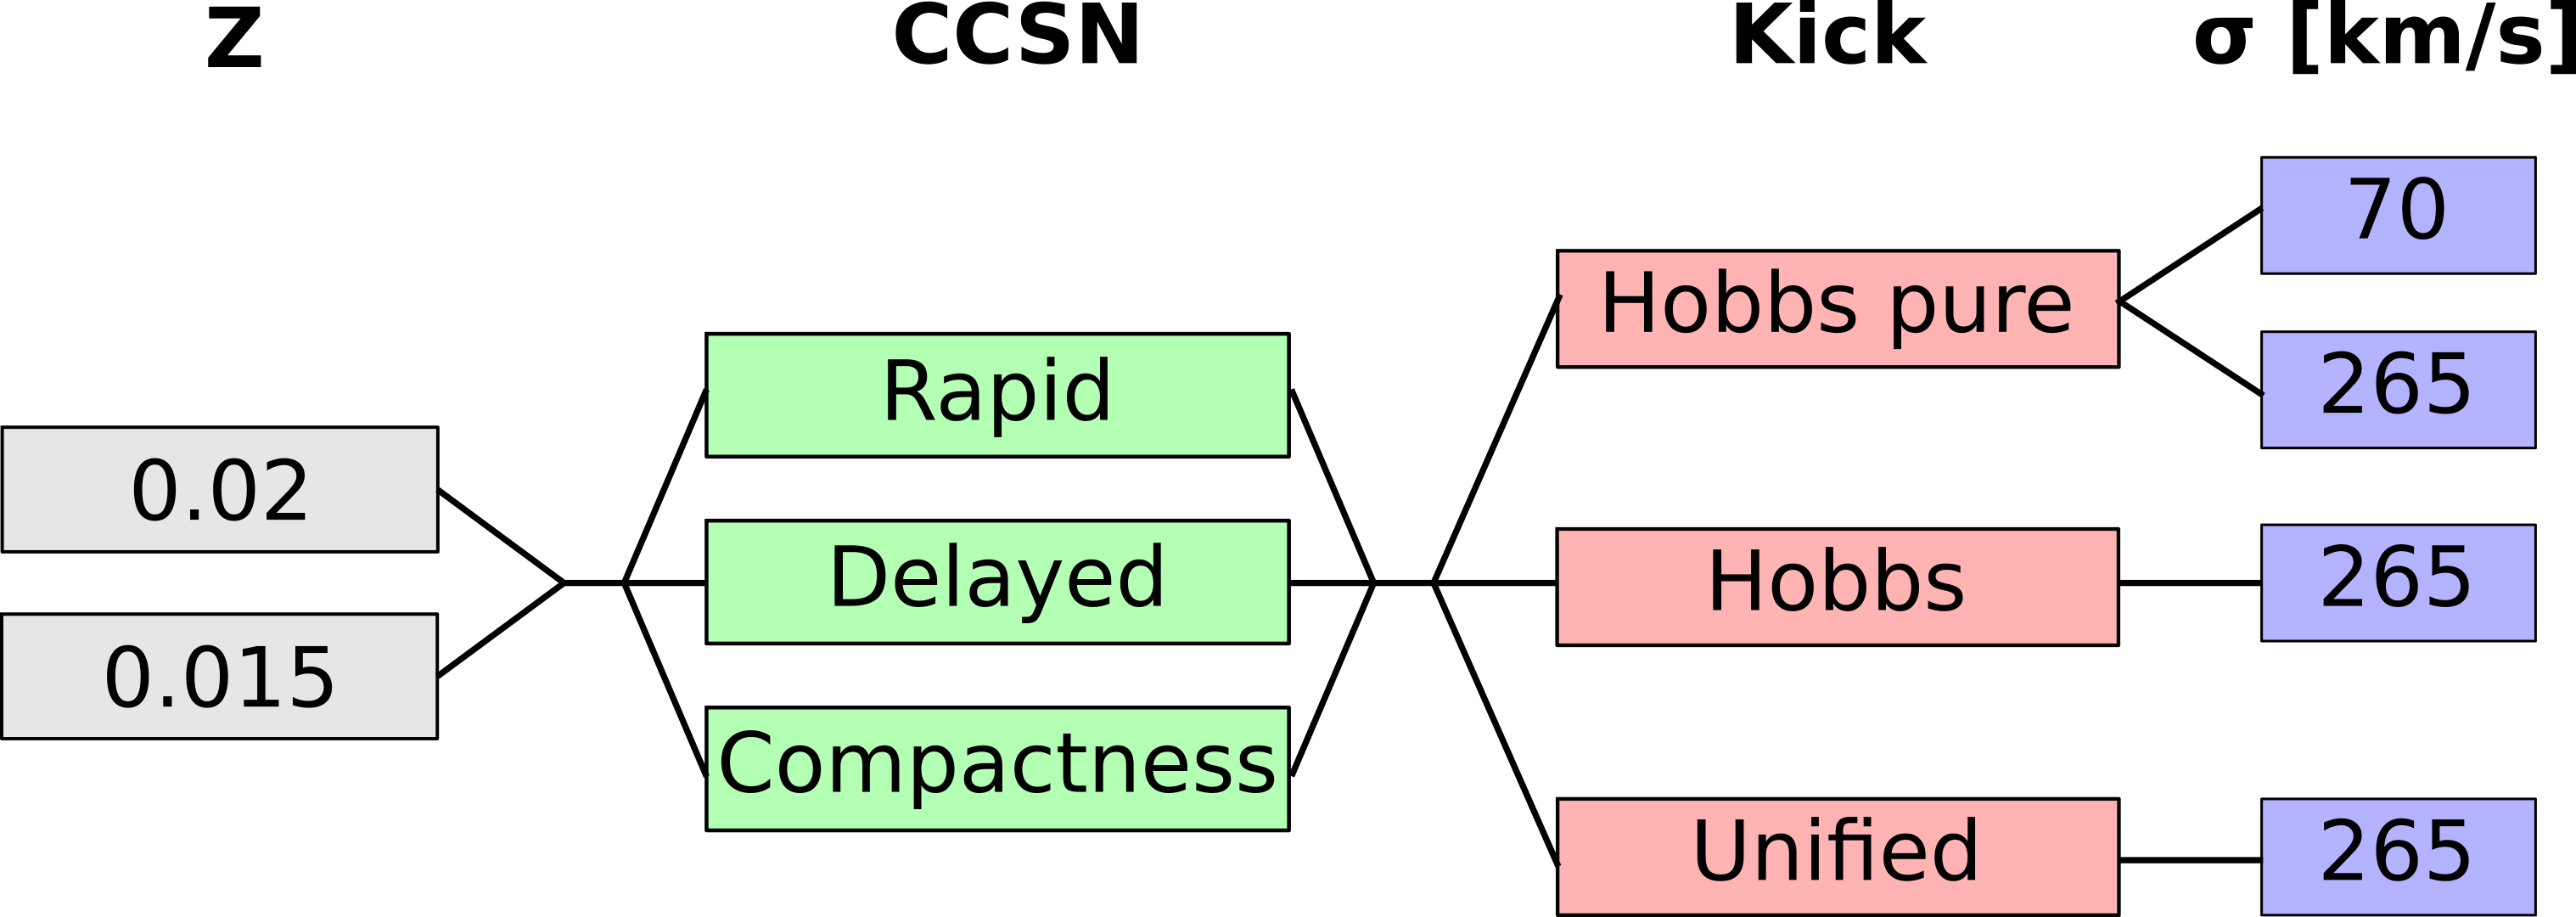
\includegraphics[width=.95\textwidth]{./images/parameterspace.png}	
	\caption{Schematic representation of the 24 combinations of the parameter space explored in this thesis. Each set explores binary black hole formation assuming a solar metallicity value ($Z=0.02$ or $Z=0.015$), core-collapse model for the supernova explosion (\emph{rapid}, \emph{delayed} or \emph{compactness}, see Sec.\ \ref{subsec:SNmodels}) and supernova kick prescription (\emph{hobbs pure}, \emph{hobbs} or \emph{Unified}, see Sec.\ \ref{subsec:kicksSEVN}). Kick velocities are generally drawn from a Maxwellian with root-mean-square $\sigma = 265$ km/s following the pulsar proper motions observed by Hobbs et al.\ \cite{Hobbs2005}. For comparison and only for kicks drawn from a pure Maxwellian (\emph{hobbs pure}), I also tested the option with lower kick values extracted from a Maxwellian with $\sigma = 70$ km/s,  representative of the black hole proper motion observed by Atri et al.\ \cite{Atri2019_kicks}.}\label{fig:parameterspace}
\end{figure}


\paragraph{Fixed}
Mass transfer prescriptions also significantly affect the binary black hole demography. As already discussed in Sec.\ \ref{subsec:Rochelobeoverflow} and \ref{subsec:Commonenvelope}, current models need to be revised and are probably too much simplified and imprecise to describe a process so complex. Knowing that, I chose not to explore also this parameter space and instead I adopted the fiducial settings that were tuned in \texttt{SEVN} to reproduce the merger rates observed by the LIGO-Virgo Collaboration (see Iorio et al.\ in preparation). \\

For the common envelope evolution, the fiducial $\alpha \lambda$ prescription adopts $\alpha=5$ and $\lambda$ from fits of Claeys et al.\ \cite{Clayes2014_lambdaCE}. I point out that, even though Claeys et al.\ report different $\lambda$ values for different evolutionary stages, they do not provide a fit for pure-He stars: for them, \texttt{SEVN} adopts $\lambda_{\rm WR} = 0.5$.

For Hertzsprung-gap stars donors entering an unstable Roche lobe overflow, I adopted the \emph{pessimistic} option anticipated in Sec.\ \ref{subsec:masstransferSEVN}: I assumed that the core-envelope separation is not yet well-defined, preventing similar stars to possibly survive a common envelope, thus, merging them with the companion. A similar assumption follows the results of Gallegos-Garcia et al.\ \cite{gallegos2021MESAvspopsynth} shown in Fig.\ \ref{fig:MESAvsPopsynth}, which pointed out that current population-synthesis codes are likely over-estimating the number of binary black holes formed from H-rich donor stars that survived a common envelope evolution.\\

Finally, I point out that I evolved non-rotating stars: both the initial spins were set to zero and the \texttt{PARSEC} tables adopted were obtained from non-rotating stars.



\subsection{Generating binary sets}\label{subsec:setgeneration}
\paragraph{Reproducibility} According to the \texttt{SEVN} formalism, each set of binary systems is evolved according to an a-priori defined supernova kick model. The input is a list of binaries, each with specified initial conditions:  initial metallicity, mass, spin and core-collapse supernova model; binary initial semi-major axis, eccentricity, and random seed. In particular, the  random seed is used to draw the natal kick and allows to reproduce  the same simulated system, extracting the same random kick from a pre-selected Maxwellian. 

In this thesis, I used the \texttt{IC4popsyn} package developed by Nicola Giacobbo \footnote{\url{https://github.com/GiacobboNicola/IC4popsyn}} to generate the initial set of binaries with the formalism required by \texttt{SEVN} inputs and adopting the initial distributions described in the next paragraphs. To allow a better comparison between sets characterized with different models, I generated only once the list of initial conditions for the $10^6$ binaries, later changing only the values of metallicity or core-collapse model. By doing so, I made sure to evolve always the same binary population (i.\ e.\ same initial masses for the same semi-major axis, eccentricity, period and random seed), only under different conditions for metallicity, CCSN or kick model.

\paragraph{Initial masses} I generated the masses of the primary stars $M_1 \geq M_2$ following the Kroupa \cite{Kroupa2001} Initial Mass Function (IMF), limited to the massive stars that could be black hole progenitors

\begin{equation}
	\xi(M_1) \propto M_1^{-2.3} \qquad M_1 \in [10,150]~\msun 
\end{equation}

I chose the lower boundary of $M_\textup{1,min} = 10~\msun$ as a compromise between the need to simulate stars with $\mzams \lesssim 25~\msun$, able to accrete mass from the companion and form a black holes, and the need to obtain secondaries with values included in the \texttt{PARSEC} tables, i.e. $M_2 > 2.2~\msun$ (see Sec.\ \ref{subsec:SEVNproperties}).

I obtained the distribution of the secondary masses $\xi(M_2)$ from the primary $\xi(M_1)$ and mass ratio $\xi(q)$ distributions, where $q=M_2/M_1$. In particular, I adopted the distribution proposed by Sana et al.\ \cite{Sana2012} that was derived from binaries containing O-type stars sampled in six Galactic open clusters

\begin{equation}
\xi(q) \propto q^{0.1} \qquad \quad ~q \in [0.1,1] 
\end{equation}

obtaining

\begin{equation}
\xi(M_2) = \xi(M_1) \,{} \xi(q)  \qquad  M_2 \in [1 ~\msun , M_1]
\end{equation}

%Similarly to before, the minimum value $q_\textup{min}=0.1$ is a calibrated compromise that allows to explore all the reasonable mass combinations without producing too many secondaries below the \texttt{PARSEC} tables threshold of $M_2 > 2.2~\msun$. In this case, the $M_\textup{1,min} = 10~\msun$ results in a $M_\textup{2,min} = 1 < 2.2~\msun $; therefore I had to generate $1.10 \times 10^6$ binaries in order to simulate $\sim 1.04 \times 10^6$ systems. Nevertheless, the $\sim 6 \times 10^4$ systems not simulated will not affect this thesis conclusions, since masses so low would not have produced a black hole or have resulted in a binary black hole under any circumstance.

\paragraph{Periods and eccentricities} I used the  distributions from Sana et al.\ \cite{Sana2012} to  generate the initial orbital period $P$. In particular, I adopted their distribution for the logarithmic orbital periods $\mathcal{P} = \log(P/\text{days})$

\begin{equation}
	\xi(\mathcal{P}) \propto \mathcal{P}^{-0.55} \qquad \mathcal{P} \in [0.30,5.5]
\end{equation}
% boundaries in terms of usual period P in days correspond to Pmix = 1.41 days and Pmax = 316 227 days = 866 yrs

I followed the prescriptions of Moe \& Di Stefano \cite{MoeDiStefano2017} and set $P=2~$days ($\mathcal{P}=\log(P=2)=0.3$) as the lower limit for the period distribution, assuming that binaries with shorter period already circularized. In fact, Moe \& Di Stefano showed that there is a complex correlation between the mass ratio $q$, period $P$ and eccentricity $e$ of early-type binaries containing O-type and B-type main sequence stars. Even though I assumed that $q$ and $P$ distributions are independent for simplicity, I tried to account for it correlating $P$ and $e$ following their suggested prescription

\begin{equation}
	\xi (e (P)) \propto 1-(P/\text{days})^{-2/3} \qquad P \geq 2~\text{days}
\end{equation}






%%%%%%%%%%%%%%%%%%%
%% Chapter 4 %%%%%%
%%%%%%%%%%%%%%%%%%%

\chapter{Results}\label{sec:results}

\paragraph{Chapter outline} In this chapter I will present the results of the 24 simulation sets, each composed of $10^6$ binaries, that I simulated with the population-synthesis code \texttt{SEVN} according to the assumptions described in Sec.\ \ref{sec:initialconditionsSEVN}. I will probe the role of Wolf-Rayet--black hole systems (hereafter, WR--BHs) as progenitors of binary black holes (BBHs) and, in particular, as progenitors of BBHs that can merge via emission of gravitational waves within a Hubble time (GW--BBHs). I will discuss the impact of the parameter space on the results, in particular the role of metallicity $Z$, core-collapse supernova and natal kick models. 

I will explore in detail the evolution of Cyg X-3: the only known WR--BH candidate in the Milky Way. To identify a Cyg X-3 candidate, I adopted the measurements obtained  by Koljonen et al.\ \cite{CygX-3_Koljonen2017} discussed in Sec.\ \ref{subsec:cygx3observations}: Wolf-Rayet mass of $M_{\rm WR} = 8-14~\msun$, black hole mass of $M_{\rm BH}=3-10~\msun$ and period of $P=4.5-5.1$ hours. Even though the period was accurately measured to be $P=4.8$ hours with a millisecond precision, I arbitrarily set an interval of $\pm 0.3$ hours to be sure to sample enough representative systems with properties similar to Cyg X-3.

%%\paragraph{A complementary appendix} To facilitate the reading and the discussion, I will collect most of the figures and plots in Appendix \ref{app:figures} and propose only the most relevant ones in the main text, along with a summary table. 



\section{WR--BHs as BBHs and GW--BBHs progenitors at $\mathbf{Z_\odot}$} \label{sec:roleWRBH}


In Tab.\ \ref{tab:simulationresults} I reported the results of all the simulations carried out in this thesis, grouping them according to the supernova kick model; from top to bottom: \emph{hobbs pure} (with Maxwellian root-mean-square $\sigma$ of $70$ and $265$ km/s, respectively, for the first two tables), \emph{hobbs} and \emph{unified} (both with $\sigma=265$ km/s).

\subsection{WR--BHs: a key intermediate configuration} 
\paragraph{Almost a necessary phase to form GW--BBHs} The results collected in Tab.\ \ref{tab:simulationresults} indicate that BBHs and GW--BBHs are rare at solar metallicity: only $\sim 0.01 - 10$\% of the simulated systems form binary black holes and the fraction is even lower for the BBHs that merge via emission of gravitational waves within a Hubble time, being less than $\lesssim 0.01$\% (with dips of only $\sim 0.001$\% for some combinations of the parameter space). 

My results show that nearly all the progenitors of BBHs and GW--BBHs must have become WR--BH systems at some point in their life. In fact, considering all the runs together, more than $\gtrsim 70\%$ of BBHs and $\gtrsim 90\%$ of GW--BBHs formed after a WR--BH configuration. These values are a conservative lower boundary determined by some sets, but Tab.\ \ref{tab:simulationresults} highlights that almost 100\% of the binaries in both categories evolved through the WR--BH phase.

\paragraph{A solid result} Even though the production efficiency of the systems of interest changes for different combinations of metallicity, CCSN and kick models, the fraction of BBHs and GW--BBHs evolved through a WR--BH phase is almost constant. Therefore, regardless on the combination of parameters adopted here, WR--BH binaries emerge as a fundamental and necessary intermediate configuration to produce BBHs and GW--BBHs at solar metallicity.

\subsection{Cyg X-3: a GW--BBH progenitor}
\paragraph{Cyg X-3 fate} The key role of WR--BH systems as progenitors of GW--BBHs is supported also by the fate of Cyg X-3. In fact, according to the models adopted in this work and reported in Tab.\ \ref{tab:simulationresults}, Cyg X-3 is expected to evolve producing a GW--BBH with a $\gtrsim 75 \%$ probability. 

The result is solid within the parameter space explored, even though our probability estimate is only indicative and strongly affected by the low number of samples, eventually caused by the limited period window (only $\Delta P \sim 40$ minutes) adopted to classify a system as Cyg X-3. Because of the low statistics (only two candidates, none of which merges), I excluded from the above percentage the set with $Z=0.02$, \emph{delayed} CCSN and \emph{hobbs pure} with $\sigma=265$ km/s model, even though I recognize that the \emph{delayed} model disfavours the formation of Cyg X-3 candidates due to a selection effect in the primary black hole mass (for a more detailed discussion see Sec.\ \ref{subsec:CygX3masstransferdrivenevo}).

\paragraph{A proxy for WR--BHs role?} In the next sections, Cyg X-3 will be used as a proxy to study in detail the formation channels of WR--BH systems as GW--BBHs. Even though Cyg X-3 properties will reproduce a sub-population of GW--BBHs (see Sec.\ \ref{sec:resultsCygX3evo}), its evolution will not represent \emph{all} WR--BH systems forming a BBH or a GW--BBH. In fact, Cyg X-3 relevance changes with different combinations of the parameter space and is of $\sim 1-0.0001\%$  and  $\sim 1.5 - 35 \%$ for WR--BHs forming BBHs and GW--BBHs, respectively.


\begin{table}[htbp!]
    \centering
    \begin{tabular}{l >{\hspace{2pc}}r>{\hspace{0.47pc}}r>{\hspace{0.47pc}}r >{\hspace{3pc}}r>{\hspace{0.47pc}}r>{\hspace{0.47pc}}r} %1.2 pc left  % 1pc, 2pc
        \toprule
        Metallicity & \multicolumn{3}{c}{$Z=0.02$} & \multicolumn{3}{c}{$Z=0.015$}  \\
		%\midrule
		CCSN model & Rap & Del & Com &  Rap & Del & Com\\
		\toprule
		\toprule
		Natal kick model & \multicolumn{6}{c}{Hobbs pure ($\sigma{}=70$ km/s)}
		\\
		\toprule
		BBHs  		                    & 5626 & 5248 & 18425 & 10350 & 7564 & 27740 \\
		after a WR--BH			& 100\% & 100\% & 100\% & 99\% & 99\%& 100\% \\
		\hline
		GW--BBHs  						& 207 & 171 & 949 & 418 & 282 & 1287 \\
		after a WR--BH				& 207 & 171 & 948 & 418 & 281 & 1285 \\
		\hline
		Cyg X-3 candidates 	 		& 14 & 8 & 76 & 16 & 10 & 18 \\
		becoming GW--BBHs   			& 14 & 6 & 76 & 16 & 9 & 18 \\
		\bottomrule 	
	\end{tabular}%hobbspure70
	\vspace{0.3mm}
	\begin{tabular}{l >{\hspace{2pc}}r>{\hspace{0.72pc}}r>{\hspace{0.72pc}}r >{\hspace{3pc}}r>{\hspace{0.72pc}}r>{\hspace{0.72pc}}r}  %1.35 left
		\toprule
		Natal kick model & \multicolumn{6}{c}{Hobbs pure ($\sigma{}=265$ km/s)}\\
		\toprule
		BBHs                        & 166 & 156 & 727  & 416 & 260 & 1420 \\
		after a WR--BH	  & 100\% & 100\% &  100\% & 99\% & 99\%&  100\% \\
		\hline
		GW--BBHs  		          & 34 & 21 & 221 & 101 & 67 &  392\\
		after a WR--BH	  & 34 & 21 &  221& 101 & 67 &  392\\
		\hline
		Cyg X-3 candidates  	  & 4 & 2 & 29 & 6 & 4 &  7\\
		becoming GW--BBHs   	  & 4 & 0 & 23 & 5 & 3 & 7 \\
		\bottomrule 	
	\end{tabular}%hobbspure265
	\vspace{0.3mm}
	\begin{tabular}{l >{\hspace{2pc}}r>{\hspace{0.2pc}}r>{\hspace{0.2pc}}r >{\hspace{3pc}}r>{\hspace{0.2pc}}r>{\hspace{0.2pc}}r}
		\toprule
		Natal kick model & \multicolumn{6}{c}{Hobbs}\\
		\toprule
		BBHs                      		& 44307 & 35029 & 96557 & 55986 & 45701 & 109935 \\
		after a WR--BH			& 100\% & 100\% & 96\% & 92\% & 96\% & 94\% \\
		\hline
		GW--BBHs  						& 70 & 108 & 271 & 230 & 173 & 201 \\
		after a WR--BH			& 70 & 108 & 257 & 225 & 168 & 189 \\
		\hline
		Cyg X-3 candidates  	 		& 15 & 6 & 70 & 19 & 12 & 22 \\
		becoming GW--BBHs   		 	& 15 & 5 & 70 & 19 & 9 & 22 \\
		\bottomrule 	
	\end{tabular}%hobbs265
	\vspace{0.3mm}
		\begin{tabular}{l >{\hspace{2pc}}r>{\hspace{0.1pc}}r>{\hspace{0.1pc}}r >{\hspace{3pc}}r>{\hspace{0.1pc}}r>{\hspace{0.1pc}}r}
	    \toprule
		Natal kick model & \multicolumn{6}{c}{Unified}
		\\
		\toprule
		BBHs  		& 55655 & 46373 & 142613 & 71016 & 61257 & 157671 \\
		after a WR--BH	& 90\% & 95\% & 68\% & 87\% & 88\%& 69\% \\
		\hline
		GW--BBHs  		& 45 & 62 & 246 & 74 & 76 & 177 \\
		after a WR--BH	& 45 & 57 & 244 & 73 & 73 & 177 \\
		\hline
		Cyg X-3 candidates  	 & 16 & 7 & 70 & 19 & 9 & 22 \\
		becoming GW--BBHs   		 & 16 & 6 & 70 & 19 & 9 & 22 \\
		\bottomrule 	
	\end{tabular}%unified265
	\caption{Simulation results for each set of $10^{6}$ binaries generated with a different combination of metallicity, CCSN and kick models. The results are grouped by kick model, with abbreviated CCSN names. From top to bottom: \emph{hobbs pure} with $\sigma = 70$ km/s;  \emph{hobbs pure},  \emph{hobbs} and \emph{unified} with $\sigma = 265$ km/s (see Sec.\ \ref{sec:initialconditionsSEVN}).}\label{tab:simulationresults}
\end{table}





\section{Properties of BBHs and GW--BBHs}\label{sec:propertiesBBHsandGWBBHs}

\subsection{Progenitors}\label{subsec:progenitorsBBHsGWBBHs}
Figures\ \ref{fig:resultsM1prog}, \ref{fig:resultsM2prog}, \ref{fig:resultsqprog} and \ref{fig:resultsaprog} show the probability distribution functions of primary mass $M_{\rm 1,ZAMS}$, secondary mass $M_{\rm 2,ZAMS}$, mass ratio $q_{\rm ZAMS}=M_{\rm 2,ZAMS}/M_{\rm 1,ZAMS}$ and semi-major axis $a_{\rm ZAMS}$ at ZAMS for BBHs and GW--BBHs progenitors undergoing a WR--BH evolution. Here and in the following sections, I will indicate with the subscript 1 (2) all the quantities referred to the primary (secondary): the star initially more (less) massive and that, usually, becomes the progenitor of the black hole (Wolf-Rayet star) in the WR--BH configuration. % non sempre la secondaria diventa WR progenitor ma pochissime scambiano il loro ruolo (< 5 per set, e solo in alcuni di essi)

\paragraph{BBHs} BBH progenitor properties follow almost the same original distribution used to generate the initial conditions (see Sec.\ \ref{sec:initialconditionsSEVN}). The PDFs are compatible throughout the whole explored parameter space, except for systems evolved with supernova kicks drawn from a pure Maxwellian distribution (\emph{hobbs pure} option) similar to the one of Hobbs et al.\ \cite{Hobbs2005} (see Sec.\ \ref{subsec:kicksSEVN}). This kick model favours high kicks, thus breaking initially wide $a_{\rm ZAMS} \gtrsim 10^4~ \rsun$ and asymmetric systems $q_{\rm ZAMS} \lesssim 0.2$, allowing only binaries with secondaries $M_{\rm 2,ZAMS} \lesssim 90~\msun$. Similar strong kicks allow to survive only few black holes in a bound orbit, thus producing the lowest number of BBHs for any combination of metallicity and CCSN model (Tab.\ \ref{tab:simulationresults}). 


\paragraph{GW--BBHs} The PDFs of GW--BBH progenitors are more sensible to the parameter space, even if they also exhibit some common features: GW--BBHs formed through WR--BHs need to start their evolution from an orbit with initial semi-major axis $a_{\rm ZAMS} \in[30,\,{}2\times{}10^4]\,{}\rsun$ (see Fig.~\ref{fig:resultsaprog}). 

GW-BBHs formed with the \emph{hobbs pure} option have progenitor PDFs almost identical to the ones of BBHs for both metallicities and almost for all CCSN models. The only relevant difference affects systems evolved with the \emph{compactness} CCSN model: the PDFs obtained with the \emph{compactness} model are more peaked towards lower primary and secondary ZAMS masses (see Fig.\ \ref{fig:resultsM1prog} and \ref{fig:resultsM2prog}, respectively), favouring the formation of GW--BBHs from systems with initial similar masses ($q_{\rm ZAMS} \sim 1$, see Fig.\ \ref{fig:resultsqprog}). The low-mass shift is intrinsic in the \emph{compactness} model: as explained in Sec.\ \ref{subsec:SNmodels}, this CCSN option forms black holes also from $\mzams \sim 13-20~\msun$, a range where, instead, \emph{rapid} and \emph{delayed} models produce neutron stars because of the lighter CO cores (as shown in the left-hand panels in Fig.\ \ref{fig:remnants}). Nevertheless, this difference vanishes adopting as compactness parameter of $\xi{}_{2.5}=0.4$ instead of the fitting formula of Eq.\ \ref{eq:compactnessCOinSEVN}. 
%\micmap{da qualche parte devi dire però che questo dipende dalla soglia che scegli. Se usi $\xi{}_{2.5}=0.4$ ti metti esattamente nello stesso caso di delayed e rapid.} 

The $q_{\rm ZAMS} \sim 1$ preference in the GW-BBH progenitors is present also with the \emph{hobbs} and \emph{unified} kick options for all the CCSN models; selecting secondaries with initial mass $M_{\rm 2,ZAMS} \lesssim 60-100~\msun$. In particular, the ZAMS mass of the possible progenitor of the Wolf-Rayet star in WR--BH systems seems to be well-constrained as $M_{\rm 2, ZAMS} \in [20-60]~\msun$, even thought the slightly less efficient stellar winds at $Z=0.015$ or the \emph{compactness} option allow a higher-mass tail up to $\lesssim 100~\msun$. In contrast, the mass of the possible progenitor of the primary black hole is well-constrained only for the \emph{unified} option, that strongly favours the formation of GW--BBHs from symmetric systems and therefore limits the primary mass to the same  mass range as the secondary ($M_{\rm 1, ZAMS} \in [20-60]~\msun$).


\begin{figure}
	\centering
	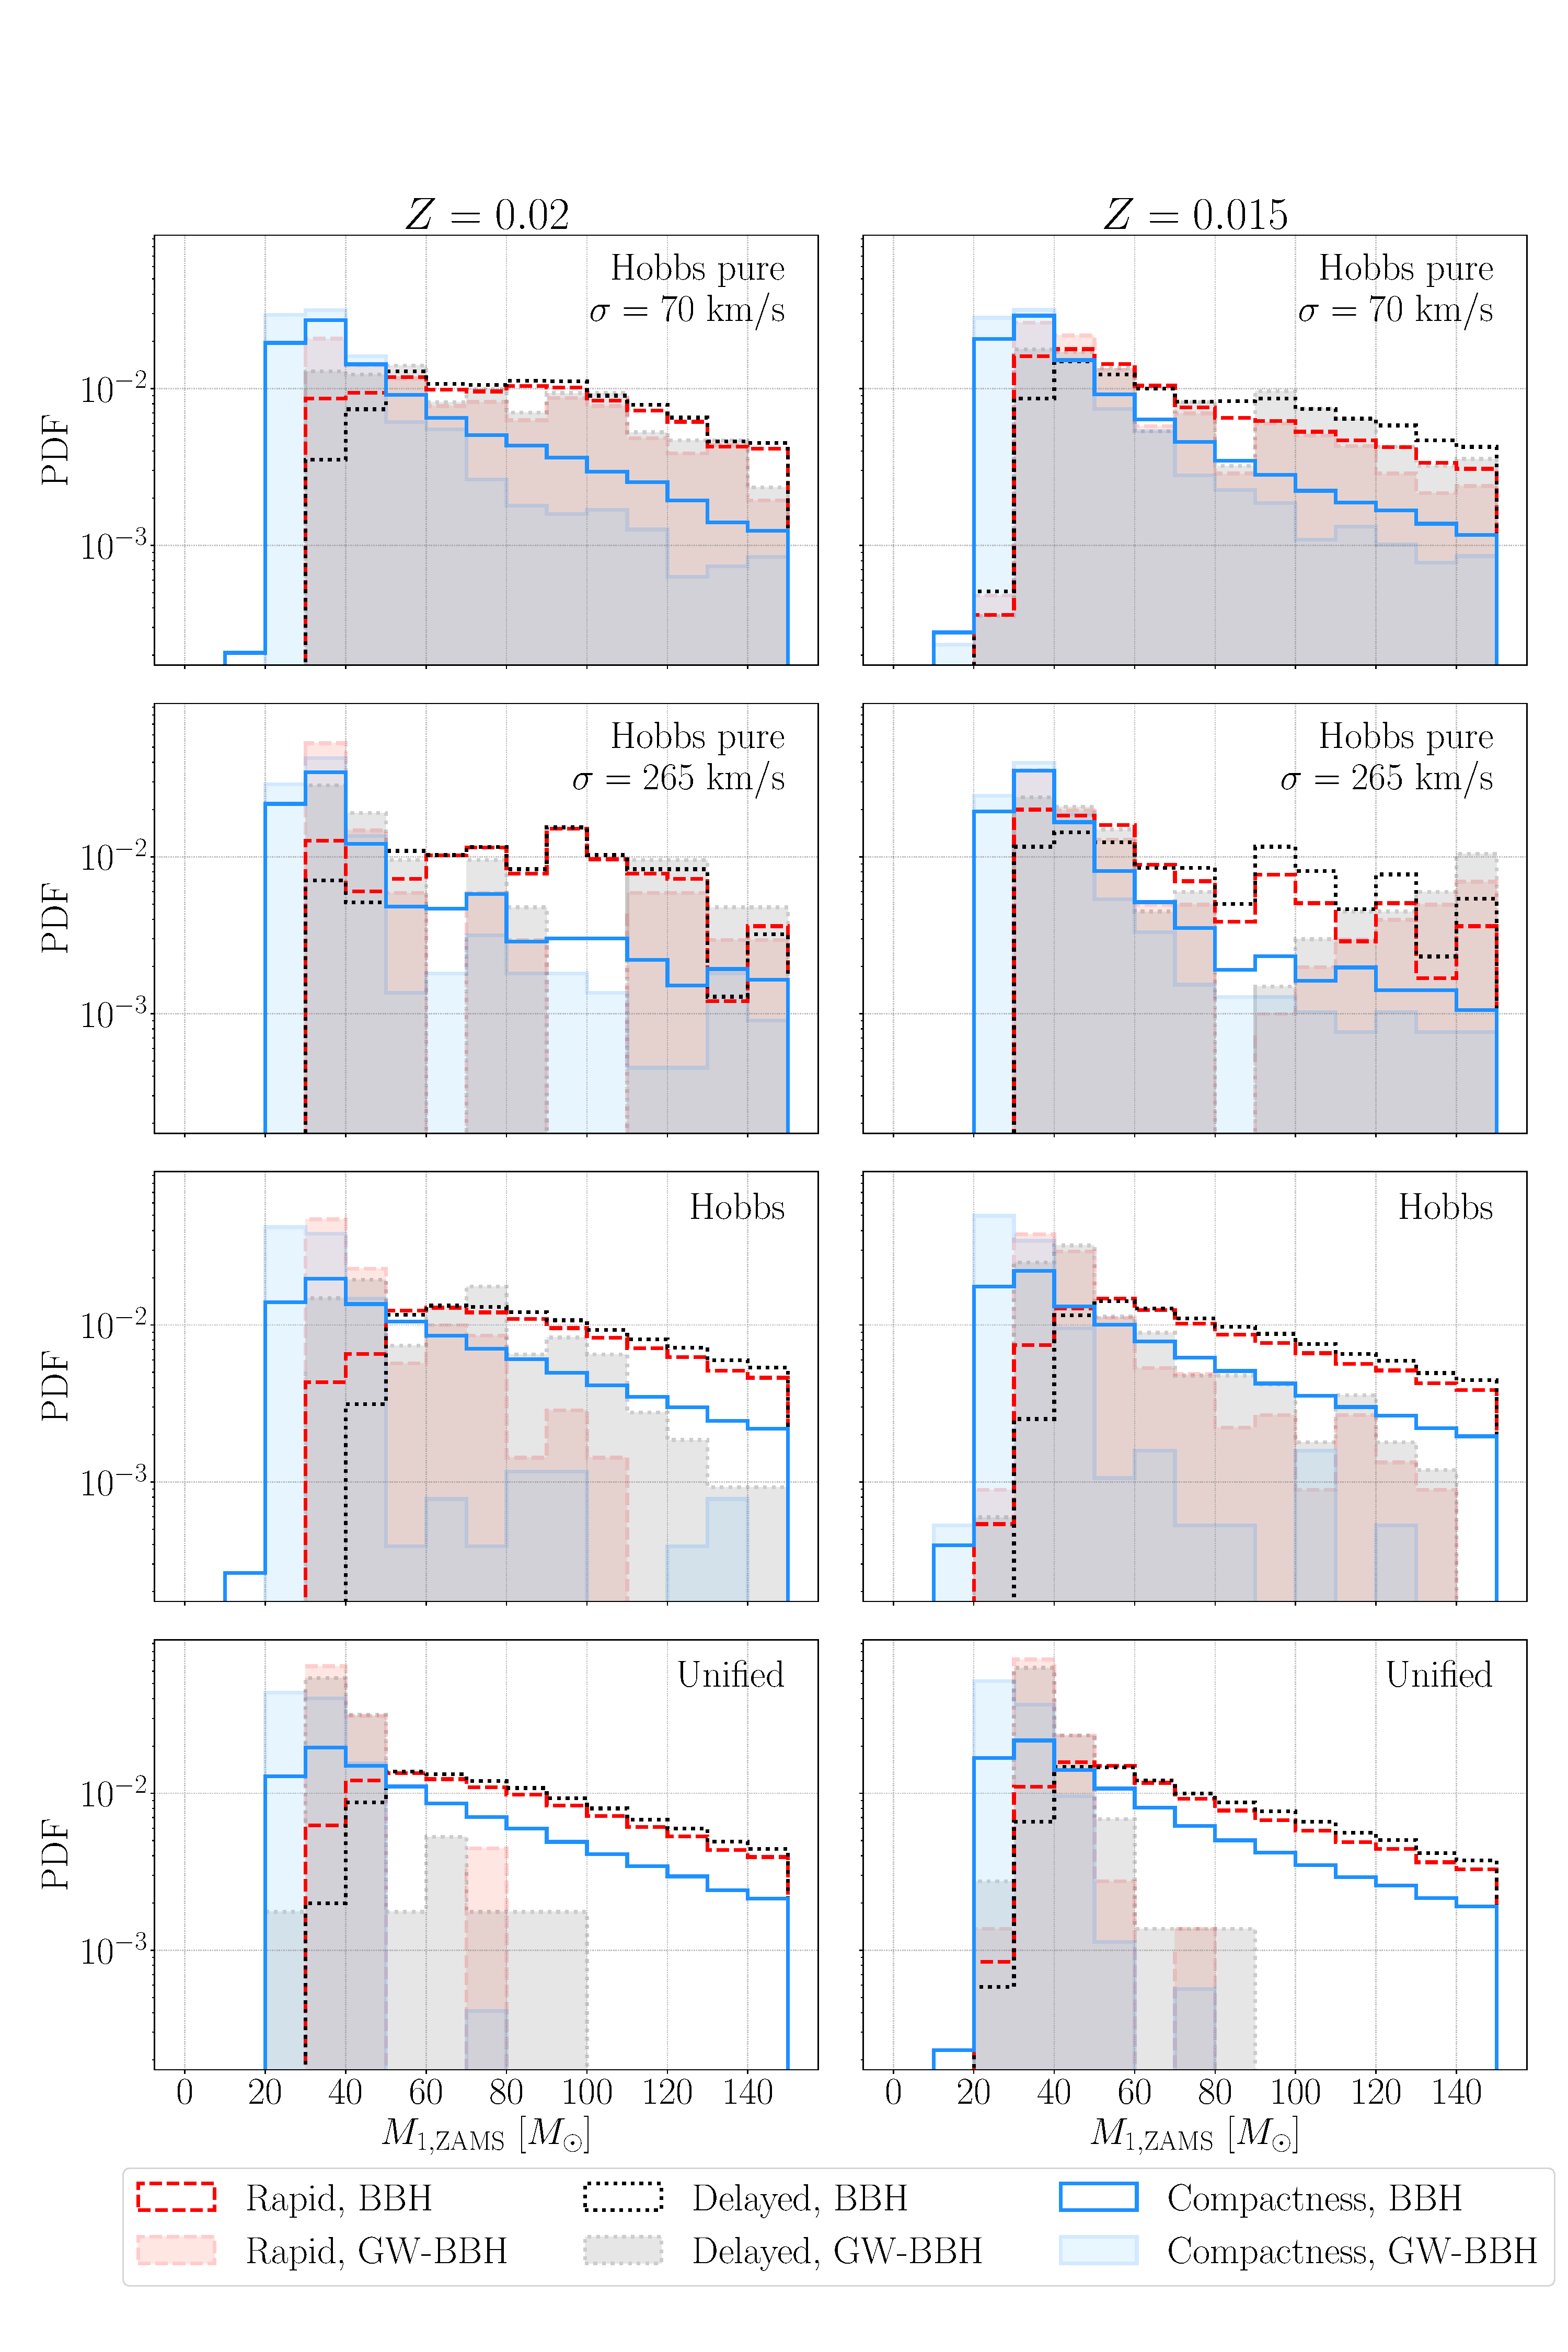
\includegraphics[width=\textwidth]{./images/progM1.pdf}	
	\caption{PDFs of primary masses $M_{\rm 1,ZAMS}$ at ZAMS for systems that will become BBHs (empty histograms) or GW--BBHs (filled histograms) after a WR--BH at $Z=0.02$ (\emph{left}) or $Z=0.015$ (\emph{right}) for different CCSN models (\emph{rapid}, red dashed line; \emph{delayed}, black dotted line; \emph{compactness}, blue solid line) and supernova kicks (from top to bottom: \emph{hobbs pure} with $\sigma = 70$ km/s or $\sigma = 265$ km/s; \emph{hobbs} or \emph{unified} with $\sigma = 265$ km/s).}\label{fig:resultsM1prog}
\end{figure}

\begin{figure}
	\centering
	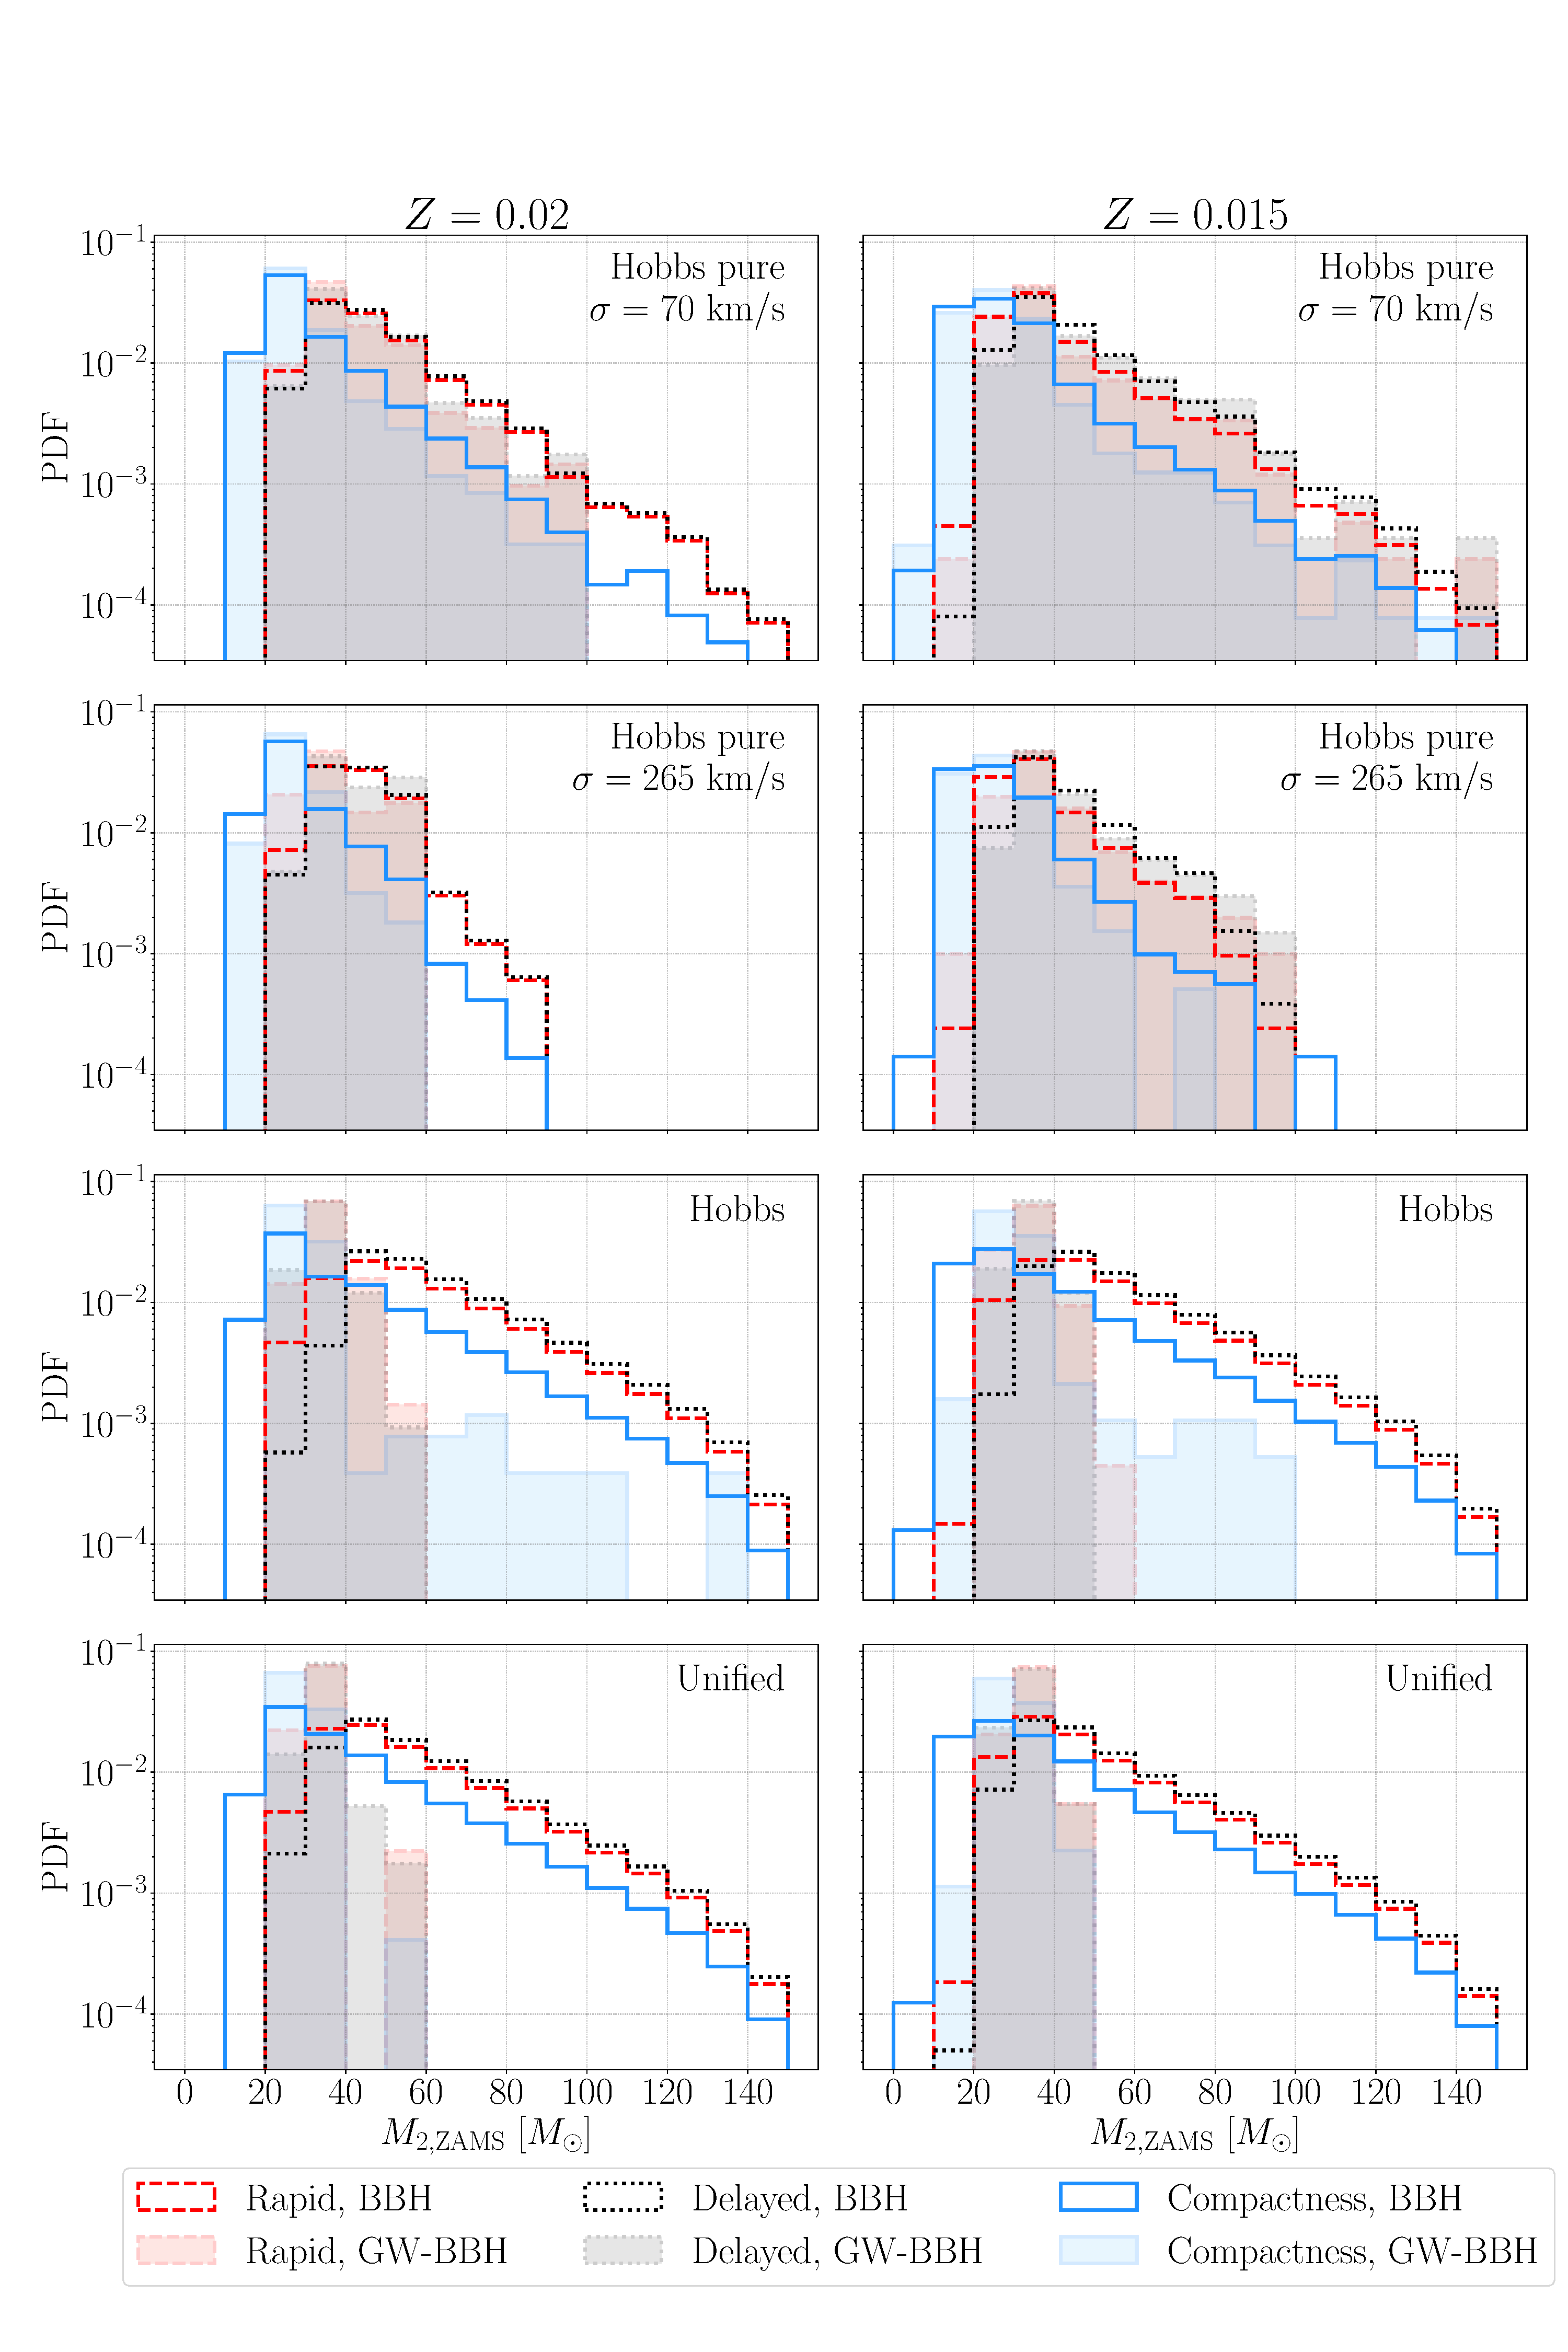
\includegraphics[width=\textwidth]{./images/progM2.pdf}	
	\caption{PDFs of secondary masses $M_{\rm 2,ZAMS}$ at ZAMS for systems that will become BBHs or GW--BBHs after a WR--BH for different metallicities $Z$, CCSN models and supernova kick options (see Fig.\ \ref{fig:resultsM1prog} for line-styles and colours).}\label{fig:resultsM2prog}
\end{figure}

\begin{figure}
	\centering
	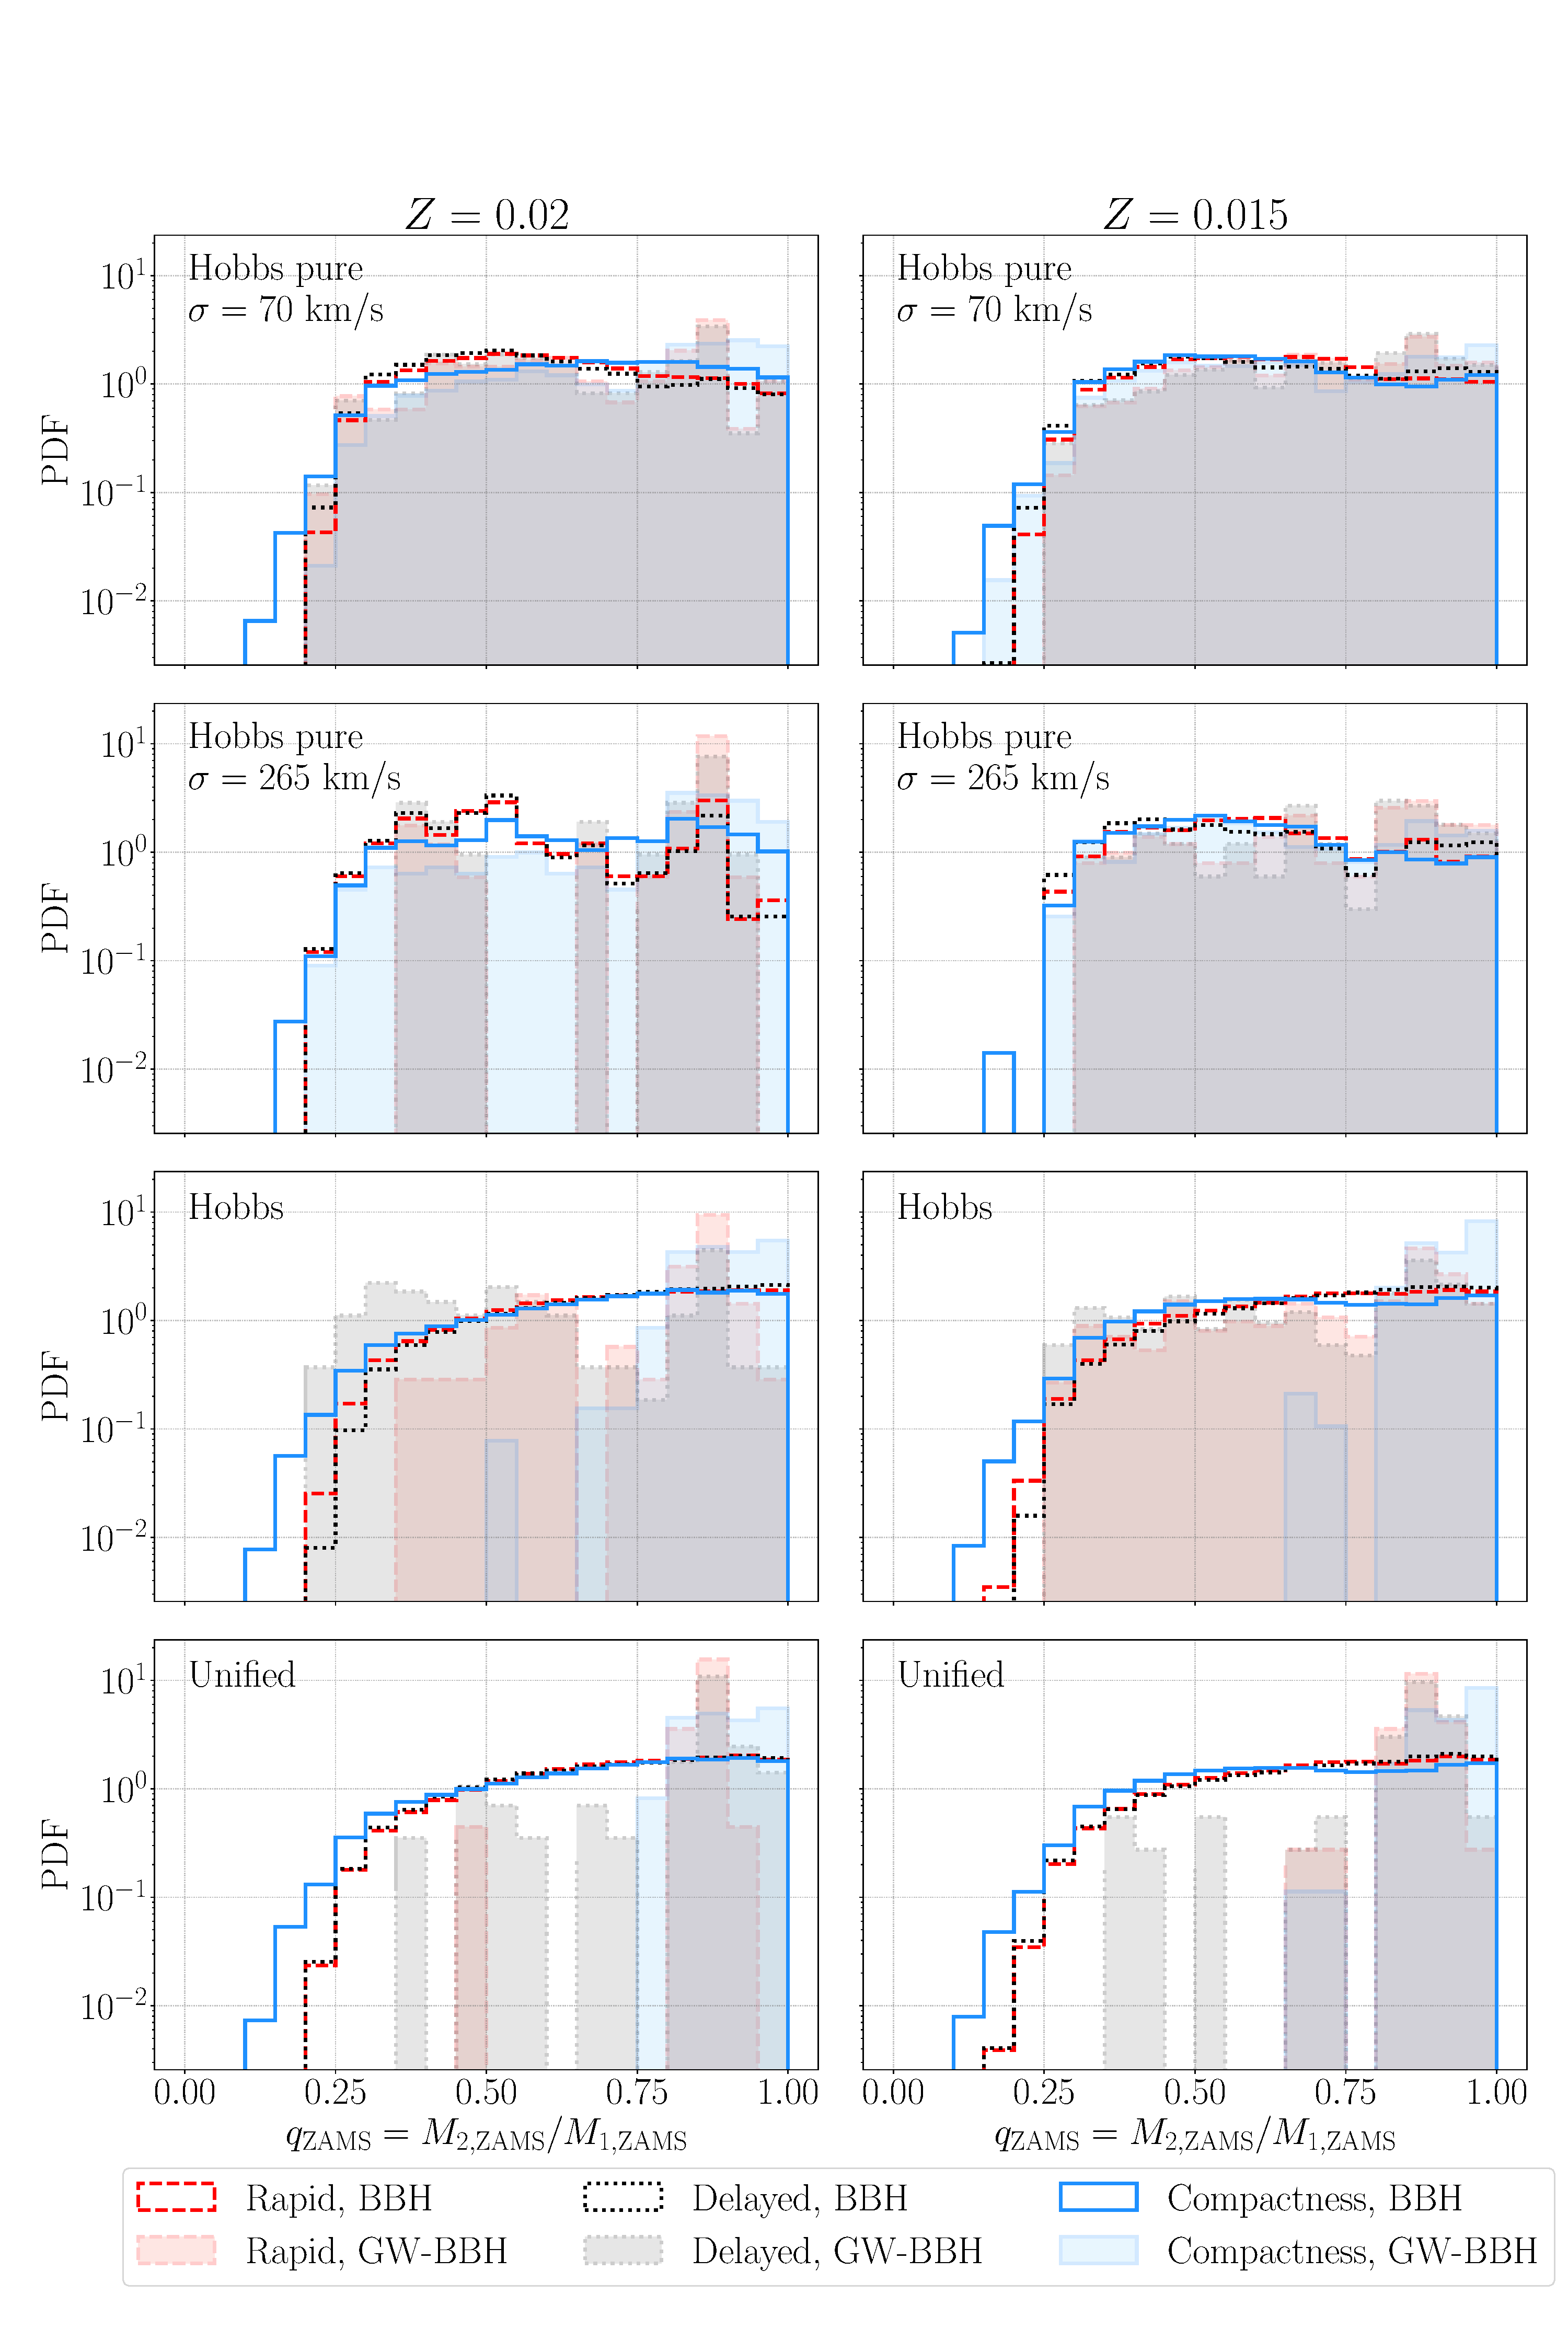
\includegraphics[width=\textwidth]{./images/progq.pdf}	
	\caption{PDFs of mass ratio $q_{\rm ZAMS}=M_{\rm 2,ZAMS}/M_{\rm 1,ZAMS}$ at ZAMS for systems that will become BBHs or GW--BBHs after a WR--BH for different metallicities $Z$, CCSN models and supernova kick options (see Fig.\ \ref{fig:resultsM1prog} for line-styles and colours).}\label{fig:resultsqprog}
\end{figure}

\begin{figure}
	\centering
	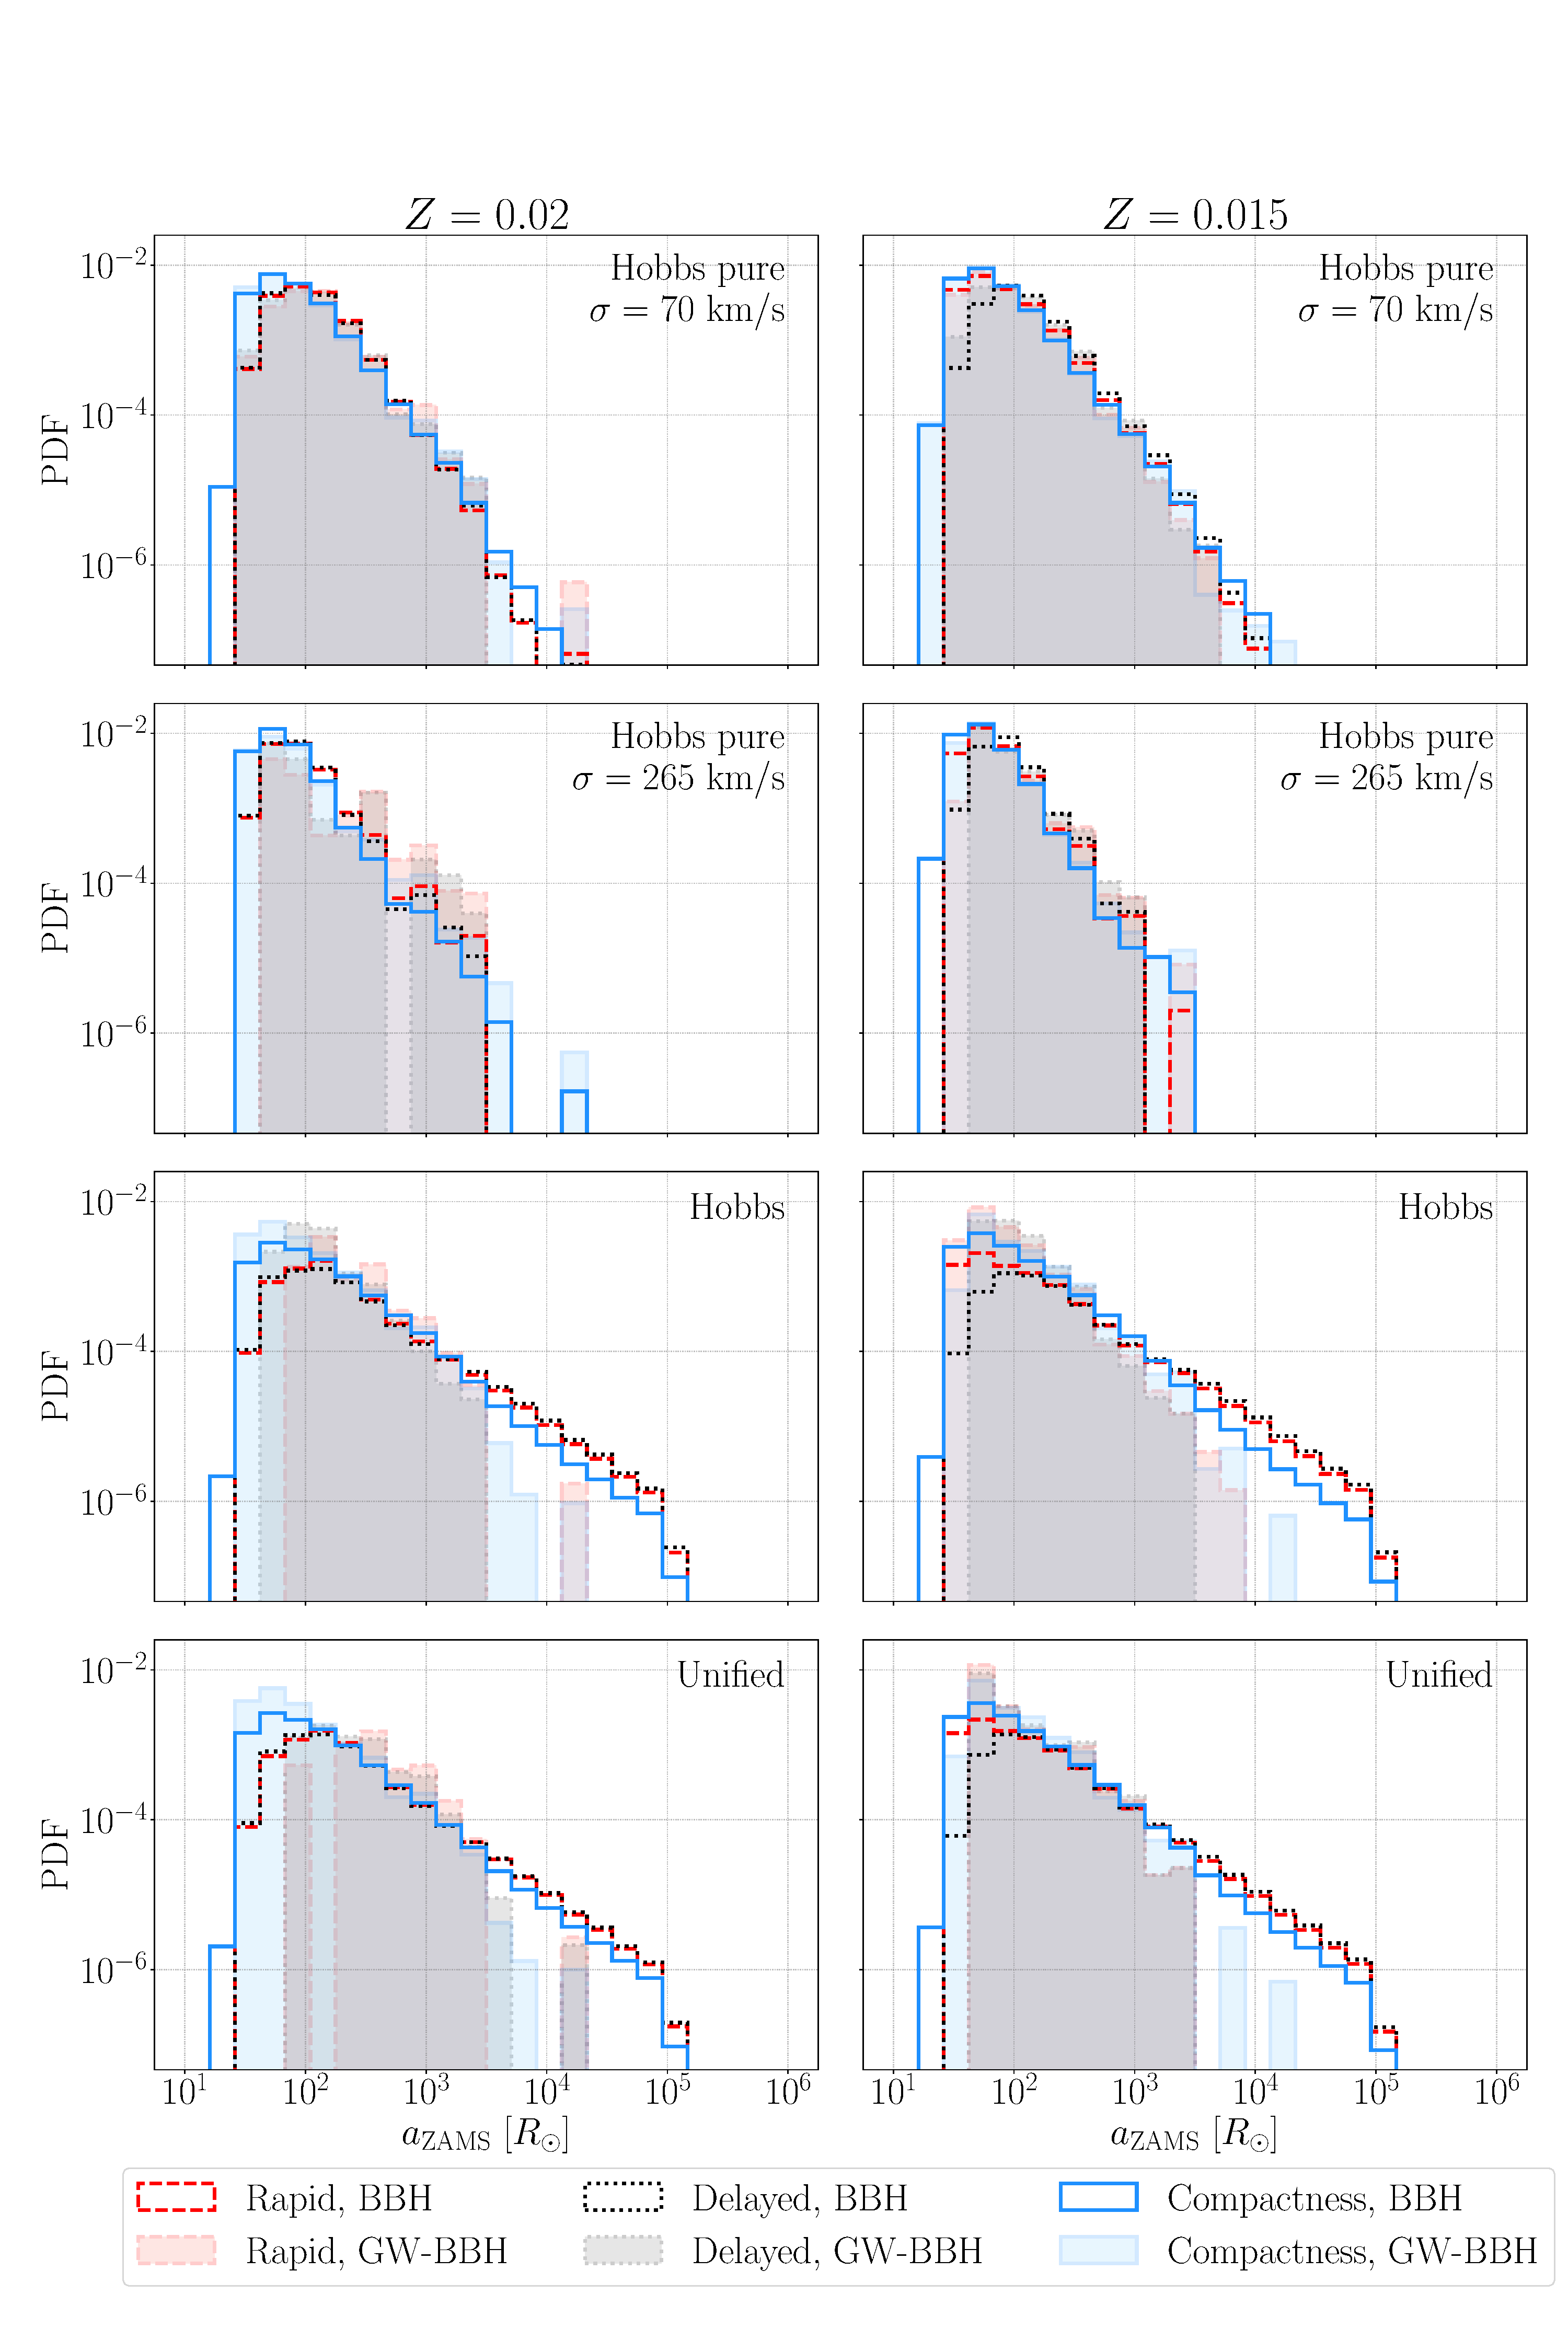
\includegraphics[width=\textwidth]{./images/proga.pdf}	
	\caption{PDFs of initial semi-major axis $a_{\rm ZAMS}$ at ZAMS for systems that will become BBHs or GW--BBHs after a WR--BH for different metallicities $Z$, CCSN models and supernova kick options (see Fig.\ \ref{fig:resultsM1prog} for line-styles and colours).}\label{fig:resultsaprog}
\end{figure}














\subsection{WR--BH phase}\label{subsec:WRBHphaseBBHsGWBBHs}
In this section, I will characterize WR--BH systems that are progenitors of BBHs and GW--BBHs by discussing their properties at the beginning of the WR--BH configuration. In some cases, I will discuss separately the evolution of systems where the Wolf-Rayet starts the WR--BH evolution with a H-rich envelope, thus is WN-like ($0 < H_{\rm sup} \leq 0.3$), or it is already a pure-helium star similar to WC and WO sub-types, hereafter collected under the shorter \emph{WCO} subscript (see Sec.\ \ref{subsec:stellarevo} and \ref{subsec:stellarphasesSEVN} for more detailed information on the Wolf-Rayet star classification adopted in this thesis).


\paragraph{Black hole masses} Fig.\ \ref{fig:resultsWRBH-MBH} shows the PDFs of black holes at the beginning of the WR--BH phase. The mass of the lightest black holes depends on the CCSN model adopted, as already discussed in Sec.\ \ref{subsec:SNmodels}: the \emph{rapid} model does not allow $\mbh < 5~\msun$ while the \emph{delayed} and \emph{compactness} options form black holes down to the $3~\msun$ threshold, set to distinguish neutron stars from black holes. In contrast, metallicity affects the maximum black hole mass because less metallic stars have less efficient stellar winds, thus, are able to retain more mass. \\

For all supernova kick and CCSN models, the maximum black hole mass for BBHs is well-defined and is only affected by the metallicity, being $M_{\rm BH,max} \sim 25~\msun$ at $Z=0.02$ and $M_{\rm BH,max} \sim 35~\msun$ at $Z=0.015$. While the PDFs for BBH progenitors are all alike, the ones for GW--BBH progenitors indicate that some combinations of the parameter space slightly favour different black hole masses. In particular, PDFs for GW--BBHs progenitors reduce the maximum black hole mass in the WR--BH phase of $\sim 5~\msun$ for both metallicities. Moreover, systems evolved with the \emph{compactness} CCSN model are less likely to form primary black holes with mass $\sim 10-15~\msun$ ($\sim 15-20~\msun$) for $Z=0.02$ ($Z=0.015$) and, if evolved with the \emph{unified} kick model, completely lack black holes above these thresholds.

In general, the production of black holes $\lesssim 35~\msun$ is reasonable at solar metallicity, where the effect of stellar winds is still relevant (see Fig.\ \ref{fig:masslostWR} for a comparison with $Z=0.002$). The slightly lighter black holes found in systems that will merge via gravitational wave emission within a Hubble time may indicate that similar systems evolved in tighter orbits and that their progenitor stars underwent at least a mass transfer episode as donor. For instance, the discussion carried out in Sec.\ \ref{sec:resultsCygX3evo} will confirm that this is the case at least for binaries like Cyg X-3.






\paragraph{Two WR--BHs families for WN and WCO Wolf-Rayet stars} Figures~\ref{fig:resultsWRBH-MWRnonpureHe}, \ref{fig:resultsWRBH-anonpureHe} and \ref{fig:resultsWRBH-RLfillnonpureHe} show mass $M_{\rm WN}$, semi-major axis $a_{\rm WN-BH}$ and Roche lobe filling fraction $R_{\rm WN}/R_{\rm L,WN}$, respectively, for WR--BH systems born with a H-rich Wolf-Rayet star that is WN-like. These stars are not yet modelled as pure-helium and are a mixture of H-core, H-shell and He-core burning stars (\texttt{BSE} phases = 1, 2, 3, 4 according to the classification explained in Sec.\ \ref{subsec:stellarphasesSEVN}). Similarly, Fig.\ \ref{fig:resultsWRBH-MWRpureHe}, \ref{fig:resultsWRBH-apureHe} and \ref{fig:resultsWRBH-RLfillpureHe} show mass $M_{\rm WCO}$, semi-major axis $a_{\rm WCO-BH}$ and Roche lobe filling fraction $R_{\rm WCO}/R_{\rm L,WCO}$ for WR--BH systems born with WC- and WO-like Wolf-Rayet stars, modelled with pure-helium tracks.\\



WN-like stars in BBH progenitors are distributed among a wide range of masses $M_{\rm WN} \sim 8-60~\msun$, with a different lower minimum cutoff at $\sim 25~\msun$ only for the model with the stronger kicks (\emph{hobbs pure} with a $\sigma=265$ km/s Maxwellian root-mean-square). In contrast, WC- and WO-like stars in BBH progenitors are always lighter than $M_{\rm WCO} \lesssim 30-40~\msun$, also reaching lower minimum masses of $\sim 5~\msun$. Even though the WN $\rightarrow$ WCO evolution (see Sec.\ \ref{subsec:WRclassification}) could, in part, explain the lighter WCO stars, the mass difference seems to be correlated also with other binary properties.

For instance, there are no BBH progenitors with a WN-like Wolf-Rayet star with a WN--BH orbit tighter than $a_{\rm min, WN-BH} \sim 50-100~\rsun$, whereas BBH progenitors with a pure-helium star form also with semi-major axis comparable to Wolf-Rayet star radii $a_{\rm min, WCO-BH} \sim 1~\rsun$. The very close orbits of WCO--BH systems coupled with the fact that WCO Wolf-Rayet stars lack an hydrogen envelope suggest that their WR--BH configuration has been reached at least after one common envelope. In contrast, it is likely that WN--BH binaries did not form after a common envelope evolution because most of their donors lack a prominent He core (see Sec.\ \ref{subsec:masstransferSEVN}).\\

Many WN-like stars considered here exhibit Roche lobe filling fractions well-beyond $R_{\rm WN}/R_{\rm L,WN} > 1$, suggesting that they are losing their hydrogen envelope as a consequence of a stable Roche lobe overflow\footnote{Roche lobe overflow routines in \texttt{SEVN} use the stellar radius only for stellar wind calculations. The radius adopted in Fig.\ \ref{fig:resultsWRBH-RLfillnonpureHe} and \ref{fig:resultsWRBH-RLfillpureHe} is not physical and is only a proxy for systems with active Roche lobe overflows (see Sec.\ \ref{subsec:masstransferSEVN}).}. In contrast, WC- and WO-like Wolf-Rayet stars are more compact and are less likely to start the WR--BH evolution with a Roche lobe overflow. Nevertheless, the PDFs shown in Fig.\ \ref{fig:resultsWRBH-RLfillnonpureHe} and \ref{fig:resultsWRBH-RLfillpureHe} indicate that the majority of all Wolf-Rayet stars considered here is not overfilling its Roche lobe: at most, they are powering a wind-fed accretion.



\paragraph{WN--BHs as GW--BBHs progenitors only with final eccentricity $\boldsymbol{e_{\rm BBH} \sim 1}$} A similar discussion can be carried out also for WR--BH systems that are GW--BBH progenitors: their PDFs follow closely the distribution of BBH progenitors, with two major differences. The first relevant one highlights the need for relatively tight orbits to allow the merger via gravitational-wave emission within a Hubble time: only WR--BH systems born with $a_{\rm WR-BH} \lesssim 10^3$~R$_\odot$ are likely to merge (Figures~\ref{fig:resultsWRBH-anonpureHe} and \ref{fig:resultsWRBH-apureHe}). Wider or similar binaries require either a large eccentricity (see Fig.\ \ref{fig:resultsRemEccentricity}) or massive black holes in order to shorten the time required to merge, as indicated by Eq.\ \ref{eq:tgw}. 


Such restrictive conditions determine the second difference in the PDFs: almost none of the systems born with WN-like Wolf-Rayet stars is a GW--BBH progenitor if it is evolved with supernova kicks re-scaled for fallback (\emph{hobbs} model) or compact object and ejecta masses (\emph{unified} model).\\

As shown in Fig.\ \ref{fig:resultsWRBH-anonpureHe}, WR--BH systems born with a WN-like star produce a BBH only if they have initial semi-major axis $a_{\rm WN-BH} \gtrsim 50-100 ~ \rsun$, thus becoming GW--BBHs only if at the beginning of the WN--BH phase have $a_{\rm WN-BH} \sim 10^2 - 10^3 ~ \rsun$. As anticipated, only massive systems will merge within a Hubble time from similarly large semi-major axis: in fact, only WN--BH binaries born with $M_{\rm BH} \sim 10-30~\msun$ and $M_{\rm WN} \sim 15-50~\msun$ will produce GW--BBHs. However, hosting massive objects is not sufficient to shorten the time required to merge via gravitational wave emission from orbits so wide: all the simulated WN--BH systems that become GW--BBHs have $e_{\rm BBH} \sim 1$. 

The need for highly eccentric orbits is even more evident in systems evolved with damped kicks: WN--BH binaries are the only systems in the $e_{\rm BBH} \sim 1$ bin of Fig.\ \ref{fig:resultsRemEccentricity} for GW--BBHs for the \emph{unified} model with \emph{rapid} CCSN at $Z=0.02$ and \emph{hobbs} model with \emph{compactness} CCSN at both metallicities. Following Sec.\ \ref{subsec:SEVNpostsupernovaorbit}, high-velocity kicks can be randomly projected into a wide range of orbital velocities and are more likely to ionize the binary or produce high eccentric post-supernova orbits, explaining the larger number of WN--BH binaries that could become GW--BBH when evolved with the \emph{hobbs pure} option. 

In contrast, WC- and WO-like Wolf-Rayet stars with a black hole companion are allowed to form in tighter orbits, thus, are less affected by supernova kicks. Systems born with semi-major axis down to $a_{\rm WCO-BH} \sim 1~\rsun$ are more likely to produce GW--BBHs, therefore they extend the range of the possible progenitors to lower masses: $M_{\rm BH} \gtrsim 3~\msun$ and $M_{\rm WCO} \gtrsim 5~\msun$.


\paragraph{Observability in the WR--BH configurations}
WR--BH binaries that are BBH and GW--BBH progenitors evolve for $\sim 2.5 - 15$ Myr before reaching the WR--BH configuration. As shown in Fig.\ \ref{fig:resultsWRBH-time}, there is not a well-defined duration for the WR--BH phase of BBH progenitors: they could last from $\sim 10$ years to $\sim 1$ Myr. Only binaries evolved with the stronger kicks (\emph{hobbs pure} option with $\sigma=265$ km/s) spend at least $\gtrsim 5 \times 10^3$ years in the WR--BH configuration. This is also the minimum duration required to become GW--BBHs from the WR--BHs phase and is a lower boundary common to all the simulated sets, further indicating that the few black holes to survive in a bound orbit in the \emph{hobbs pure} option with $\sigma=265$ km/s occupy the same parameter space of GW-BBH progenitors.

As shown in Fig.\ \ref{fig:resultsWRBH-P}, GW-BBH progenitors that are visible as WR--BHs for $\sim 5 \times 10^3 - 10^6$ years have initial orbital periods of $\sim 1~\text{hour} - 10~\text{years}$. In particular, WCO--BH binaries exhibit bimodal period distributions similar to the ones of Fig.\ \ref{fig:resultsWRBH-P}, with preference for systems with initial periods of few hours or few months. In contrast, WN--BH binaries are limited by the wide orbits to have periods $\gtrsim 10^{-1}$ years, enhancing the peak at higher periods.\\

Overall, this work suggests that WR--BH binaries with orbital periods $\lesssim 10$ years could be GW--BBH progenitors, with higher probability for WR--BHs with periods shorter than a few days but not shorter than about one hour (otherwise the binary would collide and merge prematurely). This further supports the discussion carried out in Sec.\ \ref{sec:WRBHobserved}. In fact, six out of the seven WR--BH observed candidates have periods of $\sim 5-35$ hours and will likely become GW--BBH progenitors. Instead, the fate of M101 ULX-1 remains uncertain because it has a period of $\sim 8$ days that falls in a region where being a GW--BBH progenitor depends on the kick model adopted: the \emph{hobbs pure} model allows it while kicks damped with \emph{hobbs} and \emph{unified} options avoid a similar fate.

\clearpage






\begin{figure}[h!]
	\centering
	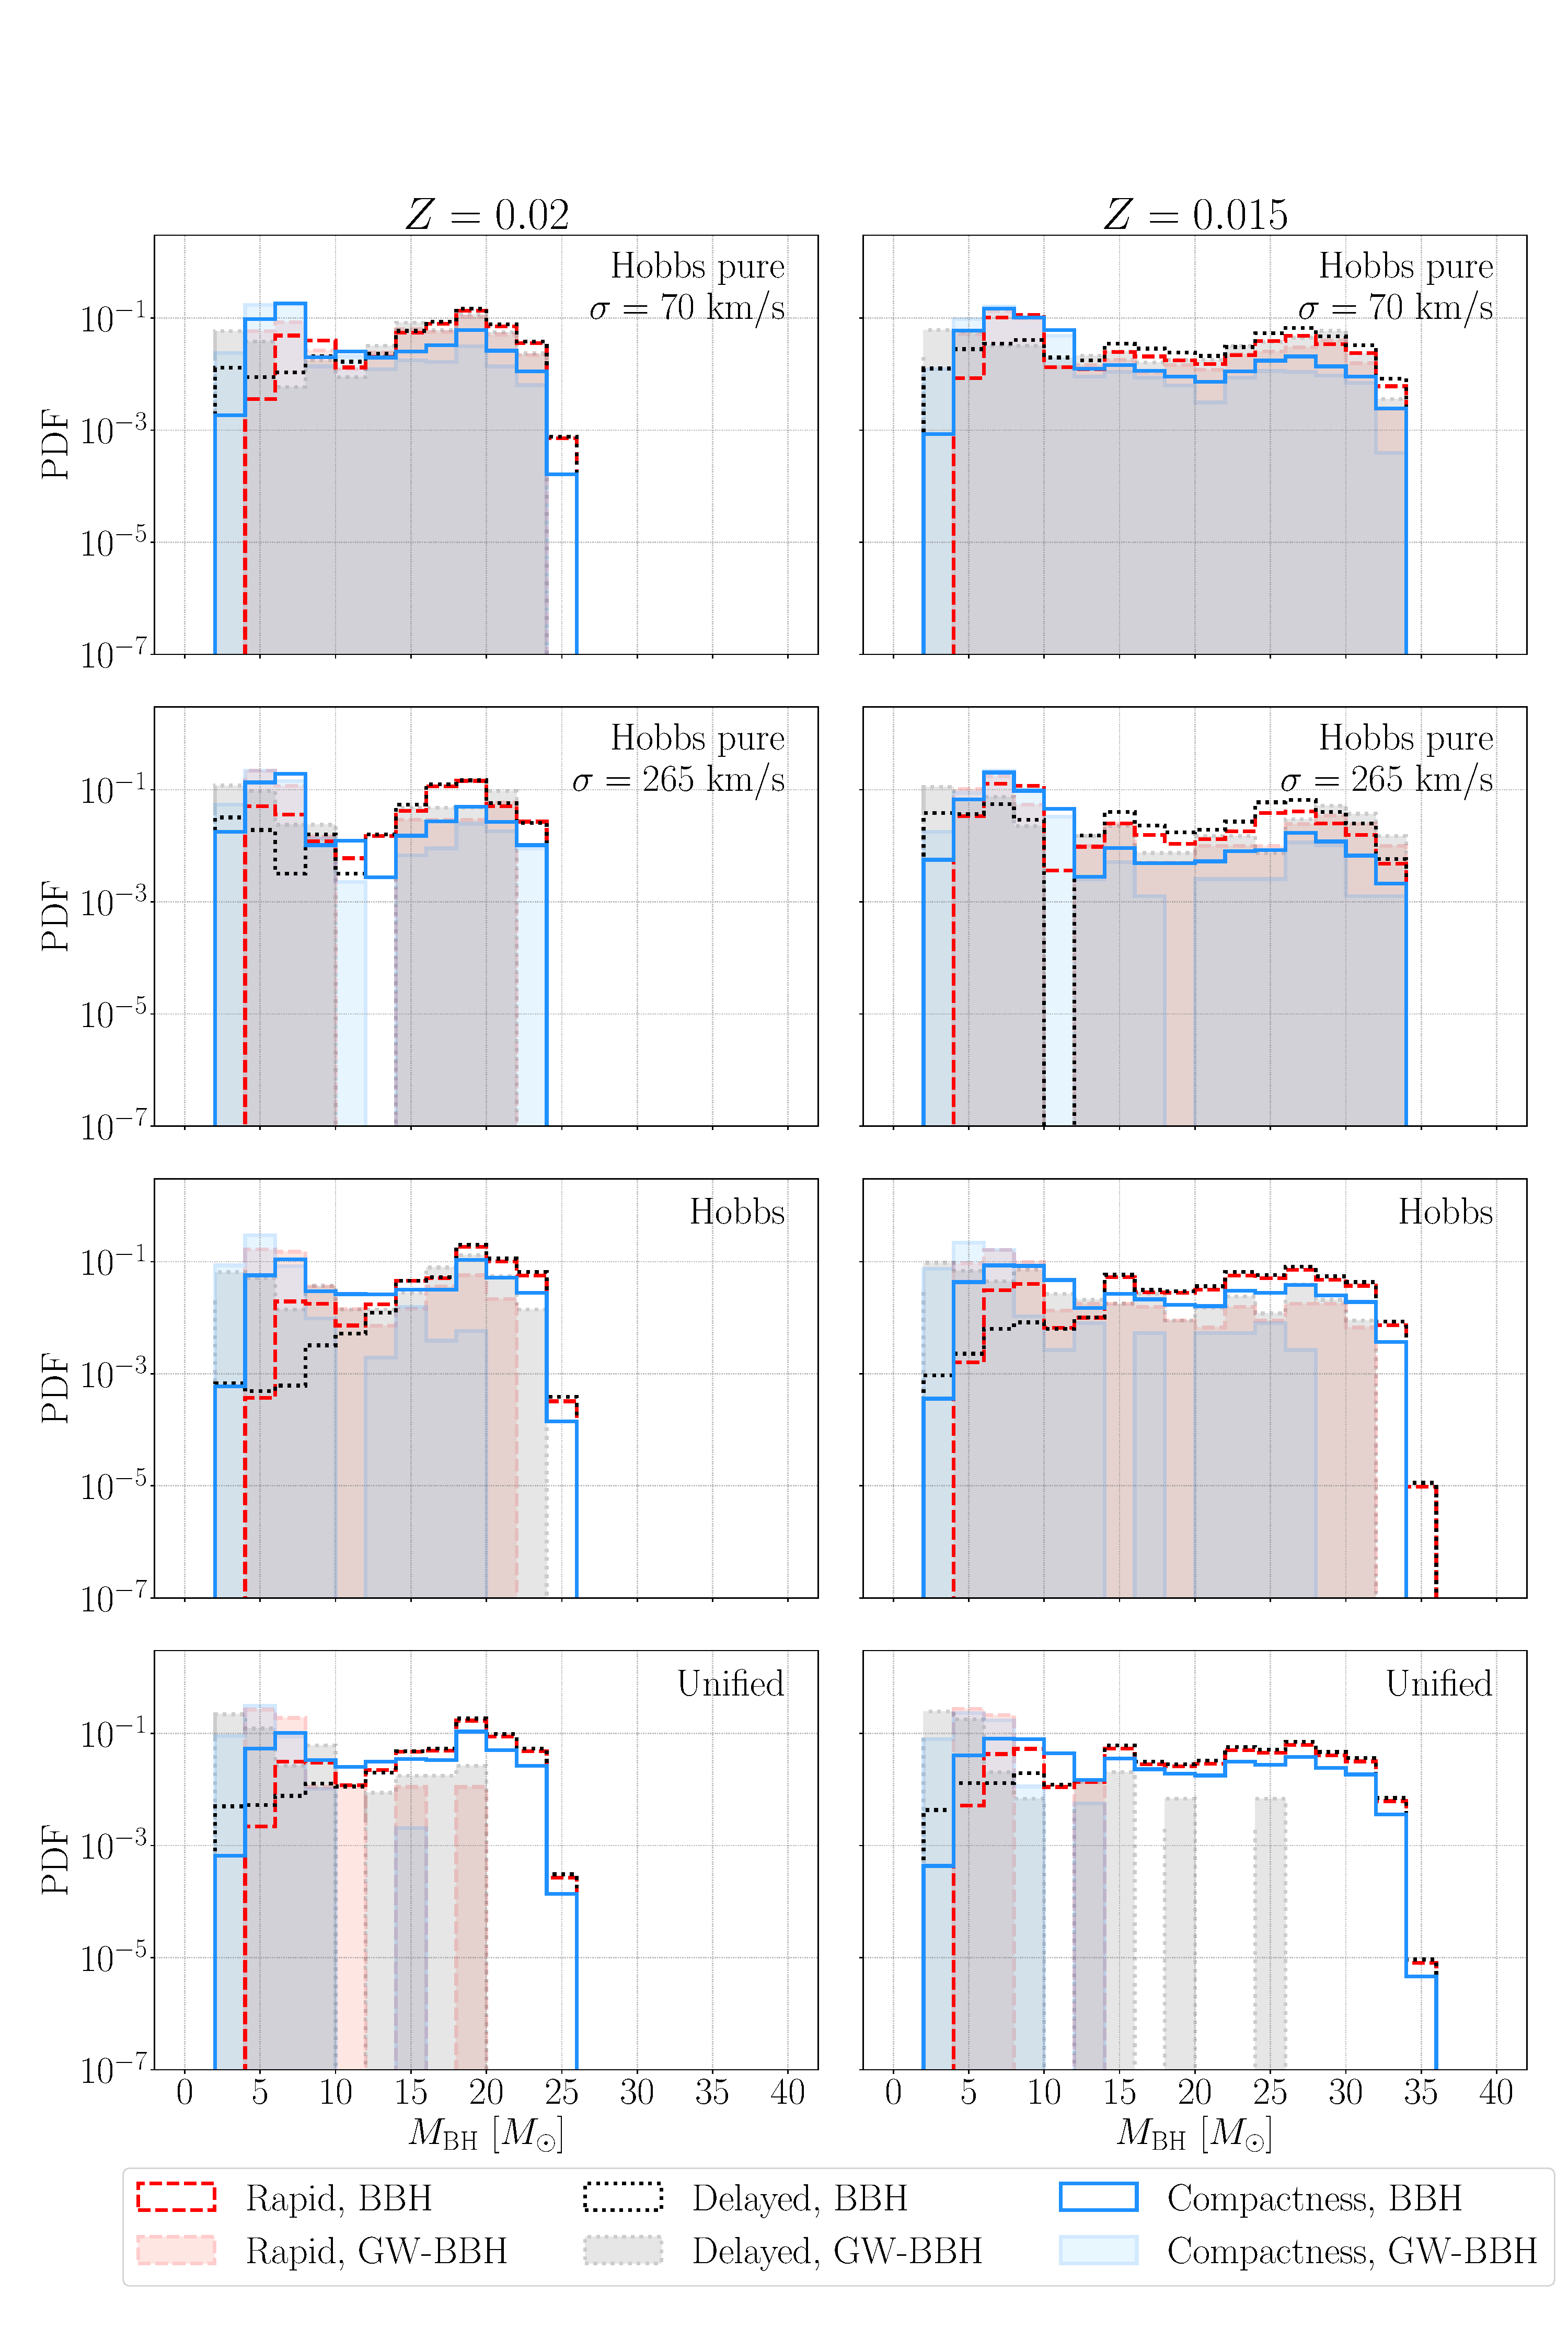
\includegraphics[width=\textwidth]{./images/WRBH-MBH.pdf}	
	\caption{PDFs of black hole mass $M_{\rm BH}$ at the beginning of the WR--BH phase for systems that will become BBHs or GW--BBHs after a WR--BH for different metallicities $Z$, CCSN models and supernova kick options (see Fig.\ \ref{fig:resultsM1prog} for line-styles and colours).}\label{fig:resultsWRBH-MBH}
\end{figure}


\begin{figure}[h!]
	\centering
	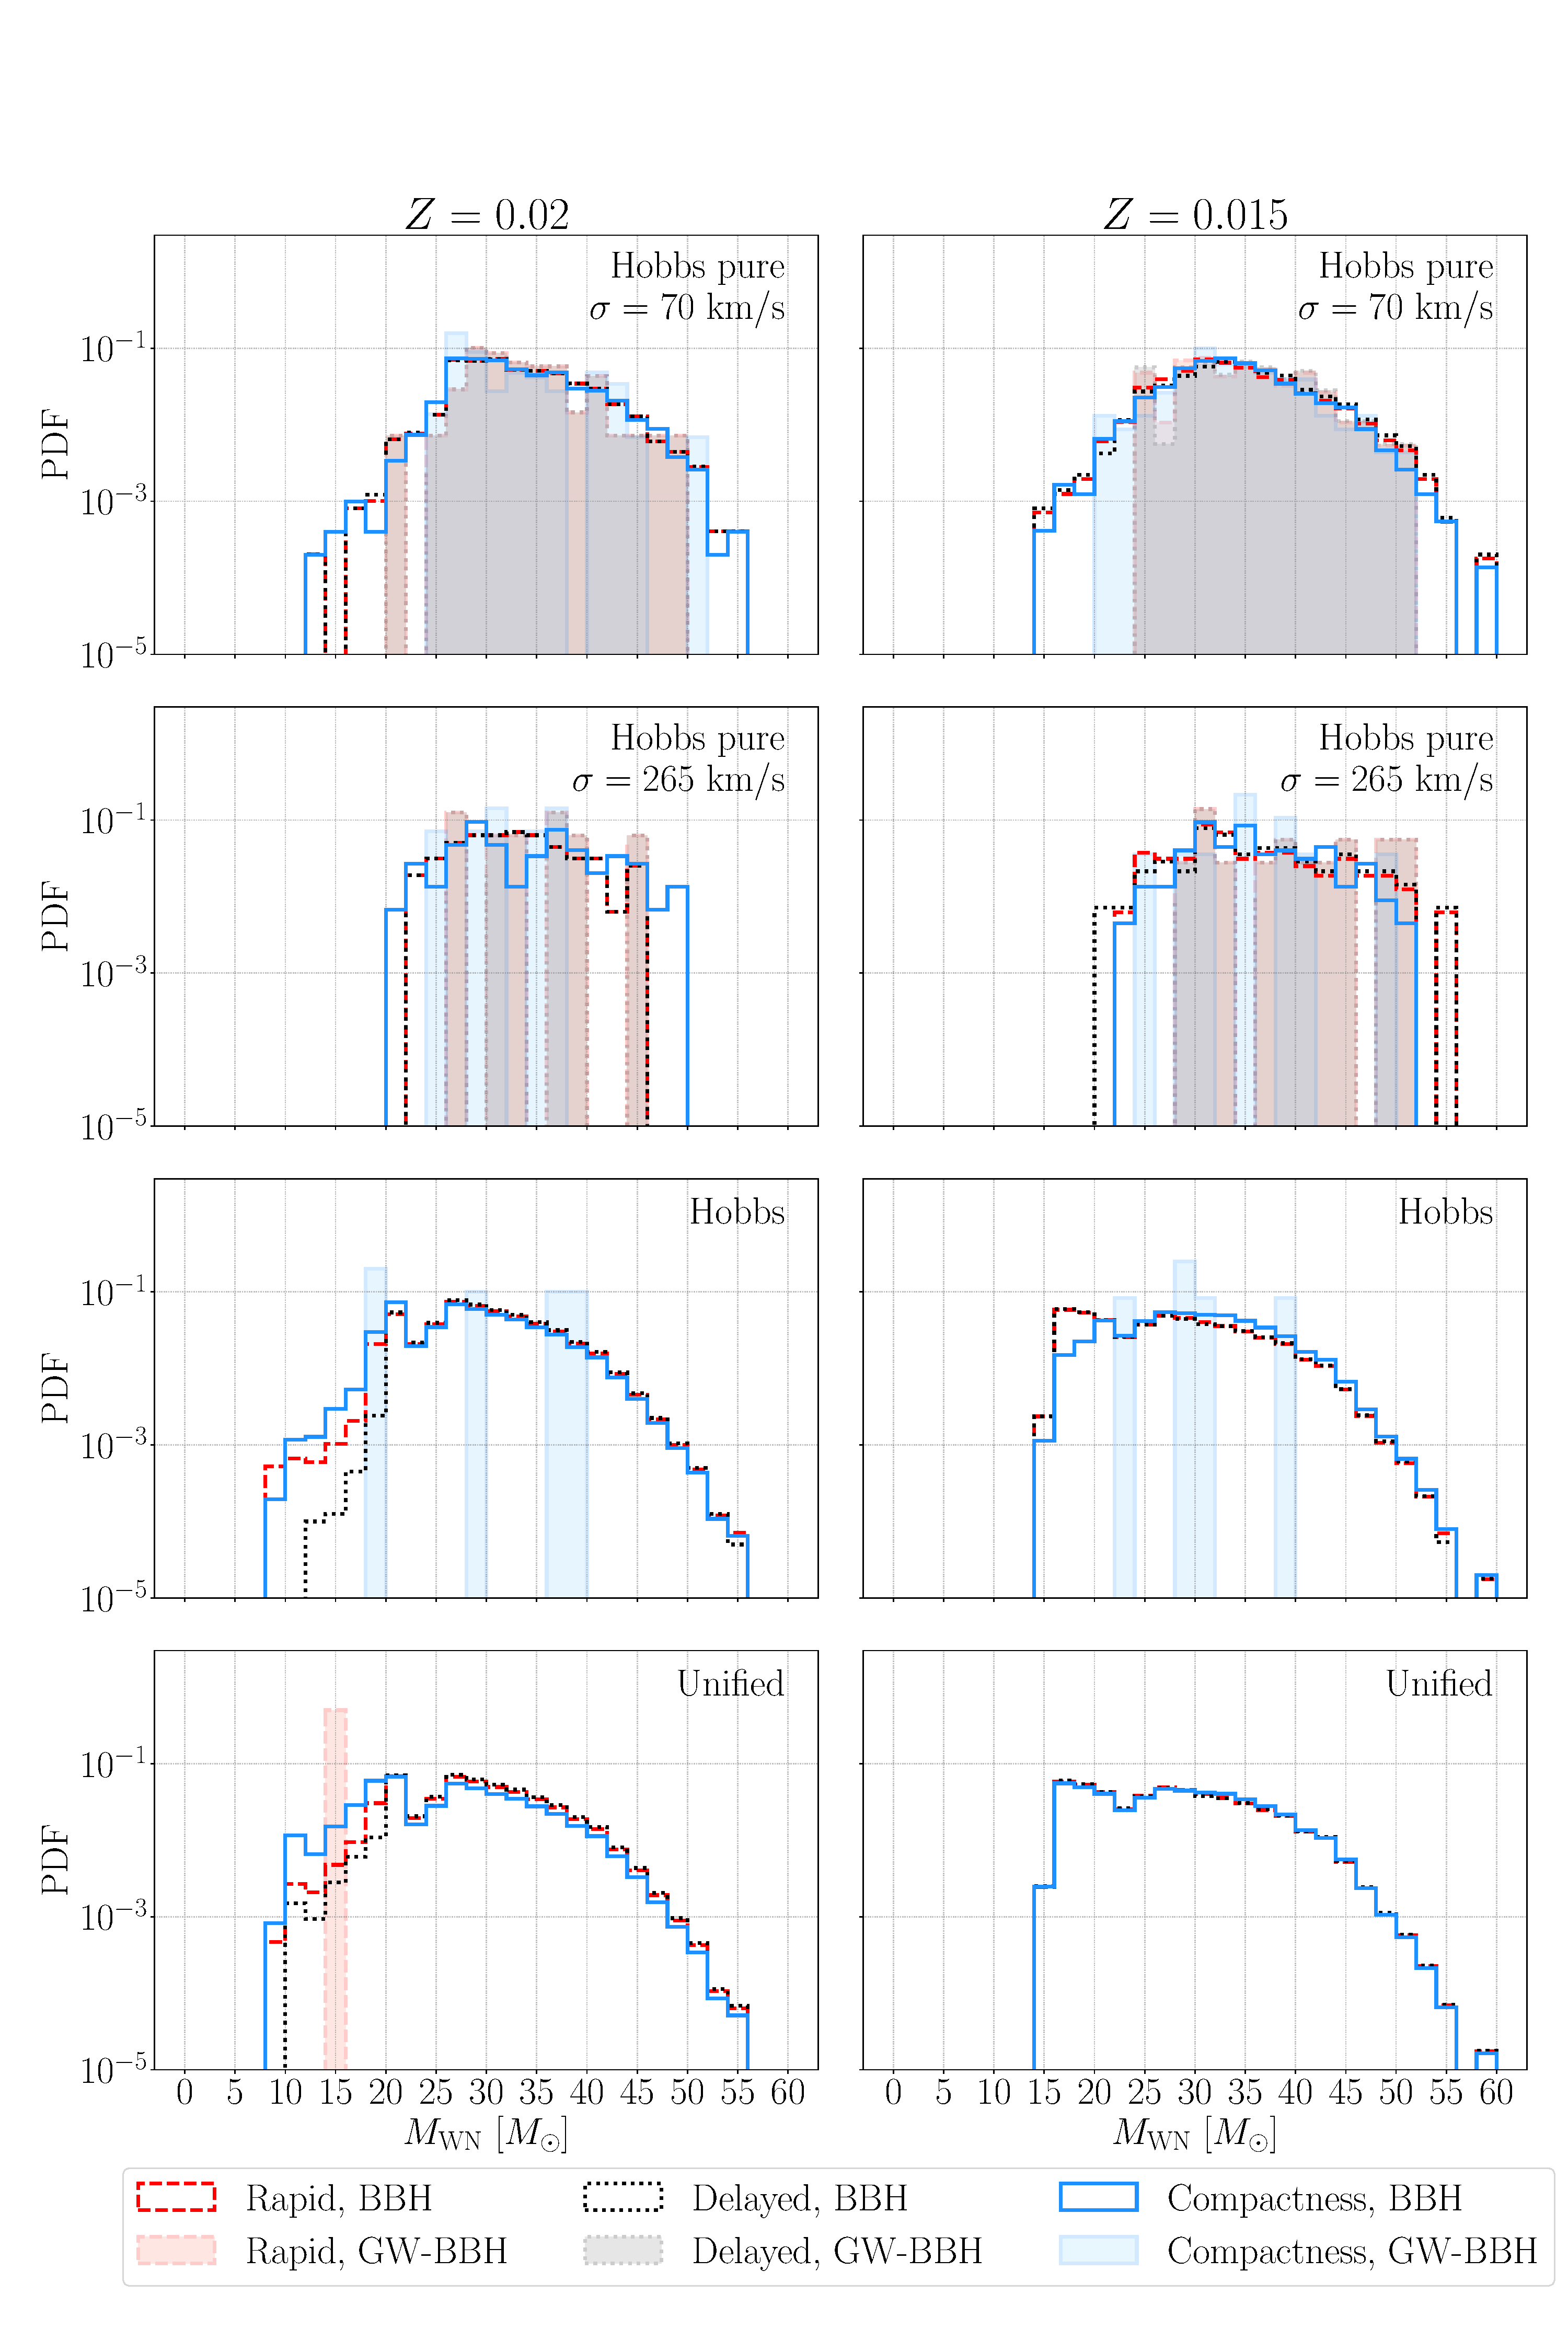
\includegraphics[width=\textwidth]{./images/WRBH-MWRnonpureHe.pdf}	
	\caption{PDFs of masses of Wolf-Rayet WN-like stars $M_{\rm WN}$ at the beginning of the WR--BH phase for systems that will become BBHs or GW--BBHs after a WR--BH for different metallicities $Z$, CCSN models and supernova kick options (see Fig.\ \ref{fig:resultsM1prog} for line-styles and colours).}\label{fig:resultsWRBH-MWRnonpureHe}
\end{figure}


\begin{figure}[h!]
	\centering
	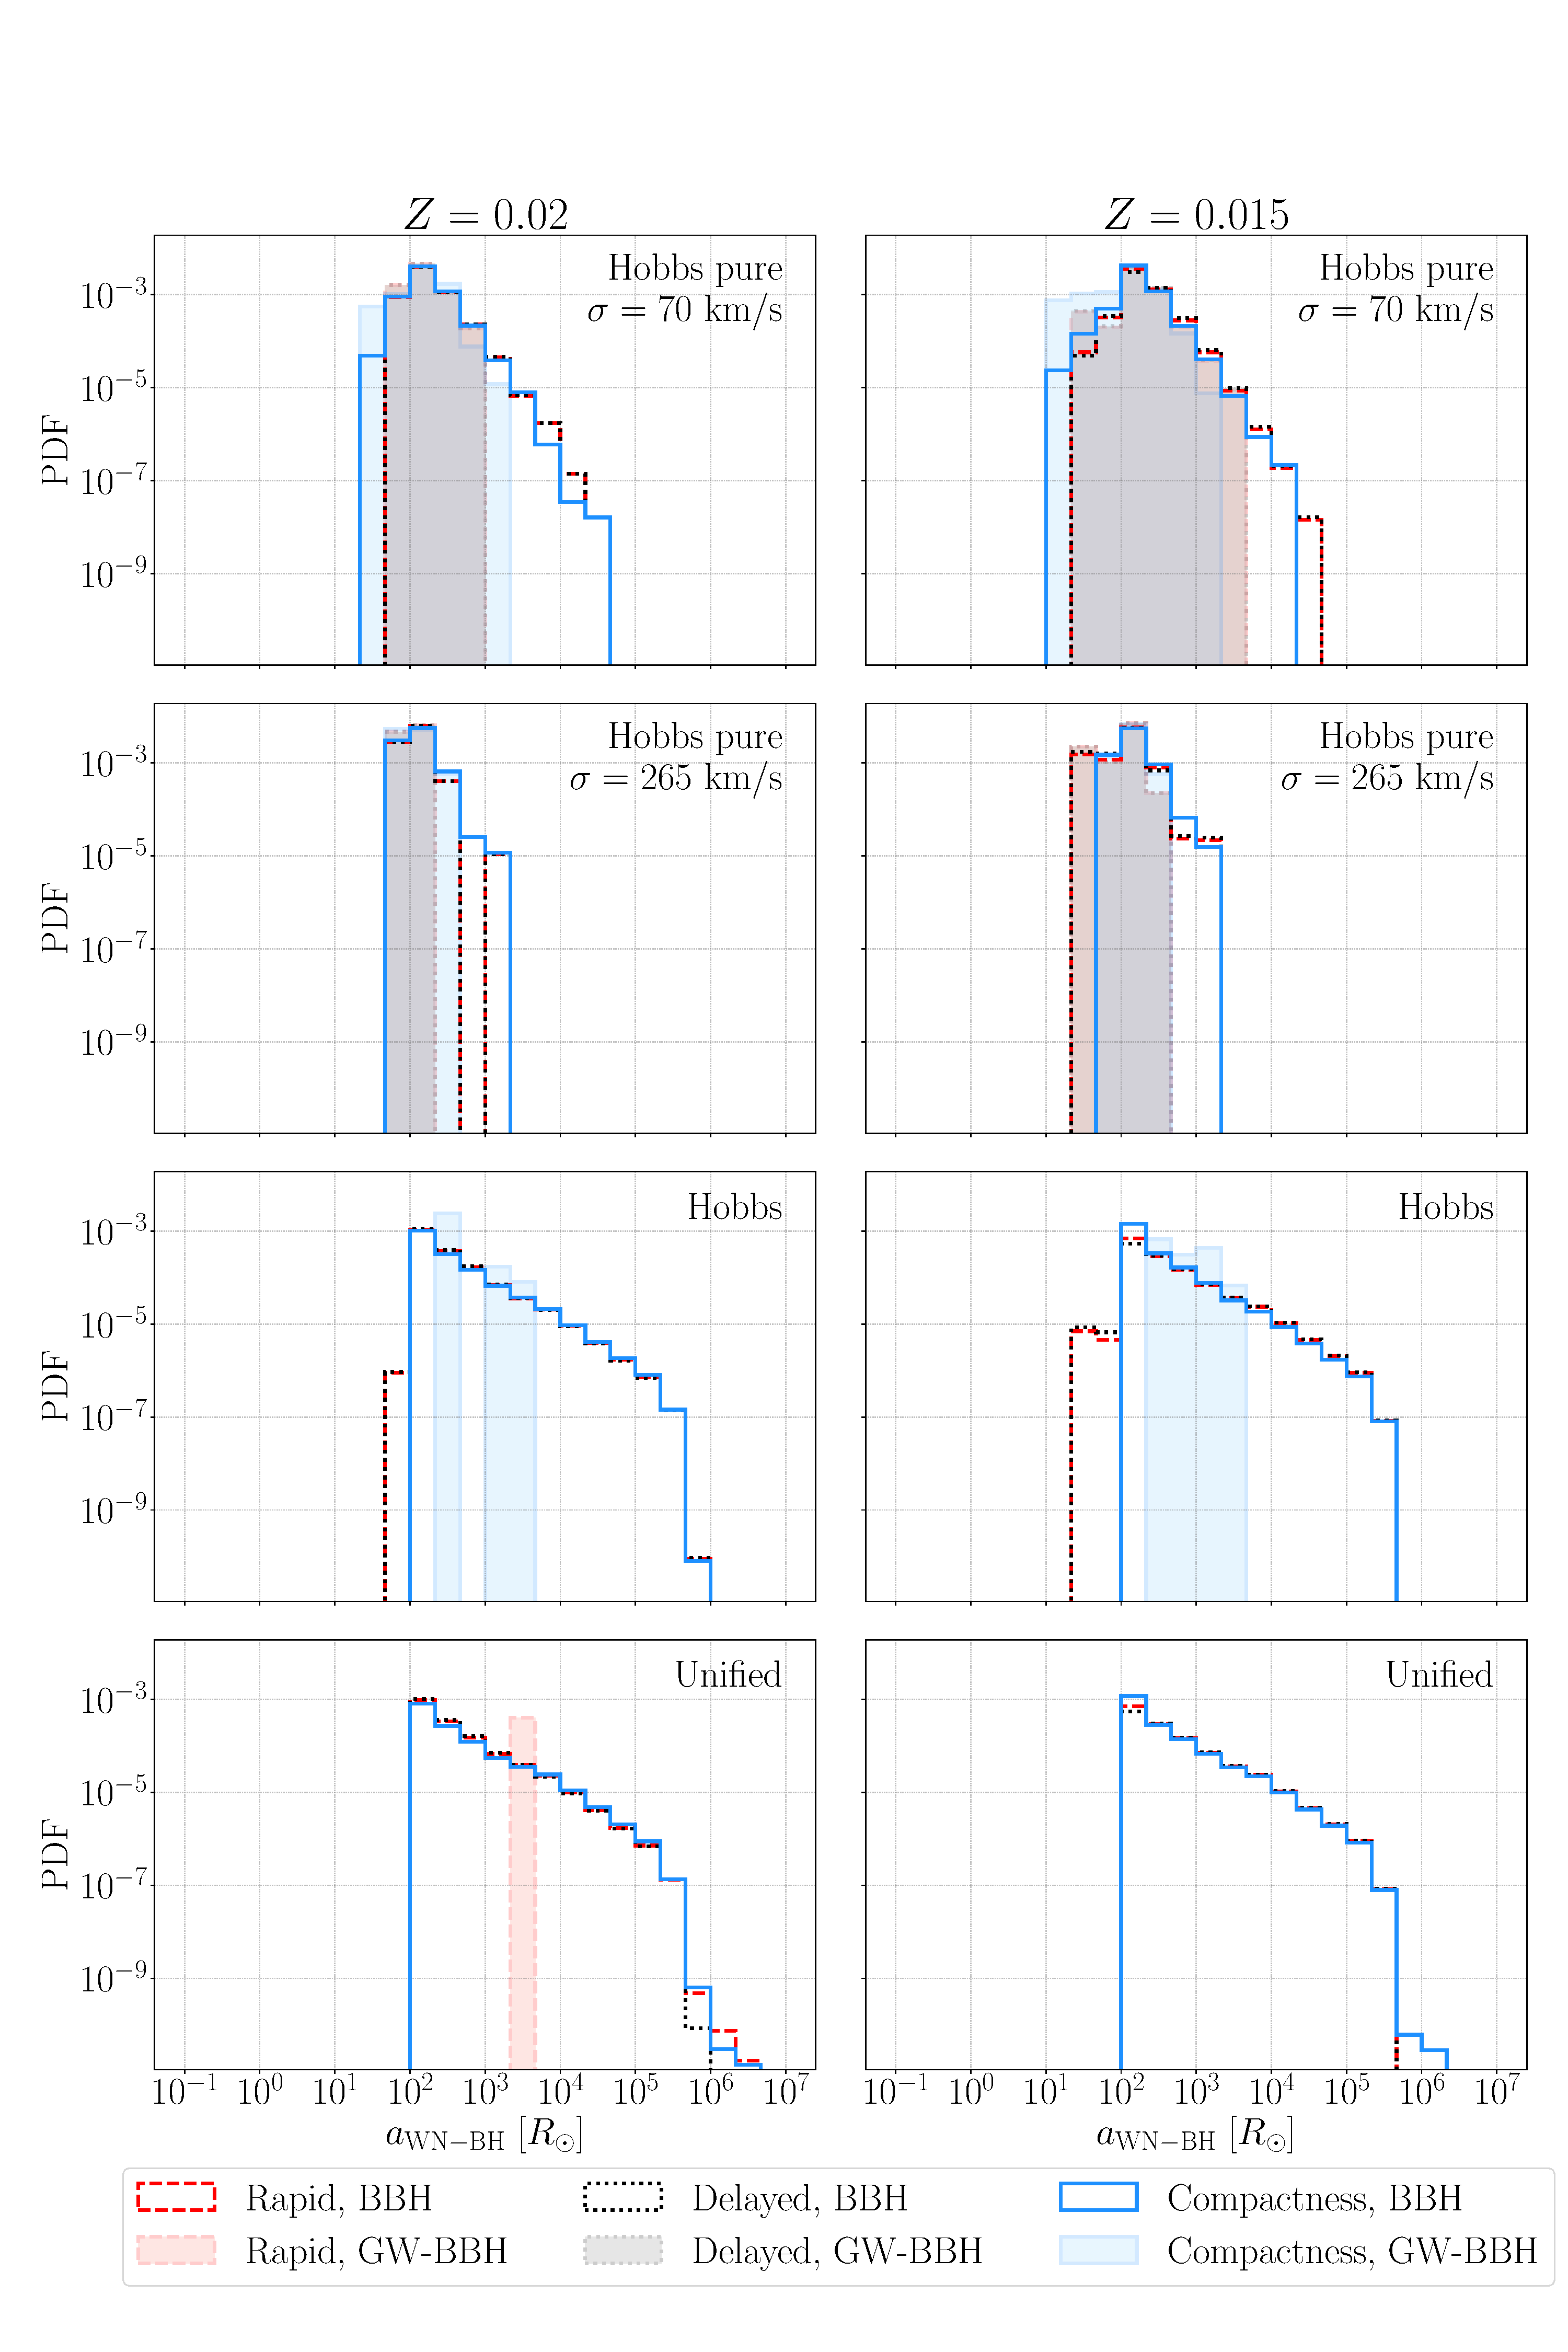
\includegraphics[width=\textwidth]{./images/WRBH-anonpureHe.pdf}	
	\caption{PDFs of semi-major axis $a$ at the beginning of the WN--BH phase for systems that will become BBHs or GW--BBHs after a WR--BH for different metallicities $Z$, CCSN models and supernova kick options (see Fig.\ \ref{fig:resultsM1prog} for line-styles and colours).}\label{fig:resultsWRBH-anonpureHe}
\end{figure}


\begin{figure}[h!]
	\centering
	\includegraphics[width=\textwidth]{./images/WRBH-RLfillWRnonpureHe.pdf}	
	\caption{PDFs of Wolf-Rayet Roche lobe filling $R/R_{\rm L}$ at the beginning of the WN--BH phase for systems that will become BBHs or GW--BBHs after a WR--BH for different metallicities $Z$, CCSN models and supernova kick options (see Fig.\ \ref{fig:resultsM1prog} for line-styles and colours). Bins are $R/R_{\rm L} = 1$ wide: most of WR--BH systems are not filling their Roche lobe. The stellar radius adopted is only a proxy for systems with active Roche lobe overflows (see Sec.\ \ref{subsec:masstransferSEVN}).}\label{fig:resultsWRBH-RLfillnonpureHe}
\end{figure}


\begin{figure}[h!]
	\centering
	\includegraphics[width=\textwidth]{./images/WRBH-MWRpureHe.pdf}	
	\caption{PDFs of masses of Wolf-Rayet WC- and WO-like stars $M_{\rm WCO}$ at the beginning of the WR--BH phase for systems that will become BBHs or GW--BBHs after a WR--BH for different metallicities $Z$, CCSN models and supernova kick options (see Fig.\ \ref{fig:resultsM1prog} for line-styles and colours).}\label{fig:resultsWRBH-MWRpureHe}
\end{figure}


\begin{figure}[h!]
	\centering
	\includegraphics[width=\textwidth]{./images/WRBH-apureHe.pdf}	
	\caption{PDFs of semi-major axis $a$ at the beginning of the WCO--BH phase for systems that will become BBHs or GW--BBHs after a WR--BH for different metallicities $Z$, CCSN models and supernova kick options (see Fig.\ \ref{fig:resultsM1prog} for line-styles and colours).}\label{fig:resultsWRBH-apureHe}
\end{figure}


\begin{figure}[h!]
	\centering
	\includegraphics[width=\textwidth]{./images/WRBH-RLfillpureHe.pdf}	
	\caption{PDFs of Wolf-Rayet Roche lobe filling $R/R_{\rm L}$ at the beginning of the WCO--BH phase for systems that will become BBHs (empty histograms) or GW--BBHs (filled histograms) at $Z=0.02$ (\emph{left}) or $Z=0.015$ (\emph{right}) for different CCSN models (\emph{rapid}, red dashed line; \emph{delayed}, black dotted line; \emph{compactness}, blue solid line) and supernova kicks (from top to bottom: \emph{hobbs pure} with $\sigma = 70$ km/s or $\sigma = 265$ km/s; \emph{hobbs} or \emph{unified} with $\sigma = 265$ km/s). The stellar radius adopted is only a proxy for systems with active Roche lobe overflows (see Sec.\ \ref{subsec:masstransferSEVN}).}\label{fig:resultsWRBH-RLfillpureHe}
\end{figure}

%%%% eccentricity %%%%%
\begin{figure}[h!]
	\centering
	\includegraphics[width=\textwidth]{./images/remeccentricity.pdf}	
	\caption{PDFs of final eccentricity $e_{\rm BBH}$ of BBHs or GW--BBHs after a WR--BH for different metallicities $Z$, CCSN models and supernova kick options (see Fig.\ \ref{fig:resultsM1prog} for line-styles and colours).}\label{fig:resultsRemEccentricity}
\end{figure}


%%%%%%% observability WR-BH %%%%
\begin{figure}[h!]
	\centering
	\includegraphics[width=\textwidth]{./images/WRBHtime.pdf}	
	\caption{PDFs for the time spent in the WR--BH configuration by systems that will become BBHs or GW--BBHs after a WR--BH for different metallicities $Z$, CCSN models and supernova kick options (see Fig.\ \ref{fig:resultsM1prog} for line-styles and colours).}\label{fig:resultsWRBH-time}
\end{figure}

\begin{figure}[h!]
	\centering
	\includegraphics[width=\textwidth]{./images/WRBH-P.pdf}	
	\caption{PDFs of period $P_{\rm WR-BH}$ at the beginning of the WR--BH phase for systems that will become BBHs or GW--BBHs after a WR--BH for different metallicities $Z$, CCSN models and supernova kick options (see Fig.\ \ref{fig:resultsM1prog} for line-styles and colours). Vertical black lines indicate 1 hour and 1 day thresholds.}\label{fig:resultsWRBH-P}
\end{figure}







\clearpage

These simulations could also explain the limited sample of observed WR--BH candidates. Recalling that we are already considering WR--BHs with the shortest periods allowed to avoid coalescence, the majority of them under-fill their Roche lobe (see the discussion in the previous paragraphs on Fig.\ \ref{fig:resultsWRBH-RLfillnonpureHe} and \ref{fig:resultsWRBH-RLfillpureHe}): even if, in principle, these systems could be observed because they have periods of hours or days, they are likely wind-fed systems with accretion inefficient to make them visible as X-ray binaries. Moreover, the systems considered here exist only for $\sim 2.5 - 15$ Myr before becoming BBHs (harder to detect), spending only $\sim 0.01 \sim 6\%$ of their life in the WR--BH configuration in the most optimistic case, in which they are GW--BBH progenitors.



\subsection{Compact remnants}\label{subsec:remnantsBBHsGWBBHs}
In this section, I will discuss the configuration of BBHs and GW--BBHs after the Wolf-Rayet star explodes and forms the secondary black hole. In particular, I will denote as primary $M_{\rm 1,BH}$ and secondary $M_{\rm 2,BH}$ black hole mass the ones formed from the star with the highest ($M_{\rm 1, ZAMS}$) and lowest ($M_{\rm 2, ZAMS}$) ZAMS mass, respectively.

\paragraph{Preference for equal mass systems $\boldsymbol{q_{\rm BBH} \sim 1}$}Similarly to other works in the literature \cite{giacobbomapelli2018_mobse_fryer}, Fig.\ \ref{fig:resultsqrem} highlights that BBHs formed in isolated environments are more likely to be equal-mass binaries. Nevertheless, many systems exhibit mass ratios $q_{\rm BBH}=M_{\rm 2, BH}/M_{\rm 1, BH} > 1$, further supporting the hypothesis that similar binaries underwent at least one mass transfer episode (other evidences were already presented and discussed in Sec.\ \ref{subsec:WRBHphaseBBHsGWBBHs}). In particular, GW--BBHs evolved with the \emph{compactness} model  more likely host  asymmetric mass systems because this CCSN option allows to form black holes lighter than the ones produced with the \emph{rapid} and \emph{delayed} models, as discussed in Sec.\ \ref{subsec:SNmodels}.

As a consequence, primary and secondary black hole masses shown in Fig.\ \ref{fig:resultsMBH1rem} and \ref{fig:resultsMBH2rem} lie in similar same mass ranges and do not exhibit relevant differences among BBHs and GW--BBHs, except for the presence of more massive systems at lower metallicities (where stellar winds are less effective, see Sec.\ \ref{subsec:stellarwinds}):  $M_{\rm 1, BH} \sim 3-25 (32)~\msun$ and $M_{\rm 2, BH} \sim 3-20 (28)~\msun$ for $Z=0.02 (0.015)$. These ranges do not change significantly depending on the assumed parameters, especially for primary black hole masses, even though the \emph{unified} kick model seems to favour the formation of lighter compact objects $\lesssim 20~\msun$. In general, the \emph{unified} and \emph{hobbs} models produce, on average, also lighter secondaries. 

As already discussed for the WN--BH fate in Sec.\ \ref{subsec:WRBHphaseBBHsGWBBHs}, these models produce kicks with magnitude often insufficient to significantly shrink the orbit of wide systems, thus favouring the formation of GW--BBHs only from binaries with orbits already tightened by mass transfer episodes. In particular, the closest orbits are the ones formed after common envelope episodes and the discussion on WCO--BH binaries suggested that these systems are indeed formed after a this process.



\paragraph{The role of eccentricity} The final semi-major axis distribution shown in Fig.\ \ref{fig:resultsarem} is almost identical to the one obtained at the beginning at the beginning of the WR--BH phase (considering Fig.\ \ref{fig:resultsWRBH-anonpureHe} and \ref{fig:resultsWRBH-apureHe} altogether). Therefore, the orbital separation is not strongly affected by the WR--BH evolution: WR--BH binaries do not undergo significant mass transfer episodes, even the few WN--BH that start in a Roche lobe overflow phase (see Fig.\ \ref{fig:resultsWRBH-RLfillnonpureHe}). Without a significant orbital change, WR--BH systems that are born in wide orbits $\sim 10^2 - 10^3~\rsun$ and evolved with damped supernova kicks (\emph{hobbs} and \emph{unified} models) can become GW--BBHs only if they become very eccentric $e_{\rm BBH} \sim 1$ after the second supernova event. 

As anticipated in Sec.\ \ref{subsec:WRBHphaseBBHsGWBBHs} for WN--BH systems, \texttt{SEVN} routines are more likely to produce high eccentric orbits for high-energy supernova kicks. The randomness introduced by these routines shifts towards $e_{\rm BBH} \sim 1$ the eccentricity PDFs for BBHs obtained with the \emph{hobbs pure} kicks, visible in Fig.\ \ref{fig:resultsRemEccentricity}. In contrast, binaries formed with damped kick options, as the \emph{hobbs} and \emph{unified} ones, do not significantly change their eccentricity with the supernova explosion. Given that most of WR--BHs evolve in circular orbits, the eccentricity PDFs for these kick options indeed favour the production of circular BBHs. However, the  PDFs of  GW--BBHs highlight the strong eccentricity dependence on the merging time ($t_{\rm GW} \propto (1-e^2)$, Eq. \ref{eq:tgw}) and show an additional and almost isolated peak at $e_{\rm BBH} \sim 1$. This bi-modality is present also in the GW--BBH eccentricity distribution for the less energetic \emph{hobbs pure} kicks, the ones obtained from a Maxwellian with a root-mean-square of $\sigma = 70$ km/s.

\clearpage



\begin{figure}[h]
	\centering
	\includegraphics[width=\textwidth]{./images/remM1.pdf}	
	\caption{PDFs of primary black hole masses $M_{\rm 1,BH}$ (formed from the initially more massive star $M_{\rm 1,ZAMS} \geq M_{\rm 2,ZAMS}$) for BBHs or GW--BBHs evolved through a WR--BH for different metallicities $Z$, CCSN models and supernova kick options (see Fig.\ \ref{fig:resultsM1prog} for line-styles and colours).}\label{fig:resultsMBH1rem}
\end{figure}

\begin{figure}[h]
	\centering
	\includegraphics[width=\textwidth]{./images/remM2.pdf}	
	\caption{PDFs of secondary black hole masses $M_{\rm 2, BH}$ (formed from the initially less massive star $M_{\rm 2, ZAMS} \leq M_{\rm 1, ZAMS}$) for BBHs or GW--BBHs evolved through a WR--BH for different metallicities $Z$, CCSN models and supernova kick options (see Fig.\ \ref{fig:resultsM1prog} for line-styles and colours).}\label{fig:resultsMBH2rem}
\end{figure}

\begin{figure}[h]
	\centering
	\includegraphics[width=\textwidth]{./images/remq.pdf}	
	\caption{PDFs of final mass ratio $q_{\rm BBH} = M_{\rm 2,BH}/M_{\rm 1,BH}$ for BBHs or GW--BBHs evolved through a WR--BH for different metallicities $Z$, CCSN models and supernova kick options (see Fig.\ \ref{fig:resultsM1prog} for line-styles and colours). Vertical black line marks systems with equal masses $q=1$.}\label{fig:resultsqrem}
\end{figure}

\begin{figure}[h]
	\centering
	\includegraphics[width=\textwidth]{./images/rema.pdf}	
	\caption{PDFs of final semi-major axis $a_{\rm BBH}$ of BBHs or GW--BBHs evolved through a WR--BH for different metallicities $Z$, CCSN models and supernova kick options (see Fig.\ \ref{fig:resultsM1prog} for line-styles and colours).}\label{fig:resultsarem}
\end{figure}



\clearpage




\section{Cyg X-3 as a GW--BBH progenitor at Z=0.015}\label{sec:CygX3vsGWBBHsproperties}

In Sec.\ \ref{sec:propertiesBBHsandGWBBHs}, I extensively discussed the statistical properties of BBHs and GW--BBHs, concluding that they are reasonably well-defined in the parameter space explored. In particular, CCSN and kick models influence the PDFs more than choosing $Z=0.02$ or $Z=0.015$: the only difference in the lower-metallicity systems is that they host heavier stars at later times, because of the less efficient winds. Therefore, I will focus hereafter on the evolution at $Z=0.015$, that is more representative of the true solar metallicity according to the measurements of Caffau et al.\ \cite{caffau2011solarmetallicity}.

In this section, I will focus on the properties of Cyg X-3 candidates that are GW--BBH progenitors: they represent more than $\gtrsim 75\%$ of all Cyg X-3 candidates; all of them for the majority of the parameter space explored (see Tab.\ \ref{tab:simulationresults}). I will discuss their role in the sub-populations of GW--BBHs binaries that emerge from the simulations. I will show the orbital properties of these systems at the ZAMS (Fig.\ \ref{fig:resultsCygX3progbinaries} and \ref{fig:resultsCygX3progM1M2GWBBHs}), at the beginning of the WR--BH phase (Fig.\ \ref{fig:resultsCygX3WRBHbinaries} and \ref{fig:resultsCygX3WRBHphaseGWBBHs}) and as BBH (Fig.\ \ref{fig:resultsCygX3rembinaries} and \ref{fig:resultsCygX3remBHBHGWBBHs}). Eventually, I will propose a synoptic comparison of the evolutionary stages for the fiducial kick model (Fig.\ \ref{fig:resultskickunified265Z015evolutionCygX3}) that will be adopted in the next section (Sec.\ \ref{fig:resultskickunified265Z015evolutionCygX3}). 




\subsection{Cyg X-3 progenitors}\label{subsec:ProgenitorsCygX3vsGWBBHs}
\paragraph{Similar initial masses} As shown in Fig.\ \ref{fig:resultsCygX3progbinaries} and \ref{fig:resultsCygX3progM1M2GWBBHs}, Cyg X-3 progenitors that will become GW--BBHs have ZAMS masses well-defined across the whole parameter space: $M_{\rm 1, ZAMS} \approx M_{\rm 2, ZAMS} \sim 30-40~\msun$. Even though the restricted mass range is a consequence of the boundaries adopted to classify a system as a Cyg X-3 candidate ($M_{\rm WR} = 8-14~\msun$ and $M_{\rm BH}=3-10~\msun$, see Sec.\ \ref{subsec:cygx3observations}), the ZAMS properties of Cyg X-3 fall in the most likely region to become a GW--BBH.

\paragraph{Short initial periods} In contrast, the initial orbital separation of Cyg X-3 systems that will become GW--BBHs is not always representative of the most likely initial condition for GW--BBH progenitors. However, both GW--BBH and Cyg X-3 binaries evolve from orbits with semi-major axis $a_{\rm ZAMS} \sim 10^1-10^3~\rsun$ and host massive stars $M_{\rm 1,ZAMS} + M_{\rm 2,ZAMS} \gtrsim 60~\msun$, thus, their initial period ranges from a few days to a few years (see Fig.\ \ref{fig:resultsCygX3progbinaries}).

\subsection{Cyg X-3 and GW--BBH sub-populations}\label{subsec:CygX3phasevsGWBBHs}
\paragraph{Cyg X-3 represents a physical sub-population} Fig.\ \ref{fig:resultsCygX3WRBHbinaries} and \ref{fig:resultsCygX3WRBHphaseGWBBHs} illustrate the beginning of the WR--BH phase for systems that will become BBHs and GW--BBHs, highlighting Cyg X-3 candidates that will form a GW--BBH. 

Cyg X-3 candidates cluster in Fig.\ \ref{fig:resultsCygX3WRBHbinaries} and \ref{fig:resultsCygX3WRBHphaseGWBBHs} because of the restrictive conditions imposed to classify them: $\mbh = 3-10~\msun$, $\mwr = 8-14~\msun$ and $P_{\rm WR-BH}=4.5-5.1$ hours (see Sec.\ \ref{subsec:cygx3observations}). Nevertheless, they show the same properties as a sub-population of GW--BBHs progenitors that is present in every combination of the parameter space. This sub-population also clusters at $P_{\rm WR-BH} \sim 5$ hours but allows to host more massive objects and includes total binary masses of $\sim 20-30~\msun$. Looking in more detail at Fig.\ \ref{fig:resultsCygX3WRBHphaseGWBBHs}, similar systems host a combination of black holes with masses $\mbh \sim 3-10~\msun$ and Wolf-Rayet stars with $\mwr \sim 10-20~\msun$. 

Fig.\ \ref{fig:resultsCygX3WRBHbinaries} indicates that this sub-population is separated from other two sub-populations. However, these latter clusters are present only for some combinations of the parameters space, suggesting that the sub-population of systems with properties similar to the Cyg X-3 candidates has indeed well-defined properties.

\paragraph{Other sub-populations of GW--BBHs} Systems evolved with the \emph{compactness} CCSN model are allowed to form black holes from lighter progenitors than the ones required for the \emph{rapid} and \emph{delayed} options (see Sec.\ \ref{subsec:SNmodels}). Therefore, only the \emph{compactness} model forms a second sub-population of binaries that have still short orbital periods (only few hours) but total binary mass of $\sim 10 - 15~\msun$. In fact, if the black hole masses are still in the $\mbh \sim 3-10~\msun$ range, the Wolf-Rayet stars have masses $\mwr \lesssim 10~\msun$, with few and rare exceptions (see the first two columns of Fig.\ \ref{fig:resultsCygX3WRBHphaseGWBBHs}). These stars will keep losing mass and eventually become so light to form a neutron star in place of a black hole according to the \emph{rapid} and \emph{delayed} CCSN models.\\

The last sub-population of GW--BBH progenitors has large orbital periods $\gtrsim 1$ day and wider orbits $a_{\rm WR-BH} \gtrsim 10~\rsun$. While binaries with properties similar to the other two sub-populations could \emph{only} become GW--BBH systems (if the Wolf-Rayet star formed a black hole and not a neutron star) because their orbit was already tight, this sub-population shares the same parameter space as BBHs: the larger orbit does not guarantee that if a BBH forms it will merge via gravitational wave emission within a Hubble time. 

The magnitude of the second supernova kick and the final eccentricity strongly determine whether similar systems will be able to become GW--BBHs or remain BBHs. As already discussed in Sec.\ \ref{sec:propertiesBBHsandGWBBHs}, the \emph{hobbs pure} option causes a larger variability in the kick magnitude and final orbital properties: it allows more systems with many different properties to become GW--BBHs and explains the wide scattering in the binary properties. Of course, the kicks should not be too much energetic in order not to disrupt the BBH, as shows the paucity of bound BBHs survived to the high magnitude of kicks generated with \emph{hobbs pure} option and $\sigma = 265$ km/s Maxwellian root-mean-square. 

In contrast, \emph{hobbs} and \emph{unified} kick models produce lower kicks and only few, if none, of the wide WR--BH binaries will become GW--BBHs. In this case, systems evolved with the \emph{rapid} and \emph{delayed} CCSN models have a higher probability to become GW--BBHs: starting from the same pre-SN mass, these CCSN options form lighter compact remnants with respect to the \emph{compactness} model and, according to the kick routines described in Sec.\ \ref{subsec:kicksSEVN}, lighter compact objects are more likely to receive strong kicks.




\subsection{Compact object binaries produced by Cyg X-3 progenitors}\label{subsec:RemnantsCygX3vsGWBBHs}
\paragraph{Slightly wider orbits} Wolf-Rayet stars at solar metallicities suffer strong stellar winds and decrease their mass, eventually exploding in a supernova event. The significant mass loss occurred from the beginning of the WR--BH phase ($\Delta M \lesssim 5~\msun$) causes wider orbits (see Sec.\ \ref{subsec:masstransfer}) and longer orbital periods. However, a comparison between the compact remnant orbital properties (Fig.\ \ref{fig:resultsCygX3rembinaries}) and the orbital properties at the beginning of the WR--BH phase (Fig.\ \ref{fig:resultsCygX3WRBHbinaries}) highlight almost negligible changes, with semi-major axis wider of only few solar radii and orbital periods few hours longer. 



\paragraph{A significant mass change} Aside from the eccentricity change already discussed in Sec.\ \ref{subsec:remnantsBBHsGWBBHs}, the major difference in the orbital properties of the resulting compact binary system is the lighter binary mass (see Fig.\ \ref{fig:resultsCygX3remBHBHGWBBHs}). The variation is strongly dependent on the CCSN model: if the black holes formed with the \emph{compactness} model retain $\sim 90\%$ of their pre-SN mass, the ones produced with the \emph{rapid} and \emph{delayed} models are $\lesssim 5-10~\msun$ lighter than their Wolf-Rayet progenitors at the beginning of the WR--BH configuration.

\paragraph{Sub-populations and Cyg X-3} The three sub-populations identified in the previous section Sec.\ \ref{subsec:CygX3phasevsGWBBHs} can still be identified but with a less clear separation. The most mixed populations are the ones generated with the \emph{hobbs pure} kick and \emph{rapid} or \emph{delayed} CCSN models: for these options the black hole mass and orbit strongly depend on minimal variations in the natal kick and CO mass (see Sec.\ \ref{subsec:SNmodels}). In contrast, damped kicks coupled with the \emph{compactness} CCSN model preserve at most the orbital properties of the pre-SN stage. Nevertheless, it seems that even for these kicks, the sub-populations are well-separated only in the WR--BH configuration, becoming more mixed in the compact remnant phase and indistinguishable in the ZAMS stage, as shown in the synoptic view of Fig.\ \ref{fig:resultskickunified265Z015evolutionCygX3}.

The BBH masses of Cyg X-3 candidate systems remain a representative low-mass limit of the sub-population identified in the previous section. However, the possible configurations and, in particular, the mass of the black holes produced by the Wolf-Rayet star $M_{\rm 2, BH}$, strongly depend on the CCSN model adopted: $M_{\rm 1, BH} \sim 5-7~\msun$ and $M_{\rm 2, BH}=5-10~\msun$ for the \emph{rapid}, $M_{\rm 1, BH} \sim 3-5~\msun$ and $M_{\rm 2, BH}=3-5~\msun$ for the \emph{delayed} and $M_{\rm 1, BH} \sim 5-8~\msun$ and $M_{\rm 2, BH}=8-13~\msun$ for the \emph{compactness}. Once again, the larger mass of the secondary black hole is a proxy for at least one mass transfer in the binary evolution, as is indeed the case for Cyg X-3 systems (see the discussion in the next section Sec.\ \ref{sec:resultsCygX3evo}).


\clearpage
%%%%%%%%% progenitors %%%%%%
\begin{figure}[h!]
	\centering
	\includegraphics[width=\textwidth]{./images/kickcompare_prog_015.pdf}	
	\caption{Orbital properties at ZAMS of BBHs (grey-scaled histogram) and GW--BBHs (coloured histogram) evolved through a WR--BH configuration compared with the progenitors of Cyg X-3 that will become GW--BBHs (cyan dots). The panels explore the parameter space at $Z=0.015$ for different supernova kicks (from top to bottom: \emph{hobbs pure} with $\sigma = 70$ km/s; \emph{hobbs pure}, \emph{hobbs} or \emph{unified} with $\sigma = 265$ km/s) and CCSN models (from left to right: \emph{rapid}, \emph{delayed} or \emph{compactness}). Black diagonal lines indicate orbital periods of 1 year, 1 day or 1 hour.}\label{fig:resultsCygX3progbinaries}
\end{figure}

\begin{figure}[h!]
	\centering
	\includegraphics[width=\textwidth]{./images/kickcompare_progM1M2_015.pdf}	
	\caption{ZAMS masses of primary $M_{\rm 1, ZAMS}$ and secondary $M_{\rm 2, ZAMS}$ progenitors of GW--BBHs (histogram) evolved through a WR--BH configuration compared with the progenitors of Cyg X-3 that will become GW--BBHs (cyan dots). The panels explore the parameter space at $Z=0.015$ for different supernova kicks (from top to bottom: \emph{hobbs pure} with $\sigma = 70$ km/s; \emph{hobbs pure}, \emph{hobbs} or \emph{unified} with $\sigma = 265$ km/s) and CCSN models (from left to right: \emph{rapid}, \emph{delayed} or \emph{compactness}). Black diagonal line indicates equal mass systems $q_{\rm ZAMS}=M_{\rm 2, ZAMS}/M_{\rm 1,ZAMS} = 1$.}\label{fig:resultsCygX3progM1M2GWBBHs}
\end{figure}



%%%%%%%% WR--BH %%%%%%%%%%5
\begin{figure}[h!]
	\centering
	\includegraphics[width=\textwidth]{./images/kickcompare_WRBH_015.pdf}	
	\caption{Orbital properties at the beginning of the WR--BH phase for BBHs and GW--BBHs progenitors compared with the ones for Cyg X-3 candidates that will become GW--BBHs. The panels explore the parameter space at $Z=0.015$ for different supernova kicks and CCSN models, as in Fig.\ \ref{fig:resultsCygX3progbinaries}. Black diagonal lines indicate orbital periods of 1 year, 1 day or 1 hour.}\label{fig:resultsCygX3WRBHbinaries}
\end{figure}

\begin{figure}[h!]
	\centering
	\includegraphics[width=\textwidth]{./images/kickcompare_MWRMBH_015.pdf}	
	\caption{Mass of Wolf-Rayet stars $M_{\rm WR}$ and black holes $M_{\rm BH}$ at the start of the WR--BH phase for all GW--BBHs progenitors and only for GW--BBH progenitors evolved as Cyg X-3 candidates. The panels explore the parameter space at $Z=0.015$ for different supernova kicks and CCSN models, as in Fig.\ \ref{fig:resultsCygX3progM1M2GWBBHs}. Black diagonal line indicates equal mass systems $q=\mwr/\mbh = 1$. The bin width is $1~\msun$ for $M_{\rm BH}$ and $2~\msun$ for $M_{\rm WR}$. }\label{fig:resultsCygX3WRBHphaseGWBBHs}
\end{figure}




%%%%%%%%%% remnants %%%%%%%%%%%
\begin{figure}[h!]
	\centering
	\includegraphics[width=\textwidth]{./images/kickcompare_rem_015.pdf}	
	\caption{Orbital properties after the second supernova of GW--BBHs evolved through a WR--BH configuration compared with the ones of Cyg X-3 candidates that become GW--BBHs. The panels explore the parameter space at $Z=0.015$ for different supernova kicks and CCSN models, as in Fig.\ \ref{fig:resultsCygX3progbinaries}. Black diagonal lines indicate orbital periods of 1 year, 1 day or 1 hour.}\label{fig:resultsCygX3rembinaries}
\end{figure}

\begin{figure}[h!]
	\centering
	\includegraphics[width=\textwidth]{./images/kickcompare_MBHMBH_015.pdf}	
	\caption{Masses of primary $M_{\rm 1, BH}$ and secondary $M_{\rm 2, BH}$ black holes of GW--BBHs evolved through a WR--BH configuration compared with compact remnants of Cyg X-3 that became GW--BBHs. The panels explore the parameter space at $Z=0.015$ for different supernova kicks and CCSN models, as in Fig.\ \ref{fig:resultsCygX3progM1M2GWBBHs}. Black diagonal line indicates equal mass systems $q_{\rm BBH}=M_{\rm 2,BH}/M_{\rm 1,BH} = 1$.}\label{fig:resultsCygX3remBHBHGWBBHs}
\end{figure}



%%%%%%%%%% fiducial kick %%%%%%%%%%%%%%
\begin{figure}[h!]
	\centering
	\includegraphics[width=\textwidth]{./images/binary_unified265_015.pdf}
	\caption{ZAMS (\emph{top}), beginning of WR--BH phase (\emph{middle}) and compact remnant configurations (\emph{bottom}) for Cyg X-3 fiducial model: \emph{unified} kick and solar metallicity $Z=0.015$. Orbital properties of BBHs (grey-scaled histogram) and GW--BBHs (coloured histogram) undergoing a WR--BH evolution are compared to the ones of Cyg X-3 candidates that will become GW--BBHs (cyan dots) for the three CCSN models explored (from left to right: \emph{rapid}, \emph{delayed} or \emph{compactness}).}\label{fig:resultskickunified265Z015evolutionCygX3}
\end{figure}





\clearpage

\section{Cyg X-3 evolution}\label{sec:resultsCygX3evo}
In this section I will explain in detail the evolutionary processes and orbital properties that allow Cyg X-3 candidates to become GW--BBHs. I will focus on the formation channels for the fiducial model ($Z=0.015$, \emph{unified} kick model and \emph{compactness} CCSN option), discussing its validity. I will compare these evolutionary channels with the ones for the \emph{rapid} and \emph{delayed} CCSN models, illustrated in Appendix~\ref{appsec:CYgX3GWBBHs}.

\subsection{The fiducial model}\label{subsec:fiducialCygX3}
\paragraph{Metallicity} In Sec.\ \ref{sec:propertiesBBHsandGWBBHs} I showed that choosing $Z=0.02$ or $Z=0.015$ does not significantly change the PDFs for BBHs and GW--BBHs: the only difference is in the stellar wind efficiency and causes up to a $\Delta M \lesssim 5~\msun$ shift in the stellar and black hole masses. Therefore, in Sec.\ \ref{sec:CygX3vsGWBBHsproperties} I chose $Z=0.015$ as the representative solar metallicity (as also suggested by Caffau et al.\ \cite{caffau2011solarmetallicity}) and studied the impact of CCSN and kick models.

\paragraph{Kick} The discussion carried out in Sec.\ \ref{sec:CygX3vsGWBBHsproperties} showed that kicks generated with the \emph{hobbs pure} option are often too much energetic to represent the evolution of binaries hosting black holes. In contrast, the down-scaling of the kick magnitude adopted in the \emph{hobbs} and \emph{unified} models are more physically motivated and do not strongly modify the orbital properties, as expected. Even if systems evolved with the \emph{unified} and \emph{hobbs} models exhibit similar properties and both models account for the mass that falls back onto the compact object, I will choose as fiducial the \emph{unified} kick option because it re-scales the kick magnitude also with the compact object mass, thus, follows a more accurate description of the linear angular momentum conservation (see Sec.\ \ref{subsec:kicksSEVN}).

\paragraph{CCSN} The \emph{rapid} and \emph{delayed} CCSN models determine the compact object mass by means of piece-wise functions that strongly depend on the CO mass of the progenitor star (see Sec.\ \ref{subsec:SNmodels}). As shown in Fig.\ \ref{fig:remnants} and discussed in Sec.\ \ref{sec:propertiesBBHsandGWBBHs} and Sec.\ \ref{sec:CygX3vsGWBBHsproperties}, black holes formed in this work often have progenitors with pre-SN mass $M_{\rm pre-SN} \sim 7-20~\msun$, thus falling in the range where the \emph{rapid} and \emph{delayed} models differ the most from the \emph{compactness} model. In particular, similar progenitors evolved with the first two CCSN options form black holes up to $\sim 15~\msun$ lighter than the ones formed with the \emph{compactness} model. Moreover, the \emph{rapid} and \emph{delayed} models have higher chances to form neutron stars rather than black holes from pre-SN masses in the aforementioned mass range. Therefore, even though the \emph{compactness} model favours the formation of heavier compact objects (see Fig.\ \ref{fig:resultskickunified265Z015evolutionCygX3}) and, in particular, of black holes, I will choose it as the fiducial CCSN model.





\subsection{A mass-transfer driven evolution}\label{subsec:CygX3masstransferdrivenevo}
\paragraph{Initial masses} The discussion carried out in Sec.\ \ref{subsec:ProgenitorsCygX3vsGWBBHs} and referred to Fig.\ \ref{fig:resultsCygX3progM1M2GWBBHs} indicated that Cyg X-3 progenitors have similar initial masses of $M_{\rm ZAMS} \sim 30-40~\msun$ across the whole parameter space explored. The 22 Cyg X-3 candidates of the fiducial model considered here and shown in Fig.\ \ref{fig:resultsCygX3masstransferM1M2} are no exception to this and formed with primary stars $M_{\rm 1, ZAMS}$ only $\lesssim 5~\msun$ more massive than the secondaries $M_{\rm 2, ZAMS}$ (empty circles).

\paragraph{A necessary first mass transfer} All Cyg X-3 candidates of the fiducial model enter a Roche lobe overflow episode while the secondary star is still in the main sequence phase. However, the stability of the RLO is strongly affected by the possible combinations of the initial semi-major axis, primary mass and, most importantly, mass ratio.\\

Binaries born in tight orbits with semi-major axis $a_{\rm ZAMS} \lesssim 10^2\,{}\rsun$ are the ones where the primary fills sooner its Roche lobe and enters the RLO routine only after $\sim 4 - 4.5$ Myr from the ZAMS configuration. Donor stars are still in the main sequence phase and, having masses similar to their companions, the RLO begins as a stable one ($q \leq q_{\rm crit}$, see Sec.\ \ref{subsec:masstransferSEVN}). Fig.\ \ref{fig:resultsCygX3masstransferM1M2}, \ref{fig:resultsCygX3masstransferSemimajor} and \ref{fig:resultsCygX3masstransferRLfill} show that nine Cyg X-3 candidates have these orbital properties: seven of them undergo a \emph{stable} RLO (blue dashed lines) while the other two will, at some point, transform the stable RLO into a common envelope evolution (red dashed lines while in the stable RLO phase and dotted red lines in the CE).

The systems that terminate the stable RLOs are the ones born with the most asymmetric mass ratios $q_{\rm ZAMS}=M_{\rm 2, ZAMS}/M_{\rm 1,ZAMS} \sim 0.85-0.9$, lighter secondaries and primary stars that rapidly evolve from the start of the H-shell burning (\texttt{BSE} phase = 2, see Tab.\ \ref{tab:phasesqcritSEVN}) to the beginning of the core-He burning (\texttt{BSE} phase = 4), avoiding the interpolation through the late phase of the H-shell burning (\texttt{BSE} phase = 3). 

In contrast, systems that start with more similar and heavier masses $q_{\rm ZAMS} \sim 0.9-0.93$ have more efficient stellar winds: at the beginning of the RLO, the primary is lighter than the ones previously described, with a mass lower than $M_{\rm 1,ZAMS} \lesssim 35~\msun$. Less massive stars evolve more slowly (see Sec.\ \ref{subsec:stellarevo}) and with different properties, causing these primaries to be interpolated by \texttt{SEVN} through the last part of the H-shell burning (\texttt{BSE} phase = 3) and, thus, entering an unstable RLO. In fact, according to Tab.\ \ref{tab:phasesqcritSEVN}, the criterion $q \geq q_{\rm crit}$ to enter an unstable RLO only depends on the \texttt{BSE} phase and, only for late H-shell burning stars, $q_{\rm crit}$ is lowered to account for the formation of a significant He core.

A similar finding further confirms what was extensively discussed in Sec.\ \ref{subsec:masstransfer}: the current mass transfer routines implemented in population-synthesis codes need to be revised. However, regardless of the problems in current mass transfer models, the simulations clearly highlight that a first mass transfer event is fundamental to produce a Cyg X-3 candidate that can become a GW--BBH: the primary main sequence star needs to fill its Roche lobe and transfer mass to the secondary in a stable or unstable process, eventually resulting in a Wolf-Rayet star (light-grey filled squares).\\

Systems in wider initial orbits $a_{\rm ZAMS} \sim 100 - 3000~\rsun$ can also become Cyg X-3 progenitors but, evolving in wider orbits, they can enter the RLO phase only when the primary has already expanded its radius after the core-He burning stage: all these primaries overfill their Roche lobe while in the Hertzsprung-gap phase. Similarly to the tightest systems, the binaries with more asymmetric mass ratios and lighter secondaries ($M_{\rm 2, ZAMS} \sim 26-28~\msun$) rapidly evolve through the core-He burning phase, skipping the late H-shell burning and terminating a stable RLO. In contrast, heavier and more symmetric systems have primaries that are interpolated through the giant branch phase and enter a common envelope.\\

Overall, the CE evolution does not modify the secondary, well-constrained with a mass of $M_{\rm 2} \sim 30-35~\msun$, but removes the hydrogen envelope of the primary and produces a Wolf-Rayet star with mass $M_{\rm 1, WR} \sim 14-15~\msun$, equal to the He-core mass of the progenitor, which was initially of $M_{\rm 1, ZAMS} \sim 33~\msun$. While the unstable RLO is short-lived and lasts only $0.005-0.2$ Myrs, stable mass transfer occurs on a longer timescale of $\sim 1$ Myr (with the exception of the stable mass transfer initiated by Hertzsprung-gap stars, which become core-He burning Wolf-Rayet stars in $\lesssim 0.5$ Myrs). 

Moreover, stable RLOs allow the secondary to accrete $\sim 7-10~\msun$ but produce stars lying in different mass ranges. If the primary overfills its Roche lobe as a main sequence star with $M_1 \gtrsim 35~\msun$ it will produce a Wolf-Rayet with $M_{1, WR} \sim 12-14~\msun$ and the secondary $M_2 \gtrsim 30~\msun$ will become a main sequence star of $M_{2} \sim 37-45~\msun$. In contrast, primaries entering the stable RLO as Hertzsprung-gap stars are already lighter $M_1 \sim 28-32~\msun$ and will produce Wolf-Rayet stars of only $M_{\rm 1, WR} \sim 9-12~\msun$, with main sequence companions of only $M_2 \sim 32-36~\msun$. Overall, at the end of the first mass transfer, binaries undergoing stable RLOs retain more mass with respect to the systems produced through common envelope evolution, but host lighter Wolf-Rayet stars. 


\paragraph{The secondary mass} Fig.\ \ref{fig:resultsCygX3masstransferM1M2} highlights that \emph{all} Cyg X-3 candidates enter the WR - BH configuration as a result of a CE evolution. At least for GW--BBHs belonging to the same sub-population of Cyg X-3 (see Sec.\ \ref{sec:CygX3vsGWBBHsproperties}), this evolution confirms the hints discussed in Sec.\ \ref{subsec:WRBHphaseBBHsGWBBHs}: the Wolf-Rayet star in the WR--BH configuration (dark-grey circle) is the result of a common envelope evolution, at the end of which the primary star explodes forming the black hole (black-filled star). In particular, only systems that start a CE with a black hole progenitor mass of $\sim 8-10~\msun$ and secondary mass of $\sim 26-35~\msun$ have the right properties to become WR--BH systems that could be classified as Cyg X-3 candidates ($\mbh = 3-10~\msun$ and $\mwr = 8-14~\msun$, see Sec.\ \ref{subsec:cygx3observations}).

Primary stars evolved though a first common envelope or through a stable RLO from a Hertzsprung-gap donor already form with these properties: after $\sim 0.5$ Myr they undergo a common envelope and reach the Cyg X-3 configuration. In contrast, binaries that entered a completely stable RLO with main sequence primaries produced secondaries that are too massive. Therefore, only these binaries require a third mass transfer process (a stable RLO from the secondary) to become Cyg X-3 progenitors. As shown in Fig.\ \ref{fig:resultsCygX3masstransferRLfill} these systems exit the first stable RLO as wind-fed binaries with a secondary star that is already filling its Roche lobe more than 50\%: in $\lesssim 0.2$ Myr it overfills its Roche lobe remaining a main sequence star and loses up to $\lesssim 15~\msun$. Since the accretor is a Wolf-Rayet star, its strong stellar winds are assumed to efficiently eject the mass incoming from the donor, thus, no mass is accreted and the orbit widens (even though it remains close to $\sim 100~\rsun$).




\begin{figure}[h!]
	\centering
	\includegraphics[width=.9\textwidth]{./images/com_Mass_1_Mass_0_BHBH_GW_WRBH_cyg_x-3--Ko17.pdf}
	\caption{Mass of the primary star as a function of the secondary star for the Cyg X-3 candidates evolved with the fiducial model: $Z=0.015$, \emph{unified} supernova kick and \emph{compactness} CCSN. Starting from the ZAMS (empty circles), the primaries enter a stable mass transfer (dashed thick lines) that either remains stable (blue line) or becomes unstable (red line) and results in a common envelope (dotted red line). The primaries become Wolf-Rayet stars (light-grey squares) and the secondaries enter a second RLO (solid thick lines), again stable (blue) or unstable (red). After a necessary common envelope, the secondaries become Wolf-Rayet stars (dark-grey dots) and the primaries form a black hole (black stars). At the end of the WR--BH phase, also the secondary forms a black hole (yellow star) and a BBH is born (small black dots). Thin lines mark the phases without active mass transfer and are coloured according to the initial semi-major axis, visible in Fig.\ \ref{fig:resultsCygX3masstransferSemimajor}.}\label{fig:resultsCygX3masstransferM1M2}
\end{figure}

\begin{figure}[t!]
	\centering
	\includegraphics[width=\textwidth]{./images/BWorldtime_Semimajor_BHBH_GW_WRBH_cyg_x-3--Ko17.pdf}
	\caption{Semi-major axis as a function of the time from the ZAMS for Cyg X-3 candidates evolved with the fiducial model: $Z=0.015$, \emph{unified} supernova kick and \emph{compactness} CCSN. Thick lines highlight active mass transfer phases, as described in Fig.\ \ref{fig:resultsCygX3masstransferM1M2}.}\label{fig:resultsCygX3masstransferSemimajor}
\end{figure}

\begin{figure}[b!]
		\centering
		\includegraphics[width=.7\textwidth]{./images/RLfill1_RLfill0_BHBH_GW_WRBH_cyg_x-3--Ko17.pdf}	
    \caption{Roche lobe filling fraction of primary star $R_1/R_{\rm L,1}$ as a function of the Roche lobe filling fraction of the secondary star $R_2/R_{\rm L,2}$ for Cyg X-3 candidates evolved with the fiducial model: $Z=0.015$, \emph{unified} supernova kick and \emph{compactness} CCSN. Thick lines highlight active mass transfer phases, as described in Fig.\ \ref{fig:resultsCygX3masstransferM1M2}. The plot shows from the ZAMS to the formation of the WR--BH binary and is only illustrative of the mass transfer events: I recall that for $R \geq R_{\rm L}$, the stellar radius is used only for stellar wind computations and is no more representative of the star size, limited by \texttt{SEVN} to the Roche lobe radius (see Sec.\ \ref{subsec:masstransferSEVN}).}\label{fig:resultsCygX3masstransferRLfill}
\end{figure}




\paragraph{Mass transfer and Cyg X-3 sub-families} Even though most of the primaries start with $M_{\rm 1,ZAMS} \sim 35-40~\msun$, the ones undergoing only common envelope evolution lose less mass than the ones that went through two stable RLOs: the first produce primary black holes with $M_{\rm 1, BH} \sim 6.3-7.5~\msun$ while the latter $M_{\rm 2, BH} \sim 5-6.2~\msun$. Similar differences in the formation channels and final properties are visible also in the systems evolved with \emph{rapid} and \emph{delayed} CCSN models in Fig.\ \ref{fig:resultsCygX3masstransferM1M2rapid} and \ref{fig:resultsCygX3masstransferM1M2delayed}. In particular, the \emph{delayed} model forms neutron stars instead of black holes for the systems undergoing stable RLOs and, therefore, identifies as Cyg X-3 candidates only the systems undergoing two common envelopes. Similar results are obtained also varying metallicity and supernova kick models, even though the higher metallicity binaries $Z=0.02$ show a more uniform spread in the compact object masses (see Sec.\ \ref{sec:CygX3vsGWBBHsproperties}).

Even though systems undergoing two common envelopes, or two RLOs and one common envelope seem to form two sub-families with distinguishable evolutionary pathways, it is possible that it is only a consequence of the current approximate mass transfer models. For instance, the three systems that entered the first stable RLO as Hertzsprung-gap donors could either form a third sub-family or highlight that a rigid classification in the evolutionary scenario is not meaningful with current models. In fact,they evolve through only one stable RLO and one common envelope, starting from lighter ZAMS masses and populating both black hole families.




\subsection{Observable properties}\label{subsec:CygX3}
\paragraph{A portion of the WR--BH phase} Fig.\ \ref{fig:resultsCygX3masstransferPeriod} shows that Cyg X-3 candidates are observable as Cyg X-3 $\lesssim 0.2$ Myr after the formation of the WR--BH configuration. They last in the Cyg X-3 configuration for a variable amount of time $\sim 0.01-0.1$ Myr  (black thick lines), depending on whether they satisfy the Cyg X-3 conditions starting from the lower or upper bound in the period range adopted $P_{\rm WR-BH}=4.5-5.1$ hours. In fact, these candidates start the WR--BH phase with a period of $P_{\rm i, WR-BH} \sim 2.5-4.7$ hours and then increase it as the Wolf-Rayet stellar winds disperse mass. Binaries born in tight orbits $a_{\rm ZAMS} \lesssim 100~\rsun$ maintain shorter periods and end the WR--BH configuration with $P_{\rm f,WR-BH} \sim 5-6$ hours after 0.4 Myrs. In contrast, wider systems $a_{\rm ZAMS} \sim 100 - 3000~\rsun$ evolve for additional 0.1 Myrs and reach final periods of $P_{\rm f,WR-BH} \sim 7-8.5$ hours.

\paragraph{Wind-fed systems} Fig.\ \ref{fig:resultsCygX3masstransferwindfedduration} illustrates the Roche lobe filling fraction of the Wolf-Rayet star member of the WR--BH phase as it loses mass due to its strong stellar winds. As reported in the previous section Sec.\ \ref{subsec:CygX3masstransferdrivenevo}, WR--BH systems considered here are all formed after a common envelope. Fig.\ \ref{fig:resultsCygX3masstransferSemimajor} shows that the orbit at the end of the CE phase has semi-major axis of only $a \sim 2-4~\rsun$, comparable to the Wolf-Rayet radius. Therefore, WR--BH systems start as powerful wind-fed systems with a Wolf-Rayet filling its Roche lobe $\sim 80\%$. As the WR star evolves, it loses mass, reduces its size and widens the orbit, eventually decreasing the Roche lobe filling fraction. When the systems become visible as Cyg X-3 ($\mwr = 8-14~\msun$), the Wolf-Rayet is still powering the black hole accretion disk through wind mass losses, even if less efficiently because it is now filling only $\sim 60-80\%$ of its Roche lobe. 







\newpage
\begin{figure}[t!]
	\centering
	\includegraphics[width=\textwidth]{./images/BWorldtime_Period_BHBH_GW_WRBH_cyg_x-3--Ko17.pdf}
	\caption{Period evolution in the WR--BH phase for Cyg X-3 candidates evolved with the fiducial model: $Z=0.015$, \emph{unified} supernova kick and \emph{compactness} CCSN. Thick black lines highlight the visibility as Cyg X-3 system while thin lines are coloured according to the initial semi-major axis of Fig.\ \ref{fig:resultsCygX3masstransferSemimajor}.}\label{fig:resultsCygX3masstransferPeriod}
\end{figure}

\begin{figure}[b!]
		\centering
		\includegraphics[width=\textwidth]{./images/WR_Mass_1_RLfill1_BHBH_GW_WRBH_cyg_x-3--Ko17.pdf}	
    \caption{Roche lobe filling fraction of the Wolf-Rayet in the WR--BH phase as a function of its mass for Cyg X-3 candidates evolved with the fiducial model: $Z=0.015$, \emph{unified} supernova kick and \emph{compactness} CCSN. Thick black lines highlight the visibility as Cyg X-3 system while thin lines are coloured according to the initial semi-major axis of Fig.\ \ref{fig:resultsCygX3masstransferSemimajor}.}\label{fig:resultsCygX3masstransferwindfedduration}
\end{figure}










\chapter{Conclusions}
In this thesis, I simulated 24 sets of physically motivated binary populations, each containing $10^6$ systems, by means of the population-synthesis code \texttt{SEVN} (see Sec.\ \ref{sec:initialconditionsSEVN}). Each set was characterized by a different combination of the 24-dimension parameter space explored and  included two possible values for the solar metallicity ($Z=0.02$ and $Z=0.015$), three core-collapse supernova models (\emph{rapid}, \emph{delayed} and \emph{compactness}) and four supernova kick options (\emph{hobbs pure} with Maxwellian root-mean-square of $\sigma=70$ km/s; \emph{hobbs pure}, \emph{hobbs} and \emph{unified} with $\sigma=265$ km/s), described in Sec.\ \ref{sec:SEVN}. The primary aim of this work was to study how this parameter space influences the role of Wolf-Rayet--black hole binaries (WR--BHs) as progenitors of the binary black holes (BBHs) that have been observed with the LIGO and Virgo gravitational wave detectors (see Sec.\ \ref{ch:GW}). The secondary aim was to characterize the evolution of the only WR--BH candidate observed as X-ray binary in the Milky Way, Cyg X-3, and understand if it could be a proxy for BBH mergers (see Sec.\ \ref{ch:WR--BH}). \\

I found that at solar metallicity $\gtrsim 90 \%$ of the BBHs merging within a Hubble time via gravitational wave emission have evolved through a WR--BH configuration. A similar fate is common also to $\gtrsim 75 \%$ of the Cyg X-3 candidates found in my simulations (see Tab.\ \ref{tab:simulationresults}). Moreover, Cyg X-3 systems became a reliable proxy to trace the evolution of at least one sub-population of BBH mergers: those with final total binary mass of $\sim 10-30~\msun$, semi-major axis $\lesssim 10~\rsun$, and orbital period ranging from a few hours to a few days (see Sec.\ \ref{sec:CygX3vsGWBBHsproperties}). These results are robust and independent on the combination of metallicity, core-collapse or supernova kick model assumed. \\

Binaries similar to Cyg X-3 reach the WR--BH configuration after one common envelope evolution and one or two previous additional stable mass transfer events. Usually, the aforementioned processes are either a common envelope or a stable Roche lobe overflow (RLO) started by the star initially more massive, with the possibility that the first stable RLO leaves a companion star still too much massive and forces it to start a second stable RLO to reduce its mass before the final common envelope. 

The occurrence and type of mass transfer events prior to the last common envelope depend on the parameters assumed, but are more sensible to the core-collapse supernova model. In fact, some of the assumed core-collapse supernova models favour the formation of neutron stars in place of black holes and cause some of the Cyg X-3 systems to become neutron star - black hole binaries, with properties similar to the ones found by Belczynski et al.\ \cite{Belczynski2013_CygX-3fate}. However, the current models implemented in population-synthesis codes to determine the stability of RLO events have proven to be inadequate and need to be revised, as already highlighted by many authors in the literature including Gallegos-Garcia et al.\  \cite{gallegos2021MESAvspopsynth}.\\

This work highlights that, at solar metallicity, WR--BH binaries are a necessary configuration to produce BBH mergers, characterizing their last evolutionary stage prior to the second black hole formation. Most of the short period period WR--BH binaries ($P \lesssim 10$ hours) are visible as wind-fed X-ray binaries. Binaries with wider orbits, hosting mostly H-rich Wolf-Rayet stars, could be detected also in the RLO configuration. Nevertheless, systems with $a \gtrsim 10~\rsun$ not only are unlikely to undergo significant mass transfer and be visible as X-ray binaries, but could also become BBH mergers only if they received supernova kicks energetic enough to produce highly eccentric orbits  (see Sec.\ \ref{subsec:CygX3phasevsGWBBHs}).\\


Overall, the results that I obtained in this thesis underline that further and more accurate observations of WR--BH binaries at solar metallicity are expected to provide useful insights in the characterization of the progenitors of BBH mergers. In particular, accurate measurements of the spins of  Wolf-Rayet stars could improve the mass transfer models and possibly solve the tension highlighted by Fishbach \& Kalogera between the spin distribution of X-ray binaries and BBHs observed by the LIGO-Virgo Collaboration \cite{HMXBH_spins2021}.











%%%%%%%%%%%%%%%%%%%%%%%%%%%%%%%%%%%%%%%%%%%%%%%%%
%%%%%%%%% Appendix %%%%%%%%%%%%%%%%%%%%%%%%%%%%%%
%%%%%%%%%%%%%%%%%%%%%%%%%%%%%%%%%%%%%%%%%%%%%%%%
\begin{appendices}
%\noappendicestocpagenum
%\addappheadtotoc

%\chapter{Figures}\label{app:figures}
%\section{Properties of BBHs and GW--BBHs}\label{subapp:BBHandGWBBHproperties}
%\subsection{Progenitors}\label{subapp:progenitorsGWBBH}
%Fig.\ \ref{fig:resultsM1prog}, \ref{fig:resultsM2prog}, \ref{fig:resultsqprog} and \ref{fig:resultsaprog} characterize the initial ZAMS configuration for BBHs and GW--BBHs progenitors undergoing a WR--BH evolution, as discussed in Sec.\ \ref{subsec:progenitorsBBHsGWBBHs}.








%\subsection{WR--BH phase}\label{subapp:WRBHphaseGWBBH}
%Figures %\ \ref{fig:resultsWRBH-MBH}, \ref{fig:resultsWRBH-MWRnonpureHe}, \ref{fig:resultsWRBH-MWRpureHe}, \ref{fig:resultsWRBH-anonpureHe}, \ref{fig:resultsWRBH-apureHe}, \ref{fig:resultsWRBH-RLfillnonpureHe}, \ref{fig:resultsWRBH-RLfillpureHe}, 
%\ref{fig:resultsWRBH-time} and \ref{fig:resultsWRBH-P} characterize the beginning of the WR--BH configuration for progenitors of BBHs and GW--BBHs, as discussed in Sec.\ \ref{subsec:WRBHphaseBBHsGWBBHs}.









%\subsection{Compact remnants}\label{subapp:remnantsGWBBH}
%Fig.\ \ref{fig:resultsMBH1rem}, \ref{fig:resultsMBH2rem}, \ref{fig:resultsqrem}, \ref{fig:resultsarem} characterize the configuration of BBHs and GW--BBHs after the Wolf-Rayet in WR--BH systems explodes and forms the secondary black hole, as discussed in Sec.\ \ref{subsec:remnantsBBHsGWBBHs}.








%%%%%%%%%%%%%%%%%%%%%%%%%%%%%%%%%%%%%%%%
%\section{Cyg X-3 as a GW--BBH progenitor at Z=0.015}\label{appsec:CYgX3GWBBHs}
%\subsection{Cyg X-3 progenitors}\label{appsubsec:ProgenitorsCygX3vsGWBBHs}
%Fig.\ \ref{fig:resultsCygX3progbinaries} and \ref{fig:resultsCygX3progM1M2GWBBHs} characterize the ZAMS configuration of Cyg X-3 progenitors that will become GW--BBHs, as discussed in Sec.\ \ref{subsec:ProgenitorsCygX3vsGWBBHs}.

%\subsection{Cyg X-3 compact remnants}\label{appsubsec:RemnantsCygX3vsGWBBHs}
%Fig.\ \ref{fig:resultsCygX3rembinaries} and \ref{fig:resultsCygX3remBHBHGWBBHs} characterize the final configuration of Cyg X-3 candidate systems that became GW--BBHs, as discussed in Sec.\ \ref{subsec:RemnantsCygX3vsGWBBHs}.



\chapter{Alternative models for Cyg X-3 evolution}\label{appsec:CYgX3GWBBHs}
%\subsection{Mass transfer for different CCSN models}
Fig.\ \ref{fig:resultsCygX3masstransferM1M2rapid} and \ref{fig:resultsCygX3masstransferM1M2delayed} illustrate the evolutionary pathways of Cyg X-3 candidates that form a GW--BBH according to the \emph{rapid} or \emph{delayed} CCSN model, respectively. These systems are evolved assuming the fiducial metallicity $Z=0.015$ and supernova kick \emph{unified} and serve as a comparison with the fiducial \emph{compactness} model shown in Fig.\ \ref{fig:resultsCygX3masstransferM1M2}.

\begin{figure}
	\centering
	\includegraphics[width=.9\textwidth]{./images/rap_Mass_1_Mass_0_BHBH_GW_WRBH_cyg_x-3--Ko17.pdf}
	\caption{Mass of the primary star as a function of the secondary for the Cyg X-3 candidates evolved with the fiducial metallicity ($Z=0.015$) and kick model (\emph{unified}) but adpoting the \emph{rapid} CCSN. Starting from the ZAMS (empty circles), the primaries enter a stable mass transfer (dashed thick lines) that either remains stable (blue line) or becomes unstable (red line) and results in a common envelope (dotted red line). The primaries become Wolf-Rayet stars (light-grey squares) and the secondaries enter a second RLO (solid thick lines), again stable (blue) or unstable (red). After a necessary common envelope, the secondaries become Wolf-Rayet stars (dark-grey dots) and the primaries form a black hole (black stars). At the end of the WR--BH phase, also the secondary forms a black hole (yellow star) and a BBH is born (small black dots). Thin lines mark the phases without active mass transfer and are coloured according to the initial semi-major axis, with a colour coding similar to Fig.\ \ref{fig:resultsCygX3masstransferSemimajor}.}\label{fig:resultsCygX3masstransferM1M2rapid}
\end{figure}

\begin{figure}
	\centering
	\includegraphics[width=.9\textwidth]{./images/del_Mass_1_Mass_0_BHBH_GW_WRBH_cyg_x-3--Ko17.pdf}
	\caption{Mass of the primary star as a function of the secondary for the Cyg X-3 candidates evolved with the fiducial metallicity ($Z=0.015$) and kick model (\emph{unified}) but adpoting the \emph{delayed} CCSN. Starting from the ZAMS (empty circles), the primaries enter an unstable Roche lobe overflow (red thick dashed lines) that results in a common envelope (red dotted line). The primaries become Wolf-Rayet stars (light-grey squares) and the secondaries enter a second unstable Roche lobe overflow (red thick solid lines) ending in a common envelope. The secondaries become Wolf-Rayet stars (dark-grey dots) and the primaries form a black hole (black stars). At the end of the WR--BH phase, also the secondary forms a black hole (yellow star) and a BBH is born (small black dots). Thin lines mark the phases without active mass transfer and are coloured according to the initial semi-major axis, with a colour coding similar to Fig.\ \ref{fig:resultsCygX3masstransferSemimajor}.}\label{fig:resultsCygX3masstransferM1M2delayed}
\end{figure}








\chapter{Acronyms}
\begin{tabular}{ll}
BBH & Binary black hole \\
BH & Black hole \\
CCSN & Core-collapse supernova \\
CDF & Cumulative density function \\
CE & Common envelope \\
GW  & Gravitational wave \\
GW--BBH & Binary black hole that will merge via GW emission within a Hubble time \\
HG & Hertzsprung - gap star\\
HMXB & High-mass X-ray binary \\
HR diagram & Hertzsprung-Russell diagram\\
LBV & luminous blue variable \\
LMXB & Low-mass X-ray binary \\
LTE & Local thermodynamic equilibrium \\
LVC & LIGO-Virgo collaboration \\
ISCO & Innermost circular orbit \\
MRD & Merger rate density \\
PDF & Probability density function \\
RLO & Roche lobe overflow \\
SN & Supernova \\
WC, WCO,  WO & Sub-types of Wolf-Rayet stars without hydrogen spectral lines \\
WN, WNE, WNL & Sub-types of Wolf-Rayet stars with hydrogen spectral lines \\
WR & Wolf-Rayet star \\
WR--BH & Binary composed of a Wolf-Rayet and a black hole \\
ZAMS & Zero age main sequence star \\

\end{tabular}
\end{appendices}



\printbibliography[heading=bibintoc]
\end{document}
















































